% !TeX root = ./thesis.tex
% !TEX encoding = UTF-8 Unicode
% !TEX program = latexmk
\documentclass{dissertation}


\definecolor{medium-gray}{HTML}{666666}
\definecolor{Burgundy}{RGB}{144, 0, 32}


%%% Public TikZ libraries
\pdfmapfile{=ua1.map} % hack for pdf insertion
% Provides math enviroments, math symbols and more things useful for math.
\usepackage{amsmath,mathtools,empheq}
\usepackage{amsthm}
\usepackage{thmtools}
\usepackage{thm-restate}
\usepackage{ bm, nicefrac}
\usepackage{thmtools}
\usepackage{bigints}
\usepackage{longtable}
\usepackage{pdflscape}
\usepackage[printonlyused, smaller]{acronym}
\usepackage{venndiagram} % draw Venn
\usepackage{neuralnetwork} % dreaw ANNs
\usepackage{qtree} % draw trees
\usepackage{tikz}
\usepackage[makeroom]{cancel}% cancel terms in equations
\usetikzlibrary{calc}
% https://tex.stackexchange.com/a/114770
\usepackage{etoolbox}
\robustify\setcounter
\robustify\addtocounter
\robustify\setlength
\robustify\addtolength

\usepackage{epsdice} % draw dices
% \usepackage{enumerate}

\usepackage[brazilian, english, british]{babel} % Sets the language used. Essential for proper hyphenation. Translates key words like 'figure' or 'table'. Note that 'english' is American English.

\usepackage{soul} %to add strike through functionality
\usepackage{listings}
\usepackage{pdfpages} % allows the inclusion of pdf pages as part of the document
 % need to create subfigures with captions

% % latexsym, amscd,
% \usepackage{graphicx} % Provides inclusion of graphics and a proper interface for '\in­clude­graph­ics'.
% % Su­per­sedes 'epsfig' and 'graphics'.

% \usepackage[shortlabels]{enumitem} % Provides control over list environments. Supersedes 'enumerate', which gives enumerate environment an optional argument which determines the style in which the counter is printed.

% \usepackage[all]{hypcap} % Anchors links to the beginning of their respective floats. Load after hyperref.

% % \usepackage{pgfplots}  make simpler the inclusion of plots in your documents.
% % \pgfplotsset{compat=1.8}
% % \pgfplotscreateplotcyclelist{smart}{%
% %   tangoplum,semithick,every mark/.append style={fill=tangoplum!80!black},mark=*\\%
% %   tangogreen,semithick,every mark/.append style={fill=tangogreen!80!black},mark=square*\\%
% %   tangoorange,semithick,every mark/.append style={fill=tangoorange!80!black},mark=otimes*\\%
% %   tangoblue,semithick,mark=star\\%
% %   tangobutter,semithick,every mark/.append style={fill=tangobutter!80!black},mark=diamond*\\%
% %   tangored,semithick,every mark/.append style={solid,fill=tangored!80!black},mark=*\\%
% % }
% % \pgfplotsset{cycle list name=smart}





% % -------

% \usepackage{wrapfig} % wraps figures in text


% % \usepackage{amsmath}
% \usepackage{amssymb} % to have symbols like \therefore
% % \usepackage[strict]{changepage} % adjust margins for images
% \usepackage{tikz} % used by venndiagram package
% \usetikzlibrary{patterns, matrix,chains,positioning,decorations.pathreplacing,arrows}
% \usepackage{calc} % needed for largeimage

% \captionsetup{format=plain, font=small, labelfont=bf}
% \usepackage{makeidx}\makeindex

% \usepackage[export]{adjustbox}
% % \usepackage[mathscr]{euscript}
% % \let\euscr\mathscr\let\mathscr\relax % just so we can load this and rsfs
% % \usepackage[scr]{rsfso}
% % \usepackage{svg}
% % \usepackage{tocloft}




% % \usepackage[shortlabels]{enumitem} % shortlabels provide compatibility with enumerate package - enumitem permits change margin of item
% % % \setlist[enumerate,1]{label={\bfseries\arabic*.}} % alow sublist referencing
% % \setlist[enumerate,2]{label={\bfseries\alph*)},ref={\bfseries\theenumi\alph*)}}
% % \usepackage{amsthm} % add theorem definition


%%%%% NEW MATH DEFINITIONS %%%%%

\usepackage{bm}
\usepackage{bigints}
\usepackage{nicefrac}
\usepackage{venndiagram}



% Mark sections of captions for referring to divisions of figures
\newcommand{\figleft}{{\em (Left)}}
\newcommand{\figcenter}{{\em (Center)}}
\newcommand{\figright}{{\em (Right)}}
\newcommand{\figtop}{{\em (Top)}}
\newcommand{\figbottom}{{\em (Bottom)}}
\newcommand{\captiona}{{\em (a)}}
\newcommand{\captionb}{{\em (b)}}
\newcommand{\captionc}{{\em (c)}}
\newcommand{\captiond}{{\em (d)}}

% Highlight a newly defined term
\newcommand{\newterm}[1]{{\bf #1}}
% \newcommand{\eqdef}{{\overset{\text{def}}{=}}}
\newcommand{\eqdef}{{\triangleq}}

% \let\oldint\int
% \renewcommand{\int}{{\bigintssss}}
\renewcommand{\leq}{{~\leqslant ~}}
\renewcommand{\geq}{{~\geqslant ~}}

% Figure reference, lower-case.
\def\figref#1{figure~\ref{#1}}
% Figure reference, capital. For start of sentence
\def\Figref#1{Figure~\ref{#1}}
\def\twofigref#1#2{figures \ref{#1} and \ref{#2}}
\def\quadfigref#1#2#3#4{figures \ref{#1}, \ref{#2}, \ref{#3} and \ref{#4}}
% Section reference, lower-case.
\def\secref#1{section~\ref{#1}}
% Section reference, capital.
\def\Secref#1{Section~\ref{#1}}
% Reference to two sections.
\def\twosecrefs#1#2{sections \ref{#1} and \ref{#2}}
% Reference to three sections.
\def\secrefs#1#2#3{sections \ref{#1}, \ref{#2} and \ref{#3}}
% Reference to an equation, lower-case.
\def\eqref#1{eq.~\ref{#1}}
% Reference to an equation, upper case
\def\Eqref#1{Equation~\ref{#1}}
% A raw reference to an equation---avoid using if possible
\def\plaineqref#1{\ref{#1}}
% Reference to a chapter, lower-case.
\def\chapref#1{chapter~\ref{#1}}
% Reference to an equation, upper case.
\def\Chapref#1{Chapter~\ref{#1}}
% Reference to a range of chapters
\def\rangechapref#1#2{chapters\ref{#1}--\ref{#2}}
% Reference to an algorithm, lower-case.
\def\algref#1{algorithm~\ref{#1}}
% Reference to an algorithm, upper case.
\def\Algref#1{Algorithm~\ref{#1}}
\def\twoalgref#1#2{algorithms \ref{#1} and \ref{#2}}
\def\Twoalgref#1#2{Algorithms \ref{#1} and \ref{#2}}
% Reference to a part, lower case
\def\partref#1{part~\ref{#1}}
% Reference to a part, upper case
\def\Partref#1{Part~\ref{#1}}
\def\twopartref#1#2{parts \ref{#1} and \ref{#2}}

\def\ceil#1{\lceil #1 \rceil}
\def\floor#1{\lfloor #1 \rfloor}
\def\truth{{\mathbb{1}}}
\newcommand{\train}{\mathcal{D}}
\newcommand{\valid}{\mathcal{D_{\mathrm{valid}}}}
\newcommand{\test}{\mathcal{D_{\mathrm{test}}}}

\def\eps{{\epsilon}}

% Matrix
\def\mSigma{{\bm{\Sigma}}}
\def\mA{{\bm{A}}}
\def\mB{{\bm{B}}}
\def\mC{{\bm{C}}}
\def\mD{{\bm{D}}}
\def\mE{{\bm{E}}}
\def\mF{{\bm{F}}}
\def\mG{{\bm{G}}}
\def\mH{{\bm{H}}}
\def\mI{{\bm{I}}}
\def\mJ{{\bm{J}}}
\def\mK{{\bm{K}}}
\def\mL{{\bm{L}}}
\def\mM{{\bm{M}}}
\def\mN{{\bm{N}}}
\def\mO{{\bm{O}}}
\def\mP{{\bm{P}}}
\def\mQ{{\bm{Q}}}
\def\mR{{\bm{R}}}
\def\mS{{\bm{S}}}
\def\mT{{\bm{T}}}
\def\mU{{\bm{U}}}
\def\mV{{\bm{V}}}
\def\mW{{\bm{W}}}
\def\mX{{\bm{X}}}
\def\mY{{\bm{Y}}}
\def\mZ{{\bm{Z}}}


% Vectors
\def\vmu{{\bm{\mu}}}
\def\vtheta{{\bm{\theta}}}
\def\va{{\bm{a}}}
\def\vb{{\bm{b}}}
\def\vc{{\bm{c}}}
\def\vd{{\bm{d}}}
\def\ve{{\bm{e}}}
\def\vf{{\bm{f}}}
\def\vg{{\bm{g}}}
\def\vh{{\bm{h}}}
\def\vi{{\bm{i}}}
\def\vj{{\bm{j}}}
\def\vk{{\bm{k}}}
\def\vl{{\bm{l}}}
\def\vm{{\bm{m}}}
\def\vn{{\bm{n}}}
\def\vo{{\bm{o}}}
\def\vp{{\bm{p}}}
\def\vq{{\bm{q}}}
\def\vr{{\bm{r}}}
\def\vs{{\bm{s}}}
\def\vt{{\bm{t}}}
\def\vu{{\bm{u}}}
\def\vv{{\bm{v}}}
\def\vw{{\bm{w}}}
\def\vx{{\bm{x}}}
\def\vy{{\bm{y}}}
\def\vz{{\bm{z}}}

% Outcomes
\def\rmu{{\mu}}
\def\rtheta{{\theta}}
\def\ra{{a}}
\def\rb{{b}}
\def\rc{{c}}
\def\rd{{d}}
\def\re{{e}}
\def\rf{{f}}
\def\rg{{g}}
\def\rh{{h}}
\def\ri{{i}}
\def\rj{{j}}
\def\rk{{k}}
\def\rl{{l}}
\def\rm{{m}}
\def\rn{{n}}
\def\ro{{o}}
\def\rp{{p}}
\def\rq{{q}}
\def\rr{{r}}
\def\rs{{s}}
\def\rt{{t}}
\def\ru{{u}}
\def\rv{{v}}
\def\rw{{w}}
\def\rx{{x}}
\def\ry{{y}}
\def\rz{{z}}
% Sets
\def\sOmega{{\mathbb{\Omega}}}
\def\sPhi{{\mathbb{\Phi}}}
\def\sA{{\mathbb{A}}}
\def\sB{{\mathbb{B}}}
\def\sC{{\mathbb{C}}}
\def\sD{{\mathbb{D}}}
% Don't use a set called E, because this would be the same as our symbol
% for expectation.
\def\sF{{\mathbb{F}}}
\def\sG{{\mathbb{G}}}
\def\sH{{\mathbb{H}}}
\def\sI{{\mathbb{I}}}
\def\sJ{{\mathbb{J}}}
\def\sK{{\mathbb{K}}}
\def\sL{{\mathbb{L}}}
\def\sM{{\mathbb{M}}}
\def\sN{{\mathbb{N}}}
\def\sO{{\mathbb{O}}}
\def\sP{{\mathbb{P}}}
\def\sQ{{\mathbb{Q}}}
\def\sR{{\mathbb{R}}}
\def\sS{{\mathbb{S}}}
\def\sT{{\mathbb{T}}}
\def\sU{{\mathbb{U}}}
\def\sV{{\mathbb{V}}}
\def\sW{{\mathbb{W}}}
\def\sX{{\mathbb{X}}}
\def\sY{{\mathbb{Y}}}
\def\sZ{{\mathbb{Z}}}

% Random variables
\def\rvA{{\mathit{A}}}
\def\rvB{{\mathit{B}}}
\def\rvC{{\mathit{C}}}
\def\rvD{{\mathit{D}}}
\def\rvE{{\mathit{E}}}
\def\rvF{{\mathit{F}}}
\def\rvG{{\mathit{G}}}
\def\rvH{{\mathit{H}}}
\def\rvI{{\mathit{I}}}
\def\rvJ{{\mathit{J}}}
\def\rvK{{\mathit{K}}}
\def\rvL{{\mathit{L}}}
\def\rvM{{\mathit{M}}}
\def\rvN{{\mathit{\eta}}}
\def\rvO{{\mathit{O}}}
\def\rvP{{\mathit{P}}}
\def\rvQ{{\mathit{Q}}}
\def\rvR{{\mathit{R}}}
\def\rvS{{\mathit{S}}}
\def\rvT{{\mathit{T}}}
\def\rvU{{\mathit{U}}}
\def\rvV{{\mathit{V}}}
\def\rvW{{\mathit{W}}}
\def\rvX{{\mathit{X}}}
\def\rvY{{\mathit{Y}}}
\def\rvZ{{\mathit{Z}}}


% The true underlying data generating distribution
\newcommand{\pdata}{p_{\textrm{data}}}
% The empirical distribution defined by the training set
\newcommand{\ptrain}{\hat{p}_{\textrm{data}}}
\newcommand{\Ptrain}{\hat{P}_{\textrm{data}}}
% The model distribution
\newcommand{\pmodel}{p_{\textrm{model}}}
\newcommand{\Pmodel}{P_{\textrm{model}}}
\newcommand{\ptildemodel}{\tilde{p}_{\texrm{model}}}
% Stochastic autoencoder distributions
\newcommand{\pencode}{p_{\textrm{encoder}}}
\newcommand{\pdecode}{p_{\textrm{decoder}}}
\newcommand{\precons}{p_{\textrm{reconstruct}}}

\newcommand{\KL}{D_{\mathrm{KL}}}
\newcommand{\Var}{\mathrm{Var}}
\newcommand{\Cov}{\mathrm{Cov}}
\DeclareMathOperator*{\argmax}{arg\,max}
\DeclareMathOperator*{\argmin}{arg\,min}
\DeclareMathOperator{\Tr}{Tr}
\let\ab\allowbreak

\newcommand{\lang}{\mathrm{L}}
\newcommand{\E}{\mathbb{E}}
\newcommand{\LH}{\mathcal{L}}
\newcommand{\Real}{\sR}
\newcommand{\Natural}{\sN}
\renewcommand{\AA}{\mathcal{A}}
\renewcommand{\SS}{S}
\newcommand{\DD}{D}
\newcommand{\CC}{\sC}
\newcommand{\XX}{\mathcal{X}}
\newcommand{\aXX}{\sA_{\rvX}}
\newcommand{\aZZ}{\sA_{\rvZ}}
\newcommand{\aYY}{\sA_{\rvY}}
\newcommand{\YY}{\mathcal{Y}}
% \newcommand{\YY}{\sA_{\rvY}}
\newcommand{\HH}{\mathcal{H}}
\newcommand{\LL}{\mathcal{L}}
\newcommand{\OO}{\mathcal{O}}
\newcommand{\NN}{\mathcal{N}}
\newcommand{\UU}{\mathcal{U}}
\newcommand{\PXY}{P(\rvX,\rvY)}
\newcommand{\pxy}{p(x,y)}
\newcommand{\Ix}{I_{\rvX}}
\newcommand{\Iy}{I_{\rvY}}
\newcommand{\IXZ}{I[{\rvZ};{\rvX}]}
\newcommand{\IZX}{I[{\rvZ};{\rvX}]}
\newcommand{\IYZ}{I[{\rvZ};{\rvY}]}
\newcommand{\IZY}{I[{\rvZ};{\rvY}]}
\newcommand{\IXY}{I[{\rvX};{\rvY}]}
\newcommand{\IYX}{I[{\rvX};{\rvY}]}
\newcommand{\IZN}{I[{\rvZ};{\rvN}]}
\newcommand{\INZ}{I[{\rvZ};{\rvN}]}
\newcommand{\IWD}{I[{\rvW};{\rvD}]}
\newcommand{\IDW}{I[{\rvW};{\rvD}]}

\newcommand{\HX}{H[{\rvX}}
\newcommand{\HY}{H[{\rvY}}
\newcommand{\HYX}{H[{\rvY}|{\rvX}]}
\newcommand{\HYZ}{H[{\rvY}|{\rvZ}]}

% Information Theory
\newcommand{\src}{\rvS}
\newcommand{\srcsymb}{\rs} % a source  outcome
% \renewcommand{\alph}[1]{\sA_{#1}}
\newcommand{\srcalph}{\sA_{\rvS}}
\newcommand{\srcrate}{R_{\rvS}}
\newcommand{\srcblk}{\src^{n}}
\newcommand{\enc}{\rvX}
\newcommand{\encrate}{\sR_{\rvX}}
\newcommand{\encvec}{\vx}
\newcommand{\encsymb}{\rx}
\newcommand{\encblk}{\enc^{k}}
\newcommand{\encalph}{\sA_{\rvX}}
\newcommand{\dec}{\rvY}
\newcommand{\decsymb}{\ry}
\newcommand{\decalph}{\sA_{\rvY}}
\newcommand{\decvec}{\vy}
\newcommand{\typicalset}{\sT_{\epsilon}^{(n)}}
\newcommand{\jointlyset}{\sJ_{\epsilon}^{(n)}}
\newcommand{\noise}{\rvN}

\newcommand{\circled}[1]{\tikz[baseline=(char.base)]{
            \node[shape=circle,draw,inner sep=2pt] (char) {#1};}}

% https://tex.stackexchange.com/a/114770
\robustify\setcounter
\robustify\addtocounter
\robustify\setlength
\robustify\addtolength

\definecolor{RoyalBlue}{cmyk}{1,0.5,0,0}
\definecolor{Black}{cmyk}{0,0,0,0}
\definecolor{alertred}{rgb}{0.80,0.12,0.12}
\definecolor{linkgreen}{RGB}{0,166,0}


\graphicspath{{./Images/}{./figures/}{./tikzpictures/}}

\newrobustcmd*{\fullfullcite}{%
    \AtNextCite{%
        \AtEachCitekey{%
            \defcounter{maxnames}{99}%
            \DeclareNameAlias{labelname}{given-family}%
        }%
    }%
    \fullcite
}


% \renewcommand{\cite}[1]{\sidecite{#1}}

% to fix problem with toc
% \AtBeginDocument{\addtocontents{toc}{%
%   \protect\vspace{\dimexpr\cftbeforepartskip-\cftbeforechapskip\relax}%
% }}

% \setlength{\cftbeforechapskip}{10pt}
% \renewcommand{\cftchapafterpnum}{\vspace{6pt}}
% \newcommand{\bt}[1]{\textbf{#1}}


% \renewcommand{\sectionmark}[1]{\markright{\textsc{\thesection}\enspace\spacedlowsmallcaps{#1}}}

% \newlength\largefigure
% % to create a new length
% % \setlength{\largefigure}{\columnwidth+\marginparsep+\marginparwidth}
% \setlength{\largefigure}{\textwidth+\marginparsep+\marginparwidth}

% \def\changemargin#1#2{\list{}{\rightmargin#2\leftmargin#1}\item[]}
% \let\endchangemargin=\endlist



\DeclareMathOperator*{\SumInt}{%
\mathchoice%
  {\ooalign{$\displaystyle\sum$\cr\hidewidth$\displaystyle\bigintsss$\hidewidth\cr}}
  {\ooalign{\raisebox{.14\height}{\scalebox{.7}{$\textstyle\sum$}}\cr\hidewidth$\textstyle\bigintsss$\hidewidth\cr}}
  {\ooalign{\raisebox{.2\height}{\scalebox{.6}{$\scriptstyle\sum$}}\cr$\scriptstyle\bigintsss$\cr}}
  {\ooalign{\raisebox{.2\height}{\scalebox{.6}{$\scriptstyle\sum$}}\cr$\scriptstyle\bigintsss$\cr}}
}

% Change margins for floating figures
% \setlength{\wrapoverhang}{\marginparwidth}
% \addtolength{\wrapoverhang}{\marginparsep}









% % set the Bison QED symbol
% \renewcommand{\qed}{%
% \leavevmode\unskip\penalty9999 \hbox{}\nobreak\hfill%
% \quad\hbox{\includegraphics[height=1em]{bison/bison-qed.jpg}}}

\title{The Emergence of an Information Bottleneck Theory of Deep Learning}
\author{Frederico Guth}
\date{\today}

\begin{document}
% \setcounter{totalnumber}{5}
\frenchspacing \raggedbottom \selectlanguage{english}
\frontmatter{}
% front matter / titelei
% recto: halftitlepage / schmutztitelseite, vortitel
\thispagestyle{empty}
{
    \begin{fullwidth}
        \centering
        \hphantom{.}
        \vfill
        {
            \Large The emergence of an \\
            \Huge Information Bottleneck Theory\\
            of Deep Learning
        }
        \vfill
        \vfill
    \end{fullwidth}
}

\clearpage{}

% verso: frontispiece / frontiszipzseite, vakatseite
% dedication
\cleardoublepage{}

% recto: titlepage / titelblatt, innentitel
\thispagestyle{empty}
{
    \calccentering{\unitlength}
    \begin{adjustwidth*}{\unitlength}{-\unitlength}
        \raggedleft{}
        {\Huge\color{Burgundy}%
        The emergence of an\\
        Information Bottleneck Theory\\
        of Deep Learning}\\[\baselineskip]
        {\LARGE%
        Dissertation}\\[0.2\textheight]
        {\huge%
        Frederico Guth}\\[\baselineskip]
        {\LARGE%
        16th~August 2019}
        \vfill
        \vfill
        {\large%
        Document presented for examination of\\
        the Master Degree in Computer Science\\[\baselineskip]% (Dr.\ rer.\ nat.)\\[\baselineskip]

        to the\\[\baselineskip]

        Institute of Exact Sciences\\
        Department of Computer Science\\
        at University of Brasília\\[2\baselineskip]


        \begin{minipage}{0.5\textwidth}
        \begin{tabular}{lr}
            1st\hspace{4pt} Reviewer & Prof.\ Dr. Gregor Leander\\
            2nd Reviewer & Prof.\ Dr.\; Alexander May
        \end{tabular}
        \end{minipage}
        \hspace*{36pt}
        %}\hspace*{-8pt}

        %\vspace{2\baselineskip}
        %Datum der Disputation: 13.\ Dezember 2019
        \vfill
        }
        % {\includegraphics[height=1em]{bison/bison-qed.jpg}} %wortmark
        \vspace*{\baselineskip}
    \end{adjustwidth*}
}

\clearpage{}

% verso: colophon / impressum
\thispagestyle{empty}
\hphantom{.}
\vfill

\section*{Imprint}

\textit{\title}\\
Copyright \textcopyright{} \the\year{} by \theauthor{}.\\
All rights reserved. Printed in Brazil.\\
Published by the University of Brasília, Brasília, Brazil.

\section*{Colophon}

This thesis was typeset using \LaTeX{} and the \texttt{memoir} documentclass.
It is based on Aaron Turon's thesis \emph{Understanding and expressing scalable concurrency}\footnote{\url{https://people.mpi-sws.org/~turon/turon-thesis.pdf}}, itself a mixture of \texttt{classicthesis}\footnote{\url{https://bitbucket.org/amiede/classicthesis/}} by Andr\'e Miede and \texttt{tufte-latex}\footnote{\url{https://github.com/Tufte-LaTeX/tufte-latex}}, based on Edward Tufte's \emph{Beautiful Evidence}.\\[0.5\baselineskip]
%
The bibliography was processed by Biblatex.
All graphics and plots are made with PGF/Ti\emph{k}Z.\\[0.5\baselineskip]
%
The body text is set 10/14pt (long primer) on a 26pc measure.
The margin text is set 8/9pt (brevier) on a 12pc measure.
Matthew Carter's \textrm{Charter} acts as both the text and display typeface.
Monospaced text uses Jim Lyles's \texttt{Bitstream Vera Mono} (\enquote{Bera Mono}).

\clearpage{}

% % recto: dedication or epigraph
% \thispagestyle{empty}
% \vphantom{.}
% \vfill
% {%
%     \flushright{}
%     \emph{If we knew what it was we were doing,\\
%           it would not be called research, would it?}\\
%     \hfill---Albert Einstein
% }
% \vfill
% \vfill

% verso: blank
\clearpage{}

\clearpage%*******************************************************
% Abstract
\chapter*{Abstract}\label{ch:abstract}
%*******************************************************

In the last decade, we have witnessed a myriad of astonishing
successes in Deep Learning.
Despite those many successes, we may again be climbing a peak
of inflated expectations.
If in the past, the false solution was to ``throw computation
power at problems'', today we try ``throwing data''.
Such behaviour has triggered a winner-takes-all
rush for data among a handful of large corporations,
raising concerns about privacy and concentration of power.
We know for a fact, however, that learning from way fewer samples is possible: humans show a much better generalisation ability than our current state of the art artificial intelligence.
To achieve such needed generalisation power, we must
better understand how learning happens in deep neural networks.
The practice of modern machine learning has outpaced its theoretical development, deep learning models present generalisation capabilities
unpredicted by current machine learning theory.
There is yet no established new general theory of learning which handles
this problem.
In 2015, Naftali Tishby and Noga Zaslavsky published a
seminal theory of learning based on the information-theoretical concept
of the bottleneck principle.
This dissertation aims to investigate the scattered efforts of using the
information bottleneck principle to explain the generalisation capabilities
of deep neural networks and consolidate them into a comprehensive digest
of this new general deep learning theory.

\clearpage\begin{otherlanguage}{brazilian}
  % \pdfbookmark[1]{Resumo}{Resumo Extendido}
  \chapter*{Resumo Extendido}
  Na última década, assistimos estupefatos uma miríade de sucessos em Aprendizado Profundo. Apesar de tamanho sucesso, talvez estejamos subindo um pico de expectativas infladas. No passado, incorremos no erro de tentar resolver problemas com maior poder computacional, hoje estamos fazendo o mesmo tentando usar cada vez mais dados. Tal comportamento desencadeou uma corrida por dados entre grandes corporações, suscitando preocupações sobre privacidade e concentração de poder. Entretanto, é fato que aprender com muito menos dados é possível: humanos demonstram uma habilidade de generalização muito superior ao estado-da-arte atual em Inteligência Artificial. Para atingir tal capacidade, precisamos entender melhor como o aprendizado ocorre em Aprendizado Profundo.  A prática tem se desenvolvido mais rapidamente que a teoria na área. Modelos apresentam poder de generalização que a atual teoria não explica. Em 2015, Naftali Tishby e Noga Zaslavsky publicaram uma teoria de aprendizado baseado no princípio do gargalo de informação (information bottleneck). Este documento visa investigar esforços esparços do uso do princípio do gargalo para explicar a capacidade de generalização de redes neurais profundas e consolidar tal conhecimento em um compêndio abrangente deste novo desenvolvimento teórico.
  \end{otherlanguage}

  \vfill


\clearpage\tableofcontents*\addcontentsline{toc}{chapter}{Contents}

\clearpage    %*******************************************************
    % Acronyms
    %*******************************************************
    % \pdfbookmark[1]{Acronyms}{acronyms}
    % \markboth{\spacedlowsmallcaps{Acronyms}}{\spacedlowsmallcaps{Acronyms}}
    \chapter*{Acronyms}
    \begin{acronym}
      \acro{AEP}{Asymptotic Equipartition Property}
      \acro{AI}{Artificial Intelligence}
      \acro{ANN}{Artificial Neural Network}
      \acro{CIFAR}{Canadian Institute for Advanced Research}
      \acro{CoLT}{Computational Learning Theory}
      \acro{CV}{Computer Vision}
      \acro{DL}{Deep Learning}
      \acro{DNN}{Deep Neural Network}
      \acro{DPI}{Data Processing Inequality}
      \acro{GPU}{Graphical Processor Unit}
      \acro{IB}{Information Bottleneck}
      \acro{IBT}{Information Bottleneck Theory}
      \acro{IT}{Information Theory}
      \acro{KB}{Knowledge Base}
      \acro{MDL}{Minimum Description Length}
      \acro{ML}{Machine Learning}
      \acro{MLP}{Multilayer Perceptron}
      \acro{MLT}{Machine Learning Theory}
      \acro{NLP}{Natural Language Processing}
      \acro{RDT}{Rate-Distortion Theory}
      \acro{RHS}{right-hand side}
      \acro{SLT}{Statistical Learning Theory}
      \acro{SGD}{Stochastic Gradient Descent}
      \acro{SVM}{Support Vector Machines}
      \acro{VAE}{Variational Auto-encoders}
    \end{acronym}\addcontentsline{toc}{chapter}{Acronyms}
\clearpage%*******************************************************
% Notation
%*******************************************************
%  \phantomsection

\pdfbookmark[1]{Notation}{notation}
\markboth{\spacedlowsmallcaps{Notation}}{\spacedlowsmallcaps{Notation}}
\chapter*{Notation}\label{notation}

% Sometimes we have to include the following line to get this section
% included in the Table of Contents despite being a chapter*
\addcontentsline{toc}{chapter}{Notation}
This section provides a concise reference describing notation used throughout this document.

% Need to use minipage to keep title of table on same page as table
% \begin{minipage}{\textwidth}
% This is a hack to put a little title over the table
% We cannot use "\section*", etc., they appear in the table of contents.
% tocdepth does not work on this chapter.

\section*{Numbers and Arrays}
\bgroup\def\arraystretch{1.8}
\begin{tabular}{>{\centering}p{1.2in}p{3.5in}}
  \(\displaystyle a~\) & A scalar (integer or real) \\
  \(\displaystyle \va~\) & A vector\\
  \(\displaystyle \va^\frown\vb\) & vector \(\va\) concatenated with vector \(\vb\)\\
  \(\displaystyle \mA~\) & A matrix\\
  \(\displaystyle \mI_n~\) & Identity matrix with  \(n\) rows and  \(n\) columns\\
\end{tabular}

\egroup\index{Scalar}\index{Vector}\index{Matrix}

\section*{Sets}
\bgroup\def\arraystretch{1.8}
\begin{tabular}{>{\centering}p{1.2in}p{4in}}
  \(\displaystyle A~\) & A set\\
  \(\displaystyle \powerset(A)~\) & The powerset (the set of subsets) of A\\
  \(\displaystyle \sX, \sR, \sN, \cdots~\) & Special sets (or Spaces) \\
  \(\displaystyle \{0, 1\}~\) & The set containing 0 and 1 \\
  \(\displaystyle \{0, \dots, n \}~\) & The set of all integers between  \(0\) and  \(n\) \\
  \(\displaystyle [a, b]~\) & The real interval including  \(a\) and  \(b\) \\
  \(\displaystyle (a, b]~\) & The real interval excluding  \(a\) but including  \(b\) \\
  \(\displaystyle \ra \in \sA~\) &  \(\ra\) is a member of the set  \(\sA~\) \\
  \(\displaystyle \sB \subset \sA~\) &  \(\sB~\) is a subset of the set  \(\sA~\) \\
  \(\displaystyle \sA \cap \sB~\) & The intersection of  \(\sA~\) and  \(\sB~\) \\
  \(\displaystyle \sA \cup \sB~\) & The union of  \(\sA~\) and  \(\sB~\) \\
  \(\displaystyle \overline{\sA}~\) & The complement of  \(\sA~\) \\
  \(\displaystyle |{\sA}|~\) & The cardinality of  \(\sA~\) \\

\end{tabular}

\egroup\index{Set}

\section*{Indexing}
\bgroup\def\arraystretch{1.8}
\begin{tabular}{>{\centering}p{1.2in}p{4in}}
  \(\displaystyle a_i~\) & Element  \(i\) of vector  \(\va~\), with indexing starting at 1 \\
  \(\displaystyle \mA_{i,j}~\) & Element  \(i j~\) of matrix  \(\mA~\) \\
  \(\displaystyle \mA_{i, :}~\) & Row  \(i\) of matrix  \(\mA~\) \\
  \(\displaystyle \mA_{:, i}~\) & Column  \(i\) of matrix  \(\mA~\) \\
\end{tabular}
\egroup\index{Indexing}

\section*{Linear Algebra Operations}
\bgroup\def\arraystretch{1.8}
\begin{tabular}{>{\centering}p{1.2in}p{4in}}
  \(\displaystyle \mA^\top~\) & Transpose of matrix  \(\mA~\) \\
  \(\displaystyle \mathrm{\text{det}}(\mA)~\) & Determinant of  \(\mA~\) \\
\end{tabular}
\egroup\index{Transpose}\index{Determinant}

\section*{Calculus}
\bgroup\def\arraystretch{1.8}
\begin{tabular}{>{\centering}p{1.2in}p{4in}}
% NOTE: the [2ex] on the next line adds extra height to that row of the table.
% Without that command, the fraction on the first line is too tall and collides
% with the fraction on the second line.
  \(\displaystyle  \frac{\partial y} {\partial x} ~\) & Derivative or partial derivative of \(y~\) with respect to \(x~\) \\
  \(\displaystyle  \nabla_\vx y ~\) & Gradient of \(y~\) with respect to  \(\vx~\) \\
  \(\displaystyle  \int f(\vx) d\vx ~\) & Definite integral over the entire domain of  \(\vx~\) \\
  \(\displaystyle  \int_\sS f(\vx) d\vx~\) & Definite integral with respect to  \(\vx~\) over the set  \(\sS~\) \\
\end{tabular}
\egroup\index{Derivative}\index{Integral}\index{Gradient}

\section*{Probability and Information Theory}

\bgroup\def\arraystretch{1.8}
\begin{tabular}{>{\centering}p{1.2in}p{4in}}
  \(\displaystyle \Omega~\) & A experiment or sample space\\
  \(\displaystyle \omega~\) & An outcome (an example)\\
  \(\displaystyle A~\) & An event\\
  \(\displaystyle A \bot B~\) & The events  \(A~\) and  \(B~\) are independent\\
  \(\displaystyle \rvX \bot \rvY~\) & The random variables  \(\rvX~\) and  \(\rvY~\) are independent\\
  \(\displaystyle P(A \mid B)~\) & The probability of an event A given the event B happened\\
  \(\displaystyle P(\rvX=\ra_i) \equiv P_{\rvX} \equiv p(\ra_i) \equiv p_i \equiv p~\) & A probability distribution over a random variable (discrete or continuous defined by the context) \\
  \(\displaystyle \ra \sim p~\) & An example  \(\ra~\) drawn from distribution \(p~\) \\
  \(\displaystyle  \E_{\vx\sim p} [ f(x) ] \equiv \E_p f(x) \equiv \langle f(x) \rangle_p ~\)& Expectation of \(f(x)~\) with respect to \(p(\rx)~\) \\
  \(\displaystyle \sigma^2(f(x)) ~\) & Variance of \(f(x)~\) under \(p(\rx)~\) \\
  \(\displaystyle \Cov(f(x),g(x)) ~\) & Covariance of \(f(x)~\) and \(g(x)~\) under \(p(\rx)~\) \\
  \(\displaystyle H[\rvX] ~\) & Shannon entropy of the random variable  \(\rvX~\) \\
  \(\displaystyle \KL ( p \Vert q ) ~\) & Kullback-Leibler divergence of distribution \(p~\) and \(q~\) \\
  \(\displaystyle \mathcal{N} ( \vx ; \mu , \sigma^2)~\) & Gaussian distribution over  \(\vx~\) with mean  \(\mu~\) and variance  \(\sigma^2~\) \\
\end{tabular}
\egroup\index{Independence}\index{Conditional independence}\index{Variance}\index{Covariance}\index{Kullback-Leibler divergence}\index{Shannon entropy}

\section*{Functions}
\bgroup\def\arraystretch{1.8}
\begin{tabular}{>{\centering}p{1.2in}p{4in}}
  \(\displaystyle f: \sA \rightarrow \sB~\) & The function \(f~\) with domain  \(\sA~\) and range  \(\sB~\) \\
  \(\displaystyle f \circ g ~\) & Composition of the functions \(f~\) and \(g~\), $f(g(\cdot))$ \\
  \(\displaystyle f(\vx ; \vtheta) \equiv f_{\vtheta}(\vx)~\) & A function of  \(\vx~\) parametrized by  \(\vtheta~\) \\
  \(\displaystyle \log_b x~\) & The logarithm base \(b\) of \(x~\) \\
  \(\displaystyle \log x=\log_2 x ~\) & If no base is specified, the base 2 is assumed \\

  \(\displaystyle \sigma(x)~\) & A non-linear activation function \\
  \(\displaystyle x^{+}~\) & Positive part of \(x~\), i.e.,  \(\max(0,x)~\) \\
  \(\displaystyle \truth_{[condition]} ~\) & is the \textbf{indicator function} and is 1 if the condition is true, 0 otherwise \\
\end{tabular}
\egroup\index{Composition}


\section*{Datasets and Distributions}
We use the word \textbf{example} for an outcome drawn from a distribution and the word \textbf{sample} for a set of such \emph{examples}. A dataset is a \emph{sample}.
\bgroup\def\arraystretch{1.8}
\begin{tabular}{>{\centering}p{1.2in}p{4in}}
\(\displaystyle \pdata~\) & The data generating distribution\\
\(\displaystyle \ptrain~\) & The empirical distribution defined by the training set\\
\(\displaystyle \sX~\) & A set of training examples\\
\(\displaystyle x_i~\) & The  \(i\)-th example (input) from a dataset\\
\(\displaystyle \mW^{(i)}~\) & The matrix \(\mW \) of weights in the \(i\)-th layer of a network\\
\(\displaystyle y_i~\) & The target associated with  \(\vx_i~\) for supervised learning\\
\(\displaystyle \mX~\) & The \(m \times n \) matrix with input example  \(\vx_i~\) in row  \(\mX_{i,:}~\) \\
\end{tabular}
\egroup\index{Datasets}
\clearpage\addcontentsline{toc}{chapter}{Notation}
\mainmatter{}
\cleardoublepage{}
% !TEX encoding = UTF-8 Unicode
%*********************************************
\chapter{Overview}\label{ch:introduction}

%*********************************************
\openepigraph{As far as the laws of mathematics refer to reality, they are not certain, and as far as they are certain, they do not refer to reality.}{Albert Einstein}

\section{Context}

\subsection{A Tale of Babylonians and Greeks}



\sidefigure{feynman}{0}{Richard Feynman, Nobel laureate physicist.\protect\footnotemark}

\protect\footnotetext{Except when otherwise stated, all images were created by the author.}
Richard Feynman (\cref{fig:feynman}) used to lecture this story~\cite{feynman:1994}: Babylonians were pioneers in mathematics; Yet, the Greeks took the credit. We are used to the Greek way of doing Math: start from the most basic axioms and build up a knowledge system. Babylonians were quite the opposite; they were pragmatic. No knowledge was considered more fundamental than others, and there was no urge to derive proofs in a particular order. Babylonians were concerned with the phenomena, Greeks with the ordinance. In Feynman's view, science is constructed in the Babylonian way. There is no fundamental truth. Theories try to connect dots from different pieces of knowledge. Only as science advances one can worry about reformulation, simplification and ordering. Scientists are Babylonians; mathematicians are Greeks.

Mathematics and science are both tools for knowledge acquisition. Also, they are social constructs, as both rely on peer-reviewing. They are pretty different, however.

Science is empiric, based on facts collected from \textbf{experience}. When physicists around the world measured events that corroborated Newton's \emph{``Law of Universal Gravitation''}, they did not prove it correct; they just made his theory more and more plausible. Still, it was needed only one experiment to show that Einstein's \emph{Relativity Theory} was even more believable. In contrast, we can and do prove things in mathematics.

In mathematics, knowledge is absolute truth, and the way one builds new knowledge with it, its inference method, is deduction.  Mathematics is language, a formal one, a tool to precisely communicate some kinds of thoughts. As it happens with natural languages, there is beauty in it. The mathematician expands the boundaries of expression in this language, and Greeks were poets. Even though Babylonians were first in finding mathematical truths, the Greeks invented Mathematics as epistemology.

In science, there are no axioms: a falsifiable hypothesis/theory is proposed, and logical conclusions (predictions) from the theory are empirically tested. Despite inferring hypotheses by induction, there is no influence of psychology in the process. A tested hypothesis is not absolute truth. A hypothesis is never verified, only falsified by experiments~\cite[p. 31-50]{popper:2004}. Scientific knowledge is belief justified by experience; there are degrees of plausibility.

Understanding the epistemic contrast between mathematics and science will help us understand the past of \acf{AI} and avoid some perils in its future. This contrast will be a recurrent theme in this dissertation.

\subsection{The importance of theoretical development} In science, we collect facts, but they need interpretation. Science is a narrative of how we understand the world\cite{gleiser:2018}. The logical conclusion from the hypothesis that predicts some behaviour in nature gives a plausible meaning to what we observed.

To illustrate, take the ancient human desire of flying. Since antiquity, there have been stories of men strapping wings to themselves and attempting to fly by jumping from a tower and flapping those wings like birds (see \cref{fig:goya}). While concepts like lift, stability, and control were poorly understood, most human flight attempts ended in severe injury or even death. It did not matter how much evidence, how many hours of seeing different animals flying, those ludicrous brave men experienced; the meaning they took from what they saw was wrong, and their predictions incorrect.
\begin{figure}
	[ht!] \centering
	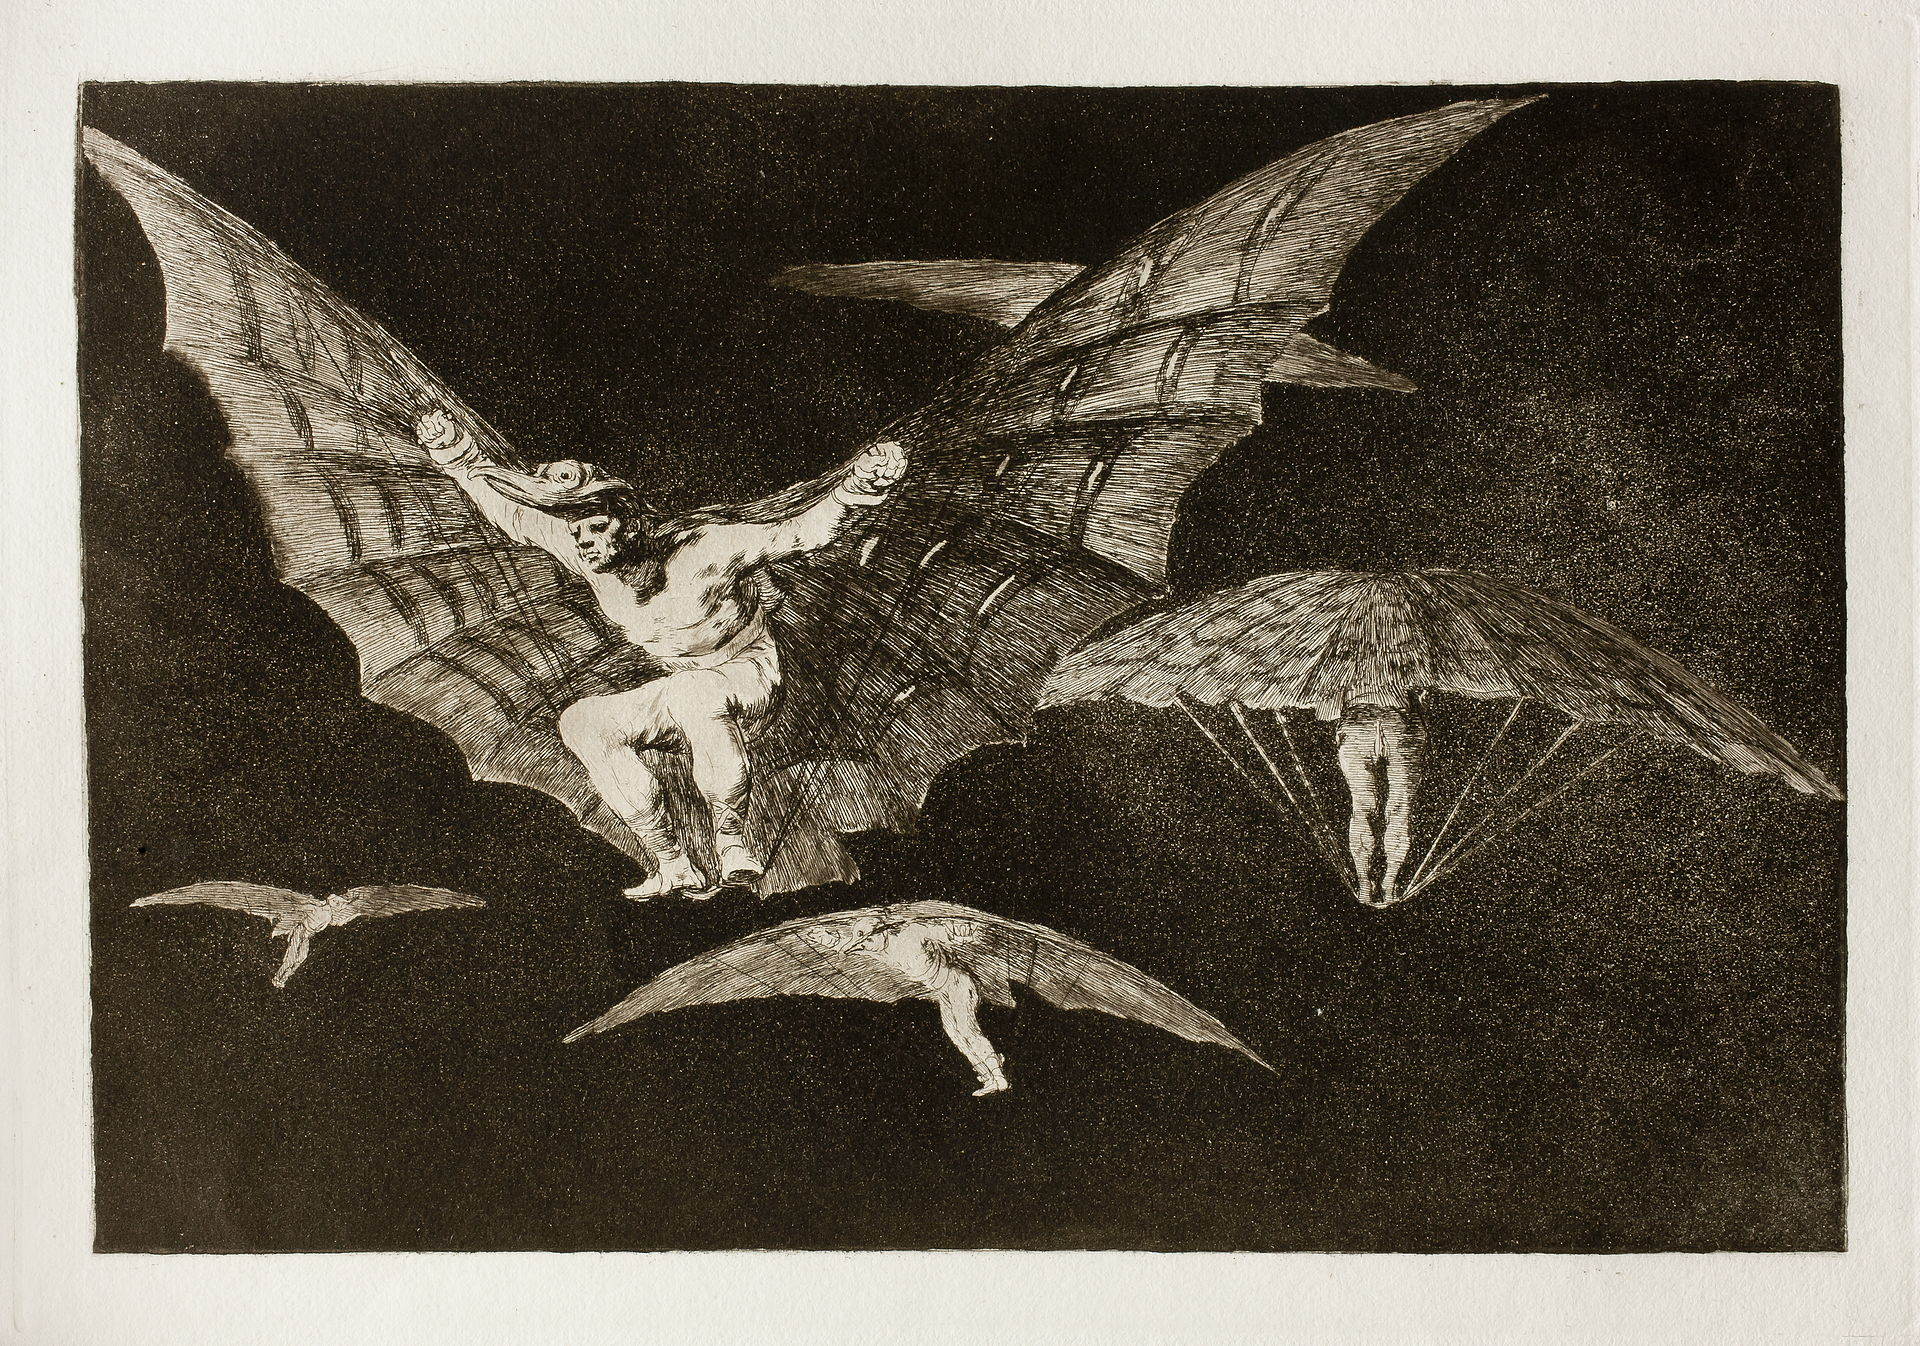
\includegraphics[width=1
		\textwidth]{goya-Modo_de_volar}
	\caption{``A way of flying'', Francisco Goya, 1815--1820, Amsterdam, Rijksmuseum.}\label{fig:goya} \end{figure}

They did not die in vain\footnote{Those ``researchers'' deserved a Darwin Award of science. The Darwin Award is satirical honours that recognise individuals who have unwillingly contributed to human evolution by selecting themselves out of the gene pool.}; Science advances when scientists are wrong. Theories must be falsifiable, and scientists cheer for their failure. When it fails, there is room for new approaches. Only when we understood the observations in animal flight from the perspective of aerodynamics, we learned to fly better than any other animal before. Science works by a ``natural selection'' of ideas, where only the fittest ones survive until a better one is born. Chaitin also points out that an idea has ``fertility'' to the extent to which it ``illuminate us, and inspires us with other ideas and suggests unsuspected connections and new viewpoints''~\cite[p. 9]{chaitin:2006}.\footnote{Moacir: and pass their gene on to children (possibly new better ones)?}\footnote{Moacir: did not get the analogy which is in the side note. }

Being a Babylonian enterprise, science has no clear path. One of the exciting facts one can learn by studying the history of science is that the most robust discoveries have arisen through the study of phenomena in human-made devices~\cite{pierce:1980}. For instance, Carnot's first and only scientific work\cite{klein:1974} gave birth to thermodynamics, which is the science that explains how steam engines work. However, steam engines came before Carnot's work and were studied by him\footnote{Moacir: please mention what was the nature and importance of his work in order for the reader to link heat engines with them.}~\cite{pierce:1980}. Thus, such human-made devices may present a simplified, small instance of more complex natural phenomena.

Another example is Information Theory. Several insights of Shannon's theory of communication were generalisations of ideas that were already present in Telegraphy. New theories in artificial intelligence can, therefore,  be developed from insights in the study of deep learning phenomena\footnote{Understanding human intelligence using artificial intelligence is a field of study called Computational Neuroscience.}.


\subsection{Bringing science to Computer Science} Despite the name, Computer Science has been more mathematics than science. We, computer scientists, are very comfortable with theorems and proofs, not much with theories.

Nevertheless, Artificial Intelligence (AI) has essentially become a Babylonian enterprise, a scientific endeavour. Thus, there is no surprise when some computer scientists still see AI with some distrust and even disdain:
\begin{itemize}
	\item Even among AI researchers, there is a trend of ``mathiness'' and speculation disguised as explanations in conference papers~\cite{lipton:2018}.
	\item There is no place for papers that unpretentiously describe surprising phenomena without trying to come up with an explanation. As if the mere inconsistency of the current theoretical framework was unworthy of publication.
\end{itemize}

While physicists rejoice in finding phenomena that contradict current theories, computer scientists get baffled. In Natural Sciences, unexplained phenomena lead to theoretical development. In AI, they bring ``winters'', periods of progress stagnation and lack of funding.\footnote{Moacir: not sure if I get this. Did you mean when some line of research is frozen until some new evidence flourishes?}.\index{ai winter}


\section{Problem}

\subsection{Has machine learning become alchemy?} Artificial Intelligence has been through several of the aforementioned ``winters''.  In 1957, Herbert Simon\footnote{Herbert Simon (1916--2001) received the Turing Award in 1975, and the Nobel Prize in Economics in 1978} famously predicted that within ten years, a computer would be a chess champion~\cite[section 1.3]{russell:2010}. It took around 40 years, in any case. Computer scientists lacked understanding of the exponential nature of the problems they were trying to solve: Computational Complexity Theory had yet to be invented.

Machine Learning Theory (computational and statistical) tries to avoid a similar trap by analysing and classifying learning problems according to the number of samples required to learn them (and the number of steps also). An honest assessment concludes it is now failing its mission. If by one hand, it leads to the development of practical machine learning algorithms like \acfp{SVM}\footnote{Moacir: define.}, by the other, it has also predicted that generalisation requires simpler models in terms of parameters, possibly delaying the development of Deep Learning for years\footnote{Moacir: other people would argue the development of DL was delayed by - lack of massive annotated data, lack of computational power, memory to handle such data}. In total disregard to the theory, deep learning models have shown spectacular generalisation power\footnote{Moacir: yes, for some domains/tasks, but even more spectacular capability of overfitting - even random labels} with hundreds of millions of parameters.

% \begin{quote}
% 	\small \textit{\flushright The curse of dimensionality is quite meaningless in practice[\ldots]\cite{howard:2018ml1}.\flushright --- Jeremy Howard, \spacedlowsmallcaps{fast.ai} creator\\
% 		\vspace{1cm} }
% \end{quote}

In the last decade, we have witnessed a myriad of astonishing successes in Deep Learning. Despite those many successes in research and industry applications, we may again be climbing a peak of inflated expectations. If, in the past, the false solution was to throw computation power on problems, today we try throwing data\footnote{Moacir: maybe both. Many SOA models are currently using ensembles of deep networks... but I get your point! in addition to the computational power, data is used in the same sense to draw conclusions that may not be reliable.}. Such behaviour has triggered a winner-takes-all competition among a handful of large corporations for who owns more data (our data), raising ethical concerns about privacy and concentration of power\cite{oneil:2016}\footnote{Moacir: maybe citing O'neil, weapons of Math Destruction or other work-related.}.

Nevertheless, we know that learning from way fewer samples is possible: humans show a much better generalisation ability than our current state of the art artificial intelligence. To achieve such needed generalisation power, we may need to understand better how learning happens in deep learning. Rethinking generalisation~\cite{zhang:2016} might reshape the foundations of machine learning theory.

\subsection{Problem statement} The practice of modern machine learning has outpaced its theoretical development. In particular, deep learning models present generalisation capabilities unpredicted by the current machine learning theory. There is yet no established new general theory of learning which handles this problem.

In 2015, Naftali Tishby and Noga Zaslavsky published a theory of learning based on the information-theoretical concept of the bottleneck principle~\cite{tishby:2015dlib}.

% This theory is general and can explain several deep learning phenomena inconsistent with the current Machine Learning Theory. The reason it is still not yet \textit{hors concours} is three-fold:
% \begin{enumerate}
% 	\item There has been some valid criticism to the experimental setting of the article mentioned above, which independent developments from~\citeauthor{achille:2017emergence}~\citeauthoritle{achille:2017emergence} address\footnote{Moacir: address?}.
% 	\item The understanding of this new theory demands prior knowledge in Information Theory to which deep learning practitioners of today are not used.
% 	\item Efforts on this new theory are scattered, and knowledge still needs to be consolidated.
% \end{enumerate}


\section{Objective}

This document aims to investigate the scattered efforts of using the information bottleneck principle to explain the generalisation capabilities of deep neural networks and consolidate them into a comprehensive digest of this new general deep learning theory.

Investigar até que ponto  IBT pode ajudar a melhor entender o Deep Learning e seus fenômenos; apresentando pontos fortes, fracos e oportunidades de pesquisa.

Perguntas de Pesquisa:
- Quais são os fundamentos da IBT? Como se diferem dos da MLT?
- É possível criar uma ponte entre MLT e IT através de IBT? Como IBT é diferente de abordagens anteriores nesse sentido como MDL?
- IBT invalida algum resultado de MLT?
- Pode IBT explicar fênomenos ainda pouco compreendidos?

Perguntas:
Quais são os fundamentos da IBT? Como se diferem dos da MLT?
É possível criar uma ponte entre MLT e IT através de IBT? Como IBT é diferente de abordagens anteriores nesse sentido como MDL?
Metodologia:
Derivar a partir de uma definição de inteligência tanto MLT, quanto IBT e identificar diferenças de  suposições.
Resultados Esperados:
Uma “árvore genealógica” das duas teorias e quadro comparativo.
Demonstração do conceito “fator de Occam” da perspectiva Bayesiana como sendo uma medida de informação.
Comparação IBT vs. MDL

Perguntas:
IBT invalida algum resultado de MLT?
Pode IBT explicar fênomenos ainda pouco compreendidos?
Metodologia:
A partir de uma lista de fenômenos compreendidos e não compreendidos, apontar diferenças entre a perspectiva atual e a da IBT.
Resultados Esperados:
As explicações correntes de MLT continuam válidas em IBT;
IBT pode explicar alguns aspectos de fenômenos ainda mal compreendidos.



\section{Outline}

The dissertation is organised in two parts:\\
PART I - Background:
\begin{itemize}
	\item Chapter 2--Artificial Intelligence: The chapter defines what artificial intelligence is, presents the epistemological differences of intelligent agents in history, and discusses their consequences to machine learning theory.
	\item Chapter 3 --- Probability Theory: The chapter derives propositional calculus and probability theory from a list of desired characteristics for sceptical agents.
	\item Chapter 4 --- Information Theory: The chapter derives Shannon Information from Probability Theory, explicates some implicit assumptions, and explains basic Information Theory concepts.
	\item Chapter 5 --- Machine Learning Theory: The chapter presents the theoretical framework of Machine Learning, the PAC model, theoretical guarantees for generalisation, and expose criticism due to its lack of explanation on Deep Learning phenomena.
	\item Chapter 6 --- Proposal: The chapter presents the plan for finishing the dissertation.
\end{itemize}

PART II --- An Information Theory of Deep Learning
\begin{itemize}
	\item Chapter 5 - The plan: In wich we present a plan to the dissertation.
 \end{itemize}

\begin{fullwidth}
\cleardoublepage \part{Background}\label{pt:background}
\end{fullwidth}
%************************************************
\chapter{Artificial Intelligence}\label{ch:artificial_intelligence}

%************************************************
\openepigraph{I visualize a time when we will be to robots
what dogs are to humans,$\ldots$ \\$\ldots$ and I’m rooting for the machines.}{Claude Shannon}

This chapter defines artificial intelligence, presents the epistemological differences of intelligent agents in history, and discusses their consequences to machine learning theory.


\section{Artificial Intelligence}
\begin{definition}
	\textbf{AI} is the branch of Computer Science that studies general principles of intelligent agents and how to construct them~\cite{russell:2010}.
\end{definition}
This definition uses the terms \emph{intelligence} and \emph{intelligent agents}, so let us start from them.

\subsection{What is intelligence?} Despite a long history of research, there is still no consensual definition of intelligence\footnote{For a list with 70 definitions of intelligence, see~\citeonly{legg:2007}.}. Whatever it is, though, humans are particularly proud of it. We even call our species \emph{homo sapiens}, as intelligence was an intrinsic human characteristic.

In this dissertation:
\begin{definition}
	\textbf{Intelligence} is the ability to predict a course of action to achieve success in specific goals.
\end{definition}

\subsection{Intelligent Agents} Under our generous definition, intelligence is not limited to humans. It applies to any agent\footnote{An agent is anything that perceives its environment and acts on it.}: animal or machine. A bacteria can perceive its environment through chemical signals, process them, and then produce chemicals to signal other bacteria. An air-conditioning can observe temperature changes, know its state, and adapt its functioning, turning off if it is cold or on if it is hot. \emph{Intelligence exempts understanding}. The air-conditioning does not comprehend what it is doing. The same way a calculator does not know arithmetics.

\subsection{A strange inversion of reasoning}\index{Daniel Dennet}\index{Strange inversion}\index{Turing}\index{Darwin}\index{Robert MacKenzie}

This competence without comprehension is what the philosopher Daniel Dennett calls \emph{Turing's strange inversion of reasoning}\label{turing_strange_inversion}. The a idea of a \emph{strange inversion} comes from one of Darwin's 19\textsuperscript{th} century critics (\citeauthor{mackenzie:1868} as cited by~\citeauthor{dennett:2009}):
\begin{quote}
	\small \emph{In the theory with which we have to deal, Absolute Ignorance is the artificer; so that we may enunciate as the fundamental principle of the whole system, that, \textbf{in order to make a perfect and beautiful machine, it is not requisite to know how to make it}. This proposition will be found, on careful examination, to express, in condensed form, the essential purport of the [Evolution] Theory, and to express in a few words all Mr Darwin's meaning; who, by \textbf{a strange inversion of reasoning}, seems to think Absolute Ignorance fully qualified to take the place of Absolute Wisdom in all of the achievements of creative skill.} \flushright{} --- Robert MacKenzie\\
\end{quote}
As counter-intuitive it was for~\citeauthor{mackenzie:1868} and many others to this date, intelligence can emerge from absolute ignorance. Turing's\footnote{Moacir: at least a side note on Turing's work or a reference.} strange inversion of reasoning comes from the realisation that his automata can perform calculations by symbol manipulation, proving that it is possible to build agents that behave intelligently, even if they are entirely ignorant of the meaning of what they are doing\footnote{As Harnard well observes in~\citeonly{turing:2007}, Turing in his on work discusses if computers can ``think'', meaning to discuss if they can be able to perform indistinguishably from the way thinkers do.}

\section{Dreaming of robots}

\subsection{From mythology to Logic}
The idea of creating an intelligent agent is perhaps as old as humans. There are accounts of what we call artificial intelligence in almost any ancient mythology: Greek, Etruscan, Egyptian, Hindu, Chinese~\cite{mayor:2018}. For example, in Greek mythology, the story of the bronze automaton of Talos built by Hephaestus, the god of invention and blacksmithing, first mentioned around 700 BC.\index{Mythology}

This interest may explain why, since ancient times, philosophers have looked for \emph{mechanical} methods of reasoning. Chinese, Indian and Greek philosophers all developed formal deduction in the first millennium BC.\@ In particular, Aristotelian syllogism, \emph{laws of thought}, provided patterns for argument structures to yield irrefutable conclusions, given correct premises. These ancient developments were the beginning of the field we call \emph{Logic}.\index{Logic}

\subsection{Rationalism: The Cartesian view of the world}

In the 13\textsuperscript{th} century, the Catalan philosopher Ramon Lull wanted to produce all statements the human mind can think. For this task, he developed ``logic paper machines'', discs of paper filled with esoteric coloured diagrams that connected symbols representing statements.\index{Ramon Lull}
\sidefigure{ars_magna_disc}{0}{Example of one of Lull's Ars Magna's paper discs.}
Unfortunately, according to~\citeauthor{gardner:1959},  in a modern reassessment of his work \textit{``it is impossible, perhaps, to avoid a strong sense of anticlimax''}~\cite{gardner:1959}. His delusional sense of importance, with megalomaniac self-esteem that hints at psychosis, is more characteristic of cult founders. On the bright side, his ideas and books exerted some magic appeal that helped them to be rapidly disseminated through all Europe~\cite{gardner:1959}.

Lull's work greatly influenced Leibniz and Descartes, who, in the 17\textsuperscript{th}century, believed that all rational thought could be mechanised. This belief was the basis of \textbf{rationalism}, the epistemic view of the \emph{Enlightment}, that regarded reason as the sole source of knowledge. In other words, they believed that reality has a logical structure and that certain truths are \emph{self-evidence}, and all truths can be derived from them.\index{Leibniz}\index{Descartes}

There was considerable interest in developing artificial languages during this period. Nowadays, they are called formal languages.
\begin{quotation}
	\small \emph{If controversies were to arise, there would be no more need for disputation between two philosophers than between two accountants. For it would suffice to take their pencils in their hands, to sit down to their slates, and to say to each other: \textbf{Let us calculate.}}\\
	\flushright --- Gottfried Leibniz\index{Leibniz}
\end{quotation}

The rationalist view of the world has had an enduring impact on society until today. In the 19\textsuperscript{th} century, George Boole and others developed a precise notation for statements about all kinds of objects in the world and the relations among them. Before them, Logic was philosophical rather than mathematical. The name of Boole's masterpiece, \emph{``The Laws of Thought''}, is an excellent indicator of his Cartesian worldview.

At the beginning of the 20\textsuperscript{th} century, some of the most famous mathematicians, David Hilbert, Bertrand Russel, Alfred Whitehead, were still interested in formalism: they wanted mathematics to be formulated on a solid and complete logical foundation. In particular, Hilbert's \textit{Entscheidungs Problem} (decision problem) asked if there were limits to the power of mechanical Logic proofs\cite{chaitin:2006}.

Kurt Gödel's incompleteness theorem (1931) proved that any language expressive enough to describe arithmetics of the natural numbers is either incomplete or inconsistent. This theorem imposes a limit on logic systems. There will always be truths that will not be provable from within such languages: i.e.\ there are true statements that are undecidable.

Alan Turing brought a new perspective to the \textit{Entscheidungs Problem}: a function on natural numbers that cannot be represented by an algorithm in a formal language cannot be computable\cite{chaitin:2006}. Gödel's limit appears in this context as functions that are not computable, e.g.\ no algorithm can decide whether another algorithm will stop or not (the halting problem). To prove that, Turing developed a whole new general theory of computation: what is computable and how to compute it, laying out a blueprint to build computers, and making possible the research of Artificial Intelligence as we know it. An area in which Turing himself was very much invested.

\subsection{Empiricism: The skeptical view of the world}
\sidefigure{hume}{0}{David Hume, Scottish Enlightenment philosopher, historian, economist, librarian and essayist.}

The response to \textbf{rationalism} was \textbf{empiricism}, the epistemological view that knowledge comes from sensory experience, our perceptions of the world. Locke explains this with the peripatetic axiom\footnote{This is the principle from the Peripatetic school of Greek philosophy and is found in Thomas Aquinas' work cited by Locke. }: \emph{``there is nothing in the intellect that was not previously in the senses''}\cite{williams:2020}. Bacon, Locke and Hume were great exponents of this movement, which established the grounds of the scientific method.

David Hume, in particular, presented in 18\textsuperscript{th} century a radical empiricist view: reason only does not lead to knowledge. In~\cite{hume:2009}, Hume distinguishes \emph{relations of ideas}, propositions which derive from deduction, and \emph{matters of facts}, which rely on the connection of cause and effect through experience, induction. Hume's critiques, known as \emph{the Problem of Induction}, added a new slant on the debate of the scientific method

From Hume's own words:
\begin{quotation}
	\small \emph{The bread, which I formerly eat, nourished me; that is, a body of such sensible qualities was, at that time, endued with such secret powers: but does it follow, that other bread must also nourish me at another time, and that like sensible qualities must always be attended with like secret powers? The consequence seems nowise necessary.} \flushright --- David Hume
\end{quotation}

There is no logic to deduce that the future will resemble the past. Still, we expect uniformity in Nature. As we see more examples of something happening, it is \emph{wise} to expect that it will happen in the future just as it did in the past. There is, however, no \emph{rationality} in this expectation.

Hume explains that we see conjunction repeatedly, \eg{} ``bread'' and ``nourish'', and we expect \emph{uniformity in Nature}, we expect that ``nourish'' will always follow ``eating bread''; When we fulfil this expectancy, we misinterpret it as causation. In other words, we \emph{project} causation into phenomena. Hume explicated that this connection does not exist in Nature. We do not ``see causation''; we create it.

This projection is \emph{Hume's strange inversion of reasoning}~\cite{huebner:2017}: We do not like sugar because it is sweet; Sweetness exists because we like (or need) it. There is no sweetness in honey. We wire our brain so that glucose triggers a labelled desire we call sweetness. As we will see later, sweetness is \emph{information}. This insight shows the pattern matching nature of humans. Musicians have relied on this for centuries. Music is a sequence of sounds in which we expect a pattern. The expectancy is the tension we feel while the chords progress. When the progression finally \emph{resolves}, forming a pattern, we release the tension. We feel pattern matching in our core. It is very human, it can be beneficial and wise, but it is, stricto sensu, \emph{irrational}\footnote{Moacir: says who?}.

The epistemology of the sceptical view of the world is science: to weigh one's beliefs to the evidence. Knowledge is not absolute truth but justified belief. It is a Babylonian epistemology.

In rationalism, Logic connects knowledge and good actions. In empiricism, the connection between knowledge and justifiable actions is determined by probability. More specifically, by Bayes' theorem\footnote{The Bayes' theorem is attributed to the Reverend Thomas Bayes after the posthumous publication of his work. By the publication time, it was an already known theorem, derived by Laplace.}. As Jaynes puts it, probability theory is the Logic of Science~\cite{jaynes:2003}.
\subsection{The birth of AI as a research field}
\sidefigure{shannon}{0}{Claude Shannon, father of ``information theory''.}

In 1943, McCulloch and Pitts, a neurophysiologist and a logician, demonstrated that neuron-like electronic units could be wired together, act and interact by physiologically plausible principles and perform complex logical calculation~\cite{russell:2010}. Moreover, they showed that any computable function could be computed by some network of connected neurons~\cite{mcculloch:1943}. Their work marks the birth of \acfp{ANN}, even before the field of AI had this name. It was also the birth of \textbf{Connectionism}, the approach of using artificial neural networks, loosely inspired by biology, to explain mental phenomena and imitate intelligence.

Their work was an inspiration to John von Neumann's demonstration on how a universal Turing machine can be created out of electronic components, which lead to the advent of computers and programming languages. Ironically, these advents hastened the ascent of the formal logicist approach called \textbf{Symbolism}, disregarding Connectionism.\index{John von Neumann}\index{Claude Shannon}

In 1956, John McCarthy, Claude Shannon (who invented Information Theory, \cref{fig:shannon}), Marvin Minsky and Nathaniel Rochester organised a 2-month summer workshop in Dartmouth College to bring researchers of different fields concerned with \emph{``thinking machines''} (cybernetics, information theory, automata theory). The workshop attendees became a community of researchers, and the term \emph{``artificial intelligence''} was chosen for the field.
\section{Building Intelligent Agents}
% \blockfigure{elephant}{0}{The Blind Men and the Elephant.}
% \begin{quotation}
% 	\centering \small \emph{ It was six men of Indostan\\
% 	To learning much inclined,\\
% 	Who went to see the Elephant\\
% 	(Though all of them were blind),\\
% 	That each by observation\\
% 	Might satisfy his mind\\
% 	\flushright{} ---John Godfrey Saxe, The Blind Men and the Elephant~\cite{saxe:2016}\label{blind_men}\\
% 	}
% \end{quotation}
\subsection{Anatomy of intelligent agents}\label{sec:anatomy_ia}

Like the blind men in the parable, an intelligent agent shall model her understanding of the world\footnote{We are using the word \emph{world} as in~\citeonly{sowinski:2016}, to denote \emph{environment} or \emph{Nature}.} from limited sensory data.
\blockfigure{anatomy}{0}{Anatomy of an Intelligent Agent. Inspired by art in\protect{~\citeonly{russell:2010}}.}


Thus, an agent perceives her world with sensors, treat sensory data as facts and use these facts to possibly update its model of the world, use the model to decide her actions, and acts via her actuators. In a way, agents continually communicate with the world in a perception/action conversation (\cref{fig:anatomy}).

The expected result of this conversation is a change in the agent's \acf{KB}, therefore in her model and, more importantly, her future decisions. The model is an abstraction of how the agent ``thinks'' the world is (her ``mental picture'' of the environment). Therefore, it should be consistent with it: if something is true in the world, it is equally true, \emph{mutatis mutandis}, in the model. A Model should also be as simple as it can be such that the agent can make decisions that maximise a chosen performance measure, but not simpler. As the agent knows more about the world, less it gets surprised by it.

This rudimentary anatomy is flexible enough to entail different epistemic views, like the rationalist (mathematical) and the empirical (scientific); different approaches to how to implement the knowledge base (it can be learned, therefore updatable, or it can be set in stone from an expert prior knowledge); and also from how to implement it (a robot or a software).

Noteworthy, though, is that the model that transforms input data into decisions should be the target of our focus.

\subsection{Symbolism} Symbolism is the pinnacle of rationalism. In the words of Thomas Hobbes, one of the forerunners of rationalism, \emph{``thinking is the manipulation of symbols and reasoning is computation''.} Symbolism is the approach to building intelligent agents that does just that. It attempts to represent knowledge with a formal language and explicitly connects the knowledge with actions. It is \emph{competence from comprehension}. In other words, it is \emph{programmed}.

Even though McCulloch and Pitts work on artificial neural networks predates Von Neumann's computers and the increase of interest in the study of \emph{``thinking machines''} of the 1950s that would become AI, Symbolism dominated the field until the 1980s. It was so ubiquitous that nowadays, symbolic AI is even called ``good old fashioned AI''\cite{russell:2010}.

The symbolic approach can be traced back to Nichomachean Ethics~\cite{aristotle:2000}:
\begin{quotation}

	\small \emph{
		We deliberate not about ends but means. For a doctor does not deliberate whether he shall heal, nor an orator whether he shall persuade, nor a statesman whether he shall produce law and order, nor does anyone else deliberate about his end. They assume the end and consider how and by what means it is to be attained; and if it seems to be produced by several means, they consider by which it is most easily and best produced, while if it is achieved by one only they consider how it will be achieved by this and by what means this will be achieved, till they come to the first cause, which in the order of discovery is last.
		}

	\flushright{} --- Aristotle\
\end{quotation}

This perspective is so entrenched that~\citeauthor[p. 7]{russell:2010} still says: \emph{``only by understanding how actions can be justified can we understand how to build an agent whose actions are justifiable''}; even though, in the same book, they cover machine learning (which we will address later in this chapter) without noticing it is a proof that there are other ways to build intelligent agents. Moreover, it is also a negation of competence without comprehension. The reality is that even for many AI researchers, the strange inversion of reasoning is uncomfortable. All humans, even those in prisons and under mental health care, think their actions are justifiable. Is that not an indication that we rationalise our actions post factum?

\subsubsection{Claude Shannon’s Theseus}\index{Claude Shannon}
After writing what is probably the most important master's dissertation of the 20\textsuperscript{th} century and ``inventing'' the Information Theory that made possible the Information Age we live in today, Claude Shannon enjoyed the freedom to pursue any interest to which his curious mind led him~\cite{soni:2017}. In the 1950s, his interest shifted to building artificial intelligence. He was not a typical academic, in any case. A lifelong tinkerer, he liked to ``think'' with his hand as much as with his mind. Besides developing an algorithm to play chess (when he even did not have a computer to run it), one of his most outstanding achievements in AI was Theseus, a robotic maze-solving mouse\footnote{Many AI students will recognise in Theseus the inspiration to Russel and Norvig's Wumpus world~\cite{russel:2010}.}.

To be more accurate, Theseus was just a bar magnet covered with a sculpted wooden mouse with copper whiskers; the maze was the ``brain'' that solved itself.
\begin{quote}
	\small \emph{``Under the maze, an electromagnet mounted on a motor-­powered carriage can move north, south, east, and west; as it moves, so does Theseus. Each time its copper whiskers touch one of the metal walls and complete the electric circuit, two things happen. First, the corresponding relay circuit's switch flips from ``on'' to ``off,'' recording that space as having a wall on that side. Then Theseus rotates \(90^{\circ}\) clockwise and moves forward. In this way, it systematically moves through the maze until it reaches the target, recording the exits and walls for each square it passes through.\flushright{} ---~\citeauthor{klein:2018}''}.
\end{quote}
\subsubsection{Symbolic AI problems} Several symbolic AI projects sought to hard-code knowledge about domains in formal languages, but it has always been a costly and slow process that could not be scaled.

Anyhow, by $1965$ there were already programs that could solve any solvable problem described in logical notation~\cite[p.4]{russell:2010}. However, hubris and lack of philosophical perspective made computer scientists believe that ``intelligence was a problem about to be solved\footnote{Marvin Minsky, head of the artificial intelligence laboratory at MIT ($1967$)}.''

Those inflated expectations lead to disillusionment and funding cuts~\cite{russel:2010}. They failed to estimate the inherent difficulty in slating informal knowledge in formal terms: the world has many shades of grey. Besides, complexity theory had yet to be developed: they did not count on the exponential explosion of the problems with which they were dealing.

\subsection{Connectionism: a different approach}

Connectionism is an approach to the study of human cognition that utilizes mathematical models, known as connectionist networks or artificial neural networks. It was pioneered by McCulloch and Pitts in 1943~\cite{mcculloch:1943}. One of the most famous developments of the first wave of connectionism was Frank Rosenblatt's Perceptron, an algorithm for learning binary classifiers, or more specifically threshold functions:
\begin{align}
	y=
	\begin{cases}
		1 \text{ if } \mW\vx + \vb > 0\\
		0 \text{ otherwise }
	\end{cases}
\end{align}
where \(\mW \) is the vector of weights, \(\vx \) is the input vector, \(\vb \) is a bias and \(\vy \) is the classification. In the context of neural networks, a perceptron is an artificial neuron using a step function as the activation function.

The fundamental idea in Connectionism is that \textbf{intelligent behaviour emerges from a large number of simple computational units when networked together}~\cite{goodfellow:2016}.
\begin{figure}
	[hbt!] \centering
	\begin{sidecaption}[Biomimicry of termite technique achieves superior energy efficiency in buildings]{Biomimicry of termite technique achieves superior energy efficiency in buildings.}
	\begin{subfigure}
		[b]{.4
		\textwidth} \centering
		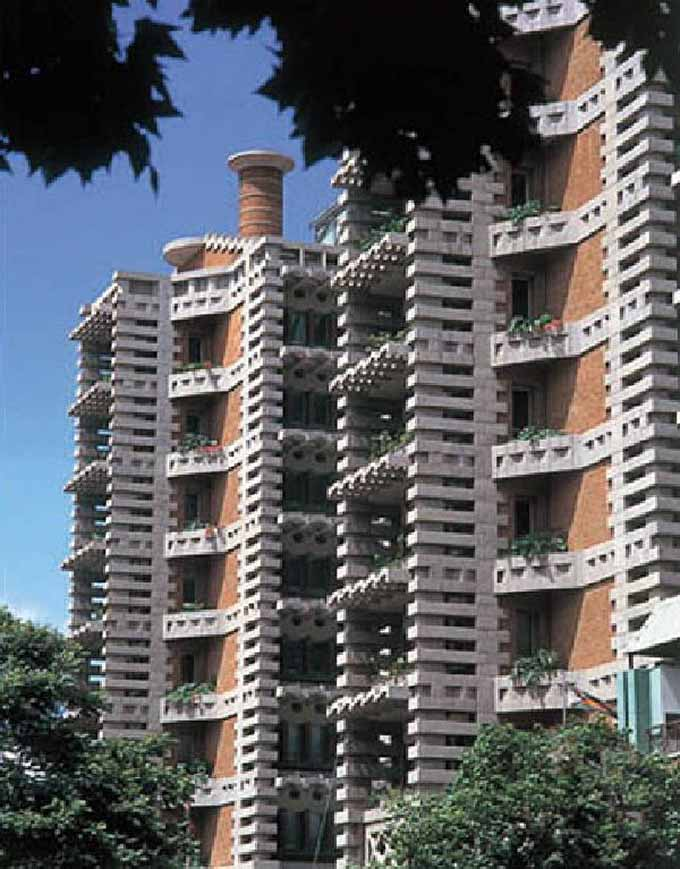
\includegraphics[width=.9
		\textwidth]{arup_building}
		\caption*{Building in Harare, Zimbabwe is modelled after termite mounds. Photo by Mike Pearce.}\label{fig:arup_building} \end{subfigure}
	\hspace*{1em}
	\begin{subfigure}
		[b]{.35
		\textwidth} \centering
		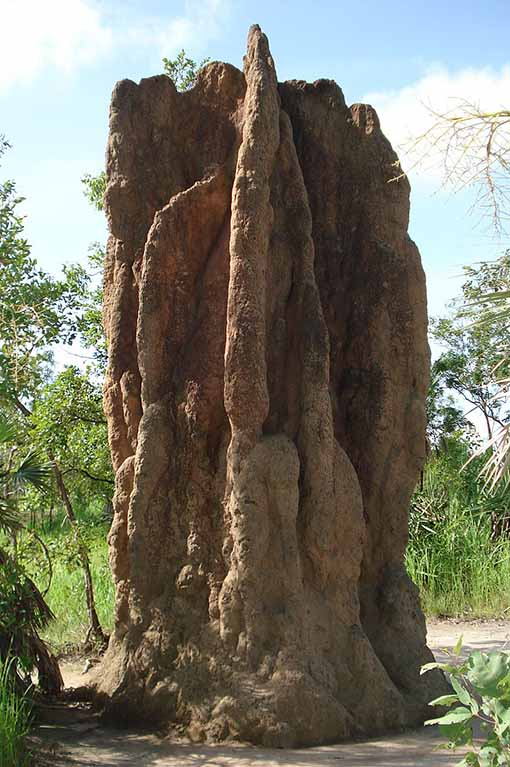
\includegraphics [width=.9
		\textwidth]{termite_cathedral}
		\caption*{Cathedral termite mound, Australia. Photo by Awoisoak Kaosiowa, 2008.}\label{fig:termite_cathedral} \end{subfigure}
	\end{sidecaption}\label{fig:termites}
\end{figure}

See \cref{fig:termites}, termites self-cooling mounds keep the temperature inside at exactly \(31^{\circ} C\), ideal for their fungus-farming; while the temperatures outside range from 2 to \(40^{\circ} C\) through the day. Such building techniques inspired architect Mike Pearce to design a shopping mall in Zimbabwe that uses a tenth of the energy used by a conventional building of the same size.

From where does termites intelligence come?
\begin{quotation}
	\small \emph{Individual termites react rather than think, but at a group level, they exhibit a kind of cognition and awareness of their surroundings. Similarly, in the brain, individual neurons do not think, but thinking arises in their connections.}\flushright{} --- Radhika Nagpal, Harvard University~\cite{margonelli:2016}.
\end{quotation}

Such collective intelligence happens in groups of just a couple of million termites. There are around 80 to 90 billion neurons in the human brain, each one of them less capable than a termite, but collectively they show still uncomparable intelligence capabilities.

\begin{figure}
	[ht!] \centering
	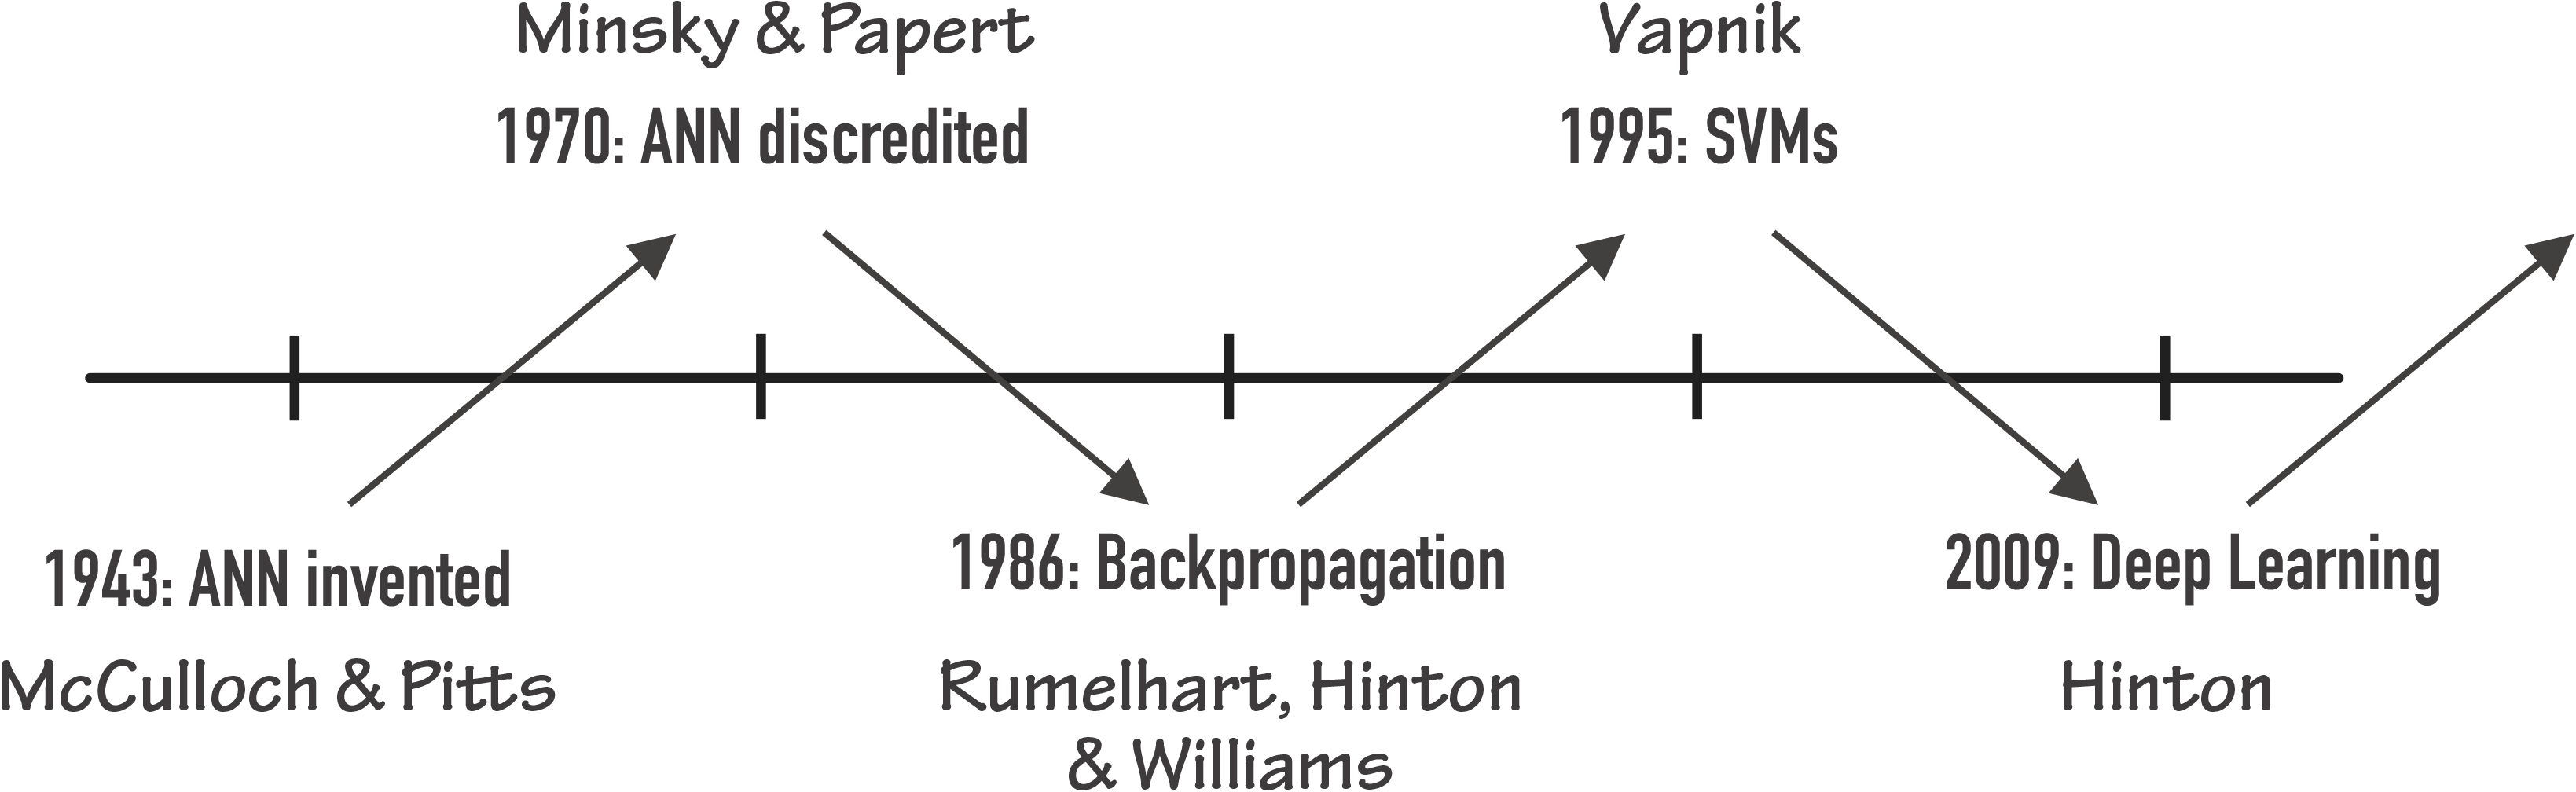
\includegraphics[width=0.8
	\textwidth]{winters}
	\caption{A brief history of connectionism. Inspired by~\citeonly{tishby:2020DeepMath}.}\label{fig:connectionism}
\end{figure}
In contrast with the symbolic approach, in neural networks, the knowledge is not explicit in symbols but implicit in the strength of the connections between the neurons. Besides, it is a very general and flexible approach since these connections can be updated algorithmically: they are algorithms that \emph{learn}: the connectionist approach is an example of what we now call Machine Learning.


\subsection{Machine Learning}
\sidefigure{lulu}{0}{Is this a cat?}

Look at the \cref{fig:lulu}. Is this a picture of a cat? How to write a program to do such a simple classification task (cat/no cat)? One could develop clever ways to use \emph{features} from the input picture and process them to make a guess. Though, it is not an easy program to design. Worse, even if one manages to program such a task, how much would it worth to accomplish a related task, to recognise a dog, for example?

For a long, this was the problem of researchers in many areas of interest of AI:\@ \acf{CV}, \acf{NLP}, Speech Recognition; much mental effort was put, with inferior results, in problems that we humans solve with ease.

The solution is an entirely different approach for building artificial intelligence: instead of building the program to do the task, build the program that outputs the program that does the task. In other words, learning algorithms use what we call ``training data'' to infer the transformations to the input that generates the desired output. It is competence without comprehension.

\subsubsection{Types of learning} Machine Learning can happen in different scenarios, which differ in the availability of training data, how training data is received, and how the test data is used to evaluate the learning. Here, we describe the most typical of them~\cite{mohri:2012}:
\begin{itemize}
	\item \textbf{Supervised learning:} The most successful scenario. The learner receives a set of labelled examples as training data and makes predictions for unseen data.
	\item \textbf{Unsupervised learning:} The learner receives unlabeled training data and makes predictions for unseen instances.
	\item \textbf{Semi-supervised learning:} The learner receives a training sample consisting of both labelled and unlabelled data and makes predictions for unseen examples. Semi-supervised learning is usual in settings where unlabeled data is easily accessible, but labelling is too costly.
	\item \textbf{Reinforcement learning:} The learner actively interacts with the environment and receives an immediate reward for her actions. The training and testing phases are intermixed.
\end{itemize}

\subsection{Deep Learning} The \(2010_s\) have been an AI Renaissance not only in academia but also in the industry. Almost all the successes are due to \acf{DL}, in particular, supervised deep learning with vast amounts of data trained in \acfp{GPU}. It was the decade of \ac{DL}.

\emph{``Deep learning algorithms seek to exploit the unknown structure in the input distribution to discover good representations, often at multiple levels, with higher-level learned features defined in terms of lower-level features~\citeauthor{bengio:2012}}''.The name is explained by one of his students~\cite{goodfellow:2016}: ``\emph{A graph showing the concepts being built on top of each other is a deep graph. Therefore the name, deep learning}''. Although it is a direct descendant of the connectionist movement, it goes beyond the neuroscientific perspective in its modern form. It is more a general principle of learning multiple levels of compositions.

The quintessential example of a deep learning model is the deep feedforward network or \acf{MLP}~\cite{russell:2010}.
\begin{figure}[hbt!]
	\begin{neuralnetwork}
		[height=4]
		\newcommand{\x}[2]{\(x_#2\)}
		\newcommand{\y}[2]{\(\hat{y}_#2\)}
		\newcommand{\hfirst}[2]{\small \(h^{(1)}_#2\)}
		\newcommand{\hsecond}[2]{\small \(h^{(2)}_#2\)} \inputlayer[count=3, bias=true, title=Input\\layer, text=\x] \hiddenlayer[count=4, bias=false, title=Hidden\\layer 1, text=\hfirst] \linklayers \hiddenlayer[count=3, bias=false, title=Hidden\\layer 2, text=\hsecond] \linklayers \outputlayer[count=2, title=Output\\layer, text=\y] \linklayers
	\end{neuralnetwork}
	\end{figure}
\begin{definition}
	Let,
	\begin{itemize}
		[leftmargin=1.5cm]
		\item [\(\vx\)] be the input vector \(\{\vx_1, \ldots, \vx_m\}\)
		\item[\(k\)] be the layer index, such that \(k \in [1,l] \),
		\item[\(d_k\)] is the number of elements in the hidden layer \({(k)}\),
		\item[\(\mW^{(k)}_{i,j}\)] be the matrix of weights in the \(k\)-th layer, where \( i \in [0,d_{k-1}], j \in [1, d_k] \text{ and }\mW^{(k)}_{0,:}\) are the biases
		\item[\(\sigma~\)] be a non-linear function,
	\end{itemize}
	a \textbf{\acfp{MLP}} is a neural network where the input is defined by:
	\begin{align}
		h^{(0)}= 1^\frown \vx,
	\end{align}
	a hidden layer is defined by:
	\begin{align}
		h^{(k)}&=\sigma^{(k)}(\mW^{(k)~\top} h^{(k-1)}).
	\end{align}
	The output is defined by:
	\begin{align}
		\hat{y}&=h^{(l)}.
	\end{align}
\end{definition}


Deep Learning is usually associated with \acfp{DNN}, but the network architecture is only one of its components:
\begin{enumerate}
	\item DNN architecture
	\item \acf{SGD} --- the optimiser
	\item Dataset
	\item Loss function
\end{enumerate}

The architecture is not the sole component essential to current Deep Learning success. The \ac{SGD} plays a crucial role, and so does the usage of large datasets.

A known problem, though, is that DNNs are prone to overfitting (\cref{sec:bias-variance}). ~\citeauthor{zhang:2016} shows that state-of-the-art convolutional deep neural networks can easily fit a random labelling of training data.

%************************************************
\chapter{Probability Theory}\label{ch:probability}

%************************************************
\begin{quotation}
	\small \emph{ \flushright A wise man proportions his belief to the evidence.\\
	\flushright --- David Hume\\
	\vspace{1cm} }
\end{quotation}

In this chapter, propositional calculus and probability theory are derived from a list of desired characteristics for sceptical agents.

\section{From Language to Probability}\label{sec:language_probability}
\subsection{Formal Languages} We, as intelligent agents, do not know how the World is; we only know how we perceive it. Our ideas are mental pictures of how we imagine the World. Like in the story of the blind men and the elephant (\cref{blind_men}), how do we know that our model is the same as someone else's? \emph{Communicating}. We need to communicate with each other to check if our mental picture of the World, our model, is consistent with the experience of others.\footnote{We can take this idea further and think that at any moment we need to communicate with our past selfs to check if new evidence is consistent with our prior model.}.

We use language to describe the World. However, natural languages, like English, German, Portuguese, are ambiguous, and we need contextual clues and other information to more clearly communicate meaning. To avoid this, an intelligent agent uses formal language.

A formal language is a mathematical tool created for precise communication about a specific subject. For example, arithmetic is a language for calculations. Chemists have a language that represents chemical structures of molecules. Programming languages are formal languages that express computations. In a nutshell, a formal language is a set of words (strings) whose letters (symbols) are taken from an alphabet and are well-formed according to a specific set of rules, a grammar:
\begin{align}
	\text{Let }\lang&= <\Sigma, \Phi>,~\text{be a formal language where:}\\
	\Sigma &= \{S_1, S_2, \cdots, S_n\} \text{ is an alphabet,}\\
	\Phi &= {\Phi_1 \cup \Phi_2 \cup \cdots \cup \Phi_k} \text{ is a set of operations,}
\end{align}
where:
\begin{align}
	\Phi_1 &\text{ is the set of unary operations}, \nonumber\\
	\Phi_2 &\text{ is the set of binary operations}, \nonumber\\
	\cdots &\nonumber \\
	\Phi_k &\text{ is the set of k-ary operations}\nonumber
\end{align}
A formal language allows a quantitative description of a state of knowledge and defines how this state can be updated on new evidence.

With this definition, we can also think that a formal language is what~\citeauthor{sowinski:2016} calls a \emph{realm of discourse}, \ie all the valid formed \emph{strings}\footnote{Strings, words, sentences, propositions, formulae are names used interchangeably through the literature.} that one can derive; everything one can \emph{say} about the world.

Interestingly, formal languages allow us to manipulate representations of the world without dealing with their semantics. They are the basis of \emph{``Turing's strange inversion''}, (see \cref{turing_strange_inversion}) by doing allowed operations on strings, computers can compute at a superhuman speed and accuracy without ever comprehending what they are doing.

\subsection{From Rationalism to Propositional Calculus}
\paragraph{Rational Agents} Rational agents are agents that can form representations of a complex world, use deduction as the inference process to derive updated representations, and use these new representations to decide what to do. In other words, rational agents are the consequence of the epistemological view of \emph{rationalism}.

When a particular statement's truth value is established by a rational agent, all statements formed in her knowledge base from that statement instantly feel that update. A rational agent cannot hold contradictions.

\paragraph{Desiderata for a rational language}\label{sec:desiderata_language}

We want to build a language for rational agents with the following desired characteristics:
\begin{enumerate}
	[I.]
	\item \textbf{knowledge is absolute}; a sentence\footnote{A sentence can be either a single symbol or a string formed with several symbols according to the grammar.} can be either true or false;
	\item \textbf{unambiguous}, a constructed sentence can only have one meaning;
	\item \textbf{consistent}; a language without paradoxes, \ie whatever path chosen to derive a sentence truth value will lead to the same assignment;
	\item \textbf{minimal}; uses the smallest set of symbols possible.
\end{enumerate}

Let \(\lang_R= <\Sigma_R, \Phi_R>\) be the formal language built from these constraints; where sentences are either axiom symbols or compounded sentences formed using special symbols called operators, each operator denoting one operation \(\phi \in \Phi_R\).

It is possible to prove\label{future:prove_minimal_language_logic} that \(\lang_R\) only needs one operator~\cite{sowinski:2016,jaynes:2003}: \spacedlowsmallcaps{nand} (or \spacedlowsmallcaps{xor}), and it is also equivalent to Propositional Calculus.\footnote{Proposition is synonym to sentence, and Propositional Calculus is also known as Sentential Calculus.}.~\label{insert_appendix} In other words, Logic is the language that emerges from our desiderata, from rationalism. \textbf{Logic is the language of mathematics}.

A point worth mentioning is that using Logic as an agent formal language means the \textbf{implicit acceptance} of the constraints above.

\subsection{From Empiricism to Probability Theory}

The constraints that lead to Logic are very restrictive to use in the real world; the rational language has a comparatively small realm of discourse. Hume would say that it is only helpful for \emph{relations of ideas}, talking in the abstract, and not for \emph{matters of facts}, talking about reality.

A realm of discourse to talk about reality needs at least the empiricist perspective where knowledge is justified belief, and that one should \emph{weights her beliefs to the evidence.} The quantity that specifies to what degree we believe a proposition is true is constrained by other beliefs, i.e.\ by previous experience and evidence gathering.

\paragraph{Sceptical Agents}\label{sec:sceptical_agent}\label{sec:sceptical_agents} In the sceptical agent derived from the empiricist epistemology
(authors have called these agents epistemic agents~\cite{caticha:2008}, idealised epistemic agents~\cite{sowinski:2016} or robots~\cite{jaynes:2003}), beliefs are not independent of each other~\cite{caticha:2008}, they form an interconnected web that is the agent's knowledge base. The update mechanism, its inference method, follows the principle of minimality, i.e.\ it tries to minimise the change in the knowledge base.

\paragraph{Desiderata for a sceptical language} As we did for rational agents, let us state a set of desired characteristics for the language of Science, \(\lang_S= <\Sigma_S, \Phi_S>\)
% \footnote{~\cite{sowinski:2016,caticha:2008, jaynes:2003} also present this same idea of deriving probability theory from a desiderata.}:
\begin{enumerate}[I.]
	\item \textbf{Knowledge is a set of beliefs, quantifiable by real numbers and dependent on prior evidence:~\cite{sowinski:2016,caticha:2008, jaynes:2003}}\footnote{Moacir: is this yours formulation?} \\
	Let \(S_i \in \Sigma_S\) be sentences about the world. Given any two statements \(S_1\), \(S_2\), the agent must be able to say that \(S_1\) is more plausible than \(S_2\), or that \(S_2\) is more plausible than \(S_1\), or that \(S_1\) and \(S_2\) are equally plausible~\cite{caticha:2008}. Thus we can list statements in an increasing plausibility order. Real numbers can represent this transitive ordering~\cite{caticha:2008}.\footnote{We are implicitly assuming that the language we are building has infinite statements. A further discussion on this continuity assumption can be found in~\cite[p. 26]{sowinski:2016}}.

	Let \(b\) be a measure of degrees of belief in \(S\) given some previous knowledge \(K\):\footnote{Moacir: K --- is it an (observable) event? or knowledge/axiom?}
	\footnote{Using \((S|K)\) in a function is a notation abuse that we accept in order to better explain the idea.}:
	\begin{align}
		b: \Sigma_S \to \Real\\
		b: S \mapsto b(S|K)
	\end{align}
	Here we capture the fact that plausibility (degrees of belief) is not a function of a sentence, but a relation between a sentence and a given assumed prior knowledge.
	\item \textbf{``Common sense:''}\\
	The plausibility of compound sentences should be related by some logical function to the plausibility of the sentences that form them. \\
	We already showed that a minimal rational language has only one operator. Here, instead of using the \spacedlowsmallcaps{nand} operator, for a matter of familiarity, let us use the almost minimal language with the operators \spacedlowsmallcaps{not} (\(\neg\)) and \spacedlowsmallcaps{and} ($\land$). In this setting, we are saying there are such functions $f$ and $g$ that~\cite{sowinski:2016}:
	\begin{enumerate}[(a)]
		\item \(b(\neg S|K) = f[b(S|K)]\)
		\item \(b(S_1 \land S_2 | K) =\\g[b(S_1|K), b(S_1|S_2), b(S_2|K), b(S_2|S_1)]\)
	\end{enumerate}
	\item \textbf{Consistency:}\\
	The functions \(f\) and \(g\) must be consistent with the grammar \(\Phi\) (production rules).\\Consistency guarantees that whatever path used to compute the plausibility of a statement in the context of the same knowledge web (the same set of constraints) must lead to the same degree of belief.\label{consistency}
	\begin{enumerate}
		[(a)]
		\item Beliefs that depend on multiple propositions cannot depend on the order in which they are presented.\label{axiom:order}
		\item No proposition can be arbitrarily ignored.
		\item Propositions which are known to be identical must be assigned the same degree of belief.
	\end{enumerate}
\end{enumerate}
\sidefigure{kolmogorov}{-20}{Andrey Kolmogorov, Soviet mathematician.}

Such desiderata have a name; it is known as Cox's axioms, and one can derive the Sum Rule and the Product Rule (see \cref{sec:probability}) from them, therefore, also the Bayes' Theorem (\cref{sec:bayes_theorem}), and reverse-engineer Kolmogorov's Axioms of Probability Theory (\cref{sec:kolmogorov_axioms}, \cref{fig:kolmogorov})\label{future:cox_to_kolmogorov}~\cite{sowinski:2016, jaynes:2003, caticha:2008, terenin:2015}.

In other words, Probability Theory is the language that emerges from our desiderata, from empiricism. \textbf{Probability theory is the logic of science}~\cite{jaynes:2003}, and our measure \(b\) is what is usually called probability~\(P\).

Again, here we explicit that by using Bayesian inference to build and communicate concepts of the world (models), we are assuming Cox's axioms above.

\subsection{Assumptions and their consequences} As a side note, let us take this opportunity to explore what some assumptions mean to human intelligence in particular. It is indisputable\footnote{Unless you are an economist.} that humans are not rational, neither sceptical agents. The whole idea of imagining a sceptical agent is a consequence of wanting to address intelligence without the human complexities.

However, are humans irrational because of biology or psychology? Are we irrational for lack of will, or could it be that Nature wires the human brain in a way that pr\emph{events} us from following these axioms? Here we argue that biology has an important role. Researchers have found, for instance, that visual acuity can be permanently impaired if there is a sensory deficit during early post-natal development~\cite{wiesel:1982}. If the human brain is not exposed to some samples in its infancy, it will never achieve the accuracy level it could achieve if it had experienced them, regardless of experiencing those examples later. In other words, \emph{human beliefs depend on the order in which pieces of evidence are presented}, contradicting Cox's axiom~\ref{axiom:order}.


\section{Formalizing Probability Theory} Up to this point in the chapter, our purpose was to give an intuition of what probability is. We did that by showing that it is possible to derive Kolmogorov's Axioms (\cref{sec:kolmogorov_axioms}) from the empiricist epistemology. In this section, we will use these axioms to derive concepts in Probability Theory.

Worth of mention, several concepts in this section are \emph{relations of ideas}, not \emph{matters of fact}. The probability of an \emph{event} E, P(E), can be computed by marginalisation (see Subsection~\ref{marginalisation}), but as discussed before, there are no beliefs in a vacuum. In reality, there is only the probability of an \emph{event} E given some background knowledge \(K\). This change of epistemological perspective is essential to be remembered now; that we will expose the idealised development of concepts in Probability Theory.


\section{Experiments, Sample Spaces and Events}

The set of possible outcomes of an \textbf{\emph{experiment}} is the \textbf{sample space} \(\Omega\). Let us use the canonical \emph{experiment} of rolling a dice. In this experiment, the sample space is:
\begin{align*}
	\Omega = \left\{\epsdice{1},\epsdice{2},\epsdice{3},\epsdice{4},\epsdice{5},\epsdice{6} \right\}
\end{align*}
An \textbf{outcome} or \textbf{realization} is a point $\omega \in \Omega$:
\begin{align*}
	\omega_3&=\epsdice{3}\\
	\Omega &= \left\{\omega_1=\epsdice{1},\cdots,\omega_6=\epsdice{6} \right\}.
\end{align*}
An \textbf{Event} is something you can say about the \emph{experiment}, \eg ``The dice rolled to the an odd number''. It is a true proposition. But easier than writing so much, we denote \emph{events} with letters. \textbf{Events are subsets of \(\Omega\)} (see \cref{fig:event_A}).
\begin{align*}
	A &= \left\{\va_1=\epsdice{1}, \va_2=\epsdice{3}, \va_3=\epsdice{5} \right\}\\
	A &\subset \Omega
\end{align*}
We say that $A_1, A_2, \cdots$ are \textbf{mutually exclusive} or \textbf{disjoint} \emph{events} if $A_i \cap A_j=\emptyset, \forall i\neq j$. For example, \(A\) is the \emph{event} ``the dice rolled to the value 5'' and \(B\) is the \emph{event} ``the dice rolled to an even number''. In this case, \(A\) and \(B\) are disjoint (see~\cref{fig:disjoint_events})
\begin{figure}
	[hbt!] \centering
	\begin{subfigure}
		[t]{.3
		\textwidth} \centering
		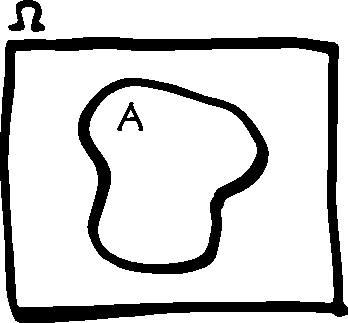
\includegraphics[width=3cm]{eventA}
		\caption{An \emph{event} \(A\).}\label{fig:event_A}
	\end{subfigure}
		\hfill
	\begin{subfigure}
			[t]{.3
			\textwidth} \centering
			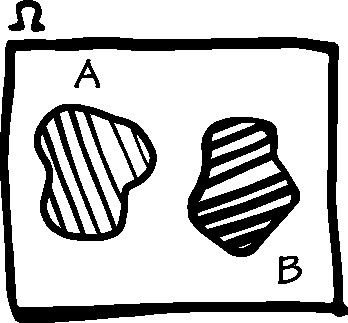
\includegraphics[width=3cm]{disjointAB}
			\caption{Disjoint events \(A\) and \(B\): \(A \cap B = \emptyset\).}\label{fig:disjoint_events}
	\end{subfigure}
	\hfill
	\begin{subfigure}
		[t]{.3
		\textwidth} \centering
		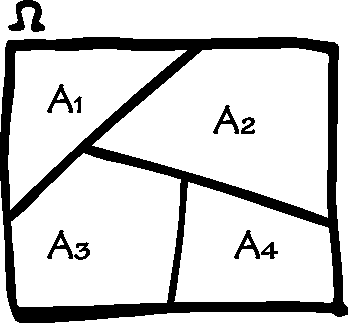
\includegraphics[width=3cm]{partition}
		\caption{A partition of \(\Omega\):\\
		\(\bigcup\limits_{i}^{} A_i = \Omega\).}\label{fig:partition}
	\end{subfigure}
	\caption{Events, disjoint events and partitions.}
\end{figure}
A \textbf{partition} of $\Omega$ is a sequence of disjoint events (sets) \(A_i\) (see~\cref{fig:partition}), where:
\begin{align}
	A_1, A_2, \cdots A_i \text{ s.t. } (A_1 \cup A_2 \cup A_3 \cdots = \bigcup\limits_{i=1}^{\infty} A_i) = \Omega
\end{align}


\section{Probability}\label{sec:probability}
\marginnote{The powerset of \(\Omega\), \(\powerset(\Omega)\), is the set of all possible subsets of \(\Omega\).}
\begin{definition}[Kolmogorov's Axioms]\label{sec:kolmogorov_axioms}
	A function \(P: \powerset(\Omega) \to \sR \) that maps any \emph{event} \(A\) to a real number \(P(A)\) is called the \textbf{probability measure} or a \textbf{probability distribution} if it satisfies the Kolmogorov's axioms~\cite{wasserman:2013}:
	\begin{enumerate}[\textbf{Axiom} 1., leftmargin=3cm]
		\item \(P(A)\geq 0, \forall A\)
		\item \(P(\Omega)=1\)
		% \item If \(A\) and \(B\) are disjoint, i.e. \(A \ind B \),\label{axiom:disjoint}
		\begin{align}
			P(A \lor B)= P(A)+P(B)\label{eq:sum_rule} \\
			\nonumber \tag{Sum Rule}
		\end{align}
	\end{enumerate}
\end{definition}

Visually, we can represent the probability of an \emph{event} \(A\), \(P(A)\), as the proportion of the sample space, the \emph{event} occupies. To diferentiate \emph{events} from their probabilities, we will shade the area of the \emph{event}.
\begin{figure}[ht!]
\captionsetup[subfigure]{labelformat=empty}
\begin{sidecaption}[Kolmogorov's Axioms and their direct consequences.]{Kolmogorov's Axioms and their direct consequences.}\label{fig:kolmogorov_axioms}
\centering
\begin{subfigure}[t]{.3\textwidth}\centering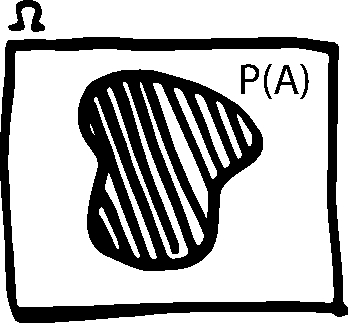
\includegraphics[width=3cm]{pA.pdf}
	\caption{Axiom 1: \\\(P(A)\geq 0\)}\label{fig:axiom1}
\end{subfigure}
\hfill
\begin{subfigure}[t]{.3\textwidth} \centering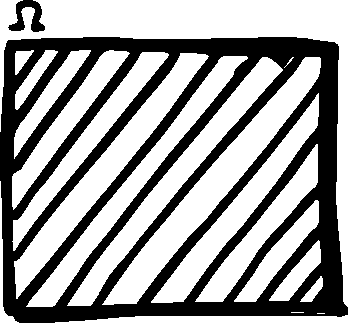
\includegraphics[width=3cm]{p1}
	\caption{Axiom 2:\\\(P(\Omega)=1\).}\label{fig:axiom2}
\end{subfigure}
\hfill
\begin{subfigure}[t]{.3\textwidth} \centering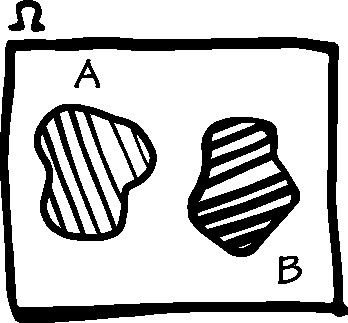
\includegraphics[width=3cm]{disjointAB}
	\caption{Axiom 3: \(A \cap B = \emptyset \implies P(A \lor B)=P(A)+P(B)\).}\label{fig:axiom3}
\end{subfigure}
\hfill
\begin{subfigure}
[t]{.3
\textwidth} \centering

\includegraphics[width=3cm]{emptyspace}
\caption{\(P(\emptyset)=0\).}
\end{subfigure}
\hfill
\begin{subfigure}
[t]{.3
\textwidth} \centering
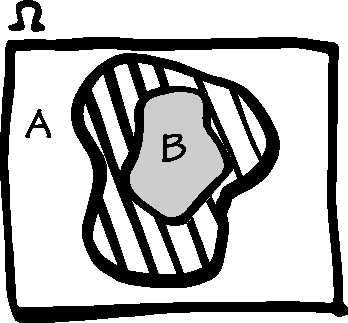
\includegraphics[width=3cm]{BinA}
\caption{\(B\subset A \to P(B) \leq P(A)\).}
\end{subfigure}
\hfill
\begin{subfigure}
[t]{.3
\textwidth} \centering
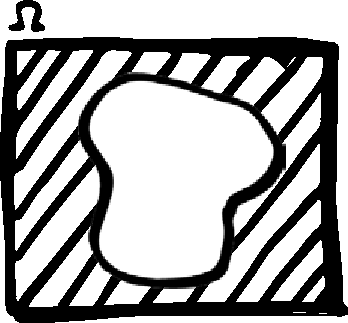
\includegraphics[width=3cm]{complementA}
\caption{\(P(\bar{A})=1-P(A)\).}
\end{subfigure}
\end{sidecaption}
\end{figure}

Directly from the Kolmogorov Axioms, one can derive~\cite{jaynes:2003} other properties (see \cref{fig:kolmogorov_axioms_derivations}):
\begin{align}
P(\emptyset)&=0\\
B \subset A &\implies P(B) \leq P(A)\\
0 &\leq P(A) \leq 1\\
P(\bar{A})&=1-P(A).
\end{align}



\section{Joint event}
\begin{definition}
A joint \emph{event} \(A, B\) is the set of outcomes where:
\[(A, B) = {\omega \in \Omega: (\omega \in A \cap B) } \]
Therefore,
\[P(A, B) =P({\omega \in \Omega: (\omega \in A \cap B) }) \]
\end{definition}
\marginnote{\vspace{-2cm}
\begin{align}
&P(A,B) &~\equiv~ &P(B,A)&~\equiv~ \nonumber\\
&P(A \land B)&~\equiv~ &P(A \cap B)&~\equiv~  \nonumber\\
&P(A \times B).\nonumber
\end{align}
}
When talking about \emph{events} as propositions, it is straightforward to use logic notation \(P(A \land B)\), but when we start to use \emph{random variables} (\cref{sec:random_variables}), we will adopt the shorthand notation \(P(\rvA, \rvB)\).
\sidefigure{joint_event}{0}{Joint event (A, B).}

\section{Independent events}\label{sec:independent_events}
\begin{definition}\label{def:independence}
Events \(A\) and \(B\) are \textbf{independent} (\(A \ind B\)) if:
\begin{align}
A\neq \emptyset, B\neq \emptyset \implies P(A)>0, P(B)>0\label{eq:P(A, B)>0}\\
P(A, B) = P(A \land B) = P(A) \cdot P(B)\label{eq:Product_Rule}\\
\nonumber \tag{Product Rule}
\end{align}
\end{definition}

\textbf{Disjoint \emph{events} cannot be independent}, since (from~\eqref{eq:P(A, B)>0}) \(P(A) \cdot P(B)> 0\), but as disjoint \emph{events} (\cref{fig:disjoint_events}) \(P(A \land B)=P(\emptyset)=0\), leading to contradiction.

Independence can be assumed or derived by verifying:
\begin{align}
P(A \land B)= P(A) \cdot P(B).\\
\nonumber \tag{Independent variables}
\end{align}


\section{Conditional probability}
\marginpar{
\centering
\begin{gather*}
P(A|B)=\frac{ 
\includegraphics[width=2cm]{eventAB} }
{ 
\includegraphics[width=2cm]{eventB}}
\end{gather*}
}
% \begin{wrapfigure}{R}{0.27\textwidth}
% 	\centering
% 	\begin{gather*}
% 		P(A|B)=\frac{ 
\includegraphics[width=2cm]{eventAB} }
% 		 						{ 
\includegraphics[width=2cm]{eventB}}
% 	\end{gather*}
% \end{wrapfigure}
As we have explained before (\cref{sec:sceptical_agent}), the plausibility of an outcome or a set of outcomes depends on a web of interconnected prior beliefs. So, in reality, as a \emph{matter of fact}, what exists are probabilities \emph{conditional} to a given prior assumption.

\begin{definition}
If \(P(B)>0\) then the \textbf{conditional probability} of A given B is:
\begin{align}\label{eq:conditional_probability}
P(A|B) \eqdef \frac{P(A,B)}{P(B)}
\end{align}
Also:
\begin{align}\label{eq:joint_probability}
P(A, B) \eqdef P(A|B)\cdot P(B)
\end{align}
\end{definition}


Except if \(P(A) \equiv P(B)\), \(P(A|B) \neq P(B|A)\). Also, \(P(A|B)=P(A) \iff A \ind B\).\footnote{Venn diagrams are not helpful to see that the \emph{events} are independent, as it all depends on the areas of intersection and the sizes of A and B, which are quite difficult to estimate without computational help.}.

\section{Marginal probability}\label{marginalisation}
\begin{theorem}
Let \(A_1, \cdots, A_k\) be a partition of \(\Omega\). Then, for any \emph{event} B,
\begin{align}
P(B)=\sum_{i=1}^k P(B|A_i)\cdot P(A_i)\label{eq:law_of_total_probabilities} \end{align}
\end{theorem}
\blockfigure{total_probability}{1}{An \emph{event} B, a partition \(A_i\) over \(\Omega\), and \(C_i = (B, A_i) \).}

\begin{proof}
\footnote{Remember: \((B, A) \equiv (B \cap A)\).}
Define \(C_i = (B,A_i)\). Let \(C_1, \cdots C_k\) be disjoint and \(B = \bigcup\limits_{i=1}^k C_i\). \\
Therefore:

	\begin{align}
		P(B) &\triangleq P(\bigcup\limits_{i=1}^k C_i)
		\overset{\text{\ref{eq:sum_rule}}}{=} \sum_i P(C_i)\\
		&\triangleq \sum_i P(B,A_i)
		\overset{\text{\ref{eq:conditional_probability}}}{=} \sum_{i=1}^k P(B|A_i)\cdot P(A_i) \tag{Law of Total Probability}
	\end{align}
\end{proof}
\section{Bayes' theorem}\label{sec:bayes_theorem}
\begin{theorem}
	Let \(A_1, \cdots, A_k\) be a partition of \(\Omega\) s.t. \(P(A_i)>0, \forall i\) then, \(\forall i=1, \cdots, k\):
	\begin{align}
		P(A_i|B)= \frac{P(B|A_i)\cdot P(A_i)}{\sum_i P(B|A_i)\cdot P(A_i)} \tag{Bayes' theorem}
	\end{align}
\end{theorem}
\begin{proof}
	From equations~\ref{eq:conditional_probability},~\ref{eq:joint_probability} and~\ref{eq:law_of_total_probabilities}:
	\begin{align}
		P(A_i|B)&\overset{\text{\ref{eq:conditional_probability}}}{=}\frac{P(A_i,B)}{P(B)} \overset{\text{\ref{eq:joint_probability}}}{=} \frac{P(B|A_i) \cdot P(A_i)}{P(B)}  \\
		&\overset{\text{\ref{eq:law_of_total_probabilities}}}{=}\frac{P(B|A_i)\cdot P(A_i)}{\sum_{i=1}^k P(B|A_i)\cdot P(A_i)}
	\end{align}
\end{proof}
We call \(P(A_i)\) the \textbf{prior} of A, and \(P(A_i|B)\) the \textbf{posterior} probability of A.
\section{Random variables}\label{sec:random_variables}
\begin{definition}
	A \textbf{random variable} is a mapping \(\rvX:\Omega \to \Real\) that assigns a real number \(\rvX(\omega)\) to each outcome \(\omega\), \(\omega \mapsto \rvX(\omega)\).
\end{definition}
\blockfigure{random_variable}{0}{Random variable.}

Given a random variable \(\rvX\), the probability of an outcome \(\rx\) can be expressed as:
\begin{align}
	P(\rvX=\rx) = P(\rvX^{-1}(\rx)) = P(\{\omega \in \Omega: \rvX(\omega)=\rx\})\label{eq:P(X=x)} \end{align}

Several works on Probability Theory choose to start by defining random variables, rarely mentioning sample spaces, \emph{events} or the connection with logical propositions.

This usual approach is, nevertheless, confusing. Beyond the fact that random variables are not variables, but functions; nor random, they model uncertain \emph{events}; it is hard to grasp what random variables are without understanding their reasons for being.

% The difference between a random variable 𝑋 and a ``realization'' of it is the difference between a distribution and a sample from that distribution. In particular, a random variable 𝑋 is ``formalized'' in terms of a function from the sample space to some result space, typically 𝐑. The realization of a random variable is ``what you get'' when an \emph{experiment} is run, and you figure out which \emph{events} happened, and you apply 𝑋 to those \emph{events}.
%

\subsection{Notation hell} If a \emph{random variable} is a function, how can we write \(P(\rvX=4)\) or \(P(\rvX > 7)\)? The reason for such confusion is due to some notation abuse that became standard in works on probability theory. It is not easy to grasp it in the beginning, but the explanation was already stated at~\eqref{eq:P(X=x)}. \(P(\rvX=\rx)\) is a shorthand for \(P(\rvX^{-1}(\rx))\).

Technically, a \emph{random variable} is a function.  In practice, it is just a mathematical tool to help us associate propositions with numbers. It is called a \emph{random variable} because the notation abuse treats the function as a variable.

To help clear up such confusion, let us recap a little the notation we have established before:

In the canonical \emph{experiment} of rolling a dice, instead of writing the plausability of the proposition \emph{``The dice will roll to number 4''} is \(\frac{1}{6}\), it is easier to assign a letter to the proposition, or as we called the \emph{event}. Let us use \emph{event} \(D\) to represent the proposition. Then, we can use \(P(D)=\frac{1}{6}\). Now, we are going one step further, instead of using the \emph{event} \(D\) we use the \emph{random variable} \(\rvD\), in italic, and say \(P(\rvD=4)=\frac{1}{6}\).

Notice the difference between a \emph{random variable} and an \emph{event}
% .\footnote{An \emph{event} can be seen as a special kind of \emph{random variable}.  \Eg, a random variable \(\rvD\) is the truth function (also known as the indicator function) over an event \(D\):
% \begin{align*}
% 	\rvD=\truth_D
% \end{align*}
% That is the reason one can say that ``\emph{random variables} define \emph{events}.'' }
: \(\rvD\) could assume any value (even \(\rvD=7\) which is clearly outside of our \emph{sample space}). Would it not be easier then to use an index to the \emph{event} letters, \ie \(D_4\) to value 4, and \(D_1\) to value 1, etc.? Not really.

Besides providing this shorter notation, the mapping of the random variable allows us to manipulate \emph{events} as numbers: for example, we can chart probability distributions using random variables, which we cannot cope with \emph{events}.


\section{Probability Distributions}
\sidefigure{distribution}{0}{Probability mass function, probability density function, and probability of an interval (hatched area).}

\begin{definition}
	A probability distribution of a discrete random variable \(\rvX\) or \textbf{probability mass function (pmf)} is a function \(p: \Omega \to [0,1]\) that provides the probabilities of occurrence of different possible outcomes in an \emph{experiment} (sample space):

	\begin{align}
		p(\rx) = P(\rvX = \rx), \tag{pmf}
	\end{align}
\end{definition}

If \(\rvX\) is countinuous, \(P(\rvX=\rx)\to 0\), therefore we need to use intervals in this case.
\begin{definition}
	A probability distribution of a countinous random variable \(\rvX\) in an interval \(A\), or \textbf{probability density function (pdf)} is a function \(p(\rx)\) that measures the probability of randomly selecting a value within the interval \(A=[a, b]\), as the area under its curve for the interval A:\@
	\begin{flalign}
		P(A) &= P[a \leq \rvX \leq b] = \int_{a}^{b} p(\rx) \, d\rx, \text{ and:}\\
		&
		\begin{cases}
			p(\rx) \geq 0, \forall x \tag{pdf}\\
			\int\limits_{\Real}^{} p(\rx) \, d\rx = 1
		\end{cases}
	\end{flalign}
\end{definition}
Now that we explained what distributions are,\footnote{In this dissertation, we will use $P(\rvX)$ to express the probability of a random variable, and $p(\rx)$ to represent a \emph{pmf} or \emph{pdf} of the random variable outcomes.} here we highlight some useful distributions:
\subsection{Statistical model}\label{sec:statistical_model}
A statistical model is a function $p_{\theta}(\rx) \equiv p(\rx | \theta)$ that represents the relationship between a parameter\footnote{In this dissertation we are interested in vector-valued $\theta$.} $\theta$ and potential outcomes $\rx$ of a random variable $\rvX$. In practice, we normally define a statistical model of a stochastic process for which we do not the real distribution. Therefore, the parameter $\theta$ has to be inferred from the observed data.
\subsection{Uniform distribution}\label{sec:uniform_distribution}
\marginpar{
	\begin{minipage}{\marginparwidth}
		\centering
		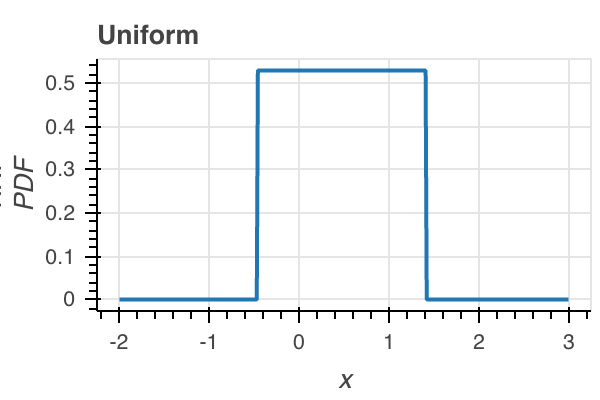
\includegraphics[width=0.9\textwidth]{uniform}
		\captionof{figure}{Uniform distribution.}\label{fig:uniform_distribution}
		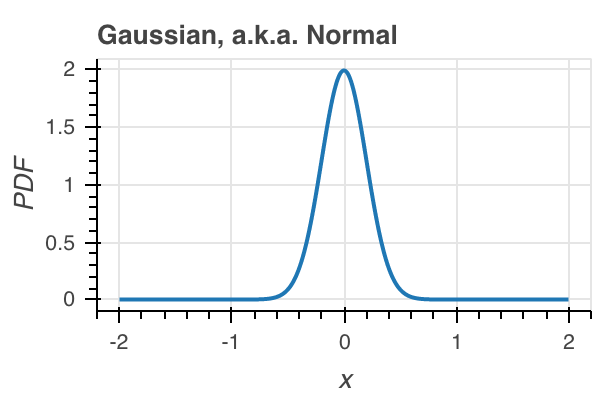
\includegraphics[width=0.9\textwidth]{gaussian}
		\captionof{figure}{Gaussian distribution, also known as the \emph{normal}.}\label{fig:gaussian_distribution}
		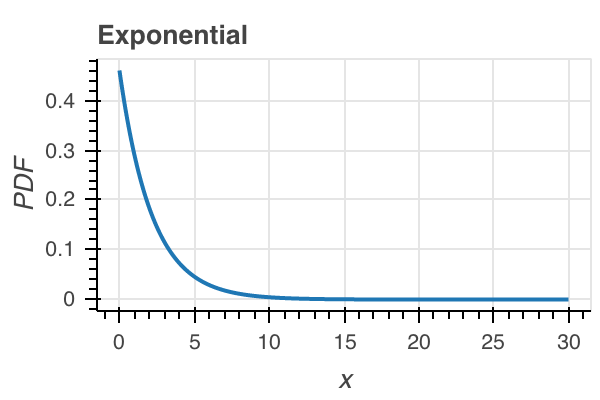
\includegraphics[width=0.9\textwidth]{exponential}
		\captionof{figure}{Exponential distribution.}\label{fig:exponential_distribution}
	\end{minipage}
}
\(\nonumber \\\rvX \sim \text{Uniform}(a,b)\), if:\\
\begin{align*}
	p(\rx)=
	\begin{cases}
		\frac{1}{b-a} & x \in [a,b]\\
		0 & \rx \notin [a,b]
	\end{cases}
\end{align*}
\subsection{Normal distribution}
\(\nonumber \\\rvX \sim N(\mu, \sigma^2)\), if:
\begin{align*}
	p(\rx)=\frac{1}{\sigma \sqrt{2\pi}}\exp{\Biggl{\{}{-\frac{1}{2\sigma^2}{(x-\mu)}^2}\Biggr{\}}}, \\~x \in \Real \\
\end{align*}
where \(\mu \in \Real\) (mean) and \(\sigma > 0\) (standard deviation). We say that \(\rvX\) has a \textbf{standard Normal distribution} if \(\mu = 0\), \( \sigma =1\).
\subsection{Exponential distribution}
\(\rvX \sim \text{Exp}(\lambda)\), if:
\begin{align*}
	p(\rx;\lambda) =
	\begin{cases}
		\lambda e^{-\lambda \rx} & \rx \ge 0, \\
		0 & \rx < 0.
	\end{cases}
\end{align*}
where \(\lambda > 0\) is the \emph{rate parameter} of the distribution.


\section{Joint Distributions}
\sidefigure{joint_distribution}{0}{A chart of a joint distribution.}

\begin{definition}
	Given a pair of discrete random variables \(\rvX\) and \(\rvY\), we define the \textbf{joint mass function} by \(p(\rx, \ry)=P(\rvX=\rx,\rvY=\ry)\).
\end{definition}
\begin{definition}
	Given a pair of continuous random variables \(\rvX\) and \(\rvY\), we define the \textbf{joint density function} by \(p(\rx, \ry)\), where:
	\begin{enumerate}
		[i.]
		\item \(p(\rx, \ry) \geq 0\)
		\item \(\bigintssss_{-\infty}^{\infty}\bigintssss_{-\infty}^{\infty}p(\rx,\ry) \, d\rx d\ry =1\)
		\item \(\forall A \subset \Real \times \Real, P((\rvX,\rvY)\in A)=\bigintssss\bigintssss_{A}p(\rx,\ry)\, d\rx d\ry \).
	\end{enumerate}
\end{definition}


\section{Expectancy, Variance and Covariance}
\begin{definition}
	The \textbf{expected value} or \textbf{mean} of \(\rvX\) is:
	\begin{align}
		\E (\rvX)=\langle \rvX \rangle = \SumInt_x \rx~p(\rx)~dx = \mu = \mu_X
	\end{align}
\end{definition}
\begin{theorem}
	Let \(\rvX_1, \cdots, \rvX_n\) be random variables and \(a_1, \cdots, a_n\) be constants, then from the \emph{Sum Rule}:
	\begin{align}
		\E \biggl(\sum_i a_i\rvX_i\biggr)=\sum_i a_i(\E (\rvX_i))
	\end{align}
\end{theorem}
\begin{theorem}
	Let \(\rvX_1, \cdots, \rvX_n\) be independent random variables, then from the \emph{Product Rule}:
	\begin{align}
		\E (\prod_i \rvX_i)=\prod_i \E (\rvX_i)
	\end{align}
\end{theorem}
\begin{definition}
	Let \(\rvX\) be a random variable with mean \(\mu\). The \textbf{variance} of \(\rvX\) is defined by:
	\begin{align}
		\sigma^2 = \sigma_{\rvX}^2 =\E {(\rvX - \mu)}^2
	\end{align}
	assumming this expectation exists. The standard deviation is \(\sigma\).
\end{definition}
\begin{definition}
	Let \({\rvX}\) and \({\rvY}\) be random variables with means \(\mu_{\rvX}\) and \(\mu_{\rvY}\), and with standard deviations \(\sigma_{\rvX}\) and \(\sigma_{\rvY}\). The \textbf{covariance} between \({\rvX}\) and \({\rvY}\) is defined as~\cite[p.74]{wasserman:2013}:
	\begin{align}
		\operatorname{Cov}({\rvX},{\rvY}) = \E (({\rvX} - \mu_{\rvX})({\rvY} - \mu_{\rvY}))
	\end{align}
	and the correlation as:
	\begin{align}
		\rho = \rho_{{\rvX},{\rvY}} = \rho({\rvX},{\rvY}) = \frac{\operatorname{Cov}({\rvX},{\rvY})}{\sigma_{\rvX} \sigma_{\rvY}}
	\end{align}
\end{definition}
\begin{theorem}
	The covariance satisfies:
	\begin{align}
		\operatorname{Cov}({\rvX},{\rvY})=\E ({\rvX}{\rvY})- \E({\rvX}) \E({\rvY}).
	\end{align}
\end{theorem}


\section{Independent Sampling}
% \begin{figure}[hbt!] \centering
% 	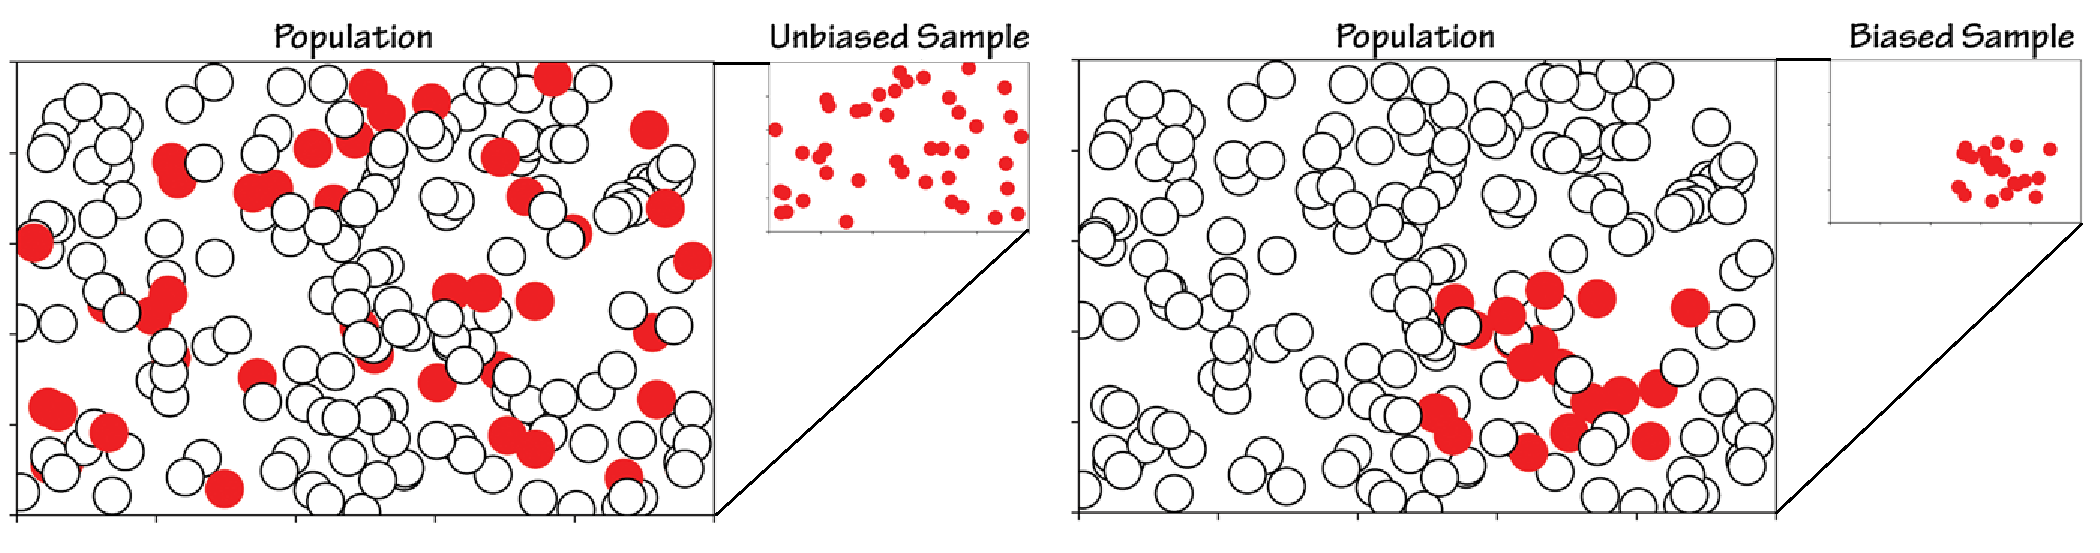
\includegraphics[width=
% 	\textwidth]{sampling2}
% 	% \caption{An i.i.d. sample (left) and a biased sample (right). Adapted from~\cite{mello:2018}.}\label{fig:sampling}
% \end{figure}
  A \emph{sample} is a set of examples drawn from a distribution.
One common assumption in Machine Learning Theory is that examples are \emph{identically and independently distributed --- i.i.d.} This means that the probability of obtaining a first training example
.\footnote{In this document, an element of a sampling is called an \emph{example}. } \((\rx_1, \ry_1)\) does not affect which \((\rx_2, \ry_2)\) will be draw in the next observation.

The i.i.d. assumption is useful wherever a census of the population of interest, knowing all possible values, is unfeasible. In this usual case, data analysis is carried out using a sample to represent the population. When the sample is i.i.d., each example in the population has the same chance of being observed (\cref{fig:sampling} --- left).

If there is a constraint on which examples of the population are sampled, we say that the sample is \emph{biased} (\cref{fig:sampling} --- right).

\section{Bibliographical Remarks}
Many essential topics in Statistics were left out from this short review chapter, where the focus was to present the concepts that we will later on in this dissertation.

Overall, the chapter was influenced by~\citeauthor{wasserman:2013}. The idea to derive Probability Theory from Logic can be found in~\citeauthor{jaynes:2003},~\citeauthor{sowinski:2016} and~\citeauthor{caticha:2008}, being this last resource one of the most complete in the subject.


% \subsection{Forward and inverse probabilities}

% % \paragraph Forward probabilities are used to describe a generative model that give rise to some data. They arise in problems where the task is to find out the probability distribution of some quantity produced by the process.
% % \paragraph Inverse probability problems also involve a generative model of a process, but instead of finding out the probability distribution of some quantity produced by the process, we want the conditional probability of one or more of the unobserved variables in the process, given the observed variables.
% % Given a probability distribution \(p(x|\theta)\) (the forward probability) for an observable quantity \(x\) conditional on an unobserved variable \(\theta \), the \emph{inverse probability} is the posterior distribution \(p(\theta|x)\), obtained by applying the Bayes' theorem.
% %
% %

% \subsection{Induction as inverse probability}

% % %
% %

% \subsection{Compression and inverse probability}


%************************************************
\chapter{Machine Learning Theory}\label{ch:mlt}

%************************************************
\openepigraph{Mathematics operates inside the thin layer
between the trivial and the intractable.}{Andrey Kolmogorov}

In which we present the theoretical framework of Machine Learning, the PAC model, theoretical guarantees for generalisation, and expose criticism due to its lack of explanation on Deep Learning phenomena\footnote{This chapter is influenced by the online lecture~\citeonly{shawe-taylor:2018}, the online lecture series~\citeonly{mello:2018online} and the book~\citeonly{mello:2018}. }.

\section{Motivation} As already discussed, learning is the process of inferring general rules to perform a specific task by observing limited examples. The learning algorithm must perform well in the sample already seen and, more importantly, in previously unseen examples.

How can we prove that an algorithm learned? We may know its performance in the given sample, but does it translate to any sample? Can we guarantee bounds to the error in an unknown distribution of examples even if we have just a limited sample of it? Can we bound the number of samples needed (sample complexity) to ensure accuracy on unseen examples? How does the sample complexity grow?
\sidefigure{vc}{0}{Chervonenkis (Left) and Vapnik (Right).}
These are the kind of questions that motivated the development of Machine Learning Theory (MLT). This research field started in Russia by the name of Statistical Learning Theory (SLT), during the late \(1960_s\), with the work of Vapnik and Chervonenkis (see \cref{fig:VC}). In 1984, Leslie Valiant proposed the Probably Approximately Correct (PAC) framework to bring ideas from the Computational Complexity Theory to learning problems, giving birth to the field of Computational Learning Theory (CoLT). Up to the \(1990_s\), STL and CoLT were very active fields.
We will also limit our overview of MLT to the context of supervised binary classification problems. This limitation is not a deficiency of the theory but a mere choice of scope for this document.


\section {The Learning Problem}
The goal of learning is to understand the world from experience, coming up with a theory, a tested hypothesis.
\sidefigure{concept}{0}{A \emph{concept} \(c\) is an idealised mapping from the input space \(\XX\) to output space \(\YY\). Each point on the left is an instance \(\rx_i\). Note that given that \(\YY\) is binary, \(c \subset \XX\).}

The learning task is the \emph{concept} \(c\) we want to learn. The concept is the idealised function that maps an instance of the problem \(\rx_i\) from the input space \(\XX\) (also known as problem space) to a solution \(\ry_i\) of the output space \(\YY\) (also known as label space). In the PAC framework, the convention is that labels are binary, \(\YY = \{-, +\}\), therefore, \(c \subset \XX\). A concept class \(\CC\) is a set of concepts \(c\), thus, a set of sets of \(\XX\).

We imagine there is a certain distribution \(\DD = \PXY \) in nature, from which \(P(\rvX)\), the distribution of examples, and \(P(\rvY|\rvX)\), the learning task, derive. Even knowing nothing about \(\DD\), we want to discover \(P(\rvY|\rvX)\), given a sample of \((x, y) \sim \PXY\).

\subsection{The learning problem setting}

Supervised learning has three main components (see \cref{fig:learning_problem_setting}):
\blockfigure{learning_problem_setting}{1}{Learning problem setting.}

\begin{enumerate}
	\item A \textbf{generator} of vectors randomly draw from a probability distribution \(P(\rvX)\), \(x\sim P(\rvX), x \in \XX \)\footnote{In \cref{ch:information}, we used $\sA_{\rvX}$ to represent the domain of $\rvX$ to emphasise that the domain was finite, it was an alphabet. Here we use $\XX$ to remember that this domain possibly is infinite.}, which represent instances of the problem\footnote{\(P(\rvX=\rx_i) = P_{\rvX}(\rx_i) = \sum_j P_{\rvX\rvY}(\rx_i, \ry_j) \therefore P_{\XX}\)is just a consequence of \(\PXY \therefore \rx \sim P_{\XX} \equiv \rx \sim P_{\rvX\rvY}\).};
	\item A \textbf{task supervisor} that knows the concept and returns an output vector \(\ry_i\) for every input vector \(\rx_i\):
	\begin{align}
		\ry_i = c(\rx_i) = P(\rvY \mid \rvX=\rx_i).
	\end{align}
	\item A \textbf{learning algorithm} \(\AA\) which is the functional that given a sample of \(n\) inputs and \(n\) outputs of a task, \(S_n = \{(\rx_1,\ry_1), \cdots, (\rx_n, \ry_n)\}\), selects a hypothesis \(h\) from the hypothesis space \(\HH\):
	\begin{align}
		\AA: \underbrace{(\XX \times \YY)^n}_{S_n} \to \HH .
	\end{align}
\end{enumerate}

The problem of learning is choosing from the \emph{hypothesis space}\footnote{Hypothesis spaces will be explained in \cref{hypothesis_space}.}, the one \emph{hypothesis} that best approximates the \emph{concept}. The selection is based on a training set of \(n\) i.i.d. observations drawn according to the unknown distribution \(\DD= \PXY\).

\subsection{Assumptions}\label{mlt_assumptions} The common assumptions are as follows~\cite{mello:2018, luxburg:2011}:
\begin{enumerate}
	[i.]
	\item \textbf{No assumption on \(\DD=\PXY\): } it can be any arbitrary joint probability distribution on \(\XX \times \YY\).\label{distribution-free}
	\item \textbf{\(\DD=\PXY\) is unknown at the training stage:} if not, learning would be trivial.
	\item \textbf{\(\DD=\PXY\) is fixed:} There is no ``time'' parameter, meaning that the ordering of examples in the sample is irrelevant\label{no-time}.
	\item \textbf{Independent sampling:} examples must be sampled in an identically independent manner (i.i.d.).\label{independent_sampling}
	\item \textbf{Labels may assume non-deterministic values:} due to noise or label overlap.
\end{enumerate}

\subsection{Hypothesis spaces}\label{sec:hypothesis_space}
\blockfigure{hypothesis_spaces}{1}{Different hypothesis spaces and the same sample.}

The problem setting relies on the idea of a \emph{hypothesis space} (also known as a \emph{hypothesis class}). A hypothesis space is the set of all hypothesis generatable by a functional learning algorithm \( \AA\)\footnote{We can also say that the hypothesis space is the language defined by the learner.}. In the same hypothesis space \(\HH\), hypotheses are differentiated by their parameter vector \(\theta\). Choosing a hypothesis \(h_i\) is choosing its parameter \(\theta_i\).
\begin{align}
	h: \XX \times \Theta \to \YY, \\
	h(\rx) = p(\ry \mid \rx \land \theta),~ \theta \in \Theta.
\end{align}
Different learners will constraint the input space \(\XX\) differently (see \cref{fig:hypothesis_spaces}). Some algorithms are more complex than others, meaning they can express more different functions\footnote{We also use the term \emph{capacity} to describe this characteristic of learning algorithms to generate more complex hypotheses.}.

We usually call \(\HH_{all}\) the hypothesis space of all possible functions. However, generalisation only happens if a learner chooses a subset of \(\HH_{all}\) where to search for the hypothesis. The need for this constraint in generalisation, a bias, was prooved by~\citeauthor{mitchell:1980}: ``\emph{biases are [\dots] critical to the ability to classify instances that are not identical to the training instances}''. An intuitive argument for this is straightforward; if any function were allowed, the learner would be able to choose the function that ``memorises'' the sample, and that would certainly not generalise to other cases.

\subsection{Learning as error minimisation} Choosing from the \emph{hypothesis space}, the one \emph{hypothesis} \(h\) that \textbf{best} approximates the \emph{concept}, which we will call \(h_{\text{Bayes}}\), can be seen as an optimisation problem where we want to minimise the error of the approximation:
\paragraph{Absolute error} Let loss \(\ell:\YY \times \YY \to \Real \) be a measure of the error between the perfect output \(\ry\) of the supervisor, and the obtained output \(\hat{\ry}\) of the hypothesis. \textbf{The risk is the expected loss.} Find \(\theta_*\) which minimises the risk.
\begin{align}
	R_{\DD}(\theta) &= \E(\ell(\rx, \ry, h(\rx, \theta)), (\rx, \ry)\sim \DD, \theta \in \Theta\\
	\theta_{*}&= \argmin_{\theta \in \Theta} R(\theta)\\
	h(\rx,\theta_*) = h_{\text{Bayes}} &= \argmin_{h \in \HH} R(h)
\end{align}
The risk \(R_{\DD}\) is also called the absolute (or out-of-sample or theoretical) error of the hypothesis\footnote{\(R\), \(R(\theta)\) and \(R(h)\) are used interchangeably in this document.}. Nevertheless, there is one crucial caveat: \textbf{the choice of the loss metric is arbitrary, which curbs any objective, metric independent, interpretation of the results.}
\paragraph{Empirical error} The underlying difficulty of risk minimisation is that we are trying to minimise a quantity we cannot evaluate: if \(\PXY\) is unknown, we cannot directly compute the risk \(R(h)\) (absolute error). However, we can compute the risk of the hypothesis on the training sample:
\begin{align}
	\hat{R}_{S}(h) = \frac{1}{n} \sum_{i=1}^{n}(\ell(\rx_i, \ry_i, h(\rx_i)), (\rx,\ry)\sim S
\end{align}

With this empirical risk \(\hat{R}_{S}\) that we can evaluate, we find the hypothesis that minimises it. That is, given a sample \(S = \{(\rx_1,\ry_1),\cdots,(\rx_n, \ry_n)\}\), a hypothesis space \(\HH\), and a loss function \(\ell\), we define \(h_{\HH}\) as the function:
\begin{align}
	h_{\HH} = \argmin_{h\in \HH} \hat{R}_{S}(h)
\end{align}
According to the law of large numbers (\cref{law_of_large_numbers}), if the sample is large enough, by induction, a hypothesis generated optimising \(\hat{R}_{S}\) is close to \(R\). However, it is essential to notice that we still have to discuss at which rate does \(\hat{R}_{S}\) converge to \(R\) w.r.t. the sample size.

\section{Bias-Variance trade-off}\label{sec:bias-variance}
When we define a subset of \(\HH \subset \HH_{all}\) where to look for our hypothesis, we are imposing a constraint to the choice, a \emph{bias}. Besides, the subset \(\HH\) can be larger or smaller; for example, the hypothesis space of Neural Networks is much larger than the one of Perceptrons and also covers it \(\HH_{NN} \supset \HH_{\text{Perceptron}}\).
\blockfigure{bias_variance}{1}{Bias and variance errors.}
Accordingly, we can distinguish two kinds of errors due to this constraint:
\begin{itemize}
	\item \textbf{Variance error:} represents how far a classifier \(h_i\) is from the best classifier in \(\HH\), \(h_\HH\). With a strong bias (small hypothesis space), any hypothesis \(h_i\) is expected to be closer to \(h_\HH\), there is less variance in the hypothesis space (see Figure~\ref{fig:bias-variance} Perceptron). Finding the best hypothesis in a larger hypothesis space is more laborious and, therefore, takes more resources (time and examples) than in a smaller one (see Figure~\ref{fig:bias-variance} Neural Network).
	\item \textbf{Bias error:} represents how far the classifier \(h_\HH\) is from the best classifier \(h_{\text{Bayes}}\). With larger, more complex, higher-order, hypothesis spaces we expect \(h_\HH\) to be closer to \(h_{\text{Bayes}}\) (see Figure~\ref{fig:bias-variance} Neural Network).
\end{itemize}
These two errors compound the generalisation gap, \(\Delta(h_i)\):
\begin{align}
	\Delta(h_i) &= R(h_i)-R(h_{\text{Bayes}}) \\
	&= \underbrace{(R(h_i)-R(h_\HH))}_{\text{Variance Error}}+ \underbrace{(R(h_\HH)-R(h_{\text{Bayes}}) )}_{\text{Bias Error}}
\end{align}
Machine learning practicioners will recognise here what is called \emph{overfitting} and \emph{underfitting}:
\blockfigure{underfitting-overfitting}{1}{Example of underfitting and overfitting in a regression problem.}

\begin{itemize}
	\item \textbf{Overfitting:} bias error is small, but variance error is large; High variance is a consequence of fitting to random noise in the training data, rather than the intended outputs.
	\item \textbf{Underfitting:} bias error is large, but variance error is small; The bias error comes from wrong assumptions in the learning algorithm. Strong bias can cause an algorithm to miss relevant relations between inputs and outputs.
\end{itemize}
It is easy to notice that these two errors are conflicting: the stronger the bias, smaller is the \(\HH \subset \HH_{all}\), smaller is the variance error, but bigger is the bias error; and vice-versa (\cref{fig:generalisation_gap}). This trade-off is the central paradigm of Machine Learning Theory~\cite{slonim:2002}, its crucial challenge, and has different names underfitting-overfitting, precision-complexity, and performance-prediction.
\sidefigure{generalisation_gap}{0}{Generalisation gap.}
\textbf{The goal of machine learning algorithms is to come up with the simplest model that explains the data, but not simpler}.
\begin{quotation}
	\small \textit{ \flushright There are many more complicated explanations possible than simple ones. Therefore, if a simple explanation happens to fit your data, it is much less likely this is happening just by chance.\\
	\flushright ---~\citeauthor{blum:2007}\\
	}
\end{quotation}
\section{The PAC learning model}
Up to this point in the chapter, we have described MLT in accordance to \ac{SLT}. Now we will revisit some of what we already explained with the formalism of the PAC model.
\sidefigure{valiant}{0}{Leslie Valiant recieved the Turing Award in 2010.}
The PAC model was proposed by Leslie Valiant (see \cref{fig:valiant}) in 1984~\cite{valiant:1984}. The lack of citation to previous work from Vapnik and Chervonenkis is an indication that the overlap of CoLT and STL was reinvented. As expected, CoLT looks at the learning problem from a computational perspective, while SLT from a statistical one.

``The PAC framework deals with the question of learnability for a concept class \(\CC\) and not a particular concept''~\cite{mohri:2012}. The PAC model classifies concept classes in terms of their complexities to achieve an approximate solution; sample complexity, the number of examples needed, computation complexity, the number of iterations needed.

In the PAC framework, a \emph{concept} \(c\) is learnable if there is an algorithm capable of generating, with polynomial time and examples, a general function (the hypothesis \(h\)) that with high confidence (\(1-\delta\)), has an arbitrarily small error \(\epsilon\) in any given instance of the problem.
\begin{align}
	\underbrace{\text{ Probably }}_{\textrm{confidence} \geq(1-\delta)} \underbrace{\text{ Approximately }}_{\textrm{tolerance} \leq\epsilon} \underbrace{\text{ Correct }}_{h(\cdot)=c(\cdot)}
\end{align}

If, with absolute certainty, the hypothesis ``imitates'' the concept, \ie there is no error, we can say that there was learning:
\sidefigure{conceptVshypothesis}{0}{The concept versus the hypothesis.}

\begin{align}
	\exists h \in \HH: ~ P_{\rx \sim \DD}[c(\rx)\neq h(\rx)]=0 \to \text{learning}.
\end{align}
Nevertheless, this definition is too restrictive. For instance, if \(c \not \subset \HH\), there is no way of any \(h\) perfectly imitating \(c\). Let us redefine learning with these new relaxed constraints to the absolute error:
\begin{align}
	&P_{x \sim \DD}[c(\rx) \neq h(\rx)]= R_{\DD}(h)\\
	&\exists h \in \HH:~ R_{\DD}(h) \leq \epsilon, ~ 0 < \epsilon < \tfrac{1}{2} \to \text{learning}.
\end{align}
Allowing some tolerance to error, however, is still not sufficient. At one side, a \emph{hypothesis} does not need to be equal to the \emph{concept} to be \textbf{\emph{consistent} to the sample}, \ie to correctly predict every example of the sample. In the figure \ref{fig:conceptVShypothesis}, the hypothesis was \emph{lucky}, and there is no difference between the hypothesis and the concept for the particular sample, even though they are different maps of \(\XX\).

On the other side, it is possible that the sampling:
\begin{align}
	S_n = \{(\rx_1,\ry_1), \cdots, (\rx_n, \ry_n)\} \sim \DD^n
\end{align}
is \emph{unlucky}, and give the same kind of examples for the learning algorithm, an uninformative sample, making it impossible for the hypothesis to \emph{imitate} the concept for all \(\rx \in \XX\). In this \emph{unlucky} case, learning would be impossible. Hence, we relax the constraints once more:
\begin{align}
	\exists h \in \HH, ~0 < \epsilon < \tfrac{1}{2}, ~0 < \delta < \tfrac{1}{2}: \nonumber\\
	~P_{S \sim \DD^n}[R_{\DD}(h) > \epsilon] < \delta \to \text{learning}.
\end{align}
Nevertheless, if achieving such thresholds demands an unreasonable ammount of data and time, can we really say that learning has happened? What is a reasonable amount of time and examples?

Let \(d\) be a number such that representing any vector \(\rx \in \XX\) costs at most \(\OO(d)\) (\eg \(\XX = \Real^d\)), and \(\operatorname{size}(c)\) the computational cost of representing a concept \(c \in \CC\).
\begin{definition}
	A concept class \(\CC\) is \textbf{PAC-learnable} if there is a learning algorithm \(\AA\) and a polynomial function \(\operatorname{poly}(\cdot,\cdot, \cdot, \cdot, )\) such that for any \(0< \epsilon < \tfrac{1}{2}\) and any \(0< \delta < \tfrac{1}{2}\), for any distribution \(\DD\) on \(\XX\) and for any target concept \(c \in \CC\), the following holds for any sample size \(n \geq \operatorname{poly}(\tfrac{1}{\epsilon}, \tfrac{1}{\delta}, d, \text{size}(c))\)~\cite{mohri:2012}:
	\begin{align}
		P_{S \sim \DD^n}[R_{\DD}(h) \leq \epsilon] \geq (1 - \delta).
	\end{align}
	If \(\AA\) further runs in \(\operatorname{poly}(\tfrac{1}{\epsilon}, \tfrac{1}{\delta}, d, \text{size}(c))\), then \(\CC\) is said to be \textbf{efficiently PAC-learnable}. When such an algorithm \(\AA\) exists, it is called a \textbf{PAC-learning algorithm} for \(\CC\)~\cite{mohri:2012}.
\end{definition}


\section{PAC Bounds}
As we stated before, one of the main goals of \ac{MLT} is to guarantee bounds to the error and the number of samples needed (sample complexity) in learning problems. Here we present some of these guarantees as examples of how this theoretical development allows us to make claims on unknown distributions and unseen examples.
\subsection{Guarantees for finite hypothesis spaces --- consistent case}
\begin{theorem}[\citeonly{haussler:1988}]\label{th:haussler} Let \(\HH\) be a finite hypothesis space, \(\AA\) a learning algorithm that returns a consistent hypothesis \(h\), i.e.\ \(\hat{R}_{S}(h)=0\), for any hypothesis \(h\) and unknown distribution \(\DD=\PXY\).\\
	Let \(|S|=n\), then, \(\forall n \geq 1\):
	\begin{align}
		P[\exists h \in \HH: R_{\DD}(h)>\epsilon]\leq |\HH| e^{-\epsilon n}
	\end{align}
\end{theorem}
\begin{proof}
	Let \(h_{\text{bad}} (\text{bad} = 1, ..., k)\) be all hypotheses in the space \(\HH_{\text{bad}} \subset \HH\) where \( \forall h_{\text{bad}} \in \HH_{\text{bad}}: R_{\DD}(h_{\text{bad}})>\epsilon\), then:

	The chance of a \emph{bad} hypothesis to correctly predict an example is:
	\begin{align}
		P_{\rx_j\sim S}[(c(\rx_j) \neq h_{\text{bad}}(\rx_j))=\emptyset] \leq (1-\epsilon) \\
		P_{\rx_j\sim S}[R_{\rx_j}(h_{\text{bad}})=0] \leq (1-\epsilon)
	\label{haussler:a} \end{align}

	Therefore, the probability that a \emph{bad} hypothesis will predict all examples correctly in the training sample \(S_n\) is:
	\begin{align}
		P_{\rx_1 \sim S}[R_{\rx_1}(h_{\text{bad}})=0] &\land\\
		P_{\rx_2 \sim S}[R_{\rx_2}(h_{\text{bad}})=0] &\land\\
		\nonumber \cdots\\
		P_{\rx_n \sim S}[R_{\rx_n}(h_{\text{bad}})=0] &\leq \underbrace{(1-\epsilon) \cdots (1-\epsilon)}_{n} \\
		P[(\hat{R}_{S}(h)=0) \land (R_{\DD}(h)> \epsilon)] &\leq (1-\epsilon)^n
	\label{haussler:b} \end{align}
	We said there are \(k\) \emph{bad} hypotheses, then, the probability of any of these \emph{bad} hypothesis predicting correcly all the training sample is:
	\begin{align}
		P[h_1 \in \HH_{\text{bad}}: (\hat{R}_{S}(h_1)=0) \land (R_{\DD}(h)> \epsilon)] &\lor \\
		P[h_2 \in \HH_{\text{bad}}: (\hat{R}_{S}(h_2)=0) \land (R_{\DD}(h)> \epsilon)] &\lor \\
		\ldots \nonumber \\
		\lor P[h_k \in \HH_{\text{bad}}: (\hat{R}_{S}(h_k)=0) \land (R_{\DD}(h)> \epsilon)] &
		\leq \sum_{1}^k (1-\epsilon)^n\\
		P[\exists h \in H: (\hat{R}_{S}(h)=0) \land (R_{\DD}(h)>\epsilon)] &\leq k (1-\epsilon)^n
	\label{haussler:c} \end{align}
	Finally, as these \emph{bad} hypotheses belong to \(\HH_{\text{bad}} \subset \HH\), \(k < |\HH|\), therefore, we get the theoretical error of \(h\) given a precision tolerance of \(\epsilon\), and a sample complexity of \(n\) examples:
	\begin{align}
		P[\exists h \in \HH: R_{\DD}(h)>\epsilon]&\leq |\HH| (1-\epsilon)^n\label{haussler:d}\\
		(1-x) \leq e^{-x},&~0 \leq x \leq 1 \implies \nonumber\\
		P[\exists h \in \HH: R_{\DD}(h)>\epsilon]&\leq |\HH|e^{-\epsilon n}\label{haussler:e} \qedhere
	\end{align}
\end{proof}
From the PAC framework:
\begin{align}
	P[\exists h \in \HH: R_{\DD}(h)>\epsilon] < \delta
\end{align}
Therefore, Haussler theorem gives us a lower bound on the confidence:
\begin{align}
	\delta > |\HH|e^{-\epsilon n} \geq P[\exists h \in \HH: R_{\DD}(h)>\epsilon]\label{eq:delta}
\end{align}

We can rewrite the Haussler theorem to bound the number of examples needed for learning:
\begin{theorem}\label{th:sample_complexity}A learning algorithm \(\AA\) can learn a concept \(c\) from a class of concepts \(\CC\) with \(n < \frac{1}{\epsilon}(\ln{|\HH|}+\ln{\frac{1}{\delta}})\) training examples.
\end{theorem}
\begin{proof}
	\begin{align}
		\delta > |H|e^{-\epsilon n} \tag{from \eqref{eq:delta}}\\
		e^{-\epsilon n} < \frac{\delta}{|\HH|}\\
		- \epsilon n < (\ln{\delta} - \ln{|\HH|}) \\
		\epsilon n < (\ln{|\HH|} - \ln{\delta}) \\
		n < \frac{1}{\epsilon}(\ln{|\HH|} + \ln{\frac{1}{\delta}}) \\
		n \in \OO \biggl( \frac{1}{\epsilon}(\ln{|\HH|} + \ln{\frac{1}{\delta}})\biggr) \tag{sample complexity}\label{sample_complexity} \\
		\qedhere
	\end{align}
\end{proof}
Strangely, the sample complexity upper bound does not depend on \(\CC\) or \(\DD\) but depends logarithmically to the size of \(\HH\)~\cite{haussler:1988}.

\subsection{No free lunch theorem}
\paragraph{Is a universal concept class learnable?} Let \(\XX=\{0,1\}^{d}\), the space of Boolean vectors of size \(d\). A universal concept class \(\UU_d\) has all subsets of \(\XX\), i.e. contains all possible classifications for a given instance space \(\XX\).
\begin{align}
	|\UU_d| = 2^{|\XX|}&=2^{(2^d)} \\
	|\HH| &\geq |\UU_d| \\
	|\HH| &\geq 2^{(2^d)}
\end{align}
From Theorem \ref{th:sample_complexity}:
\begin{align}
	n &\in \OO \biggl( \frac{1}{\epsilon}(\ln{|\HH|} + \ln{\frac{1}{\delta}})\biggr)\\
	n &\in \OO \biggl( \frac{1}{\epsilon}(2^d \ln(2) + \ln{\frac{1}{\delta}})\biggr) \therefore\\
	n &\in \OO \biggl( 2^d; \frac{1}{\epsilon}; \ln{\frac{1}{\delta}} \biggr)
\end{align}
Therefore, the sample complexity is not polynomial to \(d\), and \textbf{\(\UU_d\) is not PAC Learnable}. The ``no free lunch'' theorem~\cite{wolpert:1997} states there is no universal concept, therefore, no universal learning algorithm for all tasks. Specifically, averaged over all possible data generating distributions, every classification algorithm achieves the same error when classifying previously unknown points.

\subsection{Guarantees for finite hypothesis spaces --- inconsistent case} Usually, there is no hypothesis in \(\HH\) consistent with the training sample due to the stochastic nature of the supervisor or the concept class being more complex than the hypothesis class used by the learning algorithm.

To derive bounds for this inconsistent case, we will use the ``law of large numbers''.

\paragraph{Law of large numbers}\label{law_of_large_numbers} The law of large numbers states that the mean of random variables \(\xi_i\), drawn i.i.d. from some probability distribution \(P\), converges to the mean of \(P\) itself when the sample size goes to infinity.
\begin{align}
	&\text{for}~n \to \infty, \nonumber\\
	&\frac{1}{n} \sum_{i=1}^{n}\xi_i \to \mathbb{E}(\xi), \xi_i \sim P.
\end{align}

Based on the fact that a statistic\footnote{Remember: A statistic is a function of random variables that does not depend on parameters.} of random variables can be treated as a random variable, we can make the loss function \(\ell(\rx, \ry, h(\rx))\) be the random variable \(\xi\) from above. From what we can conclude that for a fixed \(h\), the empirical risk converges to the theoretical risk as the sample size goes to infinity:
\begin{align}
	&\text{for}~n \to \infty, \nonumber\\
	&\hat{R}_{S}(h) = \frac{1}{n} \sum_{i=1}^{n}(\ell(\rx_i, \ry_i, h(\rx_i)) \to \mathbb{E}(\ell(x, y, h(\rx))=R(h).
\end{align}

\paragraph{Chernoff-Hoeffding inequality} Moreover, we can use the famous \emph{Chernoff-Hoeffding's inequality} to bound the approximation of the risk:
\begin{align}
	P \left(\Bigg | \frac{1}{n} \sum_{i=1}^{n}\xi_i - \mathbb{E}(\xi) \Bigg | \geq \epsilon \right) &\leq 2 e^{(-2n\epsilon^2)} \tag{Chernoff-Hoeffding's inequality}\\
	P(|\hat{R}_{S}(h) - R(h)| \geq \epsilon) &\leq 2 e^{(-2n\epsilon^2)}
\end{align}

Unfortunately, this bound only holds for a fixed-function \(h\) which does not depend on the training data, but our hypothesis certainly does depend. The reason for such constraint is intuitive. If we let the hypothesis space convey all possible functions and do not restrict our hypothesis to be independent of the training data, we can always generate a function that ``memorises'' the given sample and has no empirical error. Such function will most certainly not generalise well and invalidate the bound.

Vapnik and Chervonenkis solved this conundrum by using the union bound.

\paragraph{Union bound} Even if we are not allowed to select a hypothesis from the space using training data, the bound still holds for any hypothesis taken at random. Also, if we enumerate all the functions in \(\HH\), using the fact that it is finite, the bound still holds for each hypothesis:
\begin{align}
	P(|\hat{R}_{S}(h_1) - R(h_1) | > \epsilon) &\lor \nonumber \\
	P(|\hat{R}_{S}(h_2)-R(h_2)| > \epsilon) &\lor \cdots \nonumber \\
	P(|\hat{R}_{S}(h_{|\HH|})-R(h_{|\HH|})| > \epsilon) &\leq \sum^{|\HH|} 2 e^{(-2n\epsilon^2)} \\
	\therefore P(\sup_{h \in \HH}|\hat{R}_{S}(h) - R(h)| >\epsilon) &\leq 2 |\HH| e^{(-2n\epsilon^2)}\\
	P\left[ \exists h \in \HH:~|\hat{R}_{S}(h) - R(h)| >\epsilon\right] &\leq 2 |\HH| e^{(-2n\epsilon^2)}
\label{eq:union_bound} \end{align}
\begin{theorem}\label{thrm:finite-inconsistent}
	Let \(\HH\) be a finite hypothesis class. Then, for any \(0 < \delta < \tfrac{1}{2}\), with probability at least \(1-\delta\), the following innequality holds~\cite{mohri:2012}:
	\begin{align}
		\forall h \in \HH,~&R(h)\leq \hat{R}_{S}(h) + \epsilon \nonumber \\
		&R(h)\leq \hat{R}_{S}(h) + \sqrt{\frac{\ln{|\HH|}+ \ln{2/\delta}}{2n}}
	\end{align}
\end{theorem}
\begin{proof}
	\begin{align}
		P\left[ \exists h \in \HH:~|\hat{R}_{S}(h) - R(h)| >\epsilon\right] &< \delta \tag{from PAC}\\
		P\left[ \exists h \in \HH:~|\hat{R}_{S}(h) - R(h)| >\epsilon\right] &\leq 2 |\HH| e^{(-2n\epsilon^2)} \tag{from \eqref{eq:union_bound}}\\
		\therefore \delta &> 2 |\HH| e^{(-2n\epsilon^2)}
	\end{align}
	Assuming \(\delta = 2 |\HH| e^{(-2n\epsilon^2)}\), we have:
	\begin{align}
		e^{(-2n\epsilon^2)} = \frac{\delta}{2|\HH|} \\
		-2n\epsilon^2 = \ln{\delta} - ln{2|\HH|}\\
		\epsilon^2 = \frac{\ln{|\HH|}+\ln{2}-\ln{\delta}}{2n}\\
		\therefore \epsilon > 0 \rightarrow \epsilon = + \sqrt{\frac{\ln{|\HH|}+ \ln{2/\delta}}{2n}}\label{eq:epsilon_ch}
	\end{align}
	By definition, \(R(h)\geq \hat{R}_{S}(h)\), thus:
	\begin{align}
		P\left[ \exists h \in \HH:~(R(h) - \hat{R}_{S}(h)) >\epsilon\right] &< \delta \\
		P\left[ \forall h \in \HH:~(R(h) - \hat{R}_{S}(h)) \leq \epsilon\right] &\geq 1 - \delta
	\end{align}
	Therefore, with probability at least \(1-\delta\):
	\begin{align}
		\forall h \in \HH, R(h)&\leq \hat{R}_{S}(h) + \epsilon \\
		\forall h \in \HH, R(h)&\leq \hat{R}_{S}(h) + \sqrt{\frac{\ln{|\HH|}+ \ln{2/\delta}}{2n}}\label{eq:finite_inconsistent_epsilon}\tag{from \eqref{eq:epsilon_ch}}\\
		\forall h \in \HH, R(h)&\leq \hat{R}_{S}(h) + \OO \left(\sqrt{ \log |\HH| }; \sqrt{1/n}; \sqrt{ \log 1/\delta} \right)
	\end{align}
\end{proof}
We can rewrite theorem \ref{thrm:finite-inconsistent} to bound the sample complexity:
\begin{theorem}
	A learning algorithm \(\AA\) can learn a concept \(c\) from a class of concepts \(\CC\) with \(n \leq \frac{\ln{|\HH|}+\ln{\frac{2}{\delta}}}{2\epsilon^2}\) training examples.
\end{theorem}
\begin{proof} \ref{eq:finite_inconsistent_epsilon},
	\begin{align}
		\epsilon \leq \sqrt{\frac{\ln{|\HH|}+ \ln{2/\delta}}{2n}}
		\therefore n \leq \frac{\ln{|\HH|}+ \ln{2/\delta}}{2\epsilon^2}
	\end{align}
\end{proof}

\subsection{Guarantees for infinite hypothesis space --- inconsistent case} It can be argued that for our use in machine learning, there is no need for guarantees for infinite \(\HH\) due to the nature of computer hardware and their memory limitations, which already discretise the hypothesis spaces. Therefore, we will give a general idea of this case.

One of the most striking insights of Vapnik and Chervonenkis is the idea of the \emph{shattering coefficient} (\(\NN\)). Let us take a look at the bound for finite inconsistent case (Theorem \ref{thrm:finite-inconsistent}):
\begin{align}
	&\forall h \in \HH,\nonumber\\
	&R(h)\leq \hat{R}_{S}(h) + \sqrt{\frac{\ln{|\HH|}+ \ln{2/\delta}}{2n}} \tag{finite hypothesis space, inconsistent case}
\end{align}
The \(\ln |\HH|\) relates to \(d\), the size of the \emph{representation} of the hypothesis space. Another remark worth mentioning is that in the union bound we just added the probabilities of each \(h_i \in \HH\) without considering where \(P(h_j) \cap P(h_k), j \neq k\).
\begin{figure}
	[ht!] \centering
	\begin{venndiagram2sets}
		[tikzoptions={fill opacity=0.5},shade=blue!50!white, radius=0.8cm, labelA={\(h_j~~\)}, labelB={\(~~h_k\)}] \fillA \fillB
	\end{venndiagram2sets}
	\caption{\(P(h_j) \cap P(h_k)\) is summed twice in the union bound.}
\label{fig:join_probability} \end{figure}

In reality, there are several different \(h \in \HH\) that provide the same map \(x \in S \to y \in \YY\). Therefore, the effective size of \(\HH\) is smaller than \(|\HH|\). Using a symmetrisation trick~\cite[section 5.2] {luxburg:2011}, Vapnik and Chervonenkis showed that there is at most \(2^{2n}\) effectively different hypothesis. In the PAC framework, \(|\YY|=2\), so if a pattern is a set \(\{y_1,\cdots,y_n\}\), there are \(|\HH|=2^n\) different patterns, thus, effectively different hypothesis. This number, however, can be even smaller; for example, a certain \(y_k, k<n\) can, for example, only accept the value \({+}\). The shattering coefficient is a growth function, \ie it measures the number of effectively distinct hypotheses as the sample size \(n\) grows. It is a capacity measure of a hypothesis class. Whenever \(\NN(\HH, n)=2^n\), there exists a sample of size \(n\) on which all possible separations of the patterns can be achieved by some \(h \in \HH\).

We can now rewrite theorem \ref{thrm:finite-inconsistent} as:
\begin{align}
	\forall h \in \HH&,\nonumber\\
	R(h)&\leq \hat{R}_{S}(h) + \sqrt{\frac{\ln{\NN(\HH, n)}+ \ln{2/\delta}}{2n}}
\end{align}
Another capacity measure is the famous VC dimension\footnote{Named after Vapnik and Chervonenkis.}.
\begin{align}
	\operatorname{VC}(\HH)=max\{n \in \mathbb{N}| \NN(\HH, n)=2^n \text{ for some }S_n\}
\end{align}
A combinatorial result relates the growth behaviour of the shattering coefficient with the VC dimension:
\begin{theorem}
	[Vapnik, Chervonenkis, Sauer, Shelah]
	\begin{align}
		\text{If }&\operatorname{VC}(\AA)=d, \forall n \geq 1,\nonumber
		 ~&\NN(\HH, n) \leq \sum_{k=0}^d \binom{n}{k} \leq\left(\frac{\epsilon n}{d}\right)^d
	\end{align}
\end{theorem}

%
\section{Minimum Description Length}
\section{PAC-Bayes}
For a long time, \ac{MLT} was divided between Bayesian inference and PAC learning. In 1997, \citeauthor{shawe-taylor:1997} first presented a theorem of PAC guarantees for Bayesian algorithms (algorithms that minimise the risk using a prior probability for the data and hypothesis)\cite{shawe-taylor:1997}. This bridge allowed tighter PAC bounds for learning algorithms that take advantage of informative priors. Here we give PAC Bayes bounds for finite hypothesis spaces (for more, see \cite{mcallester:1999} and \cite{macallester:2013}).
\subsection{PAC Bayes Bound Guarantees for finite hypothesis spaces --- consistent case}

\begin{theorem}[Pre. Th. 1 \citeonly{mcallester:1999}] Let \(\HH\) be a finite hypothesis space, \(\AA\) a learning algorithm that returns a consistent hypothesis \(h\), i.e.\ \(\hat{R}_{S}(h)=0\), for any hypothesis $h$ and unknown distribution \(\DD=\PXY\), any \(|S|=n: n \geq 1\). For any probability distribution $P$ assigning nonzero probability to every hypothesis in a finite hypothesis space \(\HH\), with confidence $1-\delta$ over the selection of the sample of $n$ instances the following holds true:\\
	\begin{align}
		P[h \in H: (\hat{R}_{S}(h)=0) \land (R_{\DD}(h)>\epsilon)]\leq \frac{\ln \frac{1}{P(h)}+ \ln \frac{1}{\delta}}{n}
	\end{align}
\end{theorem}
\begin{proof}
	This proof is very similar to the one in Theorem \ref{th:haussler}. From \eqref{haussler:c}:
	\begin{align}
		P[h \in H: (\hat{R}_{S}(h)=0) \land (R_{\DD}(h)>\epsilon)] &\leq (1-\epsilon)^n,
	\end{align}
	But we also know that:
	\begin{align}
		P[h \in H: (\hat{R}_{S}(h)=0) \land (R_{\DD}(h)>\epsilon)] &\leq P(h)\delta\\
		(1-x) \leq e^{-x},~0 \leq x \leq 1 &\implies \nonumber\\
		e^{-\epsilon n} &< P(h) \delta\\
		\epsilon &< \frac{\ln \frac{1}{P(h)}+ \ln \frac{1}{\delta}}{n} \\
		\nonumber \qedhere
	\end{align}
\end{proof}
\subsection{Guarantees for finite hypothesis spaces --- inconsistent case}
\begin{theorem}[Pre. Th. 2 \citeonly{mcallester:1999}] Let \(\HH\) be a finite hypothesis space, \(\AA\) a learning algorithm that returns a consistent hypothesis \(h\), i.e.\ \(\hat{R}_{S}(h)=0\), for any hypothesis $h$, unknown distribution \(\DD=\PXY\),  sample \(|S|=n: n \geq 1\), and probability distribution $P$ assigning nonzero probability $\forall h \in \HH$, with confidence $(1-\delta)$the following holds true:\\
	\begin{align}
		\forall h \in \HH,~R(h)\leq\hat{R}_{S}(h) + \sqrt{\frac{\ln{\frac{1}{P(h)}}+ \ln{\frac{2}{\delta}}}{2n}}
	\end{align}
\end{theorem}
\begin{proof}
	As in Theorem \ref{thrm:finite-inconsistent}, we need to apply the union bound over the Chernoff bound:
	\begin{align}
		P[h \in H: (\hat{R}_{S}(h_1)=0) \land (R_{\DD}(h)>\epsilon)] &\leq 2e^{(-2n\epsilon^2)},
	\end{align}
	But we also know that:
	\begin{align}
		P[h \in H: (\hat{R}_{S}(h)=0) \land (R_{\DD}(h)>\epsilon)] &\leq P(h)\delta \\
		2e^{(-2n\epsilon^2)} &< P(h) \delta\\
		\epsilon &< \sqrt{\frac{\ln{\frac{1}{P(h)}}+ \ln{\frac{2}{\delta}}}{2n}}\\
		\nonumber \qedhere
	\end{align}
\end{proof}

\section{Critiques on MLT}
This dissertation aims to present an emergent new theory for understanding Deep Learning. In this context, we should first ask ourselves:  \textbf{What is wrong with current \ac{MLT}? Do we need a new theory?}

Truth be told: we did not cover \emph{current} \ac{MLT} in this chapter which aimed to be an introductory overview to the subject. There are many topics in active development beyond what was presented here: Structural Risk Minimisation, Rademacher complexity, Uniform Stability, for example.

With this caveat, here we digest some of the critiques on the current state of MLT in two parts, one for general critiques and another for critiques specific to the case of Deep Learning.

\subsection{General critiques}\label{sec:general_critiques}
\paragraph{No assumption on \(\DD=\PXY\) (see \ref{assumptions}, assumption \ref{distribution-free}): } One of the assumptions of classical learning theory is that ``there are no assumptions on \(\DD=\PXY\)''. Although this assumption means that MLT bounds guarantee approximation to any arbitrary distribution, the ones of practical interest are distributions found in Nature. These practical distributions have some peculiar characteristics that physicists know about~\cite{lin:2016}: Low polynomial order, locality, symmetry, among others.
\paragraph{Absence of the notion of ``time''(see \ref{assumptions}, assumption \ref{no-time}): } One of MLT assumptions on \(\PXY\) is that it is fixed, there is no ``time'' parameter. Several practical uses of machine learning are in data streams where it is common to have one observation affecting the probability of the future ones~\cite{mello:2018}.
\paragraph{Identically Independent sampling (see \ref{assumptions}, assumption \ref{independent_sampling}): } One of the assumptions of Machine Learning is that the datasets are sampled i.i.d. This sampling assumption is often violated in practice; for example, a machine learning medical application may use data from one hospital to train a model that will be applied worldwide.

The violations are, of course, of practical reasons. However, up to what point can we say that a particular dataset is i.i.d.? Let us think over the problem of facial recognition. Taking photos at random in a university is not i.i.d because the people that goes to the university is a biased set of the whole population. If we use random images on the Internet, we may only get the kind of picture people chose to display, a bias of intention. There is always some bias in any dataset: a selection, intention bias or technical bias.

\paragraph{Arbitraty Loss metrics} In \ac{MLT} learning setting, the choice of the loss function is arbitrary, which curbs any objective, metric-independent interpretation of the results.

% \paragraph{Conflicting optimisation objectives} Bias and variance are two conflicting objectives that the learning algorithm tries to minimise. It would be more practical if it were a single-sided optimisation problem\cite{slonim:2002}.

\subsection{In specific for Deep Learning}
\paragraph{Vacuous bounds}
Machine Learning Theory cannot explain deep neural networks generalisation performance. Deep learning generalisation gap, according to \ac{MLT}, is in \(\OO(|\theta| \log |\theta|)\), where \(|\theta|\) is the number of parameters of the network~\cite{kakade:2008}. These bounds are vacuous by orders of magnitudes~\cite{zhou:2019, zhang:2016}. However, deeper and larger networks consistently show better generalisation performance than smaller ones.
\paragraph{``Inexplicable'' phenomena} \acf{DL} has several phenomena with no definitive explanation, stemming from a single narrative.
\begin{itemize}
	\item Generalisation with more layers: as we explained in this chapter, the current \acs{MLT} expects models with fewer parameters to generalise better; that is not what happens in \acs{DL}. Moreover,~\citeauthor{zhang:2016} showed that the hypothesis space of \acs{DNN} is large enough to allow convergence to random labels.
	\item Disentanglement of semantic factors: the representation of the input in deep layers disentangle semantic factors, \ie different semantic factors are not strongly correlated in the representation;
	% \item Flat minimum and SGD: Flat minima are points in a function located in a ``valley'', \ie the gradient to the neighbourhood is small. \acs{SGD} algorithm running on \acp{DNN} seem to have a \emph{preference} for finding minima which are in such ``valleys'', thus, a preference for \emph{flat minima}. This property of \acs{DL} is crucial for generalisation. Still, there is no consensus on why this phenomenon occurs.
	\item Superconvergence:~\citeauthor{smith:2019} present that overall training time can be shortened and better accuracy achieved by the usage of cyclical learning rates.~\citeauthor{howard:2018universal} propose a slight variation of the method, slanted triangular learning rates, and achieve even better performance. This superconvergence phenomenon is not well studied, and there are only a few conjectures on why it does happen.
	\item Critical Learning Periods:~\citeauthor{achille:2018critical} show that ``similar to humans and animals, deep artificial neural networks exhibit critical periods during which a temporary stimulus deficit can impair the development of a skill.'' This finding questions the assumption that the order in which a model experience evidence does not affect learning.
\end{itemize}
\section{Concluding Remarks}
Most of the general critiques in \cref{sec:general_critiques} are not problems of current \ac{MLT} but choices\footnote{Teo: this is an observation from Moacir, should I cite? How?}.
Specific to Deep Learning, however, \citeauthor{zhang:2016} clearly challenges current \ac{MLT} concept of generalisation based on the expressivity of the model\cite{zhang:2016}.  They show that the expressivity of neural networks is sufficient to easily fit random labels and can memorize the entire dataset. As randomizing labels is a data transformation that do not affect the generalisation performance in current \ac{MLT} generalisation bounds. Moreover, they show that explicit regularisation may improve generalisation, but is neither necessary or sufficient. While implicit regularisation happens for models trained with SGD even without explicit regularizers.

Current \ac{MLT} sample complexity and generalisation bounds based on the size of the hypothesis space focus research attention to models architectures. These findings show that Deep Learning is more than \acp{DNN} and that at least the optmiser has a role in generalisation.

One of the most strong critiques to the theory concerning Deep Learning has always been the lack of non-vacuous bounds. Recently, however, \cite{dziugaite:2017} presented non-vacuous generalisation bounds. But it is important to notice that they did so by not only using PAC-Bayes bounds but also exploring the ``flatness''/location of minima found by SGD.

Without disregarding the immense contribution of \cite{dziugaite:2017} the paper does not pretend to solve the conceptual problems in \ac{MLT}. Understanding Deep Learning, indeed, requires rethinking generalisation. A new learning theory may bring a new narrative that unifies the explanations for Deep Learning phenomena. Despite its many weaknesses \acf*{IBT} presents a new narrative.


% Understanding deep networks requires rethinking generalisation
% . The experiments we conducted emphasise that the
% effective capacity of several successful neural network architectures is large enough to shatter the
% 2This conv-net is the Coates & Ng (2012) net, but with the filters selected at random instead of with k-means.
% training data. Consequently, these models are in principle rich enough to memorise the training data.
% This situation poses a conceptual challenge to statistical learning theory as traditional measures of
% model complexity struggle to explain the generalisation ability of large artificial neural networks.
% We argue that we have yet to discover a precise formal measure under which these enormous models
% are simple. Another insight resulting from our experiments is that optimisation continues to be
% empirically easy even if the resulting model does not generalise. This shows that the reasons for
% why optimisation is empirically easy must be different from the true cause of generalisation.
%

% Generalization in Deep Learning
% However, a recent paper (Zhang et al., 2017) has empirically shown that successful deep hypothesis spaces have sufficient capacity to memorize random labels. This observation has been called an “apparent paradox” and has led to active discussion by many researchers (Arpit et al., 2017; Krueger et al., 2017; Hoffer et al., 2017; Wu et al., 2017; Dziugaite and Roy, 2017; Dinh et al., 2017). Zhang et al. (2017) concluded with an open problem stating that understanding such observations require rethinking generalization, while Dinh et al. (2017) stated that explaining why deep learning models can generalize well, despite their overwhelming capacity, is an open area of research.

% \section{Conclusion} Performance-Complexity as central paradigm

% %************************************************
\chapter{Information Theory}\label{ch:information}

%************************************************
\begin{quotation}
	\small \emph{ \flushright Only through communication can human life hold meaning.\\
	\flushright --- Paulo Freire\\
	\vspace{1cm} }
\end{quotation}
This chapter derives Shannon Information from Probability Theory, explicates some implicit assumptions in the usage of Shannon Information, and explains basic Information Theory concepts.


\section{From Probability to Information}\label{sec:prob2info}
In \cref{sec:anatomy_ia}, we exposed that an agent updates its model of the world from sensory data, experience. We have also shown how this update happens; a sceptical agent \emph{proportions her beliefs to the evidence} according to Bayes' theorem.

The amount of this update on knowledge is not uniform. Some experiences are more valuable than others, i.e.\ some evidence will produce a bigger change in the agent's knowledge, leading to a greater impact in her future actions. We say that those experiences are more informative.
\begin{definition}\label{def:information}
	\textbf{Information} is what changes belief~\cite{sowinski:2016,caticha:2008}.
\end{definition}

Let us say that an agent's \emph{prior} belief in a statement \(S\) is \(P(S) \)\footnote{\(P(S) \) is in fact \(P(S|K) \), but we supress it to reduce the clutter.}. After experiencing some evidence \(\re\), her \emph{posterior} set of beliefs is updated to incorporate the evidence, \(P(S|\re )\)\footnote{Here we are talking about \emph{events}: \(P(S|\re )\) is a short hand for \(P(S|\{\re\} \land K )\).}. The prior and the posterior are related by the product rule (\cref{sec:independent_events})~\cite{sowinski:2016}:
\begin{align}
	\underbrace{P(S|\re)}_{Posterior}&= \frac{P(\re | S )}{P(\re)}\cdot \underbrace{P(S)}_{Prior}
\end{align}

We shall call this ratio by which prior and posterior are related as likelihood (\(\LH\)):

% % This update procedure can be generalised to a set of experiences. Consider a sequence of experiences: \(E = \{\re_t\}_0^T\)
% % \[p(S|\re_0) \to p(S|\re_0 \land \re_1) \to \cdots \to p(S|\re_0 \land \re_1 \land \cdots \land \re_T)
% %   \]
% % But according to the Cox axiom~\ref{consistency}~\ref{axiom:order}, an agent may partition her experiences in any way she chooses, and this does not affect her final belief~\cite{sowinski:2016}. Therefore\footnote{We have already ( section~\ref {sec:skeptical_agents}) delved a little on the implications of the indifference to the order of evidence which is also an indifference in sequential versus simultaneous updating.}:
\begin{align}
	\LH(\re; S) &= \frac{\text{Posterior}}{\text{Prior}} = \frac{P(S | \re )}{P(S)} = \frac{P(\re | S )}{P(\re)} \label{eq:likelihood}\\
	P(S|\re ) &= \LH(\re; S)\cdot P(S).
 \end{align}
Simply by observing equation~\ref{eq:likelihood}, we can conclude that if information (\(i\)) is what changes belief, information and likelihood must be related to one another:
\begin{align}
	i_S(\re) = f(\LH(\re; S)).
\label{eq:information_as_function_of_likelihood} \end{align}

Moreover, if an experience does not change a belief, it contains no information: \(f(1)=0\).

We also hope that when the likelihood changes by an infinitesimal amount, the information does not change discontinuously, so \(f\) is continuous.

The information gathered from independent \emph{events} must reflect the commutativity of Cox's axiom~\ref{consistency}~\ref{axiom:order}. Let \(\LH_1 = \LH (e_1; S)\) and \(\LH_2 = \LH (e_2; S)\), information must satisfy the functional constraints~\cite{sowinski:2016}:
\[
\begin{cases}
	f(\LH_1 \land \LH_2) &= f(\LH_1) + f(\LH_2)\\
	f(1) &= 0\\
	f &\text{is continuous.}
\end{cases}
\]
This functional form can be solved and its solution is~\cite{caticha:2008}:
\begin{align}
	f = A \cdot \ln{\LH(\re; S)} \therefore \nonumber\\
	i_S(\re) = A \cdot \ln{\LH(\re; S)}.\label{eq:i_equals_log_LH}
\end{align}
From equations~\ref{eq:i_equals_log_LH} and~\ref{eq:likelihood},
\begin{align}
	i_S(\re) &= A \cdot \ln{ \frac{P(S | \re )}{p(S)}}\\
	i_S(\re) &= A \cdot \ln{ P(S|e )} - A \cdot \ln{p(S)}.
\label{eq:is_ln} \end{align}
The constant \(A\) allow us to use any base \(b\) in the logarithm:
\begin{align}
	A = \frac {1}{\ln b} \to i_S(\re) = \log_b P(S|\re ).
\end{align}
We can argue that the ammount of information gained by the agent about the world is equivalent to some ammount of \emph{hidden information} \(h\) that was revealed to the agent by the \emph{event} \(e\).

Hence, \(i_S(e)=-\Delta h(e)\), from eq.~\ref{eq:is_ln}:
\begin{align}
	i_S(e) &= \log{ P(S|e )} - \log {P(S)} \\
	i_S(e) &= - \left[ \biggl(\underbrace{-\log{P(S|e )}}_{h(S|e )}\biggr) - \biggl(\underbrace{-\log{P(S)}}_{h(S)}\biggr) \right] \\
	i_S(e)&=-\Delta h(e).
\end{align}

Delightfully, our definition of \emph{hidden information} that reduces the uncertatinty of the agent, and emerged from our definition of information,
\begin{align}
	h (S) = - \log P(S)
\end{align}
is equivalent to Shannon's self information\footnote{Also known as the Shannon information content of an outcome~\cite{mackay:2002}.}:
\begin{align}
	I[\src] = - \log p(\rs)
\end{align}

In \acf{IT}, self-information is defined as the entropy contribution of an individual message (or symbol); in other words, how much uncertainty reduction can be attained by an individual \emph{event}. This uncertainty reduction is precisely what we derived.

\textbf{Shannon's information can be derived from probability theory.}\label{sec:probability2information}$\qedhere$

\section{Expliciting the implicit assumptions} When we derived Probability Theory from a language for rational agents, and then Information Theory from Probability Theory, we exposed their assumptions. Including \textbf{consistency}:
\begin{enumerate}
	[i.]
	\item A belief in a statement can not depend on the path used to arrive at it. In other words, it does not matter the order in which evidence is presented.
	\item No evidence can be arbitrarily ignored.
	\item Statements which are known to be identical must be assigned the same degree of belief.
\end{enumerate}

When we use these theories to ground Machine Learning Theory, we are \textbf{implicitly accepting} the assumptions above. Symbolic AI guarantees that their agents follow such assumptions by construction.

We know humans do not follow these assumptions, and the whole point of conceptualising rational agents was to study a simplified form of intelligence. For humans,
\begin{enumerate}
	[i.]
	\item the order in which we experience pieces of evidence matter~\cite{wiesel:1982};
	\item we forget or suppress past experiences;
	\item we can change our mind even in the absence of new evidence.
\end{enumerate}
What about \aclp{DNN}?

There is nothing by construction that forces \acsp{DNN} to be consistent. Recent findings~\cite{achille:2018critical} show that, in \acsp{DNN}, the order in which evidence is presented has a significant effect on the learning result. Therefore, we conjecture:
\begin{conjecture}
	A complete learning theory of \acf{DL} has to address \textbf{time} and its effect on the \textbf{cost} of changing a belief.
\end{conjecture}


\section{Shannon's Mathematical Theory of Communication}

% \subsection{A \emph{bit} of fiction}
\acf{IT} has an identifiable beginning: Shannon's 1948 paper~\citeauthoritle*{shannon:1948} was a giant leap towards understanding communication and defining \emph{information}\footnote{In a rare piece of collaboration, Shannon asked his lunchroom table colleagues at Bell Labs to come up with a snapier name than \emph{binary digit}. \emph{Bigit} was considered, but John Tukey's proposal, \emph{bit}, was chosen~\cite{soni:2017}.}. Despite his acknowledging of the influence from previous works by pioneers such Harry Nyquist and Ralph Hartley, it was Shannon's unifying vision that revolutionized communication and provided a \emph{``blueprint'} for the information age~\cite{aftab:2001}. His theory defines unbreachable limits, the \emph{``laws of information''}~\cite{stone:2015}:

	\begin{enumerate}[i.]\label{shannon_laws}
		\item There is an upper limit, the \textbf{channel capacity}, to the amount of information that can be communicated through the channel;
		\item \textbf{Noise} reduces the \textbf{channel capacity};
		\item There is an encoding that allows \textbf{lossless} communication trough a \textbf{noisy channel}.
	\end{enumerate}

The idea that it is possible to transmit information with zero error through a noisy channel is not at all intuitive, and its theoretical proof was an unexpected result at the time. In the following sections, we will explain the concepts of \ac{IT} that allow us to comprehend these \emph{laws of information}.

\subsection{The communication problem setting}\label{sec:communication_problem_setting}

Shannon deliberately chose not to deal with fuzzy concepts as intelligence or meaning:
\begin{quotation}
	\small \emph{ \textbf{The fundamental problem of communication is that of reproducing at one point either exactly or approximately a message selected at another point.} Frequently, the messages have meaning; that is, they refer to or are correlated according to some system with certain physical or conceptual entities. These \textbf{semantic aspects of communication are irrelevant to the engineering problem}. The significant aspect is that the actual message is one \textbf{selected from a set} of possible messages.\\
	\flushright --- Claude Shannon,~\citeauthoritle*[p.1]{shannon:1948}\index{Claude Shannon}\\}
	\vspace{1cm}
\end{quotation}

Conceptually, this setting can be explained as follows (\cref{fig:communication_setting}): \footnote{\(\srcsymb\) is the intended message. One can think about it as the meaning or the semantics.}

\begin{figure}[hbt!]
	\centering
	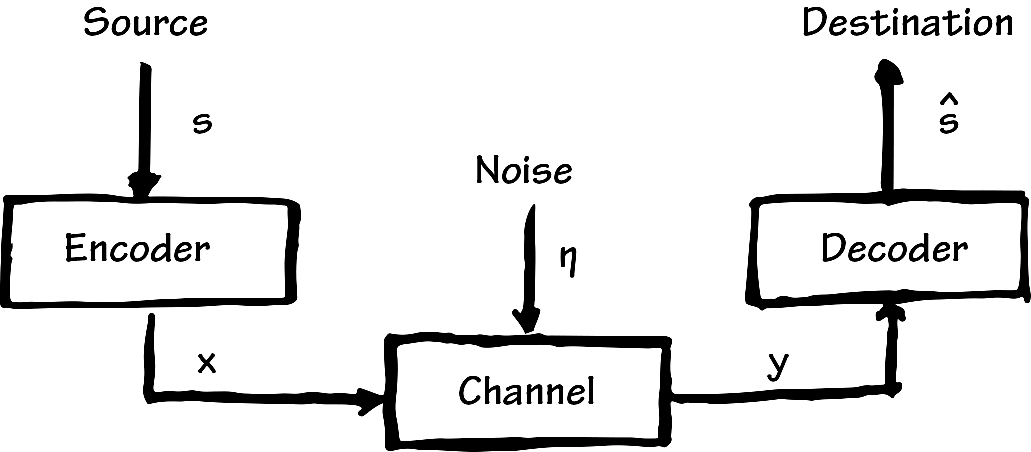
\includegraphics[width=\textwidth]{communication_setting}
	\caption{The communication problem setting.}\label{fig:communication_setting}
\end{figure}


The Source:
\begin{enumerate}
	\item selects a message  $\srcsymb$ from a set of possible messages $\srcalph$,
	\item encodes the message $\srcsymb$ into a string of symbols $\encsymb$, the signal,
	\item transmits this string of inputs $\encsymb$ through a noisy channel.
\end{enumerate}
\footnote{\(\srcalph\) is the alphabet or the set of possible outcomes of the random variable \(\src\).}

The Destination, then:
\begin{enumerate}
	\item receives a string of symbols \(\decsymb\),
	\item decodes the string \(\decsymb\) into the most probable message \(\hat{\srcsymb}\).
\end{enumerate}

\section{Information} The reason for communication is to change another agent's behaviour. In other words, \emph{communication either affects the conduct of the recipient, or it is like it has never happened}~\cite[p.100]{shannon:1948}. We have already established (\cref{sec:prob2info}, definition~\ref{def:information}) that \emph{information is what changes belief}; thus, changes an agent's conduct. So, \textbf{communication is transmitting information}.

Noteworthy, information is independent of the \emph{enconding} or the channel chosen. One can use any language (English, Portuguese, music, images, dance, etc.) and any means of transmission (letter, telegraphy, microwaves, etc.) that the transmitted information remains the same.

To simplify, Shannon constrained semantics to the act of choosing a message from a set of finite possibilities. A source (a person, a machine or phenomenon) that always sends the same message never surprises the receiver, and the message carries no information. On the contrary, a source that sends symbols at random is impossible to predict and, therefore, every message carries maximal information.

Therefore, in this setting, \emph{information is a measure of freedom of choice in selecting the message}~\cite[p.100]{shannon:1949}. In other words, it is a measure of surprisal or uncertainty reduction.

In the aforementioned famous paper, Shannon limited to say that mathematically, if the set of possible messages \(\srcalph\)  is finite, any function of the size of this set \(f(|\srcalph|)\) is a measure of information and that the logarithmic function is a natural choice. We shall expand on this idea.

\subsection{A guessing game}\label{guessing_game} Imagine a number from 1 to 1000. Let us assume that you picked the number at random. Thus, each number in the range had the same chance of being chosen, \(\frac{1}{1000}\). How many questions do I need to ask to guess your number correctly? Well, it depends on what are the allowed answers. I could ask:
\begin{wrapfigure}
	{L}{0.5
	\textwidth} \centering
	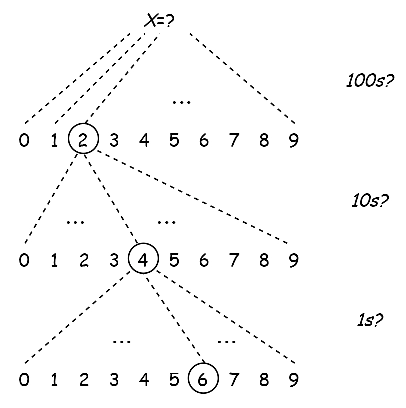
\includegraphics[width=0.45
	\textwidth]{246}
	\caption{Branching factor of 10 to find 246.}\label{fig:branching} \end{wrapfigure}
\begin{itemize}
	\item How many hundreds do your number have?
	\item Then, I would ask how many tens do your number have?
	\item Then, how many units?
\end{itemize}

In this case, the number of questions needed is three, the height of the tree in \cref{fig:branching}, because we allowed each answer to be a \emph{digit}; therefore, the \emph{branching factor} \(b\) of the decision tree was 10. It is easy to notice that the tree's height is \(\log_b (1000)\).

It is now clear what Shannon meant by saying that the logarithmic function was the natural measure of information. The logarithm will give the height (number of questions) of the decision tree based on the number of possible answers (the logarithm base). The branching factor is just a measurement unit and can be chosen arbitrarily.

The smallest branching factor is 2, a \emph{bit}. So, one bit is the amount of information that resulted from choosing between two equally likely options.

To solve the same guessing game with \emph{bits}, \ie with yes or no questions, one proceeds with a binary search, and in the worse case it will need \(\log_{2}(1000)=\frac{\log_{10}(1000)}{\log_{10}(2)}\approx 9.96 \therefore 10\) questions.

How about if the choice was among not equally likely options? Let us examine the simplest case of an unfair coin.

\Tree [.\(\rvX\)? [\(P(\rvX=H)=75\%\) \(P(\rvX=T)=25\%\) ] ]\\

Here, we expect the outcome to be \emph{heads}, so if it turns \emph{tails}, we get surprised. Before the coin flip, we were 25\% certain (our belief measure) that the \emph{experiment} would turn \emph{tails}. If it, in fact, turns \emph{tails}, our certainty reaches 100\%, growing by a factor of \(\frac{1}{0.25}=4\). So it is reasonable to think that our uncertainty of the \emph{tails} outcome decreased by a factor of 4 as well. We were 75\% certain that the \emph{experiment} would turn \emph{heads}. If it in fact turns \emph{heads}, our uncertainty of the \emph{heads} outcome decreased by a factor of \(\frac{1}{0.75}\approx 1.\overline{3}\). How do we transform this uncertainty reduction factor to a measure in bits? In other words, how do we measure in bits the information gained by unveiling an outcome?

Notice that 1 \emph{bit} is the amount of information that reduces uncertainty from 2 possible states to 1, a factor of 2. Also, 2 bits of information reduce the uncertainty from the 4 possible representable states with 2 bits to 1, a factor of 4.
\begin{align*}
	2^1 \text{ factor} &=  1\text{ bit} \\
	2^2 \text{ factor} &=  2\text{ bits} \\
	\cdots\\
	2^n \text{ factor} &= n\text{ bits}  \\
	\therefore x \text{ factor} &= \log_2 (x) \text{ bits}
\end{align*}
So, if an outcome has probability \(p(\encsymb)\):
\begin{align*}
	\frac{1}{p(\encsymb)} \text{ factor}  \implies \log_2 \frac{1}{p(\encsymb)} \text{bits} = - \log_2 p(\encsymb) \text{ bits}
\end{align*}

If the factor is a measure of the reduction in freedom of choice, the factor is the information gained by knowing the outcome of the \emph{experiment}. This factor is known as \textbf{self-information} or information content of an outcome\footnote{Information theory magnitudes are functions of the probabilities random variables and not directly of a random variable. To address this difference, we opt to use square brackets instead of parenthesis.}:
\begin{definition}\label{def:surprisal}
	The \textbf{information content, self-information, surprisal}, or \textbf{Shannon information} of a particular outcome \(\encsymb\) of an \emph{experiment} is defined as:
	\begin{align}
		I[\encsymb] = h[\encsymb]= -\log p(\encsymb)\\
		\tag{information content of outcome}
	\end{align}
\end{definition}
As we already had derived in \cref{sec:probability2information}.

\subsection{Entropy} In practice, however, we are not usually interested in the information of a particular outcome, but in how surprised, on average, we will expect to be with the entire set of possible outcomes.
\begin{definition}
	The entropy \(H[\rvX]\) of a random variable \(\enc\) is defined to be the average Shannon information content of its possible outcomes:
	\begin{align}
		H[\rvX] \eqdef \E_p \frac{1}{\log p(\encsymb)} = -\sum_{\encsymb \in \encalph} p(\encsymb) \log p(\encsymb) \text{ bits/symbol}.
	\label{eq:entropy} \end{align}
\end{definition}
\footnote{We will constrain our explanations of Information Theory to the discrete case. It can be argued that if we are interested in models that computers will use, some quantisation will always happen.}
Entropy can be seen in two ways:
\begin{enumerate}
	\item as the quantity of information ``produced'' by the source~\cite[p.18]{shannon:1949}.
	\item as a measure of \emph{uncertainty} or lack of pattern.
\end{enumerate}
Average information shares de same definition as Entropy; therefore, to know whether a quantity is information or Entropy depends on whether it is given or taken~\cite{stone:2015}. In other words, uncertainty reduced is information gained, and vice-versa. If a random variable \(\enc\) is very uncertain, then it has high Entropy. If we are told the outcome of the variable \(\rvX = \encsymb_j\), we have been given information that is equal to the uncertainty we had. Thus, receiving an amount of information is equivalent to having the same amount of Entropy taken away.

\section{The source} In the problem setting proposed by Shannon, the source generates a message, symbol by symbol. The choice of each symbol depends on the ``preceding choices as well as the particular symbols in question''~\cite[p.10]{shannon:1949}.

A mathematical model that follows this description is known as a \emph{stochastic process}. Any discrete source can be represented by a stochastic process. ``Conversely, any stochastic process may be considered a discrete source''~\cite{shannon:1949}.
\begin{definition}
	A \textbf{stochastic (or random) process} is a set of random variables indexed by a variable \(i \in \Natural\) (usually representing time):
	\begin{align}
		{\src_i}, i \in \Natural \\
		\tag{Stochastic Process}
	\end{align}
\end{definition}

In the original formulation, Shannon modeled the source as a stochastic process indexed by time. He thought the source as an entity that emits a certain rate, amount of information (bits) per period (seconds):
\begin{align}
\srcrate \eqdef \frac{H[\src]}{T_{\src}} \frac{\text{ bits}}{\text{ second}}
\end{align}
where \(T_{\src}\) is the average time in seconds of transmitting a symbol.
For simplification sake, from now on we will just say that the source rate is:
\begin{align}
	\srcrate = H[\src] \text{ bits/symbol}
	\end{align}
% We describe a stochastic process as \(\rvX_t = [\sA_{\rvX_t}, p_{\rvX_t}]\), where \(\sA_{\rvX_t}=\{\encsymb_t\}, t \in \sT\) is the alphabet from which the process chooses the symbols to emit; and \(p_{\rvX_t}=\{p_t\}, t \in \sT \) are the probabilities of choosing each symbol.

\subsection{Markov chains} More specifically, Shannon proposed using a special kind of stochastic process called an \emph{ergodic Markov chain} to model the source.
\begin{definition}
	An order-k \textbf{Markov chain} is a stochastic process that satisfies the following property:
	\begin{align}
		P(\src_i|\src_{i-1}, \src_{i-2}, \cdots, \src_{i-k})=P(\src_i|\src_{i-1}, \src_{i-2}, \cdots, \src_1)
	\end{align}
	The \textbf{ergodic} property means statistical homogeneity~\cite{shannon:1949}: its statistical properties can be deduced from a single, sufficiently long, random sample of the process.

\end{definition}
An order-k ergodic Markov chain is a process with a memory of \(k\) states. By modelling the source as an ergodic Markov chain, Shannon showed that his theory not only works for phenomena that can be modelled as i.i.d. random variables. The source can behave like a chain of random variables \( \{\src\}\), each representing an outcome \(\srcsymb \in \srcalph\) that are dependent on each other, as long as the sequence produced is longer than the number of symbols needed to the Markovian process achieve its stability.


\section{The encoder: Data compression}
\begin{quotation}
	\small \emph{ \flushright What’s in a name? \\
That which we call a rose,\\
by any other word would smell as sweet.\\
	\flushright --- Romeo and Juliet (act.2, sce.2), William Shakespeare\\
	\vspace{1cm} }
\end{quotation}
An encoding transforms information into data. The same information can be transformed into an audio file with spoken English, a piece of writing in Portuguese, or even an image. These encodings represent the information uniquely and differ in the amount of data (\emph{bits}) they use.

	\begin{figure}[hbt!]
		\centering
		\makebox[\largefigure][r]{
		\centering
		\begin{subfigure}
			[b]{.27\largefigure} \centering
			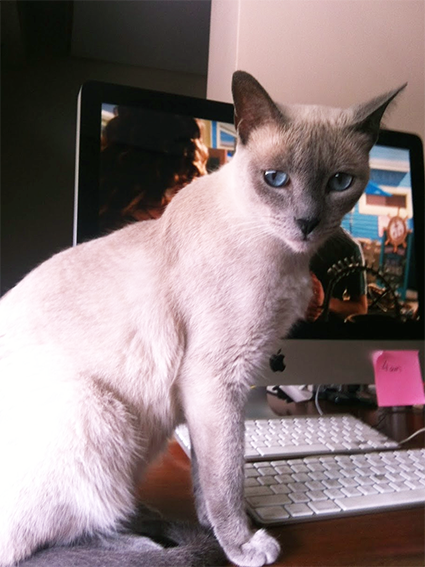
\includegraphics[width=
			\textwidth]{cutia-photo}
			\caption{360 Kb 15\small{cm}x20\small{cm} PNG colored image of a cat.}
		\end{subfigure}
		\hspace*{1em}
		\begin{subfigure}
			[b]{.27\largefigure} \centering
			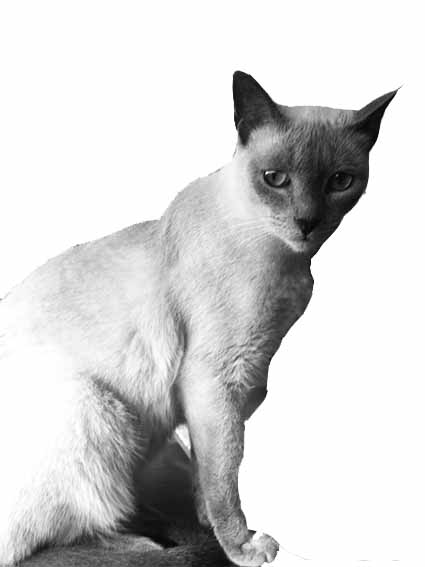
\includegraphics[width=
			\textwidth]{cutia-gray}
			\caption{  27 Kb 15\small{cm}x20\small{cm} JPG grayscale image of a cat.}
	\end{subfigure}
		\hspace*{1em}
		\begin{subfigure}
			[b]{.2733\largefigure} \centering
			
\includegraphics[width=
			\textwidth]{cutia-line}
			\caption{4.9 Kb 15\small{cm}x20\small{cm} SVG duotone image of a cat.}
	\end{subfigure}
	\hspace*{3.3cm}
}
\caption{Different representations of a cat and their encoding sizes in bits.}
\end{figure}




This idea may be better explained with an analogy with natural languages. Languages encode ideas into words in different ways~\cite{zaslavsky:2018}. For example, while in English's \emph{``to be''} is universal, Portuguese has two different verbs: \emph{``ser''} and \emph{``estar''}; the first for permanent, unchanging cases; the second for temporary situations such as mood or weather. At the same time, similar or identical
Meanings appear in unrelated languages~\cite{zaslavsky:2018}.

Thus, a message in a natural language can be translated (encoded) to another language and both messages will hardly have the same number of words, characteres, or size in \emph{bits}:
\begin{align}
	\srcblk=\{\src_1, \cdots, \src_n\}&~\underrightarrow{~encoding~}~
	\{\enc_1,  \cdots, \enc_k\}=\encblk.\\
\end{align}

Besides, some symbols are more important in a message: ``Mst nglsh spkrs wll ndrstnd ths phrs wtht vwls\footnote{``Most English speakers will understand this phrase without vowels''.}''. Here we created \emph{codewords} for words in English that a receiver can understand by the context (and certainly if she has a \emph{codebook}\footnote{A \emph{codebook} is a dictionary that relates words in the source alphabet, \(\srcalph\) to words, codes, in the encoder alphabet\(\encalph\).}).

Shannon's source coding theorem is about encoding messages efficiently, a form of data compression~\cite{stone:2015}. Here we present some definitions that will help us understand the theorem later.

\begin{definition}
A \textbf{(m, k) block code}, also known as a codebook, is a set of \(m\) codewords represented by a sequence of \(k\) bits:
\begin{align}
\{\enc^k(1),\enc^k(2),...,\enc^k(m)\},~\enc^k(i) \in \encalph^k, ~m \in \Natural.
\end{align}
\end{definition}
\begin{definition} The rate \(\sR_{\text{code}}\) of a (m,k) code is:
	\begin{align}
		\sR_{\text{code}} = \frac{\log m}{k}~\frac{\text{bits}}{\text{symbol}}\label{code_rate}
		\end{align}
\end{definition}
\begin{definition}
Let \(\srcblk\) be a block of \(n\) random variables, representing consecutive symbols \(\src_i \in \srcalph\) emited by the source. A \textbf{binary block encoder}  \(\enc\) is a function:
\begin{align}
	\enc:~ \srcalph^n \to {\{0,1\}}^k
\end{align}
that ``translates'' the block of source symbols (the message) into a code \(\encblk\) of \(k\) bits, using a \((|\srcalph^n|, k)\) code:
\begin{align}
	\enc(\srcblk)=\{\encsymb_1,  \cdots, \encsymb_k\}=\encvec \in {\{0,1\}}^k
\end{align}
\end{definition}
\begin{definition} The rate \(\encrate\) of a binary block encoder is:
	\begin{align}
		\encrate = \frac{\log |\srcalph^n|}{k}=\frac{n}{k}\log |\srcalph|~\frac{\text{bits}}{\text{symbol}}
		\end{align}
\end{definition}

% The efficiency of an encoder is its rate, how many useful bits it transforms per souce period (\(T_{\src}\)):
% \begin{align}
% 	n \text{symbols} = k \text{bits}\\
% 	\frac{n}{T_{\src}} \frac{\text{symbols}}{\text{seconds}}= \frac{k}{T_{\src}} \frac{\text{symbols}}{\text{seconds}}
% \end{align}

% The efficiency of the encoding \(\rvX^{k}\) can be defined by the rate:
% \begin{align}
% 	R_{\rvX} = \frac{k}{n} \frac{\text{bits}}{\text{symbol}}
% \end{align}
% Shannon's source coding theorem is essentially about data compression~\cite{stone:2015}.
% The encoding process yields inputs with a specific distribution \(p(\rvX)\). The shape of this distribution determines its entropy \(H[\rvX]\) and therefore how much information each input carries\cite{stone:2015}.

% We can interpret Shannon's source coding theorem in terms of data compression.  This interpretation was developed independently by Russian mathematician Andrey Kolmogorov(1933). He defined algorithmic complexity to be the length of the shortest computer program capable of describing a given object (e.g a message).  Algorithmic complexity is now known as Kolmogorov complexity\cite{stone:2015}.

% The encoding process yields a specific distribution \(p(\encsymb)\) to the channel input \enc. The distribution determines its entropy \(H[\rvX]\) and therefore how much information each symbol carries~\cite{stone:2015}.
% \begin{figure}[hbt!] \centering
% 	\includegraphics[width=
% 	.65\textwidth]{tubes3}
% 	\caption{Entropy of the source vs. coding capacity.}\label{fig:tube}
% \end{figure}
\begin{figure}[hbt!]
	\centering \makebox[
\largefigure][r]{
	\centering
	\begin{subfigure}
		[b]{.4\largefigure}
		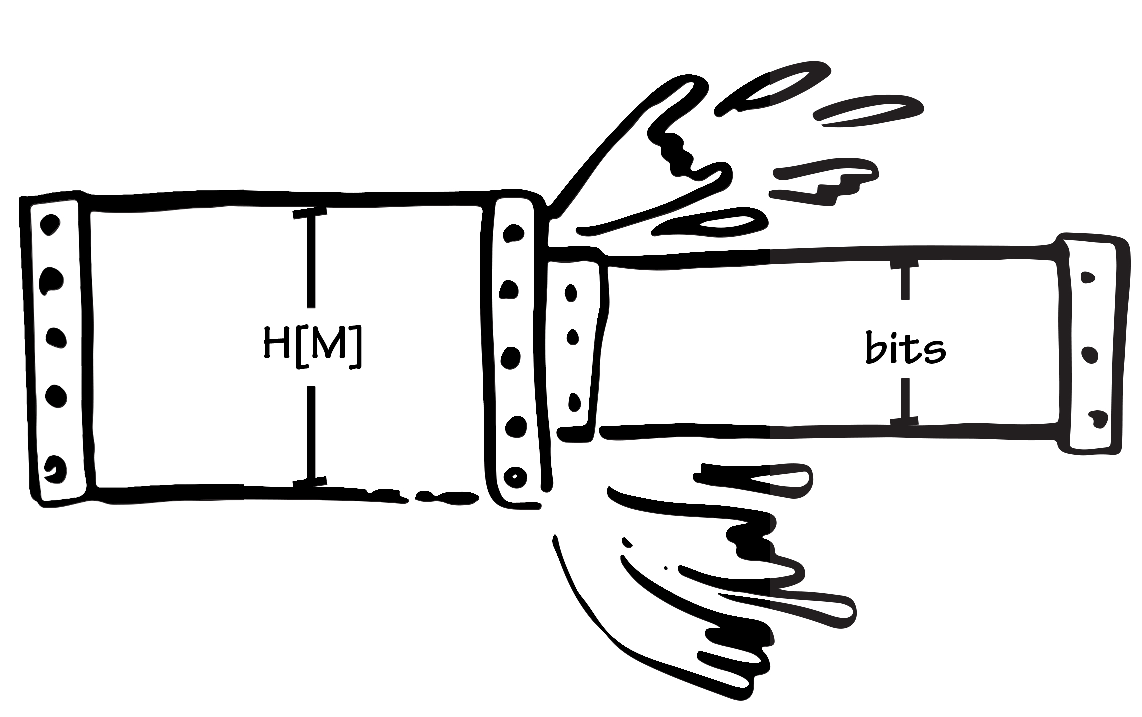
\includegraphics[width=
		\textwidth, left]{tubes5}
		\caption{Loss of information.}\label{fig:information_loss}
	\end{subfigure}
	\begin{subfigure}
		[b]{.4\largefigure} \centering
		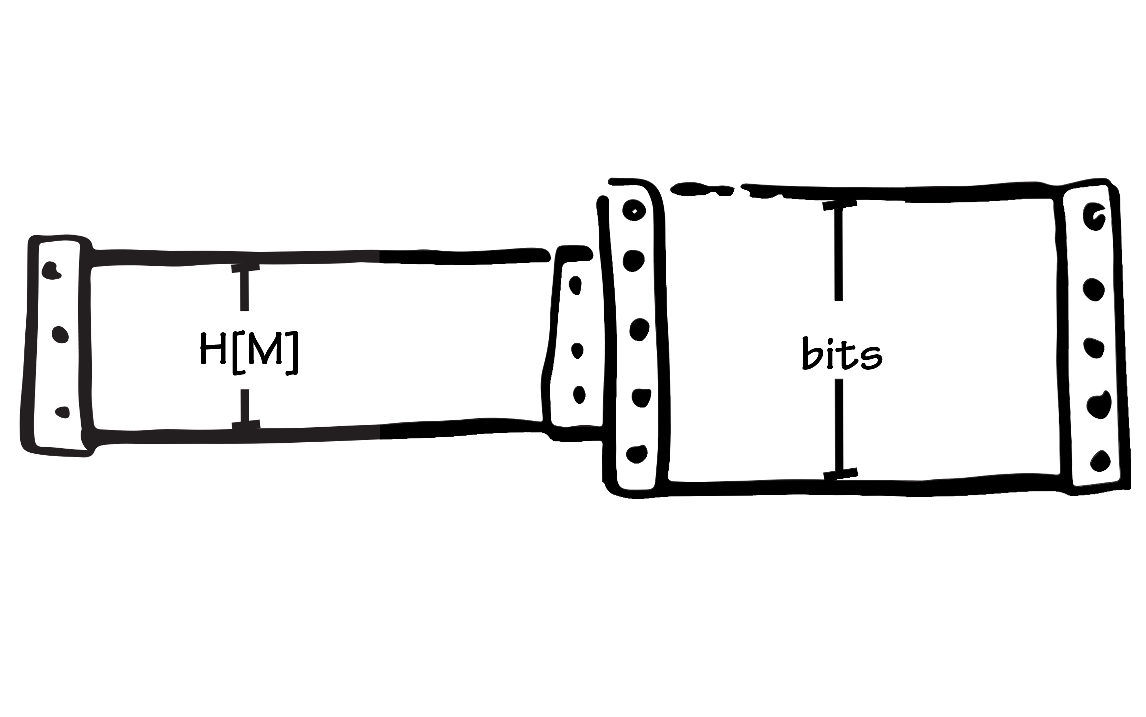
\includegraphics[width=
		\textwidth, left]{tubes6}
		\caption{ Waste of resources (bits).}\label{fig:resource_waste}
\end{subfigure}
\hfill
}
\caption{Entropy of the source vs. coding capacity.}\label{fig:tube}
\end{figure}
Shannon proved a relation between the source's entropy and its optimal encoding (this relation will be shown in \cref{sec:source_encoding_theorem}). The source's entropy is a lower bound on the minimum bits/symbol needed to encode it. The intuition is simple, imagine the Entropy of the source as a ``tube ``(see \cref{fig:tube}). The capacity of the tube is the rate of bits/symbol we expect from the source. The encoder is a connection to the tube.

If we use fewer bits than the entropy to encode it, we are losing information (see \cref{fig:information_loss}). If we use more bits than the entropy, we are wasting resources (see \cref{fig:resource_waste}).
\subsection{An encoding example}
Let us use an example to illustrate better this crucial concept in \ac{IT}\footnote{This example is inspired by~\citeauthor{geron:2018}}. Imagine you are building a weather station that sends the moment weather condition to a distant control room. Also, there are eight weather conditions in which we are interested. In this case, a message is the transmission of one symbol from \(\srcalph\).
\begin{align}
	\srcalph = \{\rw_0, \rw_1, \rw_2, \rw_3, \rw_4, \rw_5, \rw_6, \rw_7\}
\end{align}
\begin{figure}
	[hbt!] \centering
	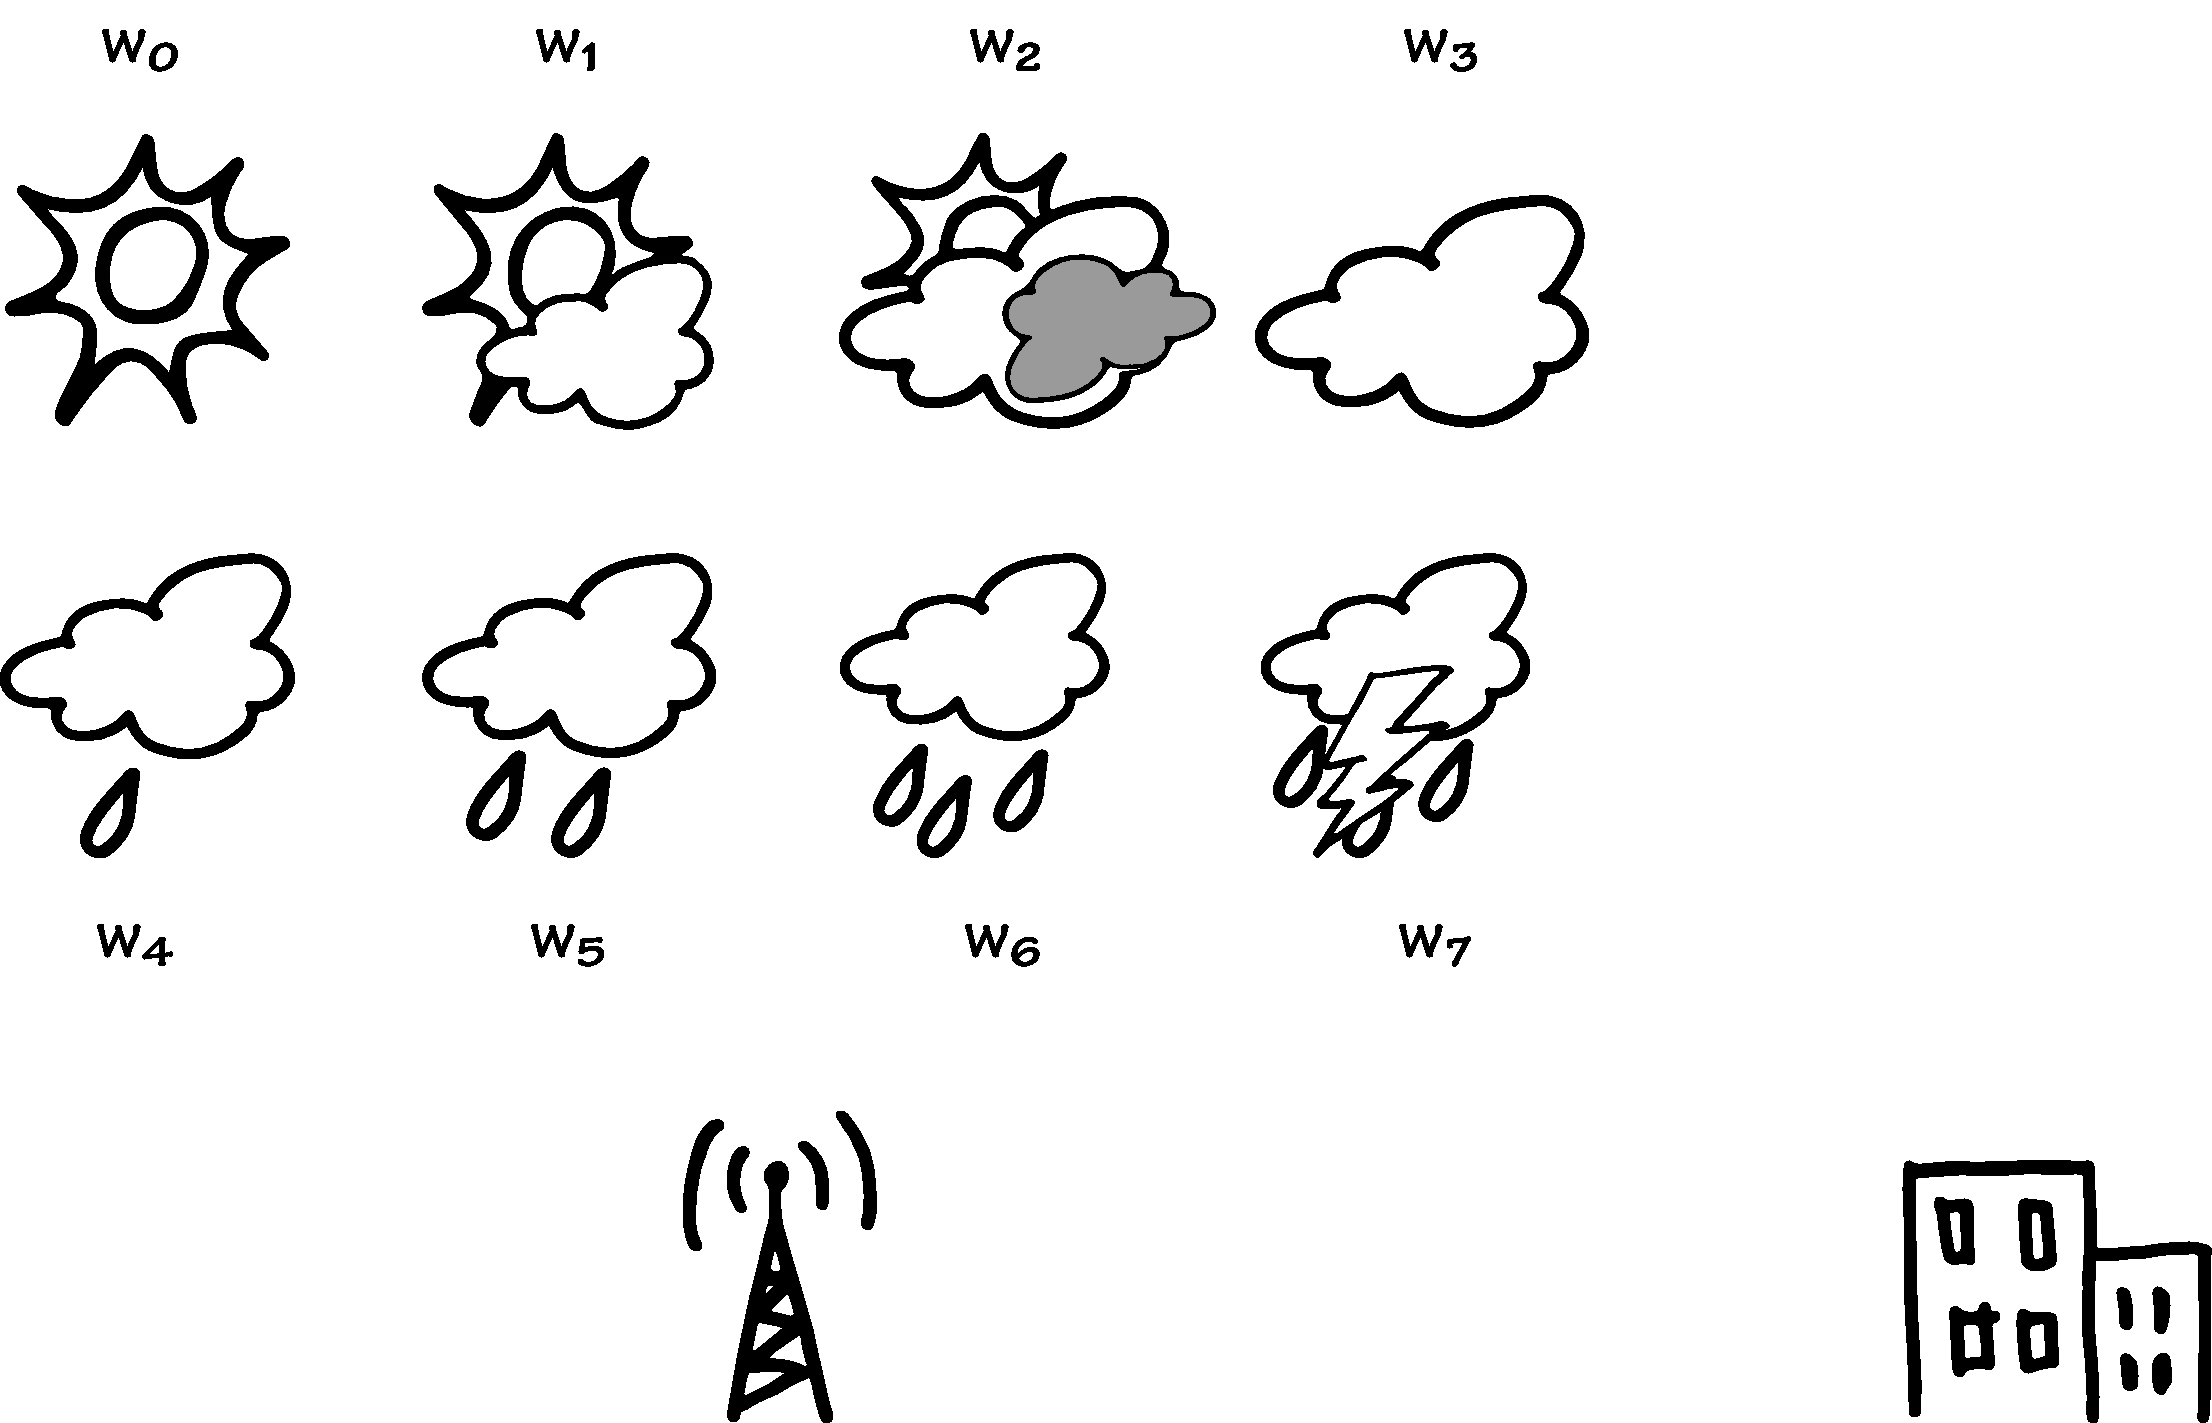
\includegraphics[width=
	\textwidth]{weather_station}
	\caption{A weather station.}\label{fig:weather_station} \end{figure}
How can we encode these weather conditions?

\subsection{Raw bit content} The first idea is to enumerate \(\srcalph\) in binary, using 3 bits/symbol.
\begin{align}
	\encalph = \{&\encsymb_0=000, \encsymb_1=001, \encsymb_2=010, \encsymb_3=011, \nonumber \\
	&\encsymb_4=100, \encsymb_5=101, \encsymb_6=110, \encsymb_7=111\} \label{example_encoding}
\end{align}
\begin{figure}
	[ht!] \centering
	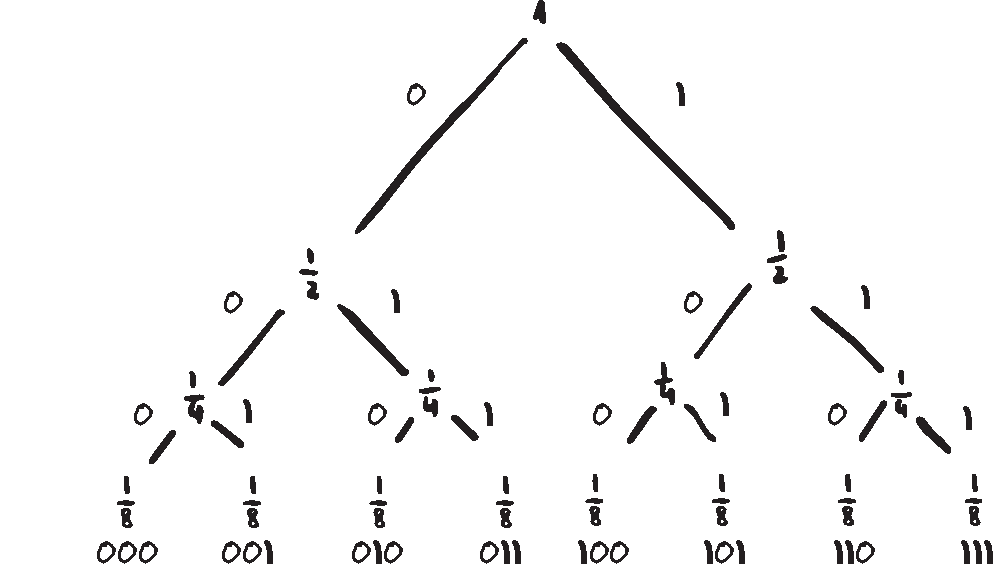
\includegraphics[width=
	\textwidth]{equi_tree}
	\caption{Largest encoding = Maximum entropy.}\label{fig:equi_tree} \end{figure}
This encoding provide a model of the source that has maximum entropy (all outcomes are equiprobable, thus have the same encoding size)\footnote{The probability distribution that produces maximum entropy is the \emph{uniform distribution} (\cref{sec:uniform_distribution})}:
\begin{align}
	p(\encsymb_i)&=\frac{1}{|\encalph|}, \forall i \in [0,7]\\
	H[\enc]&= - \sum^{|\encalph|}\frac{1}{|\encalph|} \log \frac{1}{|\encalph|}\\
	&= \log |\encalph|.
\end{align}
Is this a good encoding?

\subsection{Maximum Entropy Principle}
If all information we have is how many weather conditions are there, the size of the source alphabet, the best model is the one that conveys this information and has maximum Entropy, \ie{}it makes no further assumptions. This maximally entropic model have the worst-case scenario for the average number of questions needed to find out which outcome is the right one:
\begin{align}
	P({\src}) = \{&p_0=\tfrac{1}{8},p_1=\tfrac{1}{8},p_2=\tfrac{1}{8},p_3=\tfrac{1}{8}, \nonumber \\
	&p_4=\tfrac{1}{8},p_5=\tfrac{1}{8},p_6=\tfrac{1}{8},p_7=\tfrac{1}{8}\}
\end{align}

In this case, that encoding (\eqref{example_encoding}) is indeed a good option.
Notice that the encoding process yields a specific distribution \(P(\enc)\), which determines its entropy \(H[\enc]\) and, therefore, how much information per symbol it carries~\cite{stone:2015}. The maximum entropy is obtained with this equiprobable distribution, the \emph{uniform distribution} (\cref{sec:uniform_distribution}).

Let us assume now that another information about the source is given. The weather station is in Atacama, and \(P({\src'}) = \{p_0=75\%,p_1=10\%,p_2=5\%,p_3=1\%, p_4=1\%,p_5=1\%,p_6=1\%,p_7=1\% \}\).
\begin{figure}
	[ht!] \centering
	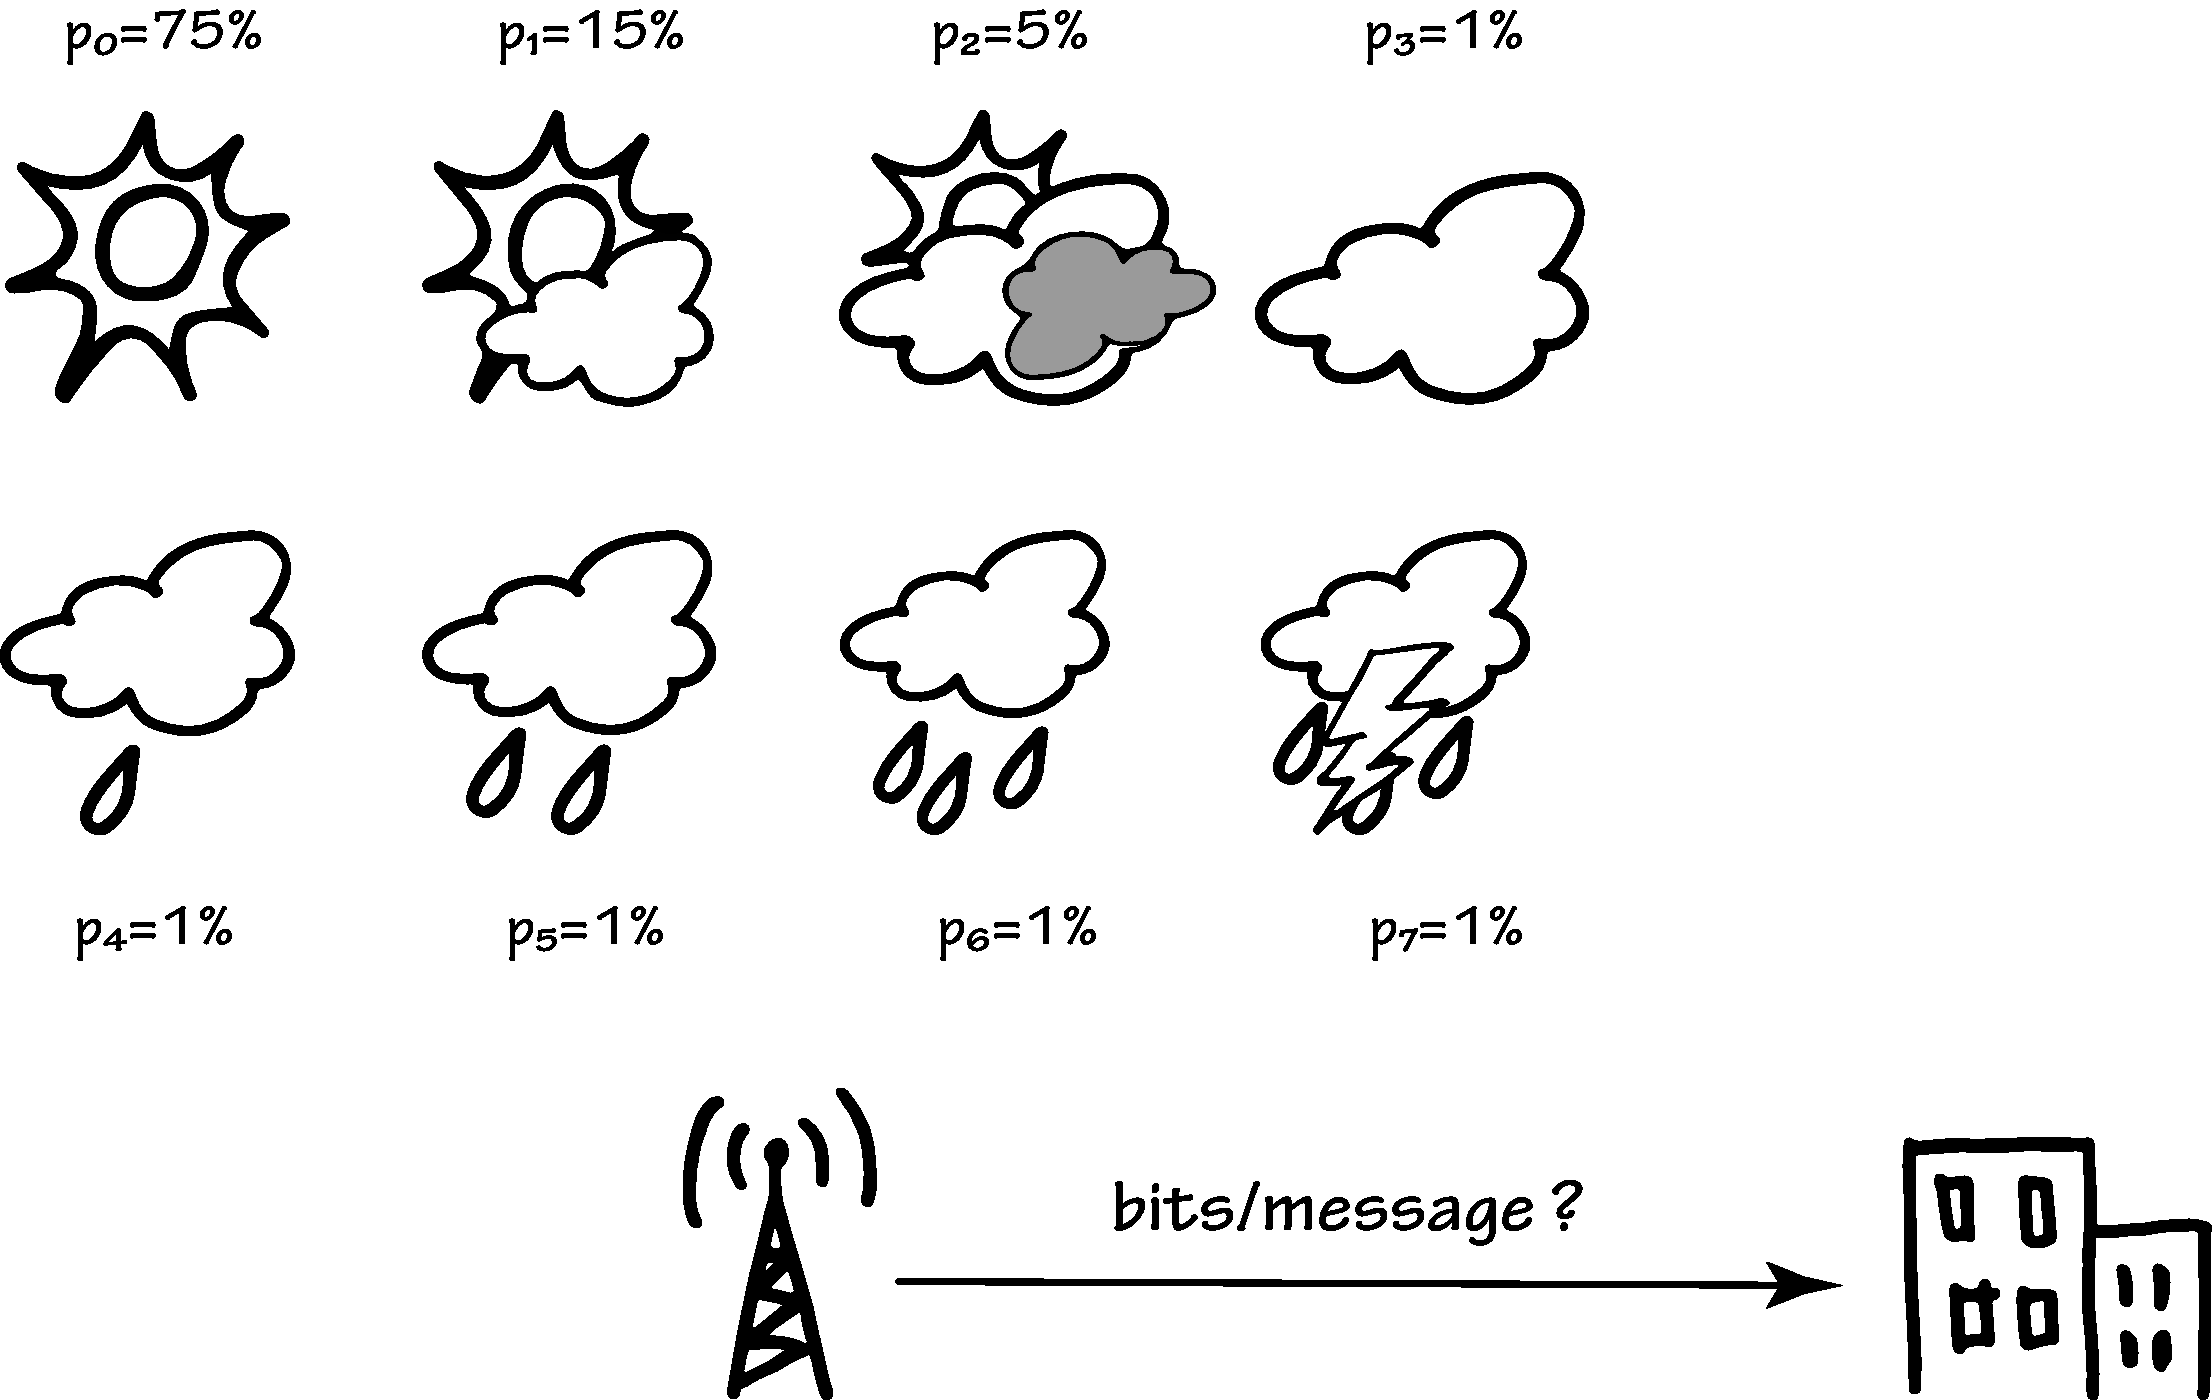
\includegraphics[width=
	\textwidth]{weather_station2}
	\caption{A weather station in Atacama.}\label{fig:atacama} \end{figure}
With this new information about the source. Can we do better? Sure.

First, let us calculate the lower bound (maximum efficiency) of the bits/symbol rate of the source encoding:
\begin{align}
	H[\src']&= 0.75 \log \frac{1}{0.75} + 0.15 \log \frac{1}{0.15} + 0.05 \log \frac{1}{0.05} + 5\biggl(0.01 \log \frac{1}{0.01}\biggr) \nonumber \\
	&\approx 1 \frac{\text{bits}}{\text{symbol}}
\end{align}

We know that theoretically we cannot have an encoding with less than 1 bit/symbol in average. But we can improve from 3 bits/symbol (see \cref{fig:inequi_tree})\footnote{Any distribution that is not uniform will lead to an average tree height that is smaller that the uniform distribution. The uniform distribution is the worst case.}:
\begin{figure}
	[hbt!] \centering
	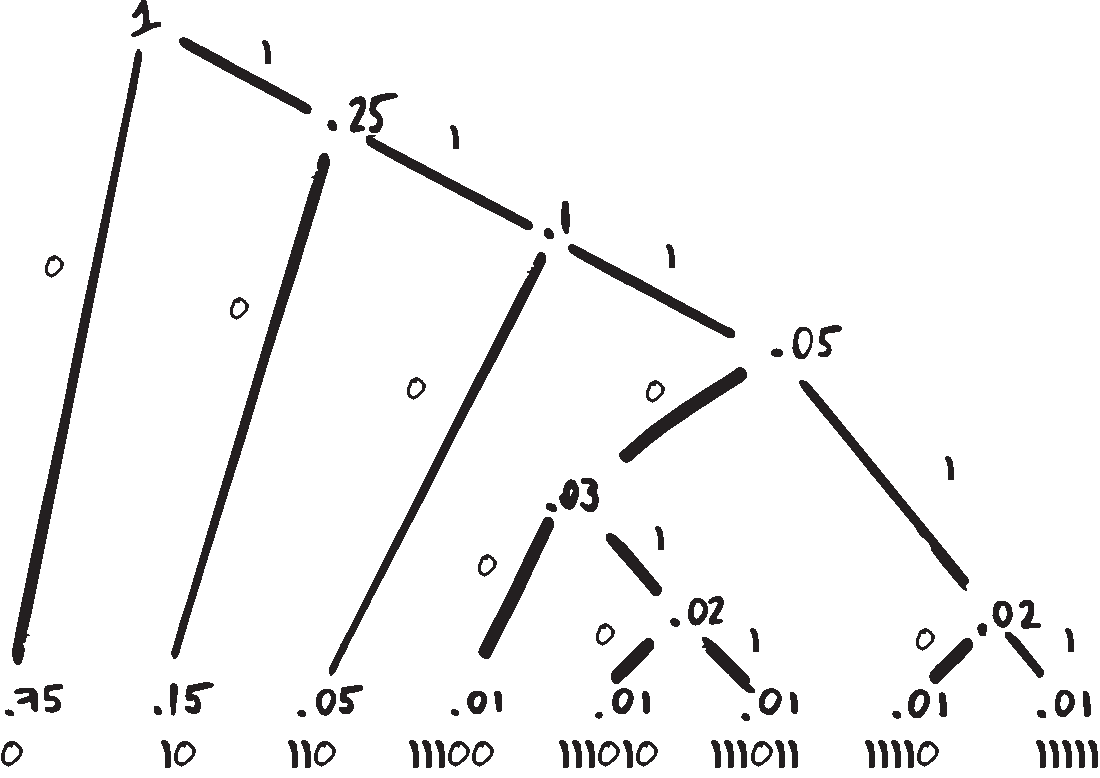
\includegraphics[width=
	.75\textwidth]{ineq_tree}
	\caption{The probability distribution of the source determines an encoding.}\label{fig:inequi_tree} \end{figure}
\begin{align}
	\sA_{\enc'} = \{&\encsymb'_0=0, \encsymb'_1=10, \encsymb'_2=110, \encsymb'_3=11100,\nonumber \\
	&\encsymb'_4=111010, \encsymb'_5=111011, \encsymb'_6=11110, \encsymb'_7=11111\}
\end{align}

The average encoding size per message symbol in \(\enc'\) is:
\begin{align}
	&0.75 \cdot 1 + 0.15 \cdot 2 + 0.05 \cdot 3 + 0.03 \cdot 5 + 0.02 \cdot 6 \nonumber \\
	&\approx 1.5 \frac{\text{ bits}}{\text{symbol}}
\end{align}

\subsection{Cross-Entropy}\label{sec:cross-entropy}
This average encoding size per message symbol has a special name: the Cross-Entropy. It is evident the similarity of the definition of Cross-Entropy and Entropy. If our model \(q\) of the real distribution \(p\) is absolute right, the Cross-Entropy is equal to the Entropy \(H_{p,q}=H_p\). If not (as it is in most cases), \(H_{p,q} > H_p \).

In our Atacama weather station example, the cross-entropy between the real distribution \(p=p(\srcsymb)\) and the encoding distribution \(q=p(\encsymb)\) was 1.5 bits/symbol. So, we can say the efficiency of the encoding \(\enc(\srcsymb)\) is \(\tfrac{\text{information}}{\text{data}} = \tfrac{H[\src]}{H_{p,q}[\src]} = \tfrac{1}{1.5} \approx 67\%\). We calculated  \(H_{p,q}\) knowing the sizes of each possible \(\srcsymb_i\).

Let us use another example, imagine that we transport the weather station from Atacama to London, where the probability distribution of the weather is \(P({\src''}) = \{p_0=5\%,p_1=5\%,p_2=10\%,p_3=15\%, p_4=15\%,p_5=20\%,p_6=20\%,p_7=10\% \} \therefore H[\src'']\approx 2.8\), and keep using the same encoding. It is obvious that the encoding will me much less efficient.
\begin{figure}
	[ht!] \centering
	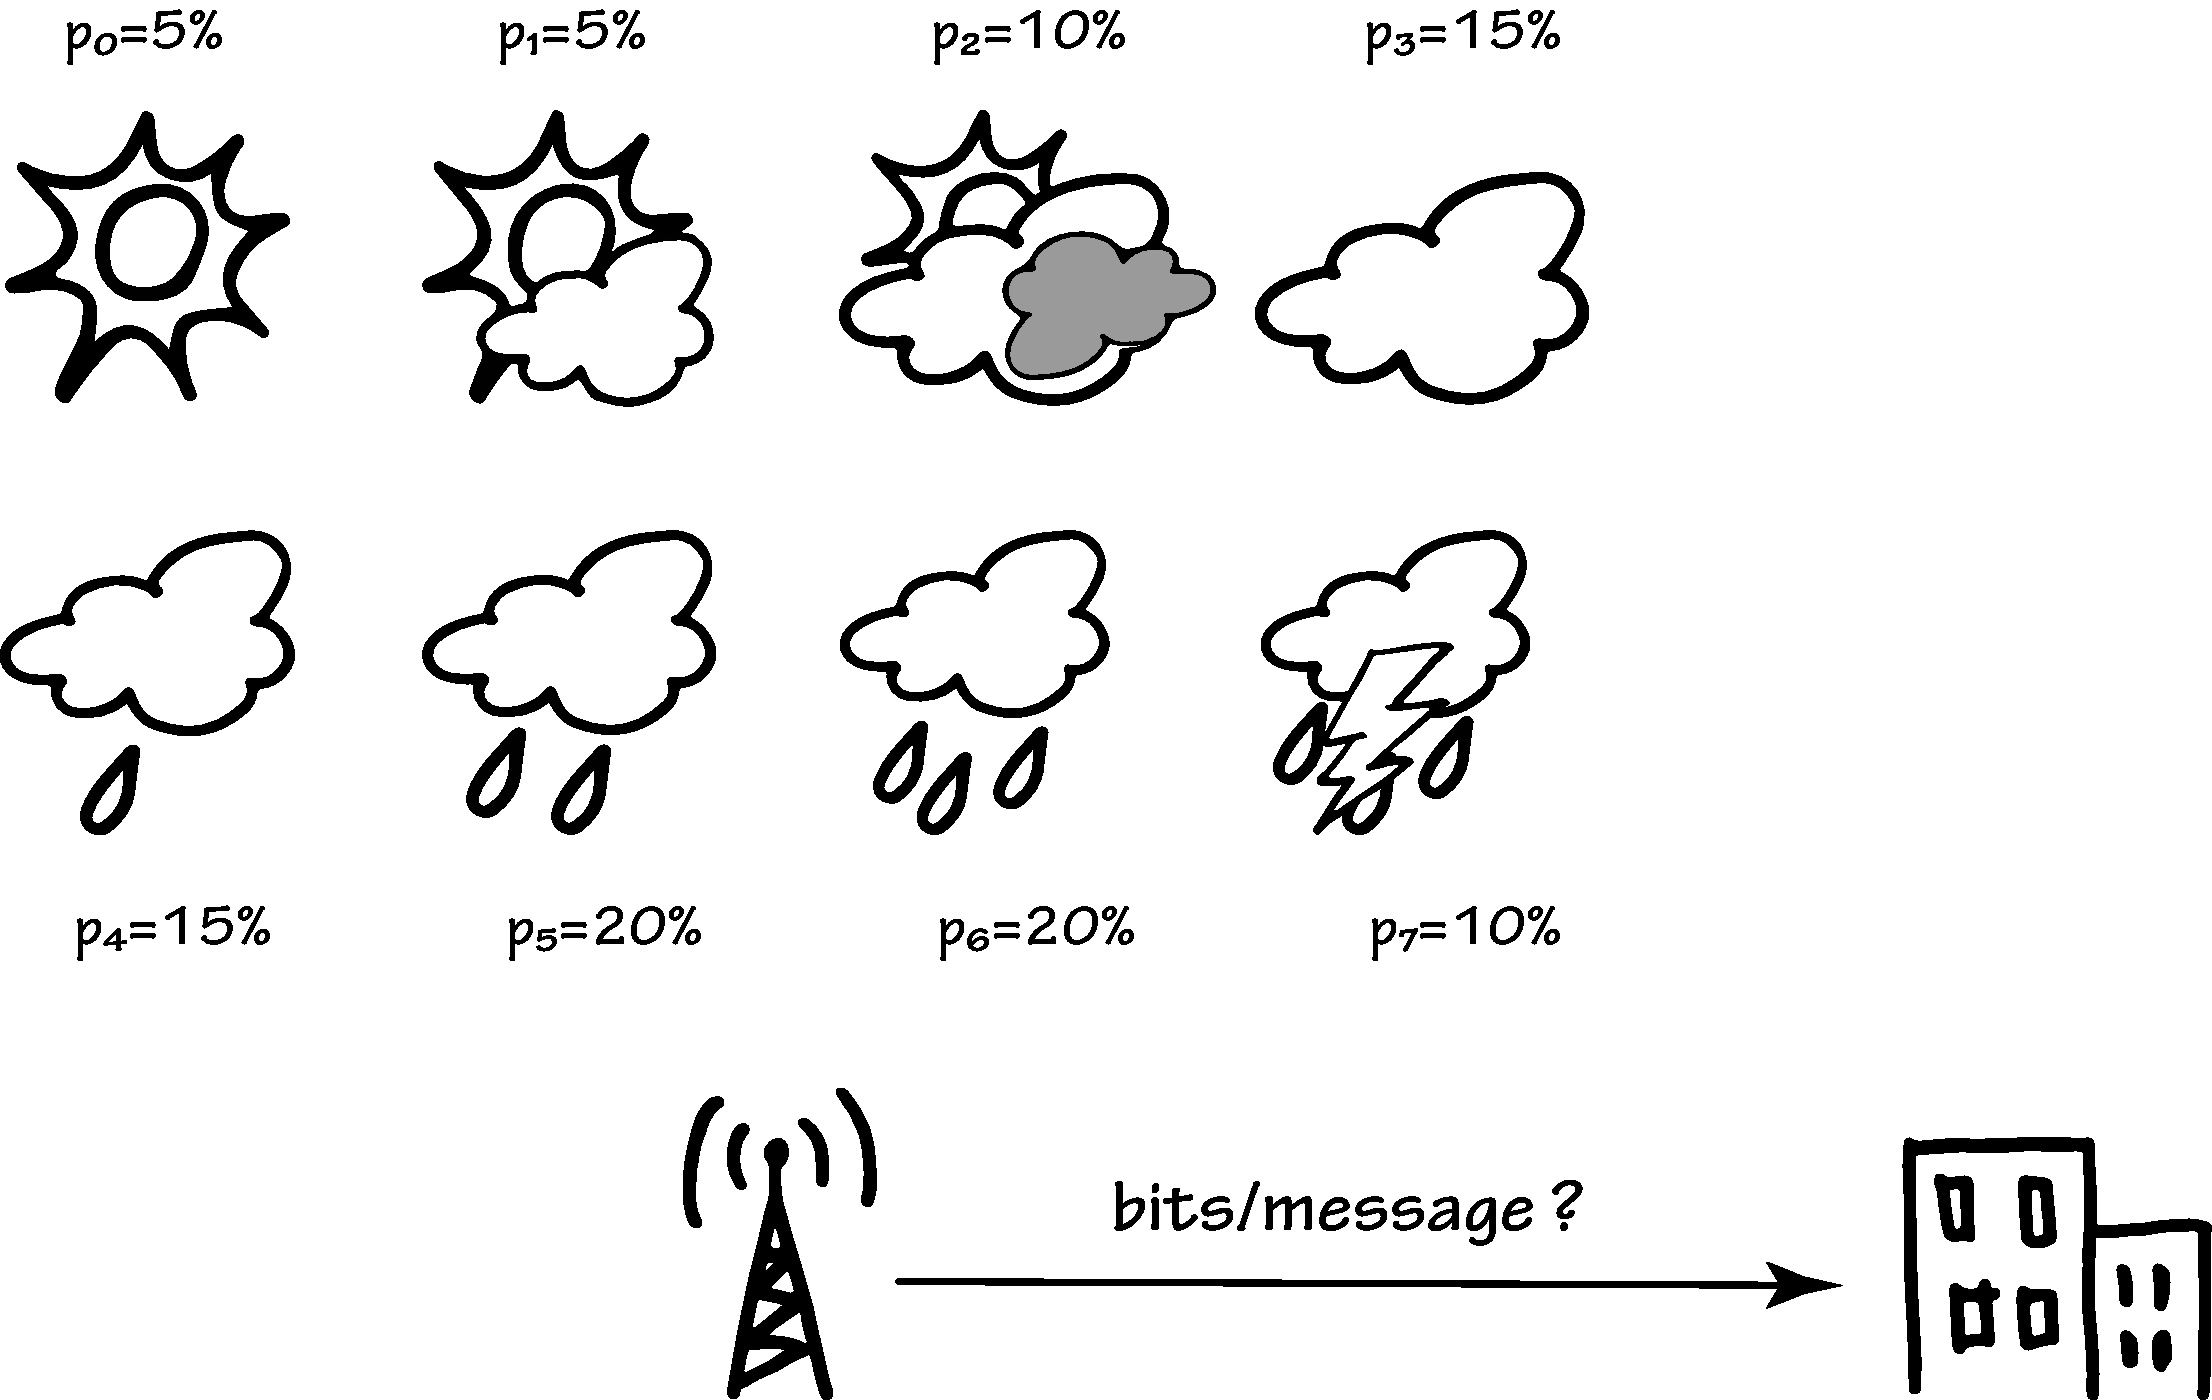
\includegraphics[width=
	\textwidth]{weather_station3}
	\caption{The Atacama's weather station in London.}\label{fig:london} \end{figure}
The average size of a message symbol in this situation is:
\begin{align}
	H_{p,q}[\src''],~ &p = P(\src''), q = P(\enc') \\
	&= 0.05 \cdot 1 + 0.05 \cdot 2 + 0.1 \cdot 3 + 0.45 \cdot 5 + 0.35 \cdot 6 \nonumber \\
	&\approx 4.8 \frac{\text{ bits}}{\text{symbol}}
\end{align}
\begin{definition}
	\textbf{Cross-entropy} is the average number of bits needed to encode data coming from a source \(\src\) with distribution \(p(\srcsymb)\) when using model \(q(\srcsymb)\).
	\begin{align}
		H_{p,q}[\src]=-\sum_{\srcsymb \in \sA_{\src}} p(\srcsymb) \log q(\srcsymb)
	\end{align}
\end{definition}

\subsection{KL Divergence (or Relative Entropy)} The amount by which the Cross-Entropy and the Entropy diverge is the KL Divergence:
\begin{definition}
	The \textbf{relative entropy or Kullback–Leibler divergence} between two probability distributions \(p(\srcsymb)\) and \(q(\srcsymb)\) that are defined over the same alphabet \(\srcalph \) is:
	\begin{align}
		\KL(p||q) = \sum_{\srcsymb} p(\src)~\log \frac{p(\srcsymb)}{q(\srcsymb)}\\
		\KL(p||q) = H_{p,q}[\src] - H_p[\src] \label{eq:KL_decomposition}
	\end{align}
\end{definition}
In our example:
\begin{align}
	\KL(p_{\text{Atacama}}||q_{\text{London}}) = \underbrace{H_{p,q}[\src'']}_{\approx 4.8} - \underbrace{H_p[\src'']}_{\approx 2.8} \approx 2 \frac{\text{bits}}{\text{symbol}}
\end{align}

\subsection{Shannon's source encoding theorem}\label{sec:source_encoding_theorem}
Now that we understand how the source encoding works, let us take a moment to appreciate the geniality of Shannon.  Here, we show how he demonstrated the size of the optimal encoding without ever explaining which encoding is that in the first place.

\begin{theorem}\label{th:source_encoding}
	The optimal binary enconding \(\enc^{k}=(X_1, \cdots, X_k),~ \enc_i \in \{0,1\}\),  of a n-symbols message \(\srcblk=(\src_1, \cdots, \src_n)\), where \(\src_i \in \srcalph\) are i.i.d.\footnote{An \st{obsessive} observant reader may have noticed that we are here considering the source as an i.i.d. stochastic process, instead of a stationay ergodic process.  This is the same proof stated by Shannon in~\cite{shannon:1948} and in several \ac{IT} books (\eg~\cite{cover:2006,mackay:2002}). A proof for ergodic finite alphabet sources can be found in~\cite{mcmillan:1953}.} \(\sim p(\srcsymb)\) has size \(k \approx n H[\src]\) for large \(n\).
\end{theorem}
\begin{proof}
	A one-to-one mapping \(\srcblk \mapsto \enc^{k}\) is invertible. If we enumerate all elements of \(\srcblk\) in binary, we will need \(k\) bits. Thus, with absolute certainty:
	\begin{align}
		k\leq \log \lceil|\srcblk |\rceil = \log \lceil 2^{n \log |\srcalph|}\rceil = n \log |\srcalph|+1~\text{ bits}\label{eq:k_upperbound}
	\end{align}
	Can we do better? We know from statistics that most possible outcomes are unlikely. In other words, there is a small set of very likely outcomes that is most probable. So let us use this property of Nature.
	\begin{figure}
		[ht!] \centering
		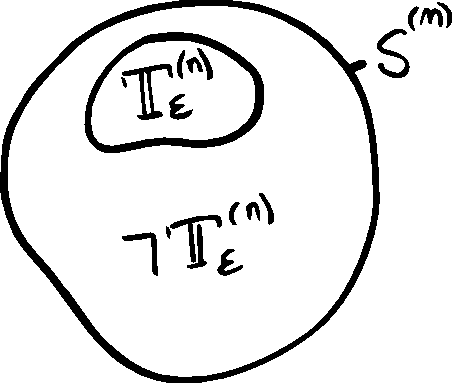
\includegraphics[width=.6\textwidth]{typicalset}
		\caption{The typical set of  sequences \(\srcblk\).}\label{fig:typical_atypical} \end{figure}

	We will divide all sequences \(\srcblk\) into two sets: the typical set (\(\typicalset\)) and its complement, the atypical set (\(\neg~ \typicalset\)), which can be seen in \cref{fig:typical_atypical}.

	\begin{definition}
		The \textbf{typical set} \(\typicalset\) with respect to \(p(\srcsymb)\) is the subset of sequences \(\srcblk=(\src_1,\cdots,\src_n ), \src_i \in \srcalph\), where:
		\begin{align}
			P(\typicalset)=\sum_{\srcblk \in \typicalset} P(\srcblk)> 1-\epsilon, \text{ for sufficiently large }n.\label{typical_set_definition}
		\end{align}
	\end{definition}
	In other words, for a sequence of \(n\) i.i.d random variables \(\src \equiv(\src_1,\cdots,\src_n )\), each drawn from \(p(\srcsymb)\), the outcome \(\vm=(\srcsymb_1, \cdots, \srcsymb_n)\) is almost certain to belong to the typical set \(\typicalset\), if n is large.

	Let us put aside that we do not know the size of the typical set, \(|\typicalset|\).

	We know that:
	\begin{align}
		|\typicalset| &\ll |\neg \typicalset| < |\srcblk |, \\
		P(\typicalset)&\gg P(\neg \typicalset ),\\
		\E(k) &= \lceil P(\typicalset)\log|\typicalset| + P(\neg \typicalset )\log |\neg \typicalset|\rceil.
	\end{align}

	Therefore, from~\eqref{eq:k_upperbound} we can predict that:
	\begin{align}
		\E(k) &\ll  n \log |\srcalph|+1~\text{ bits}
	\end{align}

	Now, we need to find \(|\typicalset|\). For this we will use the \acf{AEP}, formalized in the following Theorem~\cite{cover:2006}:
	\begin{theorem}[\ac{AEP}]\label{th:aep}
		If \(\src_1, \cdots, \src_n\) are i.i.d. from the same \(\sim p(\srcsymb)\), then:
		\begin{align}
			-\frac{1}{n}\log P(\src_1, \cdots, \src_n) \to H[\src] \text{ in probability.}
		\end{align}
	\end{theorem}
	\begin{proof}
		From the theorem definition,  \(\src_i\) are independent. Then from the Product Rule (eq. \ref{eq:Product_Rule}):
		\begin{align}
			- \frac{1}{n} \sum_{i=1}^{n}P(\underbrace{\src_1, \cdots, \src_n}_{\srcblk}) &\overset{\text{~eq.\ref{eq:Product_Rule}}}{=} -\frac{1}{n} \log(\prod_{i=1}^{n} \cancelto{p(\srcsymb)}{P(\src_i))}\\
			&=\frac{1}{n} \sum_{i=1}^{n} -\log p(\srcsymb)
		\end{align}
		From the weak law of large numbers:
		\begin{align}
		 n \to \infty,~\frac{1}{n} \sum_{i=1}^{n}\xi_i \to \mathbb{E}(\xi) \label{eq:law_large_numbers}
		\end{align}
		Therefore, using the fact that a statistic of a random variable is a random variable, let \(\xi=- \log P(\src_i)\)~\cite{cover:2006} and using~\eqref{eq:entropy} and~\eqref{eq:law_large_numbers}:
		\begin{align}
			n \to \infty,& \nonumber\\
			\frac{1}{n} \sum_{i=1}^{n}(- \log P(\src_i))
			&\to \underbrace{\E_p (- \log p(\srcsymb))}_{H[\src]}\\
			\therefore -\frac{1}{n}\log P(\srcblk) &\to H[\src]~\qed
		\end{align}
	\end{proof}
		Now that we proved the \ac{AEP} theorem (Theorem~\ref{th:aep}), let us use it to define \(|\typicalset|\):
		\begin{align}
			-\frac{1}{n} \log P (&\srcblk)\to H[\src] \text{ in probability}\\
			P (&\srcblk) \to 2 ^{-n(H[\src])} \therefore\\
			2 ^{-n(H[\src] + \epsilon)}\leq P (&\srcblk)\leq 2 ^{-n(H[\src] - \epsilon)} \text{ in probability}\label{eq:epsilon}
		\end{align}
		We also now that:
		\begin{align}
			1 &= \sum_{\srcblk} P(\srcblk)\\
			1 &\geq \sum_{\srcblk \in \typicalset}P(\srcblk)\\
			1 &\geq |\typicalset|~ P(\srcblk)
		\end{align}
		From~\eqref{eq:epsilon}:
		\begin{align}
			1 &\geq |\typicalset|~ 2 ^{-n(H[\src] + \epsilon)}\\
			\therefore~ |\typicalset| &\leq 2 ^{n(H[\src] + \epsilon)}\label{eq:typical_upperbound}
		\end{align}
		This upper bound to \(|\typicalset|\) is all we need to prove source coding theorem (Theorem~\ref{th:source_encoding}).
		\begin{align}
			\E(k) &= \lceil P(\typicalset)\log|\typicalset|  \nonumber \\
			&+ \cancelto{\epsilon}{P(\neg \typicalset)} \cancelto{|\srcblk|=n \log |\srcalph|}{\log |\neg \typicalset|} \rceil \\
			&\simeq \lceil (1-\epsilon)\log 2^{n(H[\src]+\epsilon)} + \cancelto{\epsilon' n}{\epsilon n \log |\srcalph|}\rceil\\
			&\simeq \lceil (1-\epsilon)[n(H[\src]+\epsilon)] + \epsilon' n \rceil\\
			&\simeq \lceil n(H[\src]+\epsilon - \epsilon n H[\src] - \epsilon^2) + n (\epsilon')\rceil\\
			&\simeq \lceil n(H[\src]+\cancelto{\epsilon''}{\epsilon - \epsilon H[\src] - \epsilon^2}) +  n (\epsilon')\rceil\\
			&\simeq \lceil n(H[\src]+\epsilon''+\epsilon')\rceil = \lceil n(H[\src]+\varepsilon)\rceil\\
			\therefore \nonumber\\
			\E(k) &\simeq n H[\src] \qedhere
		\end{align}
	\end{proof}
	We proved that the average information per symbol of the coding generated by the optimum encoder has the same average information per symbol as the source, \(H[\src]\frac{\text{bits}}{\text{symbol}}\). Due to this property, it is quite common to talk about \(H[X]\) as the entropy of the source.
\subsection{Typical Set}
In the proof of the source coding theorem, we defined the typical set and discovered some of its properties, but we left one behind. We only needed the upperbound of the \(|\typicalset|\), let us now derive its lowerbound.
From~\eqref{eq:epsilon} and the typical set definition (\eqref{typical_set_definition}):
	\begin{align}
		\sum_{\srcblk \in \typicalset}2^{-n(H[\src]-\epsilon)}&\geq 1 - \epsilon\\
		|\typicalset|2^{-n(H[\src]-\epsilon)}&\geq 1 - \epsilon\\
		|\typicalset|&\geq (1 - \epsilon)2^{n(H[\src]-\epsilon)}\label{eq:typical_lowerbound}
	\end{align}
	Therefore, from~\eqref{eq:typical_lowerbound} and~\eqref{eq:typical_upperbound} we can derive:
\begin{align}
	 (1 - \epsilon)2^{n(H[\src]-\epsilon)} \leq &|\typicalset| \leq 2 ^{n(H[\src]+\epsilon)}\\
	 &|\typicalset| \to 2 ^{nH[\src]}\label{eq:typical_set_size}
\end{align}
With that, we can list some useful properties of \(\typicalset\):
	\begin{enumerate}
		% [i.]
		\item almost all probability is concentrated in the typical set, by definition (\eqref{typical_set_definition});
		\item elements in the typical set are nearly equiprobable,~\eqref{eq:epsilon};
		\item the number of elements in the typical set is nearly \(2^{H[\src]}\),~\eqref{eq:typical_set_size}.
	\end{enumerate}
Going back to the \ac{AEP} theorem (Theorem~\ref{th:aep}):
\begin{align}
	&\frac{1}{n}\log \biggl(\frac{1}{P(\srcblk)}\biggr) &\to H[\src] \nonumber\\
	H[\src] -\epsilon \leq 	&\frac{1}{n}\log \biggl(\frac{1}{P(\srcblk)}\biggr)\leq H[\src] +\epsilon
\end{align}

We can think of the middle term as the Entropy of a sample of size \(n\). Thus a typical sample gives us an amount of information close to the average information from the source, \(H[\src]\)\footnote{This insight reminds us of the sample complexity, which will be discussed in \cref{ch:mlt}}.

\section{The channel: Data transmission} The channel is simply the medium used to transmit the signal \(\encvec\) from the encoder to the decoder. It may be anything from a band of radio frequencies, an electrical wire, a beam of light, or a postal service. As we did before, we can also think the channel as a ``tube'' which carries information (see \cref{fig:tube})\footnote{This definition of a discrete channel covers the deterministic case where \(\decsymb = f(\encsymb)\).\\ In most cases, the usage of a channel is determined by the period in which it is being used.  Thus, some prefer to define the capacity in bits/second.}.

\begin{definition}
	Mathematically, a \textbf{discrete channel} is the conditional probability
	\begin{align}
		p(\decsymb|\encsymb), \decsymb \in \decalph, \encsymb \in \encalph.
	\end{align}
\end{definition}
\subsection{Noiseless Channel Capacity}
\begin{definition}
	The \textbf{operational capacity} of a channel is the maximum rate of bits per usage that the medium is physically capable of transmitting. It is in fact just a number of bits per usage. We can think of it as the maximum entropy it is capable of transmiting in the absence of noise:
	\begin{align}
		\sC_{\text{operational}}= R = \max_{p(\encsymb)} \log |\encalph| \text{ bits/usage}.
	\end{align}
	% In other words, the \emph{operational capacity} \(\sC\) is achieved by the distribution \(p(\encsymb)\) which makes \(H[\enc]\) as large as possible.
\end{definition}

\subsection{The noisy channel}
\begin{figure}
	[hbt!] \centering
	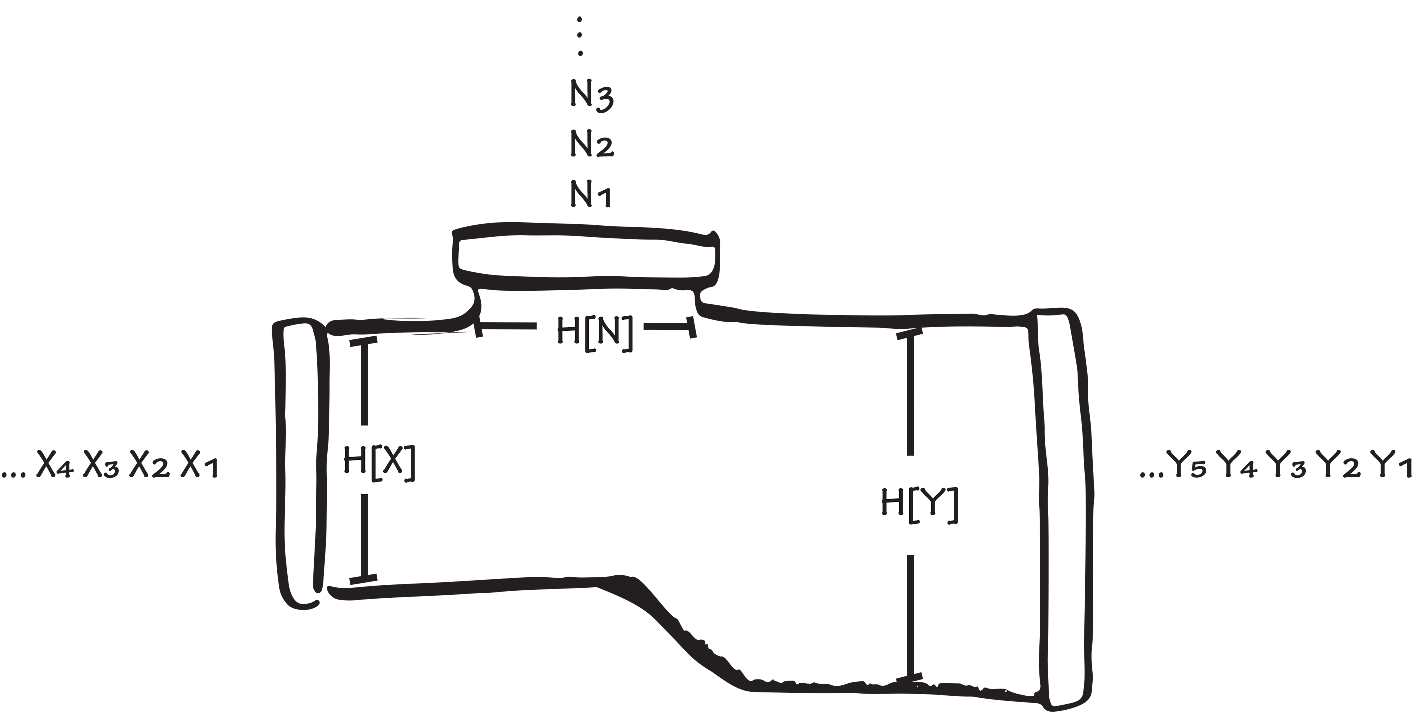
\includegraphics[width=
	\textwidth]{channel}
	\caption{The noisy channel.}
\end{figure}
 All practical communications, however, are noisy~\cite{stone:2015}. Noise reduces the rate at which information can be communicated reliably. Shannon proved that information could be communicated, with arbitrarily small error, at a rate limited only by the channel capacity.

 To understand how noise affects the channel capacity, we need to understand the concepts of \textbf{conditional entropy}, \textbf{joint entropy} and \textbf{mutual information}.
\subsection{Conditional Entropy} The residual uncertainty we have about a random variable \(\dec\), given that we already know the outcome of another random variable \(\enc\) is the \textbf{conditional entropy}:
\begin{definition}
	The \textbf{conditional entropy} or \textbf{equivocation} \(H[\enc|\dec]\) of \(\enc\) given \(\dec\) is:
	\begin{align}
		H[\enc|\dec] &\eqdef \sum_{\decsymb \in \decalph} p(\decsymb) \left[ \sum_{\encsymb \in \encalph} p(\encsymb|\decsymb) \log \frac{1}{p(\encsymb|\decsymb)}\right]\\
		&=- \sum_{\encsymb\decsymb \in \encalph\decalph} p(\encsymb,\decsymb) \log p(\encsymb|\decsymb)
	\end{align}
\end{definition}
% \paragraph{chain rule} From the Product Rule of probabilities (\eqref{eq:Product_Rule}), we have:
% \begin{align}
% 	\log \frac{1}{p(x,y)} = \log \frac{1}{p(x)+ \log \frac{1}{p(y)}}\\
% 	\therefore H[\enc,\dec]=H[\enc]+H[\dec|\enc]
% \end{align}
\subsection{Joint Entropy}
We have defined the entropy of a single random variable in~\eqref{eq:entropy}. Now, we extend the definition to a pair of random variables. As the pair can be seen as a single vector-valued random variable, there is nothing new in this definition~\cite[p.15]{cover:2006}.
\begin{definition}
	The \textbf{joint entropy} \(H[\rvX, \rvY]\) of a pair of discrete random variables \((\rvX, \rvY)\) with joint distribution \(p (x, y)\) is defined as:
	\begin{align}
		H [X,Y] &\triangleq -\E \log P(\rvX, \rvY) \\
		&= - \sum_{\encsymb \in \sA_x} \sum_{\decsymb \in \sA_y} p(\encsymb,\decsymb) \log p(\encsymb,\decsymb).
	\label{eq:joint_entropy} \end{align}
\end{definition}
\subsection{Mutual Information}
\begin{definition}\label{def_mutual_information}
	The \textbf{mutual information} \(I[\enc;\dec]\) between two variables, such as a channel input \(\enc\) and output \(\dec\), is the amount of information obtained about one random variable through observing the other random variable.
	\begin{align}
		I[\enc;\dec] &= \sum_i \sum_j p(\encsymb_i, \decsymb_j) \log \frac{p(\encsymb_i, \decsymb_j)}{p(\encsymb_i) p(\decsymb_j)} \text{ bits} \label{eq:mutual_information}\\
		&= H[\enc] - H[\enc|\dec]\\
		&= H[\dec] - H[\dec|\enc]\\
		&= H[\enc] + H[\dec] - H[\enc, \dec]\\
		&= H[\enc, \dec] - [H[\enc|\dec] + H[\dec|\enc]] \text{ bits}
	\end{align}
\end{definition}
\begin{figure}
	[hbt!] \centering
	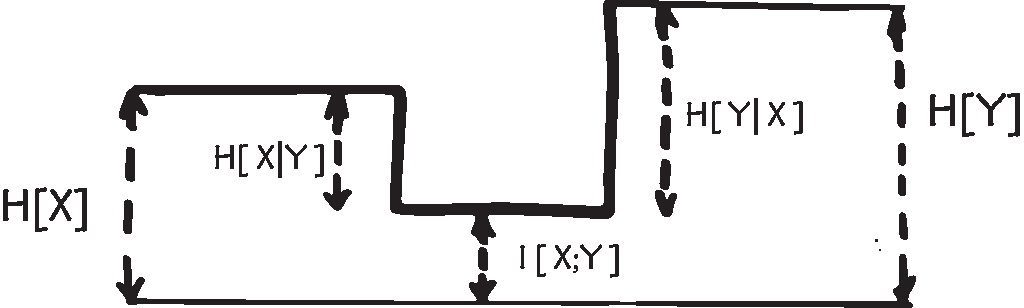
\includegraphics[width=\textwidth]{mutual}
	\caption{Relationship between information measures in a channel.}\label{fig:mutual}
\end{figure}
For a visual understanding of this measures, see \cref{fig:mutual}.
The mutual information can also be seen as a measure of the mutual dependence between the two variables, as the mutual information is the same as the Kullback–Leibler divergence between the joint distribution and the product of the variables marginal distributions:
\begin{align}
	I[\enc;\dec] = \KL(p(\encsymb, \decsymb)||p(\encsymb)p(\decsymb)) .
\end{align}

\subsection{Data Processing Inequality}
We cannot increase information by applying a deterministic function to the data, nor decrease information if the deterministic function is invertible.

\begin{theorem}
	[DPI\footnote{We refer to~\cite[th.2.8.1]{cover:2006} for a proof}] Let three random variables form the Markov chain \(\rvX \rightarrow \rvY \rightarrow \rvZ\), implying:
	\begin{align}
		p(\rx,\ry,\rz)=p(\rx)p(\ry|\rx)p(\rz|\ry).
	\end{align}
	No processing of \(\rvY\), deterministic or random, can increase the information that \(\rvY\) contains about $\enc$:
	\begin{align}
		I[\rvX;\rvY] \geqslant I[\rvX;\rvZ]
	\end{align}
\end{theorem}
\begin{theorem}
	[Reparemetrisation invariance] $I[\rvX;\rvY]\geqslant I[\rvX;g(\rvY)]$: functions of the data $\rvY$ cannot increase the information about $\rvX$.\label{th:reparemetrisation_invariance}
\end{theorem}
\begin{proof}
	\(\rvX \rightarrow \rvY \rightarrow \rvZ\) form a Markov Chain	where $\rvZ=g(\rvY) \therefore I[\rvX;g(\rvY)]=I[\rvX;\rvZ]$. By DPI:\@
	\begin{align}
		I[\rvX;\rvY] \geqslant I[\rvX;\rvZ]\\
		I[\rvX;\rvY] \geqslant I[\rvX;g(\rvY)]
	\end{align}
\end{proof}



\subsection{Noisy channel capacity}
Given that in a noise channel \(\dec = \enc + \noise \), where \(\noise\) is the noise in the channel, from the mutual information definition:
\begin{align}
	I[\enc;\dec]&=H[\dec] - H[\dec|\enc]\\
	&=H[\dec] - H[(\enc + \noise)|\enc].
\end{align}
If $\enc$ is known, the uncertainty from $\enc$ is none:
\begin{align}
	I[\enc;\dec]&=H[\dec] - H[\noise|\enc]
\end{align}
By definition, $\noise$ and $\enc$ are independent, therefore:
\begin{align}
	I[\enc;\dec]&=H[\dec] - H[\noise]\\
	\therefore H[\dec|\enc] &= H[\noise]
\end{align}
% The kind of channel that we are interested in is called an addictive channel, where:
% \begin{align}
% 	\dec &= \enc + \eta \\
% 	H[\dec]&= I[\enc;\dec] + H[\eta]\\
% 	&= I[\enc;\dec] + H[\dec|\enc]
% \end{align}

\begin{definition}
	The \textbf{information capacity} or \emph{effective capacity} of a noisy channel is defined as:
	\begin{align}
		C &= \max_{p(x)} I[\enc,\dec]\\
		&=\max_{p(x)} (H[\dec] - H[\dec|\enc]) \text{ bits/usage.}\\
		&=\max_{p(x)} (H[\enc] - H[\enc|\dec]) \text{ bits/usage}.
	\end{align}
\end{definition}
The information capacity can be derived theorem from Shannon's noisy channel theorem (\ref{noisy_channel_theorem}). Notice that when there is no noise, the definition corresponds to the \emph{operational capacity} definition.

% There is a duality between compression and transmission~\cite{cover:2006}. In compression we remove redundancy to obtain the smallest representation of the message, whereas in transmission we add redundancy in a controlled fashion in order to be able to recover from errors caused by noise in the channel.
\section{The decoder}
The decoder capability of reconstructing the message from the encoded data despite the channel noise is a direct consequence of Shannon's second theorem:

\subsection{Shannon's noisy channel theorem}\label{noisy_channel_theorem}
In his second and, perhaps, most crucial theorem, Shannon proved that, provided \(H[\enc]\leq C\), the average error (\(\epsilon\)), when averaged over all possible encoders, approaches to zero (\(\epsilon \to 0\)) as the length of the input \(\encvec\) increases. Therefore, there must exist at least one encoder that produces an error as small as \(\epsilon\).

Once again, Shannon proved with a counterintuitive argument. He demonstrates there is an encoder that produces an arbitrarily small error without showing how to find this encoder.

Instead of proving the theorem (for which we refer to~\citeauthor{mackay:2002} and~\citeauthor{cover:2006}), let us give an intuitive preview of the proof.

Consider \(n\) uses of the channel as our block usage. There are \(|\encalph|^n\) possible inputs \(\encvec\) and \(|\decalph|^n\) possible outputs \(\decvec\) in the block usage. We want to prove that for any \(\decvec\), it is possible to derive an unique message that generated it.

If \(n\) is large, any particular \(\encvec \in \enc^n\) is very likely to produce an output in a small subspace of the output alphabet, the typical output set, given \(\encvec\). So, it is possible to find a non-confusable subset of the input sequences that produce disjoint output sequences.
% \begin{figure}
% 	[ht!] \centering
% 	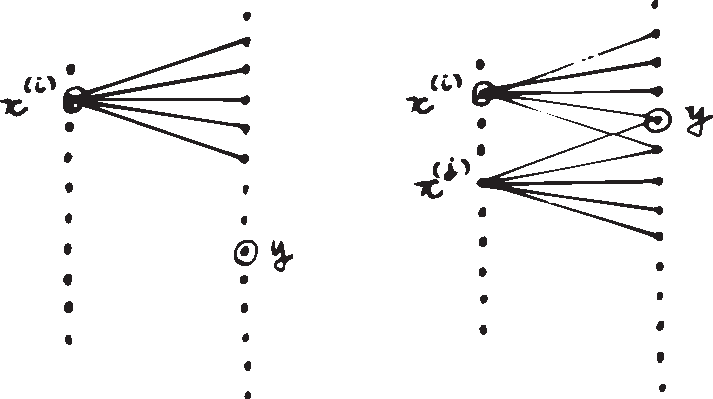
\includegraphics[width=.7\textwidth]{fanchart_2}
% 	\caption{Disjoint output sequences.}\label{fig:disjoint_sequences} \end{figure}
\begin{figure}
	[ht!] \centering
	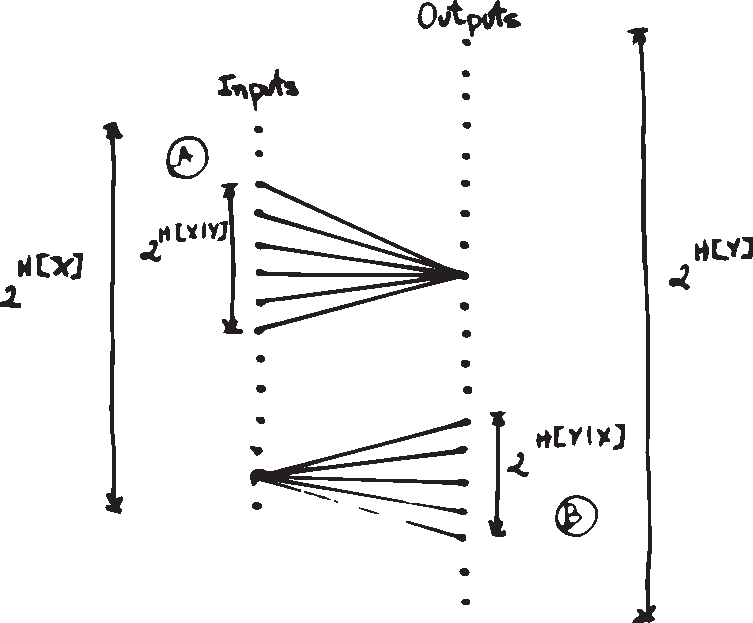
\includegraphics[width=.7\textwidth]{fanchart_1}
	\caption{The need to restrict to the subset of typical inputs and its implications.}\label{fig:fan}
\end{figure}
Take \(\encvec \sim p(\enc^n)\). Recall the source coding theorem (Theorem~\ref{th:source_encoding}), the total number of typical output sequences \(\decvec\) is \(2^{nH[\dec]}\) (see \cref{fig:fan} (B)), all sequences being almost equiprobable. For any sequence \(\encvec\), there are about \(2^{nH[\dec|\enc]}\) probable sequences (see \cref{fig:fan} (A)).

Now we restric ouselves to the subset of the typical inputs such that the correponding typical output sets are disjoint. We can expect the number of non-confusable inputs to be:
\begin{align}
	\leq \frac{2^{nH[\dec]}}{2^{nH[\dec|\enc]}}=2^{n(H[\dec]-H[\dec|\enc])}=2^{nI[\enc;\dec]}
\end{align}

The maximum value of this bound is achieved by the process \(\enc\) that maximises \(I[X;Y]\). Therefore, \(n \max_{p(\encsymb)}I[X;Y]\) is the maximum amount of bits that can be transmitted in \(n\) usages of the channel, which proves the first law of information (see \cref{shannon_laws}):
\begin{align}
	C\text{\tiny{noisy channel}} &= \max_{p(x)} I[\enc,\dec]\label{eq:shannon_1st_law} .
\end{align}

We can rewrite~\eqref{eq:shannon_1st_law} as:
\begin{align}
	C\text{\tiny{noisy channel}} &= \max_{p(x)} (H[\enc]-H[\noise])\label{eq:2nd_law} ,
\end{align}
which states that noise reduces channel capacity. So, this is also a proof for the second law of information (\cref{shannon_laws}).

%
% \subsection{Compression and complexity}
% %


\section{Beyond Shannon's Information}
\subsection{Algorithmic information (Kolmogorov-Chaitin complexity)}
Developed independently by Chaitin, Solomonoff, and Kolmogorov in the 1960s, \emph{algorithmic information} (most commonly known as Kolmogorov complexity) of an object (\eg a message) is the length of the shortest program capable of producing the object as an output\cite{stone:2015}.

For example, in this definition the string 'T6ucFndKEjTyqIGYuXUKqI6fJ6HBRL' is more complex than  'abcabcabcabcabcabcabcabcabcabc'. In python:
\begin{lstlisting}
	"T6ucFndKEjTyqIGYuXUKqI6fJ6HBRL"
\end{lstlisting}
versus
\begin{lstlisting}
	"abc"*10
\end{lstlisting}
If the object is compressable (shorter program), it has more regularity. Thus, there is a relation between complexity and compressibility.
\subsection{Fisher Information}
Let $P_{\theta}$ denote a family of parametric distributions on a space $\XX$ with probability mass or density function given by $p_{\theta}$.

\begin{definition}[Fisher information] The Fisher information $I_{\rvX}(\theta)$ of a random variable $\rvX$ w.r.t. the parameter $\theta$ is the matrix:
	\begin{align}
		[I_{\rvX}(\theta)]_{ij} &:= \E_{\theta} \left[ \nabla_{\theta_i} \log p_{\theta}(\rvX) \cdot  \nabla_{\theta_j} \log p_{\theta}(\rvX)^\top \right] \\
		&= \E_{\theta}\left[ \frac{\partial \ell}{\partial \theta_i} \cdot \frac{\partial \ell}{\partial \theta_j}^\top \right],
	\end{align}
	where $\ell(\rx|\theta)= \log p(\rx|\theta)$ is often called the score function.
\end{definition}
The Fisher information measures the overall sensitivity of the functional relationship $p$ to changes of $\theta$ by weighting the sensitivity at each potential outcome $\rx$ w.r.t $p_{\theta}(\rx)$\cite{maarten:2017}

A common simplification of the Fisher Information Matrix (FIM) is to reduce it to the diagonal:
\begin{align}
	[I_{\rvX}(\theta)]_{i} &:= \E_{\theta} \left[ \nabla_{\theta_i} \log p_{\theta}(\rvX)^2 \right]
\end{align}
\subsection{Shannon vs. Fisher Information}
By using \eqref{eq:ExKL}, \eqref{eq:new_lagrangian} can be rewritten as:
\begin{align*}
  \boldsymbol{\LL(W) = H_{p,q}(D|W) +\beta \KL{\underbrace{q(W|D)}_{\text{training output}}}{\underbrace{p(W)}_{\text{fixed prior}}}}
\end{align*}

In other words, $I(W;D)$ is the divergence of the conditional model distribution $q(W|D)$ and the expected prior averaging all datasets. If, instead, we assume an isotropic gaussian\footnote{An isotropic gaussian is one where the covariance matrix is represented by $\Sigma=\lambda^2 I$.} as the prior, the information in the weights when $W_*$ is minimal, is given by:
\begin{align*}
  \KL{q(W|D)}{p(W)}=\frac{1}{2} \Bigg(\log |F m|+\cancel{\log \lambda^2I} + \cancel{\frac{W_*^2}{\lambda^2I}} \Bigg),
\end{align*}
where the canceled terms are the ones that do not depend on $q(W|D)$ and can be ignored, $\log |F|$ is the log-determinant of Fisher Information Matrix of the weights and $m$ is the number of samples in the dataset.

This is quite interesting as it gives us an analytical and fast calculation of a  bound to $I(W;D)$:
\begin{align}
I(T;X) \leq I(D;W) \leq \log |F(W^*)| \label{bounds}
\end{align}
\section{Connections to Bayesian Inference}
There are countless problems in Science which require that given a limited dataset, preferences be assigned to alternative hypothesis of different complexities. The \textbf{Occam's razor} is the principle that states preference for simple theories. Despite the fact it is often advocated for aesthetic reasons, \citeauthor{mackay:2002} gave a Bayesian explanation for its empirical success that does not depend on any bias towards beauty\cite{mackay:2002}.

Consider the evaluation of the plausability of two alternative theories $\HH_1$ and $\HH_2$, in the light of given evidence ($C$ data). Complex models are capable of making a greater variety of predictions. So, if $\HH_2$ is more complex, it must spread its predictive capability more thinly over the data space $\DD$ than $\HH_1$. Thus, where the gathered data $C$ are compatible with both theories, the simpler $\HH_1$ will be more probable than $\HH_2$ (\cref{modelcomparison}).
\begin{figure}[hbt!]
	\centering
	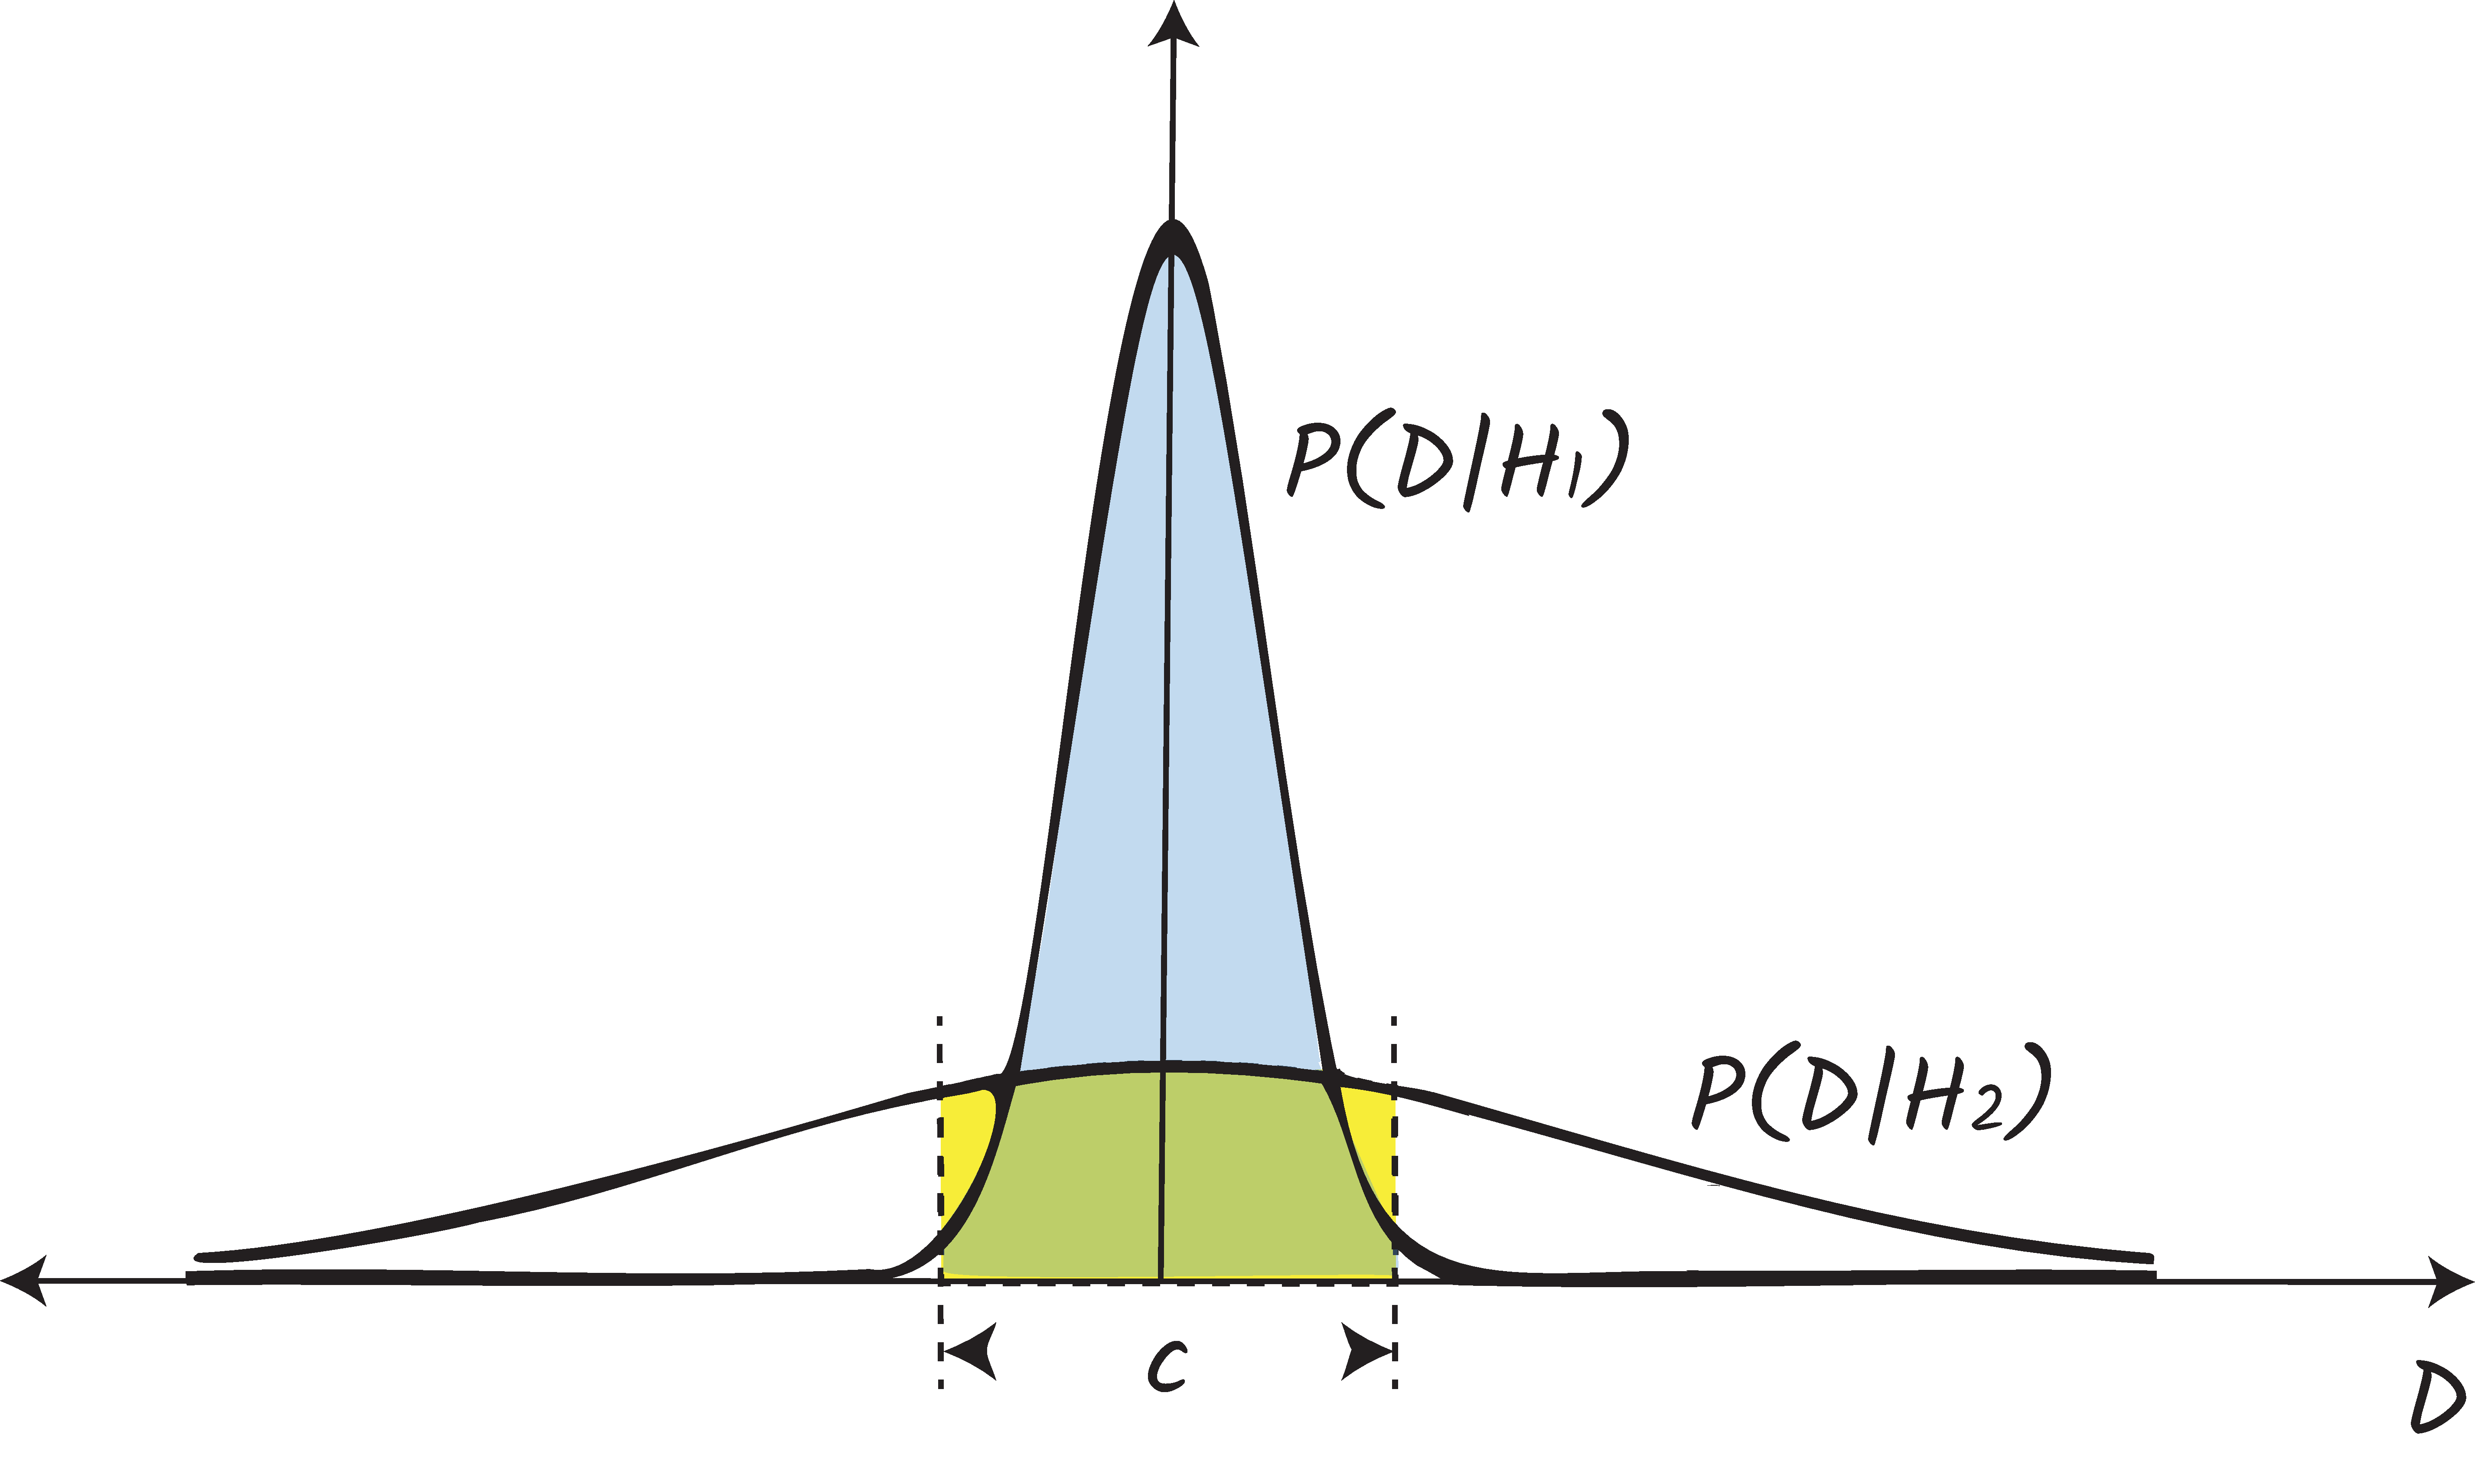
\includegraphics[width=0.75\linewidth]{model_comparison}
	\caption{Comparing models $\HH_1$ and $\HH_2$.}\label{modelcomparison}
	\end{figure}
	\begin{align}
    \frac{P(\HH_1|\DD)}{P(\HH_2|\DD)}&=\frac{P(\HH_1)}{P(\HH_2)}\frac{P(\DD|\HH_1)}{P(\DD|\HH_2)}\\
    \therefore P(\HH_1)&=P(\HH_1),~\text{no model bias} \to  \nonumber\\
		\frac{P(\HH_1|\DD)}{P(\HH_2|\DD)}&=\frac{P(\DD|\HH_1)}{P(\DD|\HH_2)}\label{evidence_comparisson}
   \end{align}

	Simple models make precise predictions, while complex models are capable of making a greater variety of predictions (\cref{modelcomparison}).

	If $\HH_2$ is more complex, it spread its predictive probability over a larger region of the data space $\DD$ than $\HH_1$. When both are compatible with the data, the simpler will turn out more probable than the complexer, despite any model preference.
 \subsection{Quantifying the Occam's razor}
 We already established that we can rank models based by evaluating the evidence$P(\DD|\HH_i)$  (\eqref{evidence_comparisson}) :
 \begin{align}
	P(\DD|\HH_i) = \int P(\DD|\vw, \HH_i) P(\vw|\HH_i) d\vw \label{evidence_integral}
\end{align}
Taking for simplicity the one-dimensional case and applying Laplace's method, we can approximate the evidance by multiplying the peak of $P(\DD|\HH_i)$ by $\sigma_{\vw|\DD}$:
\begin{align}
	\underbrace{P(\DD|\HH_i)}_\text{Evidence} \simeq \underbrace{P(\DD|\vw_{\text{\tiny MP}}, \HH_i)}_\text{Best-fit likelihood} \times \underbrace{P(\vw_{\text{\tiny MP}}|\HH_i) \sigma_{\vw|\DD}}_\text{Occam's factor}
\end{align}
The Occam's factor is the amount by which the accesible volume of $\HH_i$'s hypothesis space collapses when data arrive. This relates to how we measure information (\cref{guessing_game}).
The log of the Occam's factor is a measure of the amount of information we gain about the model's parameteres when data arrive~\cite{mackay:2002}.

The Occam's factor is the basis of \citeauthor{mackay:2002}'s Evidence Framework. The connection was no surprise given that we derived Information from the Bayesian interpretation of Probability (\cref{sec:prob2info}).
\section{Concluding Remarks}

% \begin{fullwidth}
% \cleardoublepage \part{INTERMEZZO}\label{pt:intermezzo}
% \end{fullwidth}
% % !TEX encoding = UTF-8 Unicode
%*********************************************
\chapter{An Information Theoretic Epistemology}\label{ch:it_epistemology}

%*********************************************
\openepigraph{Understanding is Compression}{Gregory Chaitin, [p. 65]\citetitle{chaitin:2006}}
\section{Learning as a conversation with Nature}
\section{PAC-Shannon}
\section{Towards a new theory}


% 

%************************************************
\chapter{The Information Bottleneck Principle}\label{ch:ib}

%************************************************
% \begin{quotation}
% 	\small \textit{ \flushright
% 	Great claims require great evidence.
% 	\flushright --- Carl Sagan \\
% 	\vspace{1cm}}
% \end{quotation}

As we already discussed (see \ref{sec:communication_problem_setting}), Shannon intentionally left out from information theory\footnote{Which Shannon has always referenced as Communication Theory.} issues of meaning or relevance, and focused on the problem of transmitting information.

Contrarily,~\citeauthor{tishby:1999} argue in~\cite{tishby:1999} that lossy source compression provides a natural quantitative approach to the matter of relevance and, therefore, they use Information Theory itself to address relevance.

This chapter will present the Information Bottleneck Principle, the foundation of the emergent theory subject of this dissertation.

The IB principle approach is related to \acf*{RDT}. Hence, first we will briefly overview RDT as~\citeauthor{tishby:1999} describe it~\cite{tishby:1999,slonim:2002}. Then, we will formally present the IB Principle, its problem setting and solution, and show how it can be seen as a special case of \acl{RDT}.

\section{Rate-Distortion Theory: relevance through a distortion function}\label{sec:RDT}
We know from \eqref{eq:shannon_1st_law} that for any rate $R \leq I(X;Y)$ there will be a loss in the reconstructed signal. \acf*{RDT} addresses the problem of determining the rate $R$ that should be communicated over a channel so that the source (input signal $\rvX$) can be approximately reconstructed without exceeding an expected distortion.

\subsection{The \ac{RDT} problem}
\subsubsection{Problem setting}
\begin{enumerate}
	\item Let the discrete random variable $\rvX$ denote the \bt{source} of vectors randomly drawn from a probability distribution \(p(x)\);
	\item Each vector \(x\sim p(x)\) is a \bt{message} you want to transmit among a set of possible messages $\aXX,i.e.\  x \in \aXX$ ;
	\item Let another discrete random variable $\rvZ$ denote\footnote{This compressed representation of $\rvX$ is usually denoted by $\rvZ, \rvT$ or $\hat{\rvX}$ } a compressed \bt{representation} of $\rvX$ ;
	\item This representation is defined by a \bt{channel}\footnote{A noisy channel and a lossy encoder are equivalents.} $p(z|x)$, a stochastic mapping  between each message $x \in \aXX$ to each code $z \in \aZZ$;
	\item The \bt{rate} $R$ is the channel capacity, i.e.\ the average number of bits per element $\rx \in \aXX$ needed to specify a compressed element (code) $\rz \in \aZZ$.
	\item Let $d: \aXX \times \aZZ \to \Real^{+}$ be a function that denote the \bt{distortion measure} between $\rvX$ and its representation $\rvZ$. Examples of distortion measures are the mean square error, $d_{MSE}(x;z)=\langle (x - z)^2 \rangle$ or the Hamming distortion (probability of error) $d_{H}(x,z)=\truth_{[x \neq z]}$.
\end{enumerate}
\subsubsection{Problem Statement}
Given the problem setting above, the \ac*{RDT} problem\footnote{ First defined by Shannon~\cite{shannon:1948}.} is to find the minimal number of bits per symbol (rate $R$) that should be communicated over a channel so that the source $\rvX$ can be approximately reconstructed via a representation $\rvZ$ without exceeding an expected distortion $D$, defined by the distortion function $d(x;z)$.

\subsection{Understanding the \ac*{RDT} problem}
The core of the \ac*{RDT} problem is the need for a good compressed representation of a message. From \eqref{eq:shannon_1st_law}, any rate $I[\rvZ;\rvX] \leq H[\rvX]$ will imply a loss in the reconstructed signal, an expected distortion,  $\langle d(x;z) \rangle$.

As we have seen in \ref{noisy_channel_theorem}, low values of $I[\rvZ;\rvX]$, calculated based on the joint distribution $p(x,y)=p(x)p(z|x)$, imply compact representations, i.e.\ $|\aZZ|$ is small. In the extreme, all messages are translated to the same code: $|\aZZ|=1$ and $I[\rvZ;\rvX]=0$. Contrarily, high values of $I[\rvZ;\rvX]$ imply low compression.  In the extreme, $\rvZ$ simply copies $\rvX$: $I[\rvZ;\rvX]=H[\rvX]$ and $|\aZZ|=|\aXX|$.

If we can compress the input data to any amount of information from $0$ to $H[\rvX]$, what will define the relevance of information is the aditional constraint of the problem: the distortion measure. Given such function, the partitioning of $\rvX$ defined by $p(z|x)$ has the \emph{expected distortion}:
\begin{align}
	\langle d[x;z] \rangle _{p(x,z)} = \sum_{x,z} p(x) p(z|x) d[x;z]
\end{align}

Consequently, we are assuming that the definition of relevance is part of the problem setting. In other words, \ac{RDT} is agnostic on any arbitrary choice of the distortion function. This choice, nevertheless, determines the relevant features of the signal\footnote{About MLT, the same can be said of a learning algorithm loss function, which determines what is relevant to be learned.} and should be somehow related to the task we want to perform with the input. An arbitrary distortion function is, in fact, an arbitrary feature selection\cite{tishby:1999}.

As we will se further (\ref{sec:IB_principle},~\citeauthor{tishby:1999}~\cite{tishby:1999} propose a way to cope with this potential pitfall.

\subsection{\ac*{RDT} as a variational problem}\label{RDT problem}
\begin{definition}
	 The \bt{rate-distortion function}, denoted by $R(D)$ is defined as:
	 \begin{align}
		R(D) \equiv \underset{p(z|x):~ \langle d(x;z) \rangle \leq D}{\min} I[\rvZ;\rvX]. \label{rate-distortion function}
	\end{align}
\end{definition}

Therefore, $R(D)$ is the minimal achievable rate among all normalized conditional distributions, $p(z|x)$, for which the distortion constraint is satisfied. The \emph{rate-distortion function} is a non-increasing convex function of D in the \emph{distortion-compression plane} (\cref{fig:distortion-compression-plane}\footnote{We will explain what $\beta$ means later.})~\cite{cover:2006}.

	\begin{figure}
		[htb] \centering
		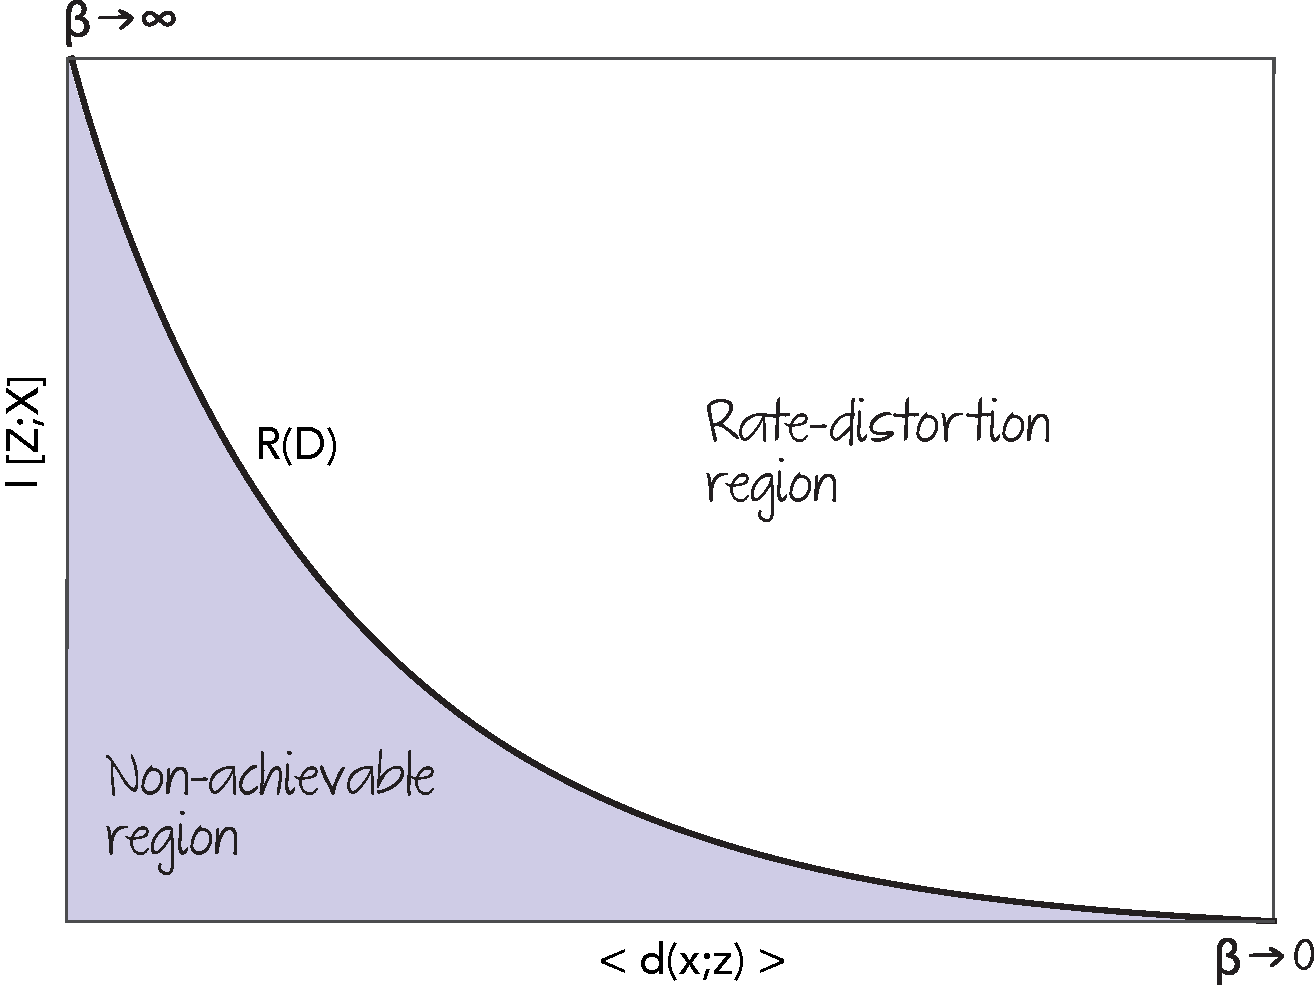
\includegraphics[width=
		.7\textwidth]{distortion-compression}
		\caption{The rate-distortion function, $R(D)$, in the distortion-compression plane.}
	\label{fig:distortion-compression-plane}
	\end{figure}
The region above the curve corresponds to all achievable \emph{distortion-compression} pairs, while below the curve is the non-achievable region. Let $\{D, I_{\rvX}\}$ be a \emph{distortion-compression} pair, if it is in the achievable region there is a representation $\rvZ$ with a compression level $I[\rvZ;\rvX]=\Ix$ and an expected distortion of at most $D$. If it is in the non-achievable region, there is no such representation $\rvZ$. This limit on the achievability of representations is a direct consequence of Shannon's laws (\ref{shannon_laws}).

Instead of solving the minimization problem in \eqref{rate-distortion function} exactly, the problem is usually approximated by the following Lagrangian relaxation functional:
\begin{align}
	\mathcal{F}[p(z|x)] = I[\rvZ;\rvX] + \beta \langle d(x;z) \rangle_{p(x,z)},
\end{align}
under the normalization constraint $\sum_z p(z|x)=1, \forall x \in \aXX$.

\begin{theorem}\label{thrm:RDT solution}
	The solution of the variational problem~\cite{tishby:1999}
	\begin{align}
		\frac{\partial \mathcal{F}}{\partial p(z|x)}=0,
	\end{align}
	for normalized distributions $p(z|x)$ is given by the exponential form
	\begin{align}
		p(z|x) = \frac{p(z)}{Z(x,\beta)}\exp (-\beta ~d(x;z)),\label{exponential-form}
	\end{align}
	where $Z$ is the normalization factor (partition function).  The Lagrange multiplier $\beta$ is positive and
	\begin{align}
		\frac{\partial R}{\partial D} = - \beta.
	\end{align}
\end{theorem}
This is an implicit solution\footnote{Implicit solution means a solution in which dependent variable is not separated.} as $p(z)$ on the right-hand side of \eqref{exponential-form} depends on $p(z|x)$\footnote{$p(z)=\sum_{x,z} p(z|x)~p(z)$}.

\section{The IB Principle: relevance through a target variable}\label{sec:IB_principle}
The problem of extracting a relevant summary of data depends on a suitable definition of relevance. The main weakness of the \ac{RDT} approach is that it addresses relevance through a distortion function that is not related to a specific task at hand.

The \bt{IB Principle}, suggested by \citeauthor{tishby:1999}\cite{tishby:1999} introduces an alternative approach: defining a ``target'' variable is simpler and more direct than defining a distortion measure.

For example, in speech compression\footnote{By the time of~\cite{tishby:1999} publication, Tishby was working on speech-related problems.}, any compression beyond the signal's entropy cannot be perfectly reconstructed; it is a lossy compression. On the other hand, a transcript has orders of magnitude lower entropy than the acoustic waveform, which means that for the task of understanding what has been transmitted, it is possible to compress the signal \emph{much} further without losing any information about meaning~\cite{tishby:1999}.

\begin{figure}
	[htb] \centering
	\includegraphics[width=
	\textwidth]{ib_setting}
	\caption{The IB problem setting.}\label{fig:ib_problem_setting}
\end{figure}

In many situations, we have access to an additional variable that determines what is relevant. If we want to recognize cats in pictures, maybe we do not need a 360~kb picture as depicted on the left in \cref{fig:ib_problem_setting}; the 5~kb representation on the right may suffice. The exact representation would not be sufficient for the task of recognizing the breed of the cat, in any case. Relevance is task-dependent.


\subsection{The IB Problem Setting}\label{ib_problem_setting}
\subsubsection{Definitions}
\begin{enumerate}
	\item Let $\rvX$ be a random variable that denotes the \textbf{Source} \footnote{The IB problem is a one-shot coding problem, the operations are performed letterwise~\cite{zaidi:2020}.} of \textbf{messages} $\rx \in \sA_{\rvX}$;
	\item Let $\rvY$ be a random \textbf{relevant variable}  (or \textbf{Target}) which defines the intended meaning $p(y|x)$ of the message $x$;
	\item Let $\rvZ$ be an \textbf{information bottleneck} variable, the representation, that obeys the Markov chain $\rvY \leftrightarrow \rvX \leftrightarrow \rvZ$;
	\item Let the conditional p.d.f $p(z|x)$ be the \textbf{encoder}, \ie a stochastic mapping from each value of $x \in \sA_{\rvX}$ to a codeword $z \in \sA_{\rvZ}$;
	\item $I(\rvX ; \rvZ)$ is the \textbf{rate} (or compression level) of the encoder, and reflects how much the bottleneck representation  $\rvZ$ compresses $\rvX$;
	\item Let the conditional p.d.f $p(y|z)$ be the \textbf{decoder}, \ie a stochastic mapping from each value of $z \in \sA_{\rvZ}$ to a prediction $\hat{y} \in \hat{\rvY}$;
	\item $I(\rvZ ; \rvY)$ is the \textbf{relevant information} that the compressed representation $\rvZ$ keeps from the label variable $\rvY$;
\end{enumerate}

  \subsubsection{Assumptions}\label{assumptions}
  \begin{enumerate}
    [i.]
    \item The random variables $\rvX$, $\rvY$ and $\rvZ$ are discrete;
    \item $\sA_{\rvX}$, $\sA_{\rvY}$ and $\sA_{\rvZ}$ are finite sets;
    \item $\rvX$ and $\rvY$ are dependent and the joint distribution $p(\rvX=x, \rvY=y)$ is known;
		\item The source $\rvX$ is an ergodic process\footnote{The \emph{ergodic} property means statistical homogeneity~\cite{shannon:1949}:~ its statistical properties can be deduced from a single, sufficiently long, random sample of the process.}, therefore $x \sim p(x)$ are not necessarily mutually independent.
		\item The encoder and the decoder are stochastic mappings \footnote{Notice that given the Markov chain $\rvY \leftrightarrow \rvX \leftrightarrow \rvZ$, due to reparemetrization invariance (Theorem \ref{th:reparemetrisation_invariance}), a deterministic mapping of the data does not throw out information, i.e. \ let $f:\aXX \to \aYY$ be deterministic, $I[f(\rvX);\rvY]=\IXY$.}.
  \end{enumerate}
\subsubsection{Problem statement}
% The \emph{information bottleneck} consists of finding a representation $\rvZ$ for $\rvX$ that preserves the maximum information about $\rvY$, squeezing the information that $\rvX$ contains on $\rvY$ through a \emph{bottleneck} $\rvZ$ defined by a limited set of codewords $\sA_{\rvZ}$.
The \emph{information bottleneck problem} consists of finding an encoder $p(z|x)$ that produces a codebook  $\rvZ$ that compress $\rvX$ as much as possible, i.e.\ $I(\rvX ; \rvZ)$ is minimal, while keeping the \emph{relevant information} of $\rvX$ for the task of predicting $\rvY$, $I(\rvZ;\rvY)$. In other words, the representation $\rvZ$ acts like a \bt{bottleneck} that "squeezes" the relevant information that $\rvX$ contains about the target $\rvY$ in a compressed form, hence the name "information bottleneck".
\subsection{Relation to other Information Theory Problems}
Connections between problems allow extending ideas from one setup to another. In this regard, the IB problem is closely related to other coding problems like the \emph{Indirect} or \emph{Remote Source-coding problem}, also known as the \emph{CEO Problem}, and the \emph{privacy funnel problem}\cite{zaidi:2020}.
\subsection{Relation to Minimum Sufficient Statistics}
As we have said before,  a \bt{statistic} is a function of a random variable that does not depend on its parameters. In the IB problem, the target variable is what we want to predict. $\rvY$ acts as a parameter of $\rvX$ and  $\rvZ \ind \rvY$. Thus, \emph{the representation $\rvZ$ is a statistic of $\rvX$}.

For $\rvZ$ to be a \bt{sufficient statistic} of $\rvX$ w.r.t. $\rvY$, it must preserve all relevant information in $\rvX$, $I[Y;X]=I[Z;X]$. In other words, no other statistic of $\rvX$ can provide any additional information as to the value of $\rvY$ than $\rvZ$ does.

The representation is \bt{minimal} if it is the smallest among all possible representations.

Therefore, we can say that the information bottleneck is the problem of finding the \emph{minimum sufficient statistics} of the random variable $\rvX$ w.r.t $\rvY$, and therefore, IB Lagrangian gives the minimum approximately sufficient statistic.
\section{The IB functional}\label{sec:ib_functional}
As in {RDT}, the compactness of the representation is measured by $I[\rvZ;\rvX]$.  The distortion upper-bound constraint, however, is replaced by a lower bound constraint over the \emph{relevant information}, $I[\rvZ;\rvY]$\cite{slonim:2002}.

\begin{definition} The \textbf{IB functional}, also know as the \emph{IB Curve} or \emph{relevance-compression function}, is the functional that express the IB problem\cite{bachrach:2003}:
\begin{align}
	R^{(\text{IB})}(I_{\rvY}) &= \underset{p(z|x):~ I[\rvZ;\rvY]\geq I_{\rvY}}{\min} I[\rvZ;\rvX],\\
	\text{or alternatively:} \nonumber                                              \\
	I_{\rvY}^{(\text{IB})}(R)&= \underset{p(z|x):~ I[\rvZ;\rvX]\leq R}{\max} I[\rvZ;\rvY],
\end{align}
where the random variables form a Markov chain $\rvY \leftrightarrow  \rvX \leftrightarrow  \rvZ$ and the minimization is over all the normalized conditional distributions $p(z|x)|\sum_x p(z|x)=1$ for which the constraint is satisfied.
\end{definition}
A straighforward observation is that the Markovian relation characterizes $p(z)$ and $p(y|z)$ through\cite{slonim:2002}
\begin{align}
	\begin{cases}
		p(z) = \sum_{x,y} p(x,y,z) = \sum_x p(x)p(z|x)  \\
		p(y|z) = \frac{1}{p(z)}\sum_x p(x,y,z) = \frac{1}{p(z)}\sum_x p(x,y) p(z|x).\label{observation}
	\end{cases}
\end{align}

Moreover, the plane where the horizontal axis corresponds to $I[\rvZ;\rvX]$ and the vertical axis to $I[\rvZ;\rvY]$, named \bt{information plane} (see Figure \cref{fig:information-plane}), is the natural equivalent to the distortion-compression plane in \acl{RDT} (see \cref{fig:distortion-compression-plane})\footnote{The horizontal and vertical axis are inverted for consistency with how~\cite{tishby:2015} define the information plane. Therefore, whereas the rate-distortion function is convex, the IB curve is concave.}. Let the pair ${R, \Iy}$ denote some levels of compression and relevant information, respectively. If this pair is located below the curve, there is some compressed representation $\rvZ$ with a compression level $R=I[\rvZ;\rvX]$ and relevant information $\Iy=I[\rvZ;\rvY]$. The points laying on the IB Curve are the optimal representations for a certain level of relevant-information (or precision) $\Iy$ or a certain level of compression (or complexity) $R$.


\begin{figure}
	[htb] \centering
	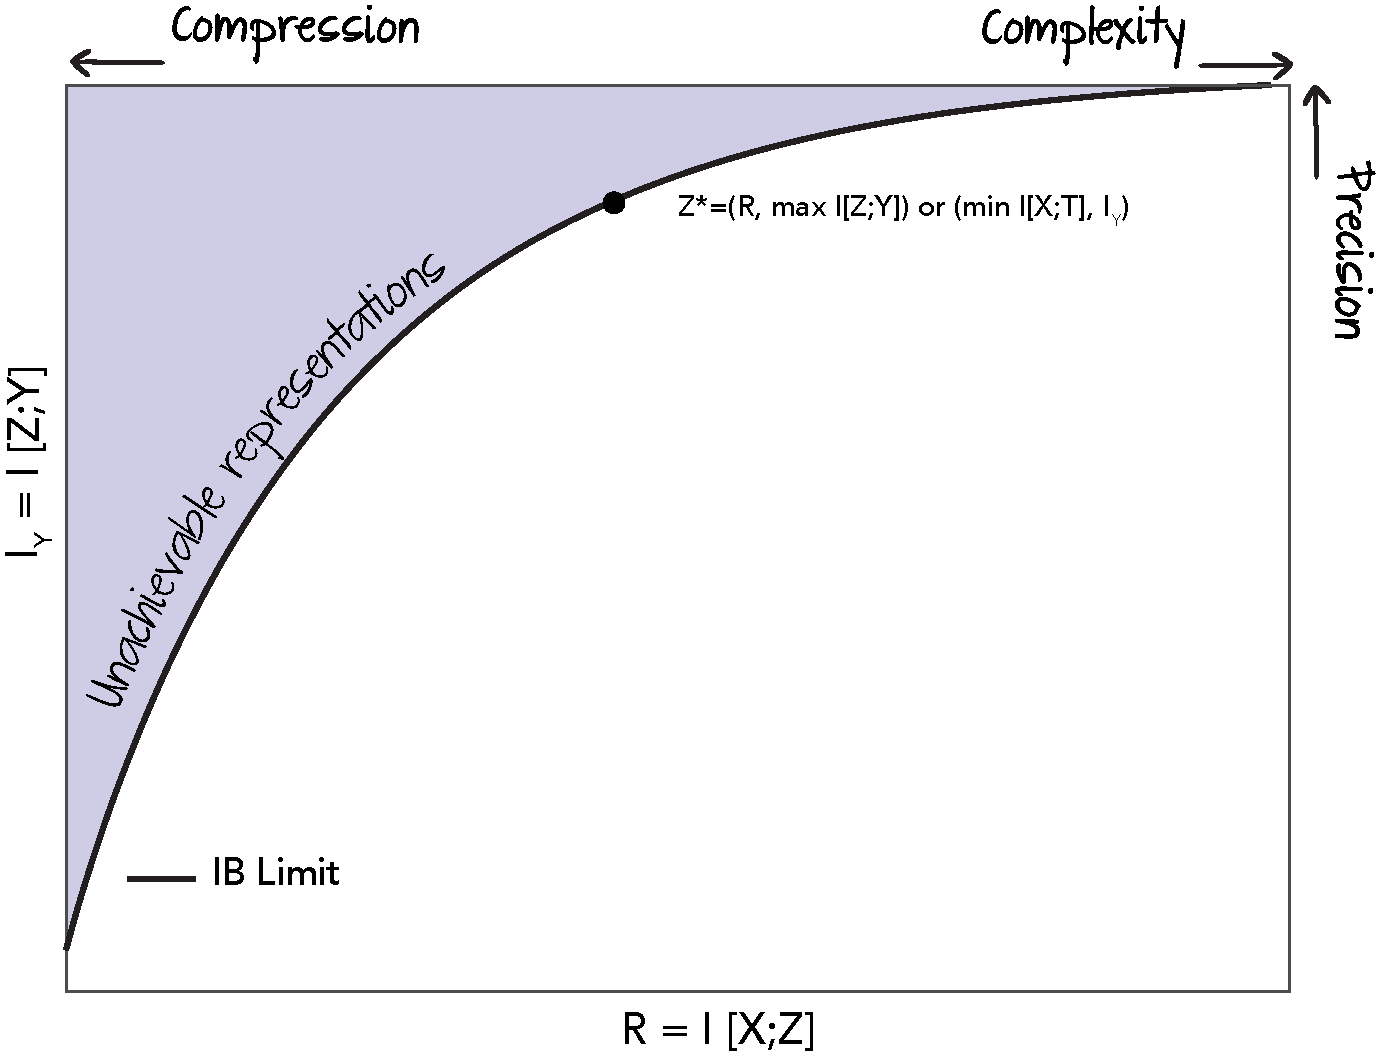
\includegraphics[width=
	.7\textwidth]{information-plane}
	\caption{The IB Curve, $R^{\text{(IB)}}(D)$, in the information plane.}\label{fig:information-plane}
\end{figure}
\section{The IB Problem Relaxation}\label{sec:ib_problem_relaxation}
The Lagrangian relaxation of the IB functional is also a variational problem:

\begin{align}
	\LH_{\beta}^{\text{(IB)}}[p(z|x)] = \IZX - \beta \IZY, \label{IB_Lagrangian}
\end{align}
where $\beta$ is the Lagrangian multiplier attached to the constrained relevant information\cite{tishby:1999}.

At $\beta=0$, no feature of the signal is relevant, and all messages are quantized (compressed) to a single point. At $\beta=\infty$, the solution is pushed toward arbitrarily detailed quantization (no compression). "By varying the (only) parameter, $ \beta$, one can explore the tradeoff between the preserved meaningful information and compression at various resolutions"\cite{tishby:1999}.
% Relevant information
% For each value $x \in X$ we seek a stochastic mapping to a codeword $z$ in a codebook $Z$, characterized by the p.d.f. $p(z|x)$, which induces a soft partitioning of $X$ in which each block is associated with one element $z \in Z$, with probability \[p(z)=\sum_x p(x) p(z|x).\]

% The average volume of elements of $X$ mapped to the same codeword is $2ˆ{H(X|Z)}$, where
% \[ H(X|Z)= - \sum_{x \in X}p(x) \sum_{z \in Z} p(z|x) \log p(z|x) \] is the conditional entropy of $X$ given $Z$.

Unlike the case of the \cref{RDT problem}, in the IB problem, the constraint on the meaningful information is \emph{nonlinear} in the mapping  $p(z|x)$, and it is a much harder variational problem. Notably, there is an analytical solution for \Eqref{IB_Lagrangian}. For the sake of clarity, before deriving this exact solution, we will show how IB can be seen as a particular case of \ac*{RDT}. This development will further help us to derive the analytical solution easily.

\section{IB problem as a special case of the RDT problem}
From the \acf{DPI}, \(I[\rvX;\rvY] \geq I[\rvZ;\rvY]\). Therefore, we can consider that the relevant information of $\rvX$ not captured by the representation $\rvZ$ is a natural choice for the expected distortion, as it represents a distortion in bits.
\begin{align}
	\langle d[x;z] \rangle = I[\rvX;\rvY]-I[\rvZ;\rvY]\geq 0
\end{align}
From this definition, we can derive the following theorem:
\begin{theorem}
If $\langle d[x;z] \rangle_{p(x,z)}=I[\rvX;\rvY]-I[\rvZ;\rvY]$, then $\\d[x;z] = \KL(p(y|x)~||~p(y|z))$.
\end{theorem}
\begin{proof}
	\begin{align}
		&\langle d[x;z] \rangle_{p(x,z)} =I[\rvX;\rvY]-I[\rvZ;\rvY]\nonumber\\
		&=\sum_{x,y} p(x, y) \log \frac{p(x,y)}{p(x) p(y)} - \sum_{z,y} p(z, y) \log \frac{p(z,y)}{p(z) p(y)}.
	\end{align}
	Since $p(a,b) = p(b|a) p(a)$, we have:
	\begin{align}
		=&\sum_{x,y} p(y|x) p(x) \log \frac{p(y|x)\cancel{p(x)}}{ \cancel{p(x)}p(y)} -\sum_{z,y} p(y|z) p(z) \log \frac{p(y|z)\cancel{p(z)}}{ \cancel{p(z)}p(y)}.
	\end{align}
	From \eqref{observation} :
	\begin{align}
		=&\sum_{x,y} p(y|x) p(x) \log \frac{p(y|x)}{ p(y)} - \sum_{z,y,x} \frac{p(y|x) p(z|x) p(x) \cancel{p(z)}}{\cancel{p(z)}}~\log \frac{p(y|z)}{ p(y)}\\
		=&\sum_{x,y} p(y|x) p(x) \log \frac{p(y|x)}{ p(y)} - \sum_{z,y,x} p(y|x) p(z,x)~\log \frac{p(y|z)}{ p(y)}.
	\end{align}
	From the normalization constraint, $\sum_{z} p(z|x)=1$:
	\begin{align}
		=&\cancelto{\sum_{z} p(z|x)}{1} \cdot \sum_{x,y} p(x) p(y|x) \log \frac{p(y|x)}{ p(y)} - \sum_{z,y,x} p(y|x) p(z,x)\log \frac{p(y|z)}{ p(y)}\\
		=&\sum_{z,x} p(z|x)p(x) \left[\sum_{y}  p(y|x) \log \frac{p(y|x)}{ p(y)}\right] - \sum_{z,x} p(x,z) \left[ \sum_{y} p(y|x) \log \frac{p(y|z)}{ p(y)}\right]\\
		=&\sum_{z,x} p(x,z) \left[\sum_{y}  p(y|x) \left(\log \frac{p(y|x)}{ p(y)}- \log \frac{p(y|z)}{ p(y)}\right)\right]\\
		=&\sum_{z,x} p(x,z) \left[\sum_{y}  p(y|x) \left(\log \frac{p(y|x) \cancel{p(y)}}{ \cancel{p(y)} p(y|z)}\right)\right]\\
		=&\E_{p(z,x)}  \KL{\left(~p(y|x)~ ||~ p(y|z)~ \right)}.
	\end{align}
	Therefore
	\begin{align}
		\langle d[x;z] \rangle_{p(x,z)} &= \langle \KL{\left(~p(y|x)~ ||~ p(y|z)~ \right)} \rangle_{p(x,z)}\\
		d[x;z] &= \KL{\left(~p(y|x)~ ||~ p(y|z)~ \right)}
	\end{align}
\end{proof}

\section{Information Bottleneck Solution}% Analytical solution

Theorem \ref{thrm:RDT solution} characterizes the general form of the optimal solution to the rate-distortion problem. As we showed that the IB problem could be seen as a special case of the RDT problem, the IB solution is straightforward:\footnote{The analytical solution to the IB problem is sometimes called the self-consistent equations.}
\begin{theorem}\label{thrm:IB solution}
	The analytical solution of the variational problem
	\begin{align}
		\frac{\partial \mathcal{L}_{\beta}^{\text{(IB)}}[p(z|x)]}{\partial p(z|x)} = 0,
	\end{align}
	for normalized distributions $p(z|x)$ is given by the exponential form
	\begin{align}
		\begin{cases}
		p(z|x) &= \frac{p(z)}{Z(x,\beta)}\exp (-\beta ~\KL{\left(~p(y|x)~ ||~ p(y|z)~ \right)}),\\
		p(z) &= \sum_{x,y} p(x,y,z) = \sum_x p(x)p(z|x)  \\
		p(y|z) &= \frac{1}{p(z)}\sum_x p(x,y,z) = \frac{1}{p(z)}\sum_x p(x,y) p(z|x).
		\end{cases}
	\end{align}
	where $Z$ is the normalization factor (partition function).  The Lagrange multiplier $\beta$ is positive and
	\begin{align}
		\beta = \frac{\partial I[Z;Y]}{\partial I{Z;X}}.
	\end{align}
\end{theorem}
\begin{proof}
	Apply $d[x;z] = \KL{\left(~p(y|x)~ ||~ p(y|z)~ \right)}$ to theorem \ref{thrm:RDT solution}.
\end{proof}
% \ctparttext{Where you can put some informational part preamble text here.}
% \renewcommand{\thepart}{\roman{part}}
% \@addtoreset{part}{thepart}
% \setcounter{part}{2}
% \setcounter{thepart}{2}
% \begin{fullwidth}
% \cleardoublepage \part{The emergence of a theory}\label{pt:emergence_of_theory}
% \end{fullwidth}
% 

%************************************************
\chapter{The Information Bottleneck Principle}\label{ch:ib}

%************************************************

As we already discussed (\cref{sec:communication_problem_setting}), Shannon intentionally left out from information theory\footnote{Which Shannon has always referenced as Communication Theory.} issues of meaning or relevance, and focused on the problem of transmitting information.

Contrarily,~\citeauthor{tishby:1999} argue in~\cite{tishby:1999} that lossy source compression provides a natural quantitative approach to the matter of relevance and, therefore, they use Information Theory itself to address relevance.

This chapter will present the Information Bottleneck Principle, the foundation of the emergent theory subject of this dissertation.

The IB principle approach is related to \acf*{RDT}. Hence, first we will briefly overview RDT as~\citeauthor{tishby:1999} describe it~\cite{tishby:1999,slonim:2002}. Then, we will formally present the IB Principle, its problem setting and solution, and show how it can be seen as a special case of \acl{RDT}.

\section{Rate-Distortion Theory: relevance through a distortion function}\label{sec:RDT}
We know from \cref{eq:shannon_1st_law} that for any rate $R \leq I(X;Y)$ there will be a loss in the reconstructed signal. \acf*{RDT} addresses the problem of determining the rate $R$ that should be communicated over a channel so that the source (input signal $\rvX$) can be approximately reconstructed without exceeding an expected distortion.

\subsection{The \ac{RDT} problem}
\subsubsection{Problem setting}
\begin{enumerate}
	\item Let the discrete random variable $\rvX$ denote the \textbf{source} of vectors randomly drawn from a probability distribution \(p(x)\);
	\item Each vector \(x\sim p(x)\) is a \textbf{message} you want to transmit among a set of possible messages $\aXX,i.e.\  x \in \aXX$ ;
	\item Let another discrete random variable $\rvZ$ denote\footnote{This compressed representation of $\rvX$ is usually denoted by $\rvZ, \rvT$ or $\hat{\rvX}$ } a compressed \textbf{representation} of $\rvX$ ;
	\item This representation is defined by a \textbf{channel}\footnote{A noisy channel and a lossy encoder are equivalents.} $p(z|x)$, a stochastic mapping  between each message $x \in \aXX$ to each code $z \in \aZZ$;
	\item The \textbf{rate} $R$ is the channel capacity, i.e.\ the average number of bits per element $\rx \in \aXX$ needed to specify a compressed element (code) $\rz \in \aZZ$.
	\item Let $d: \aXX \times \aZZ \to \Real^{+}$ be a function that denote the \textbf{distortion measure} between $\rvX$ and its representation $\rvZ$. Examples of distortion measures are the mean square error, $d_{MSE}(x;z)=\langle (x - z)^2 \rangle$ or the Hamming distortion (probability of error) $d_{H}(x,z)=\truth_{[x \neq z]}$.
\end{enumerate}
\subsubsection{Problem Statement}
Given the problem setting above, the \ac*{RDT} problem\footnote{ First defined by Shannon~\citeonly{shannon:1948}.} is to find the minimal number of bits per symbol (rate $R$) that should be communicated over a channel so that the source $\rvX$ can be approximately reconstructed via a representation $\rvZ$ without exceeding an expected distortion $D$, defined by the distortion function $d(x;z)$.

\subsection{Understanding the \ac*{RDT} problem}
The core of the \ac*{RDT} problem is the need for a good compressed representation of a message. From \cref{eq:shannon_1st_law}, any rate $I[\rvZ;\rvX] \leq H[\rvX]$ will imply a loss in the reconstructed signal, an expected distortion,  $\langle d(x;z) \rangle$.

As we have seen in \cref{noisy_channel_theorem}, low values of $I[\rvZ;\rvX]$, calculated based on the joint distribution $p(x,y)=p(x)p(z|x)$, imply compact representations, i.e.\ $|\aZZ|$ is small. In the extreme, all messages are translated to the same code: $|\aZZ|=1$ and $I[\rvZ;\rvX]=0$. Contrarily, high values of $I[\rvZ;\rvX]$ imply low compression.  In the extreme, $\rvZ$ simply copies $\rvX$: $I[\rvZ;\rvX]=H[\rvX]$ and $|\aZZ|=|\aXX|$.

If we can compress the input data to any amount of information from $0$ to $H[\rvX]$, what will define the relevance of information is the aditional constraint of the problem: the distortion measure. Given such function, the partitioning of $\rvX$ defined by $p(z|x)$ has the \emph{expected distortion}:
\begin{align}
	\langle d[x;z] \rangle _{p(x,z)} = \sum_{x,z} p(x) p(z|x) d[x;z]
\end{align}

Consequently, we are assuming that the definition of relevance is part of the problem setting. In other words, \ac{RDT} is agnostic on any arbitrary choice of the distortion function. This choice, nevertheless, determines the relevant features of the signal\footnote{About MLT, the same can be said of a learning algorithm loss function, which determines what is relevant to be learned.} and should be somehow related to the task we want to perform with the input. An arbitrary distortion function is, in fact, an arbitrary feature selection~\cite{tishby:1999}.

As we will se further (\cref{sec:IB_principle}),~\citeauthor{tishby:1999}~\cite{tishby:1999} propose a way to cope with this potential pitfall.

\subsection{\ac*{RDT} as a variational problem}\label{RDT problem}
\begin{definition}
	 The \textbf{rate-distortion function}, denoted by $R(D)$ is defined as:
	 \begin{align}
		R(D) \equiv \underset{p(z|x):~ \langle d(x;z) \rangle \leq D}{\min} I[\rvZ;\rvX]. \label{rate-distortion function}
	\end{align}
\end{definition}

Therefore, $R(D)$ is the minimal achievable rate among all normalized conditional distributions, $p(z|x)$, for which the distortion constraint is satisfied. The \emph{rate-distortion function} is a non-increasing convex function of D in the \emph{distortion-compression plane} (\cref{fig:distortion-compression-plane}\footnote{We will explain what $\beta$ means later.})~\cite{cover:2006}.

\blockfigure{distortion-compression-plane}{1}{The rate-distortion function, $R(D)$, in the distortion-compression plane.}

The region above the curve corresponds to all achievable \emph{distortion-compression} pairs, while below the curve is the non-achievable region. Let $\{D, I_{\rvX}\}$ be a \emph{distortion-compression} pair, if it is in the achievable region there is a representation $\rvZ$ with a compression level $I[\rvZ;\rvX]=\Ix$ and an expected distortion of at most $D$. If it is in the non-achievable region, there is no such representation $\rvZ$. This limit on the achievability of representations is a direct consequence of Shannon's laws (\ref{shannon_laws}).

Instead of solving the minimization problem in \eqref{rate-distortion function} exactly, the problem is usually approximated by the following Lagrangian relaxation functional:
\begin{align}
	\mathcal{F}[p(z|x)] = I[\rvZ;\rvX] + \beta \langle d(x;z) \rangle_{p(x,z)},
\end{align}
under the normalization constraint $\sum_z p(z|x)=1, \forall x \in \aXX$.

\begin{theorem}\label{thrm:RDT solution}
	The solution of the variational problem~\cite{tishby:1999}
	\begin{align}
		\frac{\partial \mathcal{F}}{\partial p(z|x)}=0,
	\end{align}
	for normalized distributions $p(z|x)$ is given by the exponential form
	\begin{align}
		p(z|x) = \frac{p(z)}{Z(x,\beta)}\exp (-\beta ~d(x;z)),\label{exponential-form}
	\end{align}
	where $Z$ is the normalization factor (partition function).  The Lagrange multiplier $\beta$ is positive and
	\begin{align}
		\frac{\partial R}{\partial D} = - \beta.
	\end{align}
\end{theorem}
This is an implicit solution\footnote{Implicit solution means a solution in which dependent variable is not separated.} as $p(z)$ on the right-hand side of \cref{exponential-form} depends on $p(z|x)$\footnote{$p(z)=\sum_{x,z} p(z|x)~p(z)$}.

\section{The IB Principle: relevance through a target variable}\label{sec:IB_principle}
The problem of extracting a relevant summary of data depends on a suitable definition of relevance. The main weakness of the \ac{RDT} approach is that it addresses relevance through a distortion function that is not related to a specific task at hand.

The \textbf{IB Principle}, suggested by \citeauthor{tishby:1999}\cite{tishby:1999} introduces an alternative approach: defining a ``target'' variable is simpler and more direct than defining a distortion measure.

For example, in speech compression\footnote{By the time of~\citeonly{tishby:1999} publication, Tishby was working on speech-related problems.}, any compression beyond the signal's entropy cannot be perfectly reconstructed; it is a lossy compression. On the other hand, a transcript has orders of magnitude lower entropy than the acoustic waveform, which means that for the task of understanding what has been transmitted, it is possible to compress the signal \emph{much} further without losing any information about meaning~\cite{tishby:1999}.

\blockfigure{ib_problem_setting}{1}{The IB problem setting.}

In many situations, we have access to an additional variable that determines what is relevant. If we want to recognize cats in pictures, maybe we do not need a 360~kb picture as depicted on the left in \cref{fig:ib_problem_setting}; the 5~kb representation on the right may suffice. The exact representation would not be sufficient for the task of recognizing the breed of the cat, in any case. Relevance is task-dependent.


\subsection{The IB Problem Setting}\label{ib_problem_setting}
\subsubsection{Definitions}
\begin{enumerate}
	\item Let $\rvX$ be a random variable that denotes the \textbf{Source} \footnote{The IB problem is a one-shot coding problem, the operations are performed letterwise~\citeonly{zaidi:2020}.} of \textbf{messages} $\rx \in \sA_{\rvX}$;
	\item Let $\rvY$ be a random \textbf{relevant variable}  (or \textbf{Target}) which defines the intended meaning $p(y|x)$ of the message $x$;
	\item Let $\rvZ$ be an \textbf{information bottleneck} variable, the representation, that obeys the Markov chain $\rvY \leftrightarrow \rvX \leftrightarrow \rvZ$;
	\item Let the conditional p.d.f $p(z|x)$ be the \textbf{encoder}, \ie a stochastic mapping from each value of $x \in \sA_{\rvX}$ to a codeword $z \in \sA_{\rvZ}$;
	\item $I(\rvX ; \rvZ)$ is the \textbf{rate} (or compression level) of the encoder, and reflects how much the bottleneck representation  $\rvZ$ compresses $\rvX$;
	\item Let the conditional p.d.f $p(y|z)$ be the \textbf{decoder}, \ie a stochastic mapping from each value of $z \in \sA_{\rvZ}$ to a prediction $\hat{y} \in \hat{\rvY}$;
	\item $I(\rvZ ; \rvY)$ is the \textbf{relevant information} that the compressed representation $\rvZ$ keeps from the label variable $\rvY$;
\end{enumerate}

  \subsubsection{Assumptions}\label{assumptions}
  \begin{enumerate}
    [i.]
    \item The random variables $\rvX$, $\rvY$ and $\rvZ$ are discrete;
    \item $\sA_{\rvX}$, $\sA_{\rvY}$ and $\sA_{\rvZ}$ are finite sets;
    \item $\rvX$ and $\rvY$ are dependent and the joint distribution $p(\rvX=x, \rvY=y)$ is known;
		\item The source $\rvX$ is an ergodic process\footnote{The \emph{ergodic} property means statistical homogeneity~\citeonly{shannon:1949}:~ its statistical properties can be deduced from a single, sufficiently long, random sample of the process.}, therefore $x \sim p(x)$ are not necessarily mutually independent.
		\item The encoder and the decoder are stochastic mappings \footnote{Notice that given the Markov chain $\rvY \leftrightarrow \rvX \leftrightarrow \rvZ$, due to reparemetrization invariance (Theorem \ref{th:reparemetrisation_invariance}), a deterministic mapping of the data does not throw out information, i.e. \ let $f:\aXX \to \aYY$ be deterministic, $I[f(\rvX);\rvY]=\IXY$.}.
  \end{enumerate}
\subsubsection{Problem statement}
% The \emph{information bottleneck} consists of finding a representation $\rvZ$ for $\rvX$ that preserves the maximum information about $\rvY$, squeezing the information that $\rvX$ contains on $\rvY$ through a \emph{bottleneck} $\rvZ$ defined by a limited set of codewords $\sA_{\rvZ}$.
The \emph{information bottleneck problem} consists of finding an encoder $p(z|x)$ that produces a codebook  $\rvZ$ that compress $\rvX$ as much as possible, i.e.\ $I(\rvX ; \rvZ)$ is minimal, while keeping the \emph{relevant information} of $\rvX$ for the task of predicting $\rvY$, $I(\rvZ;\rvY)$. In other words, the representation $\rvZ$ acts like a \textbf{bottleneck} that "squeezes" the relevant information that $\rvX$ contains about the target $\rvY$ in a compressed form, hence the name "information bottleneck".
\subsection{Relation to other Information Theory Problems}
Connections between problems allow extending ideas from one setup to another. In this regard, the IB problem is closely related to other coding problems like the \emph{Indirect} or \emph{Remote Source-coding problem}, also known as the \emph{CEO Problem}, and the \emph{privacy funnel problem}\cite{zaidi:2020}.
\subsection{Relation to Minimum Sufficient Statistics}
As we have said before,  a \textbf{statistic} is a function of a random variable that does not depend on its parameters. In the IB problem, the target variable is what we want to predict. $\rvY$ acts as a parameter of $\rvX$ and  $\rvZ \ind \rvY$. Thus, \emph{the representation $\rvZ$ is a statistic of $\rvX$}.

For $\rvZ$ to be a \textbf{sufficient statistic} of $\rvX$ w.r.t. $\rvY$, it must preserve all relevant information in $\rvX$, $I[Y;X]=I[Z;X]$. In other words, no other statistic of $\rvX$ can provide any additional information as to the value of $\rvY$ than $\rvZ$ does.

The representation is \textbf{minimal} if it is the smallest among all possible representations.

Therefore, we can say that the information bottleneck is the problem of finding the \emph{minimum sufficient statistics} of the random variable $\rvX$ w.r.t $\rvY$, and therefore, IB Lagrangian gives the minimum approximately sufficient statistic.
\section{The IB functional}\label{sec:ib_functional}
As in {RDT}, the compactness of the representation is measured by $I[\rvZ;\rvX]$.  The distortion upper-bound constraint, however, is replaced by a lower bound constraint over the \emph{relevant information}, $I[\rvZ;\rvY]$\cite{slonim:2002}.

\begin{definition} The \textbf{IB functional}, also know as the \emph{IB Curve} or \emph{relevance-compression function}, is the functional that express the IB problem\cite{bachrach:2003}:
\begin{align}
	R^{(\text{IB})}(I_{\rvY}) &= \underset{p(z|x):~ I[\rvZ;\rvY]\geq I_{\rvY}}{\min} I[\rvZ;\rvX],\\
	\text{or alternatively:} \nonumber                                              \\
	I_{\rvY}^{(\text{IB})}(R)&= \underset{p(z|x):~ I[\rvZ;\rvX]\leq R}{\max} I[\rvZ;\rvY],
\end{align}
where the random variables form a Markov chain $\rvY \leftrightarrow  \rvX \leftrightarrow  \rvZ$ and the minimization is over all the normalized conditional distributions $p(z|x)|\sum_x p(z|x)=1$ for which the constraint is satisfied.
\end{definition}
A straighforward observation is that the Markovian relation characterizes $p(z)$ and $p(y|z)$ through\cite{slonim:2002}
\begin{align}
	\begin{cases}
		p(z) = \sum_{x,y} p(x,y,z) = \sum_x p(x)p(z|x)  \\
		p(y|z) = \frac{1}{p(z)}\sum_x p(x,y,z) = \frac{1}{p(z)}\sum_x p(x,y) p(z|x).\label{observation}
	\end{cases}
\end{align}

Moreover, the plane where the horizontal axis corresponds to $I[\rvZ;\rvX]$ and the vertical axis to $I[\rvZ;\rvY]$, named \textbf{information plane} (\cref{fig:information-plane}), is the natural equivalent to the distortion-compression plane in \acl{RDT} (cref{fig:distortion-compression-plane})\footnote{The horizontal and vertical axis are inverted for consistency with how~\citeonly{tishby:2015} define the information plane. Therefore, whereas the rate-distortion function is convex, the IB curve is concave.}. Let the pair ${R, \Iy}$ denote some levels of compression and relevant information, respectively. If this pair is located below the curve, there is some compressed representation $\rvZ$ with a compression level $R=I[\rvZ;\rvX]$ and relevant information $\Iy=I[\rvZ;\rvY]$. The points laying on the IB Curve are the optimal representations for a certain level of relevant-information (or precision) $\Iy$ or a certain level of compression (or complexity) $R$.

\blockfigure{information-plane}{1}{The IB Curve, $R^{\text{(IB)}}(D)$, in the information plane.}

\section{The IB Problem Relaxation}\label{sec:ib_problem_relaxation}
The Lagrangian relaxation of the IB functional is also a variational problem:

\begin{align}
	\LH_{\beta}^{\text{(IB)}}[p(z|x)] = \IZX - \beta \IZY, \label{IB_Lagrangian}
\end{align}
where $\beta$ is the Lagrangian multiplier attached to the constrained relevant information\cite{tishby:1999}.

At $\beta=0$, no feature of the signal is relevant, and all messages are quantized (compressed) to a single point. At $\beta=\infty$, the solution is pushed toward arbitrarily detailed quantization (no compression). "By varying the (only) parameter, $ \beta$, one can explore the tradeoff between the preserved meaningful information and compression at various resolutions"\cite{tishby:1999}.
% Relevant information
% For each value $x \in X$ we seek a stochastic mapping to a codeword $z$ in a codebook $Z$, characterized by the p.d.f. $p(z|x)$, which induces a soft partitioning of $X$ in which each block is associated with one element $z \in Z$, with probability \[p(z)=\sum_x p(x) p(z|x).\]

% The average volume of elements of $X$ mapped to the same codeword is $2ˆ{H(X|Z)}$, where
% \[ H(X|Z)= - \sum_{x \in X}p(x) \sum_{z \in Z} p(z|x) \log p(z|x) \] is the conditional entropy of $X$ given $Z$.

Unlike the case of the \cref{RDT problem}, in the IB problem, the constraint on the meaningful information is \emph{nonlinear} in the mapping  $p(z|x)$, and it is a much harder variational problem. Notably, there is an analytical solution for \Eqref{IB_Lagrangian}. For the sake of clarity, before deriving this exact solution, we will show how IB can be seen as a particular case of \ac*{RDT}. This development will further help us to derive the analytical solution easily.

\section{IB problem as a special case of the RDT problem}
From the \acf{DPI}, \(I[\rvX;\rvY] \geq I[\rvZ;\rvY]\). Therefore, we can consider that the relevant information of $\rvX$ not captured by the representation $\rvZ$ is a natural choice for the expected distortion, as it represents a distortion in bits.
\begin{align}
	\langle d[x;z] \rangle = I[\rvX;\rvY]-I[\rvZ;\rvY]\geq 0
\end{align}
From this definition, we can derive the following theorem:
\begin{theorem}
If $\langle d[x;z] \rangle_{p(x,z)}=I[\rvX;\rvY]-I[\rvZ;\rvY]$, then $\\d[x;z] = \KL(p(y|x)~||~p(y|z))$.
\end{theorem}
\begin{proof}
	\begin{align}
		&\langle d[x;z] \rangle_{p(x,z)} =I[\rvX;\rvY]-I[\rvZ;\rvY]\nonumber\\
		&=\sum_{x,y} p(x, y) \log \frac{p(x,y)}{p(x) p(y)} - \sum_{z,y} p(z, y) \log \frac{p(z,y)}{p(z) p(y)}.
	\end{align}
	Since $p(a,b) = p(b|a) p(a)$, we have:
	\begin{align}
		=&\sum_{x,y} p(y|x) p(x) \log \frac{p(y|x)\cancel{p(x)}}{ \cancel{p(x)}p(y)} -\sum_{z,y} p(y|z) p(z) \log \frac{p(y|z)\cancel{p(z)}}{ \cancel{p(z)}p(y)}.
	\end{align}
	From \eqref{observation} :
	\begin{align}
		=&\sum_{x,y} p(y|x) p(x) \log \frac{p(y|x)}{ p(y)} - \sum_{z,y,x} \frac{p(y|x) p(z|x) p(x) \cancel{p(z)}}{\cancel{p(z)}}~\log \frac{p(y|z)}{ p(y)}\\
		=&\sum_{x,y} p(y|x) p(x) \log \frac{p(y|x)}{ p(y)} - \sum_{z,y,x} p(y|x) p(z,x)~\log \frac{p(y|z)}{ p(y)}.
	\end{align}
	From the normalization constraint, $\sum_{z} p(z|x)=1$:
	\begin{align}
		=&\cancelto{\sum_{z} p(z|x)}{1} \cdot \sum_{x,y} p(x) p(y|x) \log \frac{p(y|x)}{ p(y)} - \sum_{z,y,x} p(y|x) p(z,x)\log \frac{p(y|z)}{ p(y)}\\
		=&\sum_{z,x} p(z|x)p(x) \left[\sum_{y}  p(y|x) \log \frac{p(y|x)}{ p(y)}\right] - \sum_{z,x} p(x,z) \left[ \sum_{y} p(y|x) \log \frac{p(y|z)}{ p(y)}\right]\\
		=&\sum_{z,x} p(x,z) \left[\sum_{y}  p(y|x) \left(\log \frac{p(y|x)}{ p(y)}- \log \frac{p(y|z)}{ p(y)}\right)\right]\\
		=&\sum_{z,x} p(x,z) \left[\sum_{y}  p(y|x) \left(\log \frac{p(y|x) \cancel{p(y)}}{ \cancel{p(y)} p(y|z)}\right)\right]\\
		=&\E_{p(z,x)}  \KL{\left(~p(y|x)~ ||~ p(y|z)~ \right)}.
	\end{align}
	Therefore
	\begin{align}
		\langle d[x;z] \rangle_{p(x,z)} &= \langle \KL{\left(~p(y|x)~ ||~ p(y|z)~ \right)} \rangle_{p(x,z)}\\
		d[x;z] &= \KL{\left(~p(y|x)~ ||~ p(y|z)~ \right)}
	\end{align}
\end{proof}

\section{Information Bottleneck Solution}% Analytical solution

Theorem \ref{thrm:RDT solution} characterizes the general form of the optimal solution to the rate-distortion problem. As we showed that the IB problem could be seen as a special case of the RDT problem, the IB solution is straightforward:\footnote{The analytical solution to the IB problem is sometimes called the self-consistent equations.}
\begin{theorem}\label{thrm:IB solution}
	The analytical solution of the variational problem
	\begin{align}
		\frac{\partial \mathcal{L}_{\beta}^{\text{(IB)}}[p(z|x)]}{\partial p(z|x)} = 0,
	\end{align}
	for normalized distributions $p(z|x)$ is given by the exponential form
	\begin{align}
		\begin{cases}
		p(z|x) &= \frac{p(z)}{Z(x,\beta)}\exp (-\beta ~\KL{\left(~p(y|x)~ ||~ p(y|z)~ \right)}),\\
		p(z) &= \sum_{x,y} p(x,y,z) = \sum_x p(x)p(z|x)  \\
		p(y|z) &= \frac{1}{p(z)}\sum_x p(x,y,z) = \frac{1}{p(z)}\sum_x p(x,y) p(z|x).
		\end{cases}
	\end{align}
	where $Z$ is the normalization factor (partition function).  The Lagrange multiplier $\beta$ is positive and
	\begin{align}
		\beta = \frac{\partial I[Z;Y]}{\partial I{Z;X}}.
	\end{align}
\end{theorem}
\begin{proof}
	Apply $d[x;z] = \KL{\left(~p(y|x)~ ||~ p(y|z)~ \right)}$ to theorem \ref{thrm:RDT solution}.
\end{proof}
% %************************************************
\chapter{Information Bottleneck and Representation Learning}\label{ch:ib_and_rl}

%************************************************
\openepigraph{We know the past, but cannot control it.\\
We control the future, but cannot know it.}{Claude Shannon}

This chapter presents the idea of using the \acf{IB} method for representation learning in general, not specific for Deep Learning, which will be the subject of \cref{ch:ib_and_dl}.

In \cref{sec:why_representation_learning}, we show \emph{why} to learn representations. In \cref{sec:desiderata}, we discuss \emph{how} to characterize a good representation. \cref{sec:2_levels} presents the two levels of representation in learning, which will help us understanding \emph{what} to represent. In \cref{sec:ib_learning}, we finally present the IB Learning concept, its difference to the IB method,  \emph{how} to find good representations with it, and its strengths and weaknesses as a representation learning framework. We close the chapter with \cref{sec:efficient_color_naming} that shows evidence that the IB framework can predict bounds on human learning.

% Thishby argues that he does not want to use the IB framework to find good representations.  His view is that the IB framework is useful to explain what happens during learning.
% The role of noise. We can control noise.



\section{Representation Learning}\label{sec:why_representation_learning}
In our human experience, we know that a good representation of data is crucial for accomplishing tasks. The Hindu-Arabic numeral system advantages, for example, are so manifest that it has been adopted almost everywhere.

In the history of Machine Learning, good representations have always played a central role. In its first years, before trying to solve a task, researchers would \emph{feature engineer}: use their knowledge of the problem in hand to \emph{encode} the data into a representation easier for computers to learn the task.

The goal of designing features is to separate explanatory factors of variation behind the high dimensional observed data. The challenge is that many of the ``factors of variation'' influence every piece of data we can observe~~\cite{goodfellow:2016}.

Consider the problem of Object Classification\footnote{\emph{``What object does this picture represent?''} Object Classification is the task of assigning a category (a label) for an image.}, each pixel depends on different factors: the viewing angle of the picture, the object's pose, the quality and calibration of the lens, the conditions of lightning, unrelated background objects, etc.

Over time, it became clear that the success of machine learning was so heavily dependent on appropriate features that finding them should also be part of the process of learning itself. Therefore, \bt{representation learning} or \bt{feature learning} is a set of techniques that allows a machine to both learn features and use them to perform a specific task.
\begin{align*}
  \underset{\text{input}}{\rvX} \xrightarrow{\hspace*{0.2cm}\text{encoder}\hspace*{0.2cm}}\underset{\text{features}}{\rvZ} \xrightarrow{\hspace*{0.2cm}\text{decoder}\hspace*{0.2cm}}\underset{\text{output}}{\hat{\rvY}}
\end{align*}
Learned representations often result in better performance and flexibility, allowing a more straightforward adaptation of an AI system to new tasks, with minimal human intervention~~\cite{goodfellow:2016}. Furthermore, the recent success of Deep Learning, which is one of many ways to learn representations, has shown the power of this \emph{encoder-decoder} scheme.

\section{Desiderata for representations}\label{sec:desiderata}
What are good representations of the data? A good representation makes a subsequent learning task easier~\cite{goodfellow:2016}.

\citeauthor{achille:2017emergence}~\cite{achille:2017emergence} present a mathematical definition using information theory.

\begin{description}
    \item [task]: In supervised learning, we want to find the stochastic conditional distribution \textbf{$p(y|x)$} of a target variable $\rvY$ that we refer as the \textbf{task}:
    \begin{align*}
        \rvY := P(\rvY|\rvX=x)
    \end{align*}
    \item [representation]: $\rvZ$ is a representation of $\rvX$ if it can be fully described by the stochastic conditional $p(z|x)$:
    \begin{align*}
        \rvZ := P(\rvZ|\rvX=x)
    \end{align*}
  \item[sufficient:] $\rvZ$ is a sufficient representation of $\rvX$ w.r.t $\rvY$ if $\rvY \to \rvX \to \rvZ$ form a markov chain and:
    \begin{align*}
        \IZY=\IXY.
    \end{align*}
    \item[minimal:] $\rvZ$ has the smallest amount of information among all sufficient representations of $\rvX$.  This means there is an encoding from $\rvX$ to $\rvZ$ that keep only relevant information\footnote{Minimal representations are normally equated to low-dimensional data. But, as we have exposed in \cref{ch:information}, a high dimensional representation can have little information. For example, sparse representations, that force most of its bits to be zero, are high-dimensional low-informational representations.}:
  \begin{align}
      \exists ~\rvZ~ | ~~ \IZX = \IZY = \IXY
  \end{align}
  \item[invariant:]
%   if you have a random variable that is independent to the target, your representation should also be independent to it.
to the effect of nuisances (noise)\footnote{Nuisances are factors of variation that affect data, but are otherwise irrelevant for the task.}. Let $\rvN$ be a nuisance for the task $\rvY$. If $\rvN$ does not have information about $\rvY$, there should not be information of $\rvN$ in the representation $\rvZ$ otherwise the classifier could fit to spurious correlations:\begin{align}
    \rvN\perp \rvY &\Rightarrow I[N;Y]=0 \nonumber\\
    &\Rightarrow I[Z;N]=0
  \end{align}
  \item[maximally disentangled:] information lies on components of the representation $\rvZ$ and not in the correlations of them. Mathematically, let $TC$ denote the total correlation between components of $\rvZ$~\cite{achille:2017emergence} :
  \begin{align}
    TC(\rvZ)=& \KL(p(z)||\prod_i^n p(z_i)),\\
    TC(\rvZ)=& 0 \implies z_1 ~\ind~ z_2 ~\ind~ \cdots ~\ind~ z_n.
  \end{align}
\end{description}

This desiderata for representations corresponds directly with our goals for learning algorithms. We want our models to predict the task correctly (sufficiency). Simultaneously, we want them to generalise to out-of-sample examples (invariance to nuisance factors).

\begin{figure}[hbt]
    \begin{align*}
         \text{accuracy} &\leftrightarrow \text{sufficiency}\\
         \text{generalisation} &\leftrightarrow \text{invariance/minimality}\\
         \text{explainability} &\leftrightarrow \text{disentanglement}
    \end{align*}
    \caption{Correspondence of desired properties of learning algorithms and representations.}
    \end{figure}

Another desired characteristic, albeit often forgotten, is that we want our models to be explainable\footnote{Disentanglement and minimality also simplify the subsequent inference (decoding).}. This relates to \emph{disentangling} the underlying causes (factors) of the observed data (maximally disentangled)~\cite{goodfellow:2016}.

Although disentanglement may be an abstract characteristic not very well defined,~\citeauthor{achille:2017emergence}~\cite{achille:2017emergence} propose a simplification by defining it as the total correlation of the representation features.

The only property of the desiderata that does not correspond with learning algorithms is \emph{minimality}. However, it is straightforward that a small sufficient representation has a smaller chance of containing spurious correlations, and it is more likely to generalise well.  Minimal sufficient representations have no spurious factors that do not explain the variability of the observed data.  As we will show, a representation is invariant only if it is also minimal.

\subsection{Invariant if minimal}\label{sec:invariant_if_minimal}

\begin{theorem}[\citeonly{achille:2019phd}, Proposition 2.4.1] Let $\rvN$ be a nuisance for the target $\rvY$ and let $\rvZ$ be a sufficient representation of the input $\rvX$ w.r.t $\rvY$. Suppose that $\rvZ$ depends on $\rvN$ only through $\rvX$ ( i.e.\ , $\rvN \to \rvX \to \rvZ$). We also consider that $\rvX$ has all information about $\rvY$, therefore we can say that it is a deterministic function of $\rvY$ and nuisances $\rvX:= f(\rvY; \rvN)$.

To say that   $\rvZ$ is invariant if and only if it is minimal implies that $\IZN = \IZX - \IXY$:
\begin{align*}
    \forall~ \rvZ ~|~ \IZY = \IXY, \nonumber\\
    \IZX = \IXY \Longleftrightarrow \IZN = 0, \nonumber\\
    \IZN = \IZX - \IXY.
\end{align*}
This equality holds up to a small residual $\epsilon$:
\begin{align}
	\IZN &= \IZX - \IXY - \epsilon,	~0 \leq \epsilon \leq H[\rvY|\rvX]
\end{align}

\end{theorem}
\begin{proof}
	\begin{align*}
    \begin{cases}
    \rvY, \rvN \to \rvX \to \rvZ \qquad &\text{(hypothesis)}\\
    I[\rvZ;\rvY,\rvN] \leq I[\rvZ;\rvX] \qquad &\text{(DPI)}\\
    I[\rvZ;\rvY,\rvN] = I[\rvZ;\rvN] + I[\rvZ;\rvY|\rvN] \qquad &\text{(chain rule)}
    \end{cases}
    \end{align*}
    \begin{align}
    &I[\rvZ;\rvN] + \cancelto{\scriptscriptstyle \IZY}{I[\rvZ;\rvY|\rvN]} \leq I[\rvZ;\rvX] \tag{$\rvN \ind \rvY$}\\
    &I[\rvZ;\rvN] \leq I[\rvZ;\rvX] - \cancelto{\scriptscriptstyle \IXY}{\IZY} \tag{$\rvZ$ sufficiency}\\
    &I[\rvZ;\rvN] = I[\rvZ;\rvX] - \IXY -\epsilon, \epsilon \geq 0 \tag{missing $\epsilon$ upperbound}
    \end{align}
Now we only need to prove the upperbound for $\epsilon$:
\begin{align}
    \epsilon &= \IZX - I[\rvZ;\rvN] - \IXY \nonumber\\
     &= I[\rvZ;\rvY,\rvN] - I[\rvZ;\rvN] - \IXY \tag{$\rvX:=f(\rvY; \rvN)$}\\
     &= \cancel{I[\rvZ;\rvN]} + I[\rvZ;\rvY|\rvN] - \cancel{I[\rvZ;\rvN]}- \IXY \tag{chain rule}\\
     &= \cancelto{\scriptscriptstyle H[\rvY]}{H[\rvY|\rvN]} - H[\rvY|\rvN;\rvZ] - H[\rvY] + H[\rvY|\rvX] \tag{$\rvN \ind \rvY$}\\
     &= \cancel{H[\rvY]} - H[\rvY|\rvN;\rvZ] - \cancel{H[\rvY]} + H[\rvY|\rvX] \nonumber\\
     &\leq  H[\rvY|\rvX] \tag{$\epsilon$ upperbound}
\end{align}

$I[\rvZ;\rvN] = I[\rvZ;\rvX] - \IXY -\epsilon, ~0 \leq \epsilon \leq H[\rvY|\rvX]$\end{proof}

As a consequence of this proposition, it is possible to construct invariant representations, which will generalise well, by reducing the amount of information the representation $\rvZ$ contains about the input $\rvX$ while keeping $\IZY$, the amount of information we need for the task. As $H[\rvY] \ll H[\rvX]$~\textbf{generalisation is determined by the compressibility of the input}. Thus, it is independent on the hypothesis space of the learning algorithm.

\section[IBT Learning Problem]{IBT Learning Problem: Learning Approximately Minimal Sufficient Disentangled Representations}\label{sec:ibt_learning_problem}
    We have discussed what consistitute a good representation. This section is about finding them. For that, we will adjust the IB Problem Setting (\cref{ib_problem_setting}) for supervised learning\footnote{Trying to be consistent with \cref{ch:mlt, ch:ib}, we will repeat some definitions in this section.}.
    \begin{figure}
      \centering
         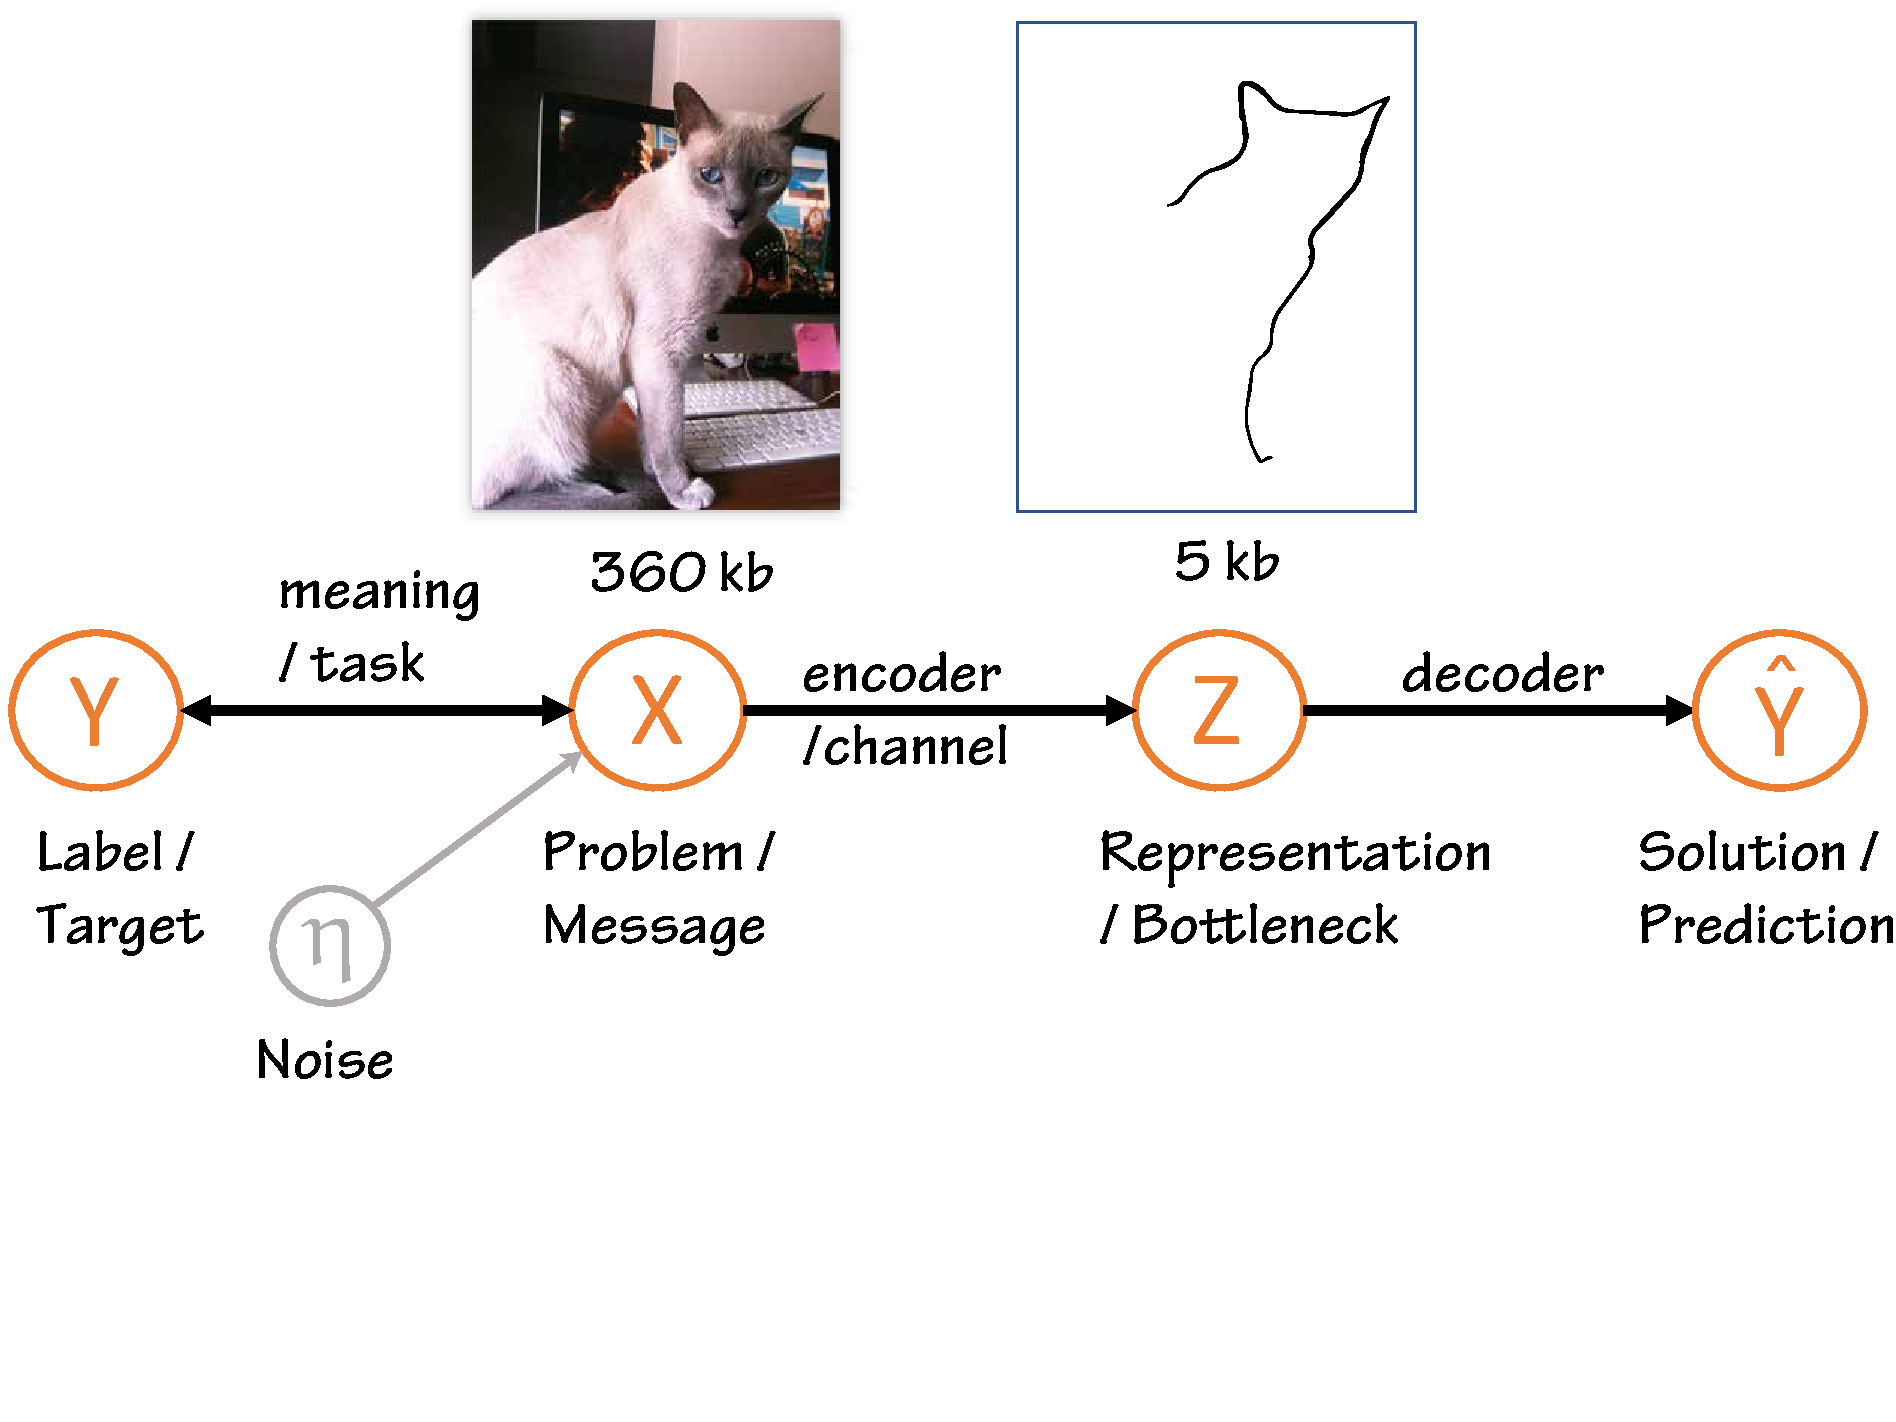
\includegraphics[width=1\linewidth]{ibt_learning_problem}
         \caption{The \ac{IBT} Learning Problem is the adaptation of the IB Problem to the learning setting.}
         \label{fig:ibt_learning_problem}
      \end{figure}

    \subsection{Definitions}
    \begin{enumerate}
      \item Let $\rvX$ be the random variable that denotes the
       \textbf{generator} (or \textbf{source}) of instance vectors $\rx$ of the learning problem  (\textbf{messages}), randomly draw from a probability distribution \(P(\rvX)\),\\ \(x\sim P(\rvX),~ x \in \sA_{\rvX} \);
       \item Let $\rvY$ be a random \textbf{relevant variable}  (the \textbf{Target}) which represents the solution $\ry$ for the problem $\rx$,~\ie the intended meaning $p(y|x)$ of the message $x$,\\
       \(y\sim P(\rvY),~ y \in \sA_{\rvY} \);
      \item A \textbf{task supervisor} knows the \textbf{task} distribution $P(\rvY|\rvX)$ and returns an output vector \(\ry_i\) for every input vector \(\rx_i\):\\
      $y_i := p(y|x_i)$;
      \item Let $\rvZ$ be a \textbf{bottleneck} random variable that denotes a compressed representation of the input $\rvX$ that is sufficient w.r.t. $\rvY$ and obeys the Markov chain $\rvY \leftrightarrow \rvX \leftrightarrow \rvZ$;
      \item Let the stochastic conditional distribution $q(z|x)$ be an \textbf{encoder}\footnote{A lossy encoder can be seen as a noisy channel.}of input instances into representations,\\
      $\rz := q(z|x)$.
      \item Let the stochastic conditional distribution $q(y|z)$ be a \textbf{decoder} of representations into solutions of the problem,\\
      $\hat{\ry} := q(y|z)$.
      \item A \textbf{learning algorithm} \(\AA\) which is the functional that given a dataset \(D_n = \{(\rx_1,\ry_1), \cdots, (\rx_n, \ry_n)\}\) of $n$ inputs and outputs of the task, selects a hypothesis \(h = \underset{\text{decoder}}{q(y|z)} \circ \underset{\text{encoder}}{q(z|x)} \) from the hypothesis space \(\HH\):
      \begin{align}
        \AA: \underbrace{(\XX \times \YY)^n}_{D_n} \to \HH .
      \end{align}
    \end{enumerate}

  \subsection{Assumptions}\label{sec:ibt_learning_assumptions}
  \begin{enumerate}
    [i.]
    \item The random variables $\rvX$, $\rvY$ and $\rvZ$ are \textbf{discrete};
    \item $\rvY \to \rvX \to \rvZ$ form a Markov-chain;
    \item $\sA_{\rvX}$, $\sA_{\rvY}$ and $\sA_{\rvZ}$ are \textbf{finite sets};
    \item \textbf{No assumption on \(\DD=\PXY\)}.
    \item \textbf{\(\DD=\PXY\) is unknown at the training stage}.
    \item \textbf{\(\DD=\PXY\) is fixed:} the ordering of examples in the sample is irrelevant.
    \item The generator/source $\rvX$ is an ergodic process (see \cref{ib_problem_setting}), therefore $x \sim p(x)$ are not necessarily mutually independent\footnote{This assumption is less constrained than independent sampling}.
		\item The encoder and the decoder are \textbf{stochastic} mappings \footnote{Notice that given the Markov chain $\rvY \leftrightarrow \rvX \leftrightarrow \rvZ$, due to reparemetrization invariance (Theorem \ref{th:reparemetrisation_invariance}), a deterministic mapping of the data does not throw out information, i.e. \ let $f:\aXX \to \aYY$ be deterministic, $I[f(\rvX);\rvY]=\IXY$.}.
		\item the \textbf{distortion measure} between $\rvX$ and its representation $\rvZ$ is $\IXY - \IZY = \KL(p(y|x)||p(y|z))$\footnote{This assumption is not strictly required, as it can be derived. The only reason to keep it here is to make the comparison of different problem settings easier.}.
  \end{enumerate}
\subsection{Problem statement}
Given the problem setting above, the \ac{IBT} learning problem is to find the encoder $p(z|x)$ and decoder $p(y|z)$ such that:
\begin{enumerate}
  \item the encoder maximises the compression of the input $\rvX$ into the representation $\rvZ$ while preserving the maximum information about the ``meaning'' $\rvY$. In other words, the encoder that generates minimal sufficient disentangled representations of the input.
  \item the decoder is trivial, as a result of the characteristics of the representation.
  \item The selection is based on a training set of $n$ i.i.d. observations drawn from an ergodic process $\PXY$.
\end{enumerate}
\subsection{Comparing IBT with other problems}
\subsection{IBT learning as a variational problem}
    Finding the encoder for minimal sufficient disentangled representations is equivalent to finding a distribution $p(z|x)$ that solves the following constrained optimisation problem.
    \begin{align}
        q(z|x):=\underset{p(z|x)}{\argmin} \quad  & \IZX  \\
        \textrm{s.t.}\quad
        & 0 \leq \IXY - \IZY \nonumber\\
        \quad & 0 \leq TC(Z)\nonumber
    \end{align}
    This non-linearly constrained optimisation problem\footnote{Prior to the publishing of \citeonly{alemi:2016} in 2017, there was no known algorithm to minimise the IB Lagrangian for discrete $\rvX$ and $\rvY$ with large state spaces or non Gaussian continuous joint distribution.} is very similar to the IB Problem (\cref{sec:IB_principle}). It just adds the total correlation constraint and assumes no knowledge over $\PXY$. ~\citeauthor{tishby:1999}~\cite{tishby:1999} proposed solving the IB problem using a relaxed minimization, the IB Lagrangian:
    \begin{equation}
        \begin{split}
        \underset{p(z|x)}{\min} \quad  & \IZX  \\
        \textrm{s.t.}\quad & \IZY \leq \IXY \\
        \end{split}
        \quad \Longrightarrow \quad
        \begin{split}
            &\min \IZX + \beta (\cancel{\IXY} - \IZY),\\
            &\min \IZX - \beta \IZY.
        \end{split}
    \end{equation}

    Let us also apply a Lagrangian relaxation to our representation learning problem:
    \begin{align}
        \LH &=  \IZX + \beta (\IXY - \IZY) + \gamma TC(z),\\
        \text{Let }\beta'&= \frac{1}{\beta}, \gamma'= \frac{\gamma}{\beta}\\
        \LH &=  \cancelto{\scriptscriptstyle \HYZ}{(\IXY - \IZY)} + \beta' \IZX + \gamma' TC(z),\\
        \LH &=  \HYZ + \beta' \IZX + \gamma' TC(z).
    \end{align}
    Let us denote $q_\theta(z|x)$ (encoder) and $q_\theta(y|z)$ (decoder) the unknown conditional distributions we want to estimate\footnote{$q_\theta(y|x)=\sum q_\theta(z|x) q_\theta(y|z)\\q(y|x,\theta^*)=p(y|x)$
    }, parametrized by $\theta$.

    Rewriting the Lagrangian as a per sample loss function, we have:
    \begin{align}
        H[\rvY|\rvZ] & \approx \E_{(x,y) \sim p(x,y)}[\E_{z \sim q_{\theta}(z|x)} - \log q_{\theta}(y|z)] \\
        \IZX & = \E_{x \sim p(x)} \KL(q_{\theta}(z|x)||p(z))\\
        TC(z) &= \KL(p(z)||\textstyle \prod_j q(z_j))\\
        \hat{\LH} &= \frac{1}{n} \sum^{n} \E_{z \sim q_{\theta}(z|x_i)} - \log q_{\theta}(y_i|z) \nonumber\\
         &+ \beta' \KL(q_{\theta}(z|x_i)||p(z)) \nonumber\\
         &+ \gamma' \KL(p(z)||\textstyle \prod_j q_{\theta}(z_j)).
    \end{align}

    The second and third terms of the loss are intractable, as we need to know $p(z)$ to compute, which is an unknown of our problem.~\cite{achille:2018infodropout}, however, prove that if $\gamma'=\beta'$, \ie we assume a factorised unknown distribution, the Lagrangian can be solved.

    \begin{align}
    \hat{\LH} = &\underbrace{\frac{1}{n} \sum^{n} \E_{q_{\theta}(z|x_i)} - \log q_{\theta}(y_i|z)}_{\hat H(p, p_{\theta})}\nonumber\\
    &+ \beta' \KL (q_{\theta}(z|x_i)||q_{\theta}(z)),~
    q_\theta(z)=\prod_j q_{\theta}(z_j).
    \end{align}

    Where $\hat H(p, p_{\theta})$ is the cross-entropy, and the second term is a regulariser that penalises the transfer of information from $\rvX$ to $\rvZ$. In other words, the regulariser penalises complexity measured as $\IZX$. The usage of cross-entropy loss and this kind of regularisers is widespread in practice. \cite{achille:2019phd} gave theoretical ground for such choices\footnote{The reference constraint their findings to \acp{DNN} optimised with \ac{SGD}. We find the result more general than that.}.

    \begin{corollary}
    Any learning algorithm that\footnote{This insight allowed \citeonly{alemi:2016,achille:2018infodropout} independently develop basically the same algorithm for estimating mutual information for any distribution using \acp{DNN}.}:
     \begin{itemize}
         \item assumes a stochastic $p(y|x)$;
         \item uses the cross-entropy loss;
         \item and a regularisation term that penalises the amount of information of the input stored in the model,
     \end{itemize} is learning a minimal sufficient disentangled representation and, in fact, solving a special case of the IB problem.
\end{corollary}

\section{Two levels of representation}\label{sec:2_levels}
Some criticism on works in what we are calling \emph{Information Bottleneck Theory} derive from a lack of rigour in explaining some basics (see \cref{sec:criticism}).

In \cref{ch:mlt}, we were presented with the \emph{learning problem} setting:
\begin{figure}[ht] \centering
    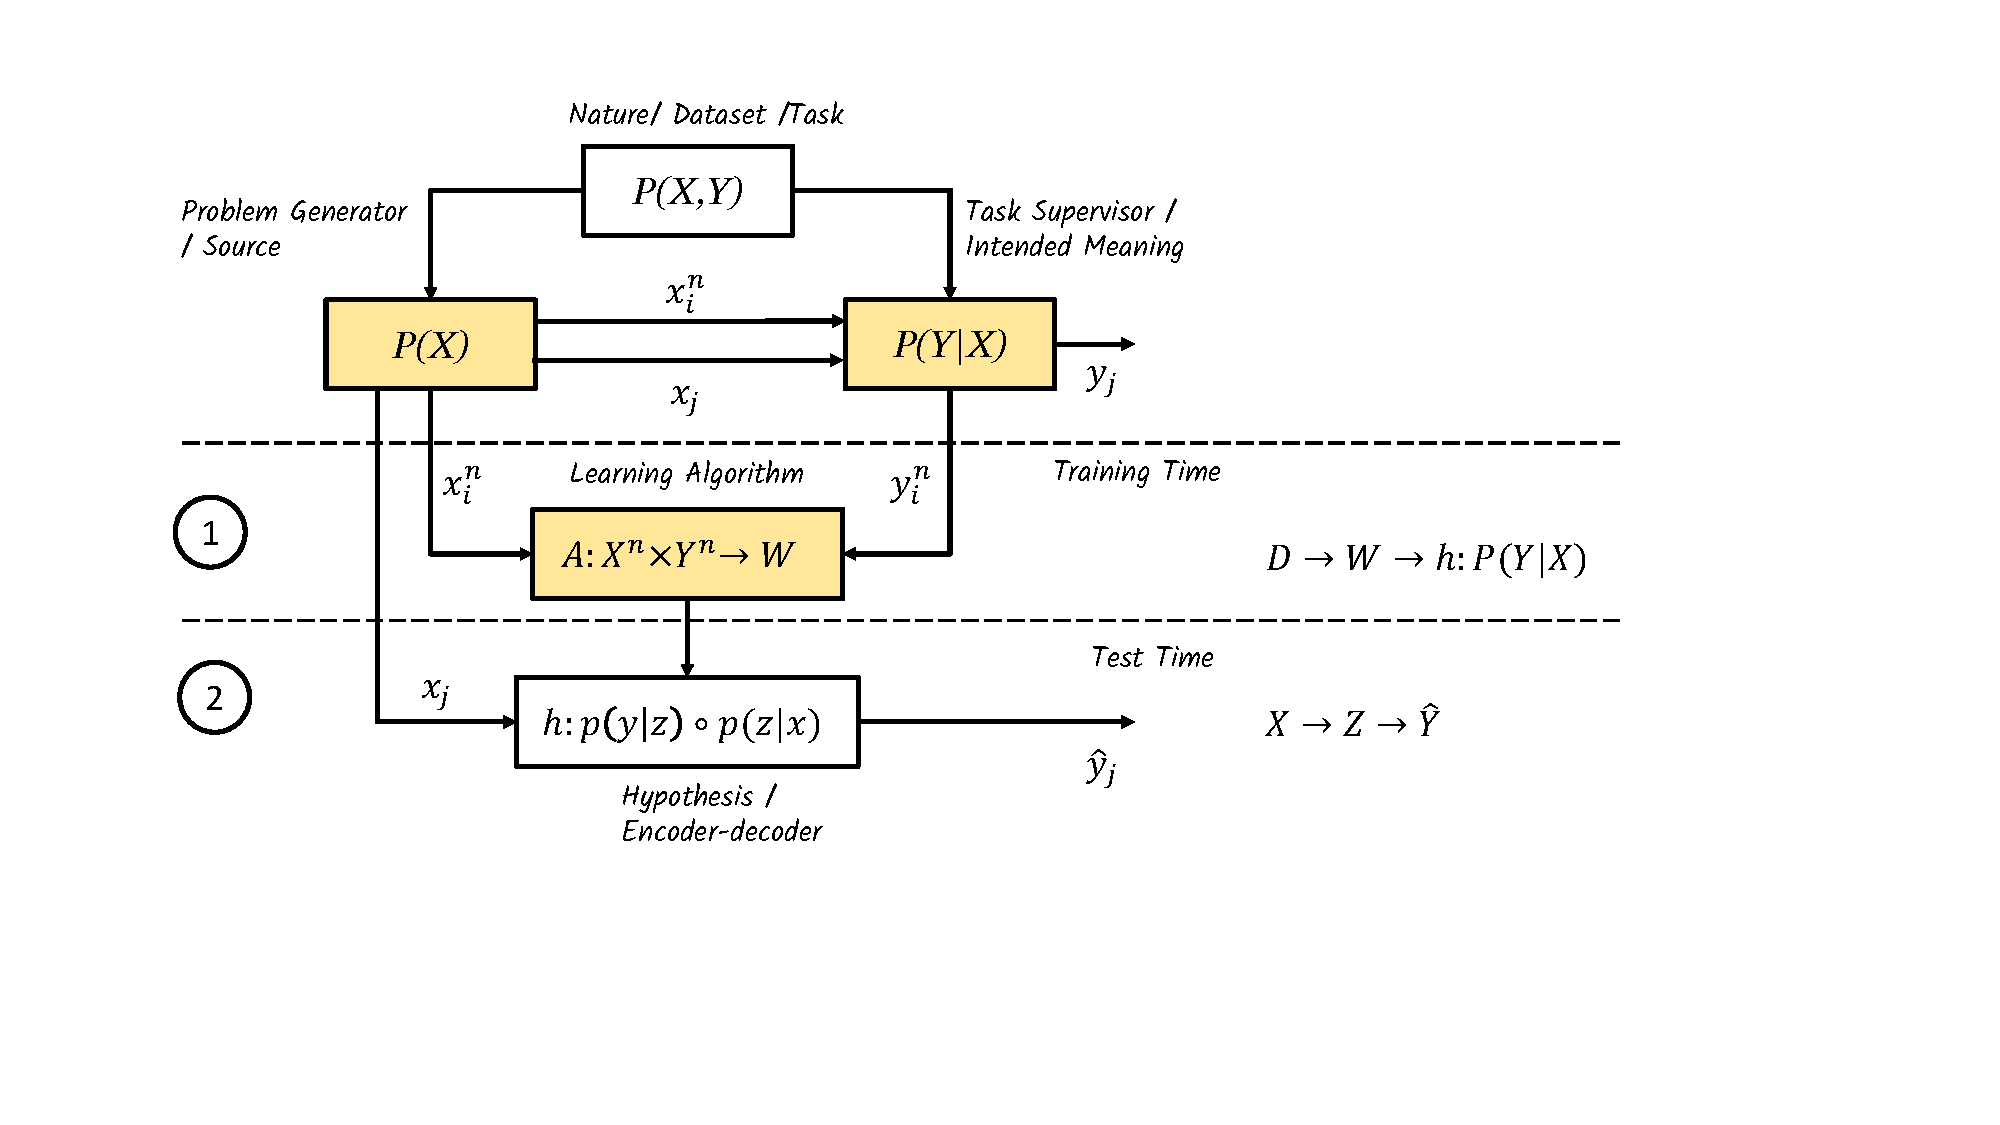
\includegraphics[width=
    \textwidth]{ibt_learning_setting}
    \caption{Two levels of representation in the learning setting.}\label{fig:two_levels_representation}
\end{figure}

The crucial problem in \ac*{MLT} is that we want to predict the behaviour (bound) of learning algorithms in future data while we can only access past performance. This dichotomy translates to representation learning by two intertwined but different representations:
\begin{enumerate}% [label=\protect\circled{\arabic*}]
  \item the representation of a \emph{dataset} (past data), a function that can be stored in memory for the later accomplishment of the task. It needs to keep useful information for future decisions without squandering resources in remembering spurious correlations or one-time events.
  \item the representation of an \emph{input example} (current data): which need to keep the essence of the scene at hand;
\end{enumerate}
% Why is this important? mTishby vs Achille

In~\cite{achille:2019phd, achille:2019weights}, borrowing the terminology of Deep Learning,~\citeauthor{achille:2019phd} call these two levels of representation of \emph{information in the weights} and \emph{information in the activations}, respectively.

Several \ac{IBT} papers to not address this difference. In special, some of the seminal work \cite{tishby:2015, shwartz-ziv:2017, tishby:2017}. How can we minimise the information in the activations, while we cannot access future data? There is a missing step.

We have to show how to bound future behaviour performance based only in the available training data.

Intuitively, there is a strong connection between  \emph{information in the weights} and \emph{information in the activations}. $\IZX$ which  measures the complexity of the activations representation, can be defined by the amount of weight in the network: low or zero weights will connect to the activations that are not in the optimal activation representation $z^*$ which minimizes $\IZX$.

In \cref{sec:duality}, we will formally address this issue.

\subsection[Rethinking generalisation: \\Cross-entropy and overfitting]{Rethinking generalisation: Cross-entropy and overfitting}
 In previous sections, we derived the use of the cross-entropy loss from a list of desired properties for representations(\cref{sec:desiderata})and that generalisation relates to the compressibility of the input(\cref{sec:invariant_if_minimal}). Still, what prevents the model to only memorise the map of training examples index to labels? Such memorisation seems a valid compression, need little information and will, obviously,not generalise.

 \cite{zhang:2016} demonstrates that the expressivity of \acp{DNN} is enough to fit random labels. Thus, at least for \acp{DNN}, generalisation is more \emph{not overfitting} than {not underfitting}.  This may be the case for other learning techniques as well. In this section, we will keep \emph{rethinking} generalisation on this new information-theorethic perspective and tray to elucidate how cross-entropy loss relates to overfitting and memorisation.

Classical \ac{MLT} assumes that we select an hypothesis $h$ parametrized by $\theta$. Conceptually, we already \emph{rethought} generalisation as being determined by the compressibility of the input (\cref{sec:invariant_if_minimal}). In this sense, the task is determined by the training dataset only\footnote{\citeonly{achille:2019phd} defines the task as the dataset distribution for which we only have one sample.}. Thus, we will assume the dataset is sampled from some generative model $P(\rvD|\theta)$. In this context~\cite{achille:2017emergence}:
\begin{theorem}
  Given $\rvD=(\rvX,\rvY),~ \rvD \sim P(\rvX, \rvY| \theta)$, and a representation $\rvW$ of $\theta$, s.t. $\rvY|\rvX \to W \to \theta$ form a Markov-chain:
  \begin{align*}
    H_{p,q}[\rvD|\rvW]=H_p[\rvD,\theta] + I[\theta;\rvD|\rvW] +
    \KL(p \parallel q)-I[\rvD;\rvW|\theta]
  \end{align*}
\end{theorem}
\begin{proof}
  First we will explain why minimizing $H_{p,q}[y|x]$ is equivalent to minimise $H_{p,q}[x,y]$
  \begin{align}
    H_{p,q}[y|x,w]=H_{p,q}[\rvD |\rvW].
  \end{align}
  When a learning algorithm optimises the cross-entropy loss, it is effectively just minimising the KL-divergence, as the first term (entropy) is a constant:
  \begin{align}
    H_{p,q}[y|x,w] = \cancel{H_{p}[y|x, w]} + \KL(p(y|x, \theta)||q(y|x, w)).  \tag{\text{from \eqref{eq:KL_decomposition}}}
  \end{align}
  The same happen in the inimisation of the cross-entropy of the joint dataset:
  \begin{align}
    H_{p,q}[x,y|w] = \cancel{H_{p}[x,y, w]} + \KL(p(x, y, \theta)||q(x, y, w))  \tag{\text{from \eqref{eq:KL_decomposition}}}
  \end{align}
   We still need to show that the divergence of $y|x$ is the same as the joint distribution $x,y$:
   \begin{align}
    &\KL(p(x,y) || q(x,y)) = \E_p \log \frac{p(x,y)}{q(x,y)}\\
    &= \E_p \log \frac{p(y|x)p(x)}{q(y|x)p(x)} = \E_p \left[\log p(y|x)p(x)- \log q(y|x)p(x)\right]\\
    &= \E_p \left[ \log p(y|x) + \cancel{\log p(x)} - \left( \log q(y|x) + \cancel{\log p(x)} \right) \right]\\
    &= \E_p \left[\log p(y|x) - \log q(y|x) \right]= \E_p \log \frac{p(y|x)}{q(y|x)}\\
    &= \KL(p(y|x)||q(y|x))
  \end{align}
  Therefore we can say that a learning algorithm minimises $H_{p,q}[\rvD|\rvW]$.
  \begin{align}
    H_{p,q}[\rvD|\rvW] = H_{p}[D, W] + \KL(P(\rvD, \theta) \parallel Q(\rvD, \rvW))  \tag{\text{from \eqref{eq:KL_decomposition}}}
  \end{align}
   To prove that:
   \begin{align*}
    H_{p,q}[\rvD|\rvW]=H_p[\rvD|\theta] + I[\theta;\rvD|\rvW] +
    \E\KL(p \parallel q)-I[\rvD;\rvW|\theta],
   \end{align*} we just need to prove that:
   \begin{align}
    H_p[\rvD|\rvW] = H_{p}[\rvD, \theta] + I[\rvD|\rvW; \theta] - I[\rvD; \rvW|\theta].
  \end{align}
  Which is clear with the help of the following Venn diagrams\footnote{Our assumptions guarantee that all information measures in the diagram are positive, thus there is no problem in using the Venn diagram in this case.}:
  \begin{align*}
    &\vcenter{\hbox{\begin{venndiagram3sets}[shade=blue!30!white,labelA={$\rvD$},labelB={$\rvW$}, labelC={$\theta$}, tikzoptions={scale=.4}]]
          \fillANotB
        \end{venndiagram3sets}}}  &\ =\
    \vcenter{\hbox{\begin{venndiagram3sets}[shade=blue!30!white,labelA={$\rvD$},labelB={$\rvW$}, labelC={$\theta$}, tikzoptions={scale=.4}]]
          \fillANotC
        \end{venndiagram3sets}}}  &\ +\
    \vcenter{\hbox{\begin{venndiagram3sets}[shade=blue!30!white,labelA={$\rvD$},labelB={$\rvW$}, labelC={$\theta$}, tikzoptions={scale=.4}]]
          \fillACapCNotB
        \end{venndiagram3sets}}}  &\ -\
    \vcenter{\hbox{\begin{venndiagram3sets}[shade=blue!30!white,labelA={$\rvD$},labelB={$\rvW$}, labelC={$\theta$}, tikzoptions={scale=.4}]]
          \fillACapBNotC
        \end{venndiagram3sets}}} \\
    &H_p[\rvD|\rvW]  &\ =\ H_p[\rvD|\theta]  &\ +\ I[\rvD|\rvW; \theta]  &\ -\ I[\rvD; \rvW|\theta]
  \end{align*}
\end{proof}
Let us examine the cross-entropy decomposition:
\begin{align*}
  H_{p,q}[\rvD|\rvW]=\underbrace{H_p[\rvD|\theta]}_{\text{intrinsic error}} + \underbrace{I[\theta;\rvD|\rvW]}_{\text{sufficiency}} +
  \underbrace{\KL(p \parallel q)}_{\text{efficiency}}-\underbrace{I[\rvD;\rvW|\theta]}_{\text{memorisation}}
\end{align*}
\begin{description}% [wide=0\parindent]
  \item[intinsic error:] $H_{p}[\rvD,\theta]$ relates to the intrinsic error that we would find even if we knew $p_{\theta}$;
  \item[sufficiency:] $I[\theta;\rvD|\rvW]$ measures how much information of $\theta$ was compressed in the weights;
  \item[efficiency:] $\KL(p \parallel q)$ measures the efficiency of the representation,\ie the number of additional bits we need to represent the input with $q(w|D)$ instead of using $p_{\theta}$ (see \cref{sec:cross-entropy});
  \item[memorisation:] $I[\rvD;\rvW|\theta]$ is the last and only negative term. It relates to overfitting and measures how much information about the dataset is memorised in the weights.
\end{description}
Being the only negative term, the optimiser will try to increase memorisation. \cite{achille:2017emergence} proposes a naïve method to eliminate this proness to overfitting: adding back the memorisation term in the loss.
  \begin{equation}
    \LL(\rvW) = H_{p,q}[\rvD|\rvW] + I[\rvD;\rvW|\theta]
  \end{equation}
To calculate $I[\rvD;\rvW|\theta]$ true distribution, $p_\theta$ is needed. But wejust trying to approximate $p_\theta$ with $q$ during training. Hence we are presented with \emph{chicken-egg} problem. Rather, one can add a Lagrangian multiplier to upper bound $I[\rvD;\rvW|\theta]$:
  \begin{equation}
    \LL(\rvW) = H_{p,q}[\rvD|\rvW] + \underbrace{\beta I[\rvD;\rvW] }_{\text{Information in the Weights}}  \label{eq:new_IBL}
  \end{equation}
Remarkably, this has the same form of the IB Lagrangian equation (\cref{IB_Lagrangian}). When $\beta=1$, \eqref{eq:new_IBL} reduces to the ELBO loss used in variational inference\cite[p. 53]{achille:2019phd}.

\subsection{A new Information Lagrangian}
The question now is if this new Lagrangian emerged from trying to eliminate overfitting is somehow related to the IB Lagrangian in the activations presented before.
\begin{align*}
  \underset{\text{input}}{\rvX} \xrightarrow{\hspace*{1.4cm}}\underset{\text{activations}}{\rvZ}& \xrightarrow{\hspace*{1.4cm}}\underset{\text{label}}{\rvY}\\
  \underset{q(\rvZ|\rvX)}{\min\LL(W)} = H_{p,q}[\rvY|\rvT]& + \IZX \tag{Activations IB}\\
  \underset{\text{dataset}}{D} \xrightarrow{\hspace*{1.4cm}}\underset{\hspace*{.15cm}\text{weights}\hspace*{.15cm}}{W}& \xrightarrow{\hspace*{1.4cm}}\underset{\text{real distribution}}{P(\rvY|\rvX)\hspace*{.5cm}}\\
  \underset{q(\rvD|\rvW)}{\min\LL(W)} = H_{p,q}[\rvD|\rvW]& + \IDW \tag{Weights IB}\\
\end{align*}

\cite[Corollary C.8]{achille:2017emergence} have proved that indeed $\IZX \leq \IWD$. As $\IWD$ can be calculated, this development allows one to explicitly regularize the training.  That is exactly what \cite[Information Dropout]{achille:2018dropout} proposes.

\section{Connection to VAE}
\section{Connection to PAC-Bayes}
\section{Connection to MDL}
\section{Evidence of the IB limit in a human learned task}\label{sec:efficient_color_naming}

    \citeauthor{zaslavsky:2018}~\cite{zaslavsky:2018} had the sagacious idea of using the IB method to analyse anthropological evidence.

    We have already established that intelligent agents, whether artificial or biological, need language to represent a complex environment. Natural languages reflect different solutions to this problem. The current most accepted theory in Anthropology and Linguistics suggest that while languages vary to accommodate language-specific needs (due, for example, to variations in the environment), they evolve into efficient representations~\cite{zaslavsky:2018}. Although not explicit in~\cite{zaslavsky:2018}, it is evident that the evolution of natural languages can be seen as a learning process for the task of efficient communication by a society.

    The paper analyses natural languages in the context of colour naming. It is based on the World colour Survey (WCS), \emph{a large colour-naming database obtained from informants of mostly unwritten languages spoken in pre industrialised cultures that have had limited contact with modern, industrialised society}~\cite{lindsey:2009}. Assuming that each colour of WCS corresponds to a specific meaning, it  formulates the problem of colour naming in an information-theoretic perspective analogous to the IB problem setting~\cite{tishby:1999}:

    \begin{figure}[ht!]
        \centering
        \begin{align*}
            \begin{array}{ccccccc}
                \tiny \text{Target} & \tiny \text{Intended Meaning} &\tiny \text{Source} &\tiny \text{Encoder} & \tiny \text{Representation}&\tiny \text{Decoder}  &\tiny \text{Estimated Target}\hspace{\fill} \\
                    \\
                \rvY &\underset{p(y|x)}{\longrightarrow} &\rvX &\underset{q(z|x)}{\longrightarrow}&\rvZ&\underset{q(y|z)}{\longrightarrow}  &\hat{\rvY} \\ \\
                \rvU &\underset{m(u)}{\longrightarrow} &\rvM &\underset{q(w|m)}{\longrightarrow}&\rvW&\underset{\hat{m}_w(u)}{\longrightarrow}  &\hat{\rvM} \\ \\
                \tiny \underset{ \text{\tiny(colour)}}{\text{Universe}} & \tiny \text{Intention} &\tiny \text{Source} &\tiny \underset{\text{\tiny (naming distribution)}}{\text{Language}}&\tiny \text{Word}&\tiny \text{Language}  &\tiny \text{Interpretation}
            \end{array}
        \end{align*}
    \end{figure}

    With that formulation, it is possible to calculate the IB limits and analyse the different languages colour-naming solutions in this framework:
    \begin{figure}[hbt!]
        \centering
        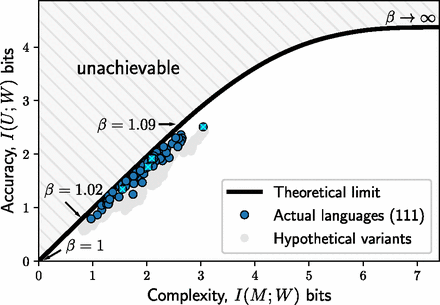
\includegraphics[width=0.7\linewidth]{efficient_colornaming_result}
        \caption{Different languages (blue circles) achieve near-optimal compression (IB curve in black)~\citeonly{zaslavsky:2018}. Reproduced with permission.}\label{efficient_colornaming_result}
    \end{figure}

    In \cref{efficient_colornaming_result}, it is possible to see evidence that languages efficiently compress ideas into words by optimising the tradeoff between complexity and accuracy of the lexicon according to the IB principle.

    This analysis corroborates the current theory on human language evolution. The drive for information-theoretic efficiency explains why human languages categorise colour as they do and may also apply to learning in general.

    Assuming the hypothesis, languages evolve to become more efficient in a tradeoff between conciseness (complexity, generalisation) and precision. The prediction capability is just an expected consequence of an efficient representation of meaning. The conciseness of the representation of knowledge, given an acceptable error margin, is a proxy of the agent's intelligence. The IB limit is an epistemic limit that is valid for machines, humans and aliens.

\section{Concluding Remarks}

<<<<<<< HEAD
- Cronologia X Didática
- Assumptions minhas. Finite
- Quantização
=======

>>>>>>> 1423702bbc26153edcfd7a58dee083e0fcfdf6ad



% \section{IB Learning}
% \subsection{The IB Lagrangian}

% \begin{itemize}
% 	\item IB solution assumes $P(X,Y)$ is given
% 	\item if unknown, MI intractable
% 	\item use proxies instead
% 	\item analitically solvable for distributions in the exponential family
% 	\item soft generalisation of minimal sufficiency
% \end{itemize}

% a task is a set of decisions to be taken given observed data;
% • a representation of a task is a function of data that can be computed and stored in memory for later acomplishment of the task.
% • an optimal representation is one that enables the best task performance given available data and resources.
% We need to differentiate 2 interwined but different representations in this discussion:
% 1. the representation of the training set (past data), stored in the weights of the network; 2. the representation of current input, encoded in the activations of the network;
% Each attend different tradeoffs (optimisation criteria):
% 1. weights need to store useful information for future decisions, without squandering resources in remembering spurious correlations or one-time events;
% 2. activations need to represent essential details of the scene at hand, without squandering resources in useless details;
% • Thedichotomyabovecreatesafundamentalproblem:desirablepropertiesoftheactivationsconcern representation of future data, while we only have past data to optimise a representation.
% • Information of what, for what, relative to what: Data reduces uncertainty in the task. The amount of uncertainty reduction is the information the data contains about the task. Reasoning about infor- mation requires specifying information of what (the data), for what (the task), relative to whatever prior uncertainty was present before the data was available.

% (Informationintheweights)Theyarguethatgivenasourcedata,andastochastictrainingalgorithm, the output weight w of the training process is a random variable (that depends on the stochasticity of the initialisation, training steps, and the data); i.e. w is a representation of the dataset D and we can talk about I(w;D). Instead of computing or optimising I(w;D), they want to control it by injecting noise in the weights that can be modulated between zero to an amount large enough that no information is left.
% 

%************************************************
\chapter{The Information Bottleneck and Deep Learning}\label{ch:ib_and_dl}

%************************************************
\begin{quotation}
	\small \textit{ \flushright
	Great claims require great evidence.
	\flushright --- Carl Sagan \\
	\vspace{1cm}}
\end{quotation}


This chapter presents:
% - ### IB and Deep Learning
% 	- #### Types of works on IB in DL (Intro)
% 		- ##### DNN analysis/criticism
% 		- ##### Applications
% 			- IB based algorithms
% 			- Transfer Learning
% 		- ##### IB theory of DL
% 	- #### DNN analysis/criticism
% 		- IB as X-ray
% 		- Saxe et al.
% 		- Goldferb et al.
% 		- Deep Invertible networks
% 		- M.I. measurement
% 		- Invertible Deterministic function: $H(T)=H(X)$
% 		- "It is a known fact that the IB is ill-posed for deterministic (...)", Tishby video
% 		- stochastic function?
% 		- Quantization, computers
% 		- Dataset has some stochasticity
% 	- #### IB based training and algorithms (applications)
% 		-   Achille, Soatto
% 		-   Alemi, Fischer
% 	- #### IB theory of DL
% 		- comparing assumptions
% 		- Shamir, Sabato, Tishby
% 		- Achille, Soatto
% 		- ##### new narrative for explainable phenomena
% 			- ###### flat minima
% 				- Hochreit and Schimdhuber
% 				- MacKay Evidence Framework
% 				- Achille Implicit regularization (Fischer information)
% 			- ###### the role of layers in DL
% 				- Achille misses the point
% 				- original explanation based on IBT
% 		- ##### new explanations for unexplainable phenomena
% 			- ###### Critical Learning Periods
% 			- ###### Super convergence
% 				- (GAP) Research opportunity for original contribution
% 		- ##### Activations vs weights
% 			- ###### duality
% 				- different meanings
% 				- $\min I(D;W) \to \min I(X;T)$, proof by Achille
% 		- ##### Information in the Activations
% 			- ###### deterministic
% 			- ###### In videos, Tishby clearly understand the duality of activation and weights
% 			- ###### Tishby's work mixed analysis with explanations.
% 			- ###### Critics didn't like explanations (of information in the activations. Lack of rigor.) and discarded the analysis
% 		- ##### Information in the weights
% 			- ###### emergence of regularization term
% 				- SGD implicit regularization
% 			- ###### Connection to PAC-Bayes
% 				- vacuous PAC-bayes bounds
% 				- from PAC-Bayes to IB Lagrangian
% 				- Achille aims to show connection, not to suggest new bounds
% 		- ##### Sample bounds on empirical MI
% 			- Shamir, Sobato, Tishby
\section{Types of literature on Information Bottleneck and Deep Learning}
Critics point out that the output of some learning algorithms are invertible deterministic functions and, as such, due to reparametrisation invariance (Theorem \ref{th:reparemetrisation_invariance}), they do not change the amount of information of the input. In these cases, there is no compression, and the amount of information in the representation is equivalent to the input's entropy. Tishby argues that any learning algorithm has noise due to finite computer memory and are not deterministic. Besides, he proposes injecting noise in the running of every \emph{snapshot}, a kind of \emph{test time augmentation}\footnote{\bt{Test time augmentation} is a common practice in ML that injects noise to a test input, by generating transformed versions of it, and combines the predictions of these versions.}, to measure information, which will lead to slightly different $\hat{\ry}_i$  in different runs of the model for the same $\rx_i$.


Despite calling his work \emph{Information Bottleneck Theory}, Tishby admits it is not ``rigorously proven'' theory, and he argues that the initial strong criticism is ``throwing the baby with the water''. For him, the IB should be seen as a tool, an ``X-Ray'', to analyse the behaviour of learning algorithms during training\footnote{In reality, his focus has been on analysing Deep Learning models.  This argument, however, can be applied to any learning algorithm.}~\cite{tishby:2020DeepMath}. For this, he is interested in measuring information in the representation of {input examples} (\emph{information in the activations}) during training. Each sample fed to the training generates a ``snapshot'' of the quality of representations being generated.


\section{IB based analysis of Deep Learning}
In their numerical experiments\cite{shwartz-ziv:2017}, they use unregularized fully connected feed-forward neural networks with hyperbolic tangent hidden layer activation functions, SGD and cross-entropy loss function. To estimate $I[\rvX;\rvZ_L], I[\rvY;\rvZ_i]$, they bean each neuron's double-soded saturation arctan output activation into 30 equal intervals to calculate the mutual information pair over epochs. They produce the information plane over 50 different randomized initializations.  Visual appealing... 2 distinct phases. First, in a shorter empirical error minimization (ERM) phase and a much longer compression phase, $I[\rvX;\rvZ_L]$ gradually decreases. Learning is forgetting. authors suggest this representation compression phase is enabled by SGD's diffusion-like behavior and responsible fort the generalisation performance.
\subsection{Tishby's main thesis}
Learning is forgetting
Information Plane
\subsection{Criticism to Tishby's main thesis}\label{sec:criticsm}
\citeauthor{shwartz-ziv:2017} results were challenged shortly after by \cite{saxe:2018}. Foremost, \citeauthor{saxe:2018} note that the use of a binning procedure to estimate mutual information is ambiguous, as the true mutual information between $I[\rvX;\rvZ_L]$ is provably infinite for continuous distributions and constant (\ie equal to $H[\rvX])$ for discrete distributions. Reparemetrisation property -> and activation function is invertible transformation (deterministic mapping) of input. The binning injects noise that is external to the network. They replicated the experiment with an identical tanh-actication, but also tried alternative versions with ReLU, softsign and softmax. The ReLU function do not comproess in their experiment. They also take into account that the plotted mutual information results are incluenced by the user-selected nmber of bins and binning strategy. Overall, \citeauthor{saxe:2018} refute \citeauthor{shwartz-ziv:2017} results.
\cite{goldfeld:2019} show that their $I[\rvX;\rvZ_L]$ estimates does not directly measure compression of the true mutual information.
\cite{chelombiev:2018} explore several estimation schemes for measuring compression and propose an entropy-based adaptative binning strategy (EBAB). Under EBAB, the RELU exhibits much more compression. They make the caveat regarding how initialization may affect information plane.
\citeauthor{achille:2017emergence} take a related but different approach. They create their own IB Lagrangian between weights and data. They relate their Lagrangian to PAC-Bayes framework. They propose that information in weights is not only a measure of learned model complexity, but also relates to a transition from underfitting to overfitting.They show that DNNs are not inconsitent with bias-variance trade-off theorem if complexity is interpreted in terms of information rather than dimensionlity. They demonstrate this deriving a cross-entropy loss decompposition.
Hp.q = intrinsic error + sufficiency + efficiency + overfitting

The implicit overfitting term in cross-entropy suggest one can overcome overfitting by adding back the overfitting term.

They also empirically validate 3 main takeawyas: there is a transition from overfitting to underfitting, the bias-variance trade-off holds when interpreted in terms of information and that by decreasing information in the weights representations can be made insensitive to nuances.
.... empirical ....
Achille and Soatto produce a generally satisfying theoretical work.

information-plane visually appealing contribute dto the popularity.. lack theoretical rigor.

Achille and Soatto research, in contraposition, is trying to use the IB framework not only to explain but also to improve learning algorithms.  In their view, noise during training helps generalisation. They argue that the noise in Stochastic Gradient Descent is responsible for Deep Learning generalisation power. Moreover, they believe that generalisation can be further improved by controlled injection of noise during training. They are interested in measuring and \emph{controling} the information in the representation of the task (\emph{information in the weigths}).
- IB as X-ray
		- Saxe et al.
		- Goldferb et al.
		- Deep Invertible networks
		- M.I. measurement
		- Invertible Deterministic function: $H(T)=H(X)$ information is a property of random variables, which may be degenerate for the deterministic pro- cess of computing the output of a trained DNN in response to a given input (inference). Achille and Soatto 2021

		- "It is a known fact that the IB is ill-posed for deterministic (...)", Tishby video
		- stochastic function?
		- Quantization, computers
		- Dataset has some stochasticity
		subsubsection This is a weakness

		- quantization: Because quantization is a many-to-few mapping, it is an inherently non-linear and irreversible process (i.e., because the same output value is shared by multiple input values, it is impossible, in general, to recover the exact input value when given only the output value).
		Assuming neural networks are non-linear non-inversible functions, finite hypothesis space
		The set of possible input values may be infinitely large, and may possibly be continuous and therefore uncountable (such as the set of all real numbers, or all real numbers within some limited range). The set of possible output values may be finite or countably infinite.[6] The input and output sets involved in quantization can be defined in a rather general way. For example, vector quantization is the application of quantization to multi-dimensional (vector-valued) input data. In the typical case, the original signal is much larger than one least significant bit (LSB). When this is the case, the quantization error is not significantly correlated with the signal, and has an approximately uniform distribution.
		- Turing \cite{turing:1936} countable set of all possible computer programs -> set of computable real numbers is also countable -> The set of reals in uncountable -> most reals are uncomputable, infinitely many more than are computable. Algebraic reals can be computed digit by digit.
		- no physical quantity has ever been measured with more than twenty digits of precision\cite[p. 92]{chaitin:2006}
		- philosophical and mathematical argument against the physical existance of real numbers \cite[99-116]{chaitin:2006}
\subsection{The faux plane}
	Experimental results that corroborate to
\section{IB based training and algorithms}
Achille
Alemi, Fischer
\section{IB Theory of Deep Learning}
\subsection{A new narrative for understanding Deep Learning Phenomena}


% \subsection{Possible explanations for unexplained Deep Learning Phenomena}
% Several pleasant features underlay the success of deep learning: The scarcity of bad minima en- countered in their optimization [Draxler et al. (2018); Choromanska et al. (2014)], their ability to generalize well despite being heavily over-parametrized [Neyshabur et al. (2018, 2014)] and expres- sive [Zhang et al. (2016)], and their ability to generate internal representations which generalize across different domains and tasks [Yosinski et al. (2014); Sermanet et al. (2013)]. Our current understanding of these features is however largely empirical.Internal representation are a key ingredient in transfer learning [Yosinski et al. (2014); Sermanet et al. (2013)]
\subsection{Generalization power despite number of parameters}
\subsection{Generalization despite expressiveness--overfitting}
\subsection{ability to generate internal representations which generalise across domains and taks}
\subsection{Scarcity of bad minima encountered in their optimisation}
\begin{figure}[h]
  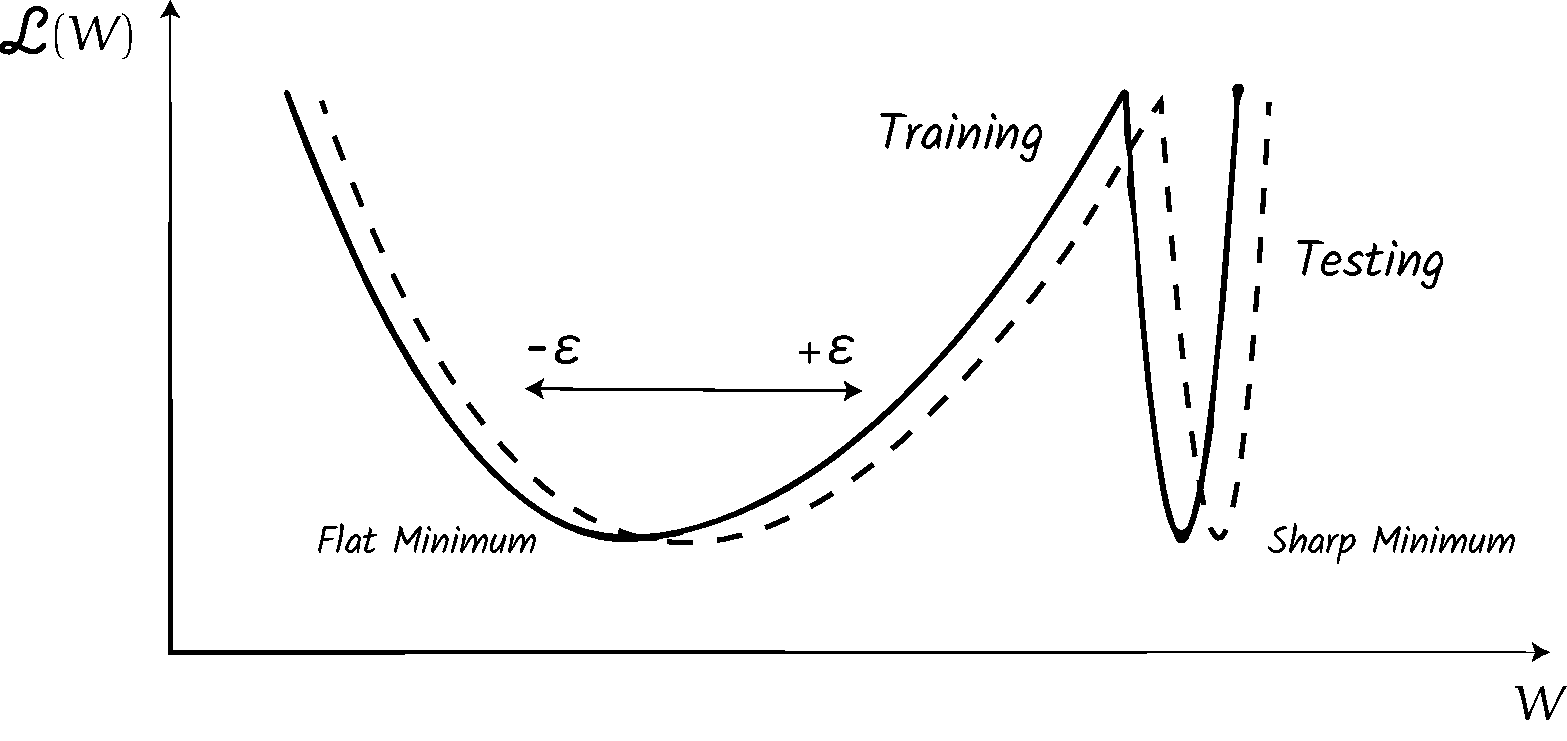
\includegraphics[width=\columnwidth]{flat-minima}
  \caption{Information in the weights explain the preference of SGD for flat minima.}
  \label{fig:flat_minima}
\end{figure}
The relation of low Fisher Information in the weights and good generalization in the activations bring us another interesting insight. It is a well documented phenomena that DNNs trained with SGD tend to find flat minima, meaning saddle points where some noise in the test data will minimally affect the loss (see figure \ref{fig:flat_minima}).  Here we have a theoretical reason why this is happening. SGD is implicitly regularizing the information in the weights and that is the same as looking for minimas with low Fisher Information, which are Flat Minimas.

Hochreiter and Schmidhuber discuss sharp versus flat minima using the language of minimum de- scription length In short, describ- ing weights in sharp minima requires high precision in order to not incur nontrivial excess error, whereas flat min- imum can be described with lower precision. A similar coding argument appears in [HC93].

\subsection{The role of layers in deep learning}
Why do we need multiple layers in a neural network? This question is fundamental in Deep Learning, and still, there is no definitive answer. A feedforward network with a single layer can represent any function\cite{goodfellow:2016}. Also, \cite{leshno:1993} (as cited by \cite{goodfellow:2016}) demonstrated that shallow networks with rectified linear units as activation functions have universal approximation properties. When confronted with these facts, the usual answer for the need for depth is that these results require an infeasible large layer or do not address efficiency. Another common answer is that layers provide levels of abstraction and a paramount composability property, \ie stacking layers allow a network to represent functions of increasing complexity\cite{goodfellow}. These answers seem correct but, at the same time, somewhat qualitative and vague\footnote{Teo: Any reference of quantitative proof for the need for depth?}.

This section will try to advance the discussion by answering the need for depth in Neural Networks with an Information Bottleneck perspective.

We have already established that a DNN optimised with SGD solves an \ac{IB} problem. In this view, the body of the network is an encoder that compresses the input $\rvX$ into a representation $\rvZ$. In the IBT perspective, training  a DNN is finding the encoder that minimises $\IZX$:
\begin{align*}
	Q(\rvZ|\rvX)~|~Q = arg\ min\ \IZX
\end{align*}

From~\cite{achille:2017emergence}:
\begin{corollary}[Bottlenecks promote invariance] Assume a Markov chain of layers:
	\begin{align*}
		\rvX \to \rvZ_1 \to \rvZ_2,
	\end{align*}
and that there is a bottleneck between $\rvZ_1$ and $\rvZ_2$ (for example, if $dim(\rvZ_1)>dim(\rvZ_2)$ or noise has been added between to the channel $\rvZ_1 \to \rvZ_2$ via dropout\footnote{Dimensionality reduction can be seen as a form of noise.}). Then, if $\rvZ_2$ is sufficient, it is more invariant to nuisances than $\rvZ_1$ (see \cref{sec:invariant_if_minimal}).
\end{corollary}

\begin{corollary}[Stacking increases invariance] Assume a Markov chain of layers:
	\begin{align*}
		\rvX \to \rvZ_1 \to \rvZ_2 \to \cdots \to \rvZ_L,
	\end{align*}\label{cor:stacking_layers}
	and that $\rvZ_L$ is sufficient of $\rvX$ w.r.t. $\rvY$. Then, by \ac{DPI}:
	\begin{align*}
		I[\rvZ_L;\rvX] \leq I[\rvZ_i;\rvX], \forall i \in \{1 \cdots L-1\},
	\end{align*}
	therefore $\rvZ_L$ is more insensitive to nuisances than all preceding layers and generalises better.
\end{corollary}

In other words, \citeauthor{achille:2017emergence} argue  that \textbf{stacking layers improve generalisation}.
A problem with this argument is that It only shows that in the multi-layered scenario, the last layer is more compressed and invariant to nuisances. It is not direct that a single-layered network can not achieve the same level of compressibility of the input as the last layer in the multi-layered scenario.

Besides, according to \cite{achille:2017emergence}, the above corollary does not simply imply that the more layers, the merrier, as it assumes that one has successfully trained the network ($\rvZ_L$ is sufficient). For the authors, a successfully trained network becomes increasingly difficult as the network grows.The increase in difficulty seems straightforward because stacking layers increase the number of computations per batch.

By pure logic, it is evident that the complexity of any algorithm that searches for the best possible hypothesis will depend on the size of the hypothesis space. Counterintuitively, however, we claim that \bt{stacking layers decrease the complexity of the training in practice}, as they reduce the ``typical'' hypothesis space size. We argue that stacking layers increase the complexity of the learning algorithm by a constant while exponentially decreasing the size of the ``typical'' hypothesis space.

To explain how stacking layers reduce the ``typical'' hypothesis space size, let us start with the case of a single layer DNN. We need to find:
\begin{align}
	Q_1^* = Q_1(\rvZ_1|\rvX)~|~Q_1^* = arg\ min\ \IZX
\end{align}

What is the ``typical'' hypothesis space in this case? First, let $\sA_{\rvQ_1}$ be the hypothesis space of all functions that encode $\rx \in |\sA_{\rvX}|$ possible inputs into $\rz \in |\sA_{\rvZ}|$ possible outcomes. Nevertheless, from Shannon's Noisy Channel Theorem (\cref{noisy_channel_theorem}) there are only $2^{H[\rvX]}$ typical $\rx_i$ and for each typical $\rx_i$ there is only $2^{H[Z|X]}$ ``typical'' outcomes (see \cref{sec:source_encoding_theorem}), therefore, the number of decodable encodings (one to one mappings) is:
\begin{align}
\forall q \sim \sA_{Q_1},&~Pr(q \in \sA_{Q_1}^\epsilon) = 1 -\epsilon, \epsilon < \dfrac{1}{2}\\
|\sA_{Q_1}^\epsilon| &= \frac{2^{H[\rvX]}}{2^{H[\rvZ_1|\rvX]}}=2^{\IZX}.
\end{align}
where $\epsilon$ can be arbitrarily small.
\begin{figure}
	[ht!] \centering
	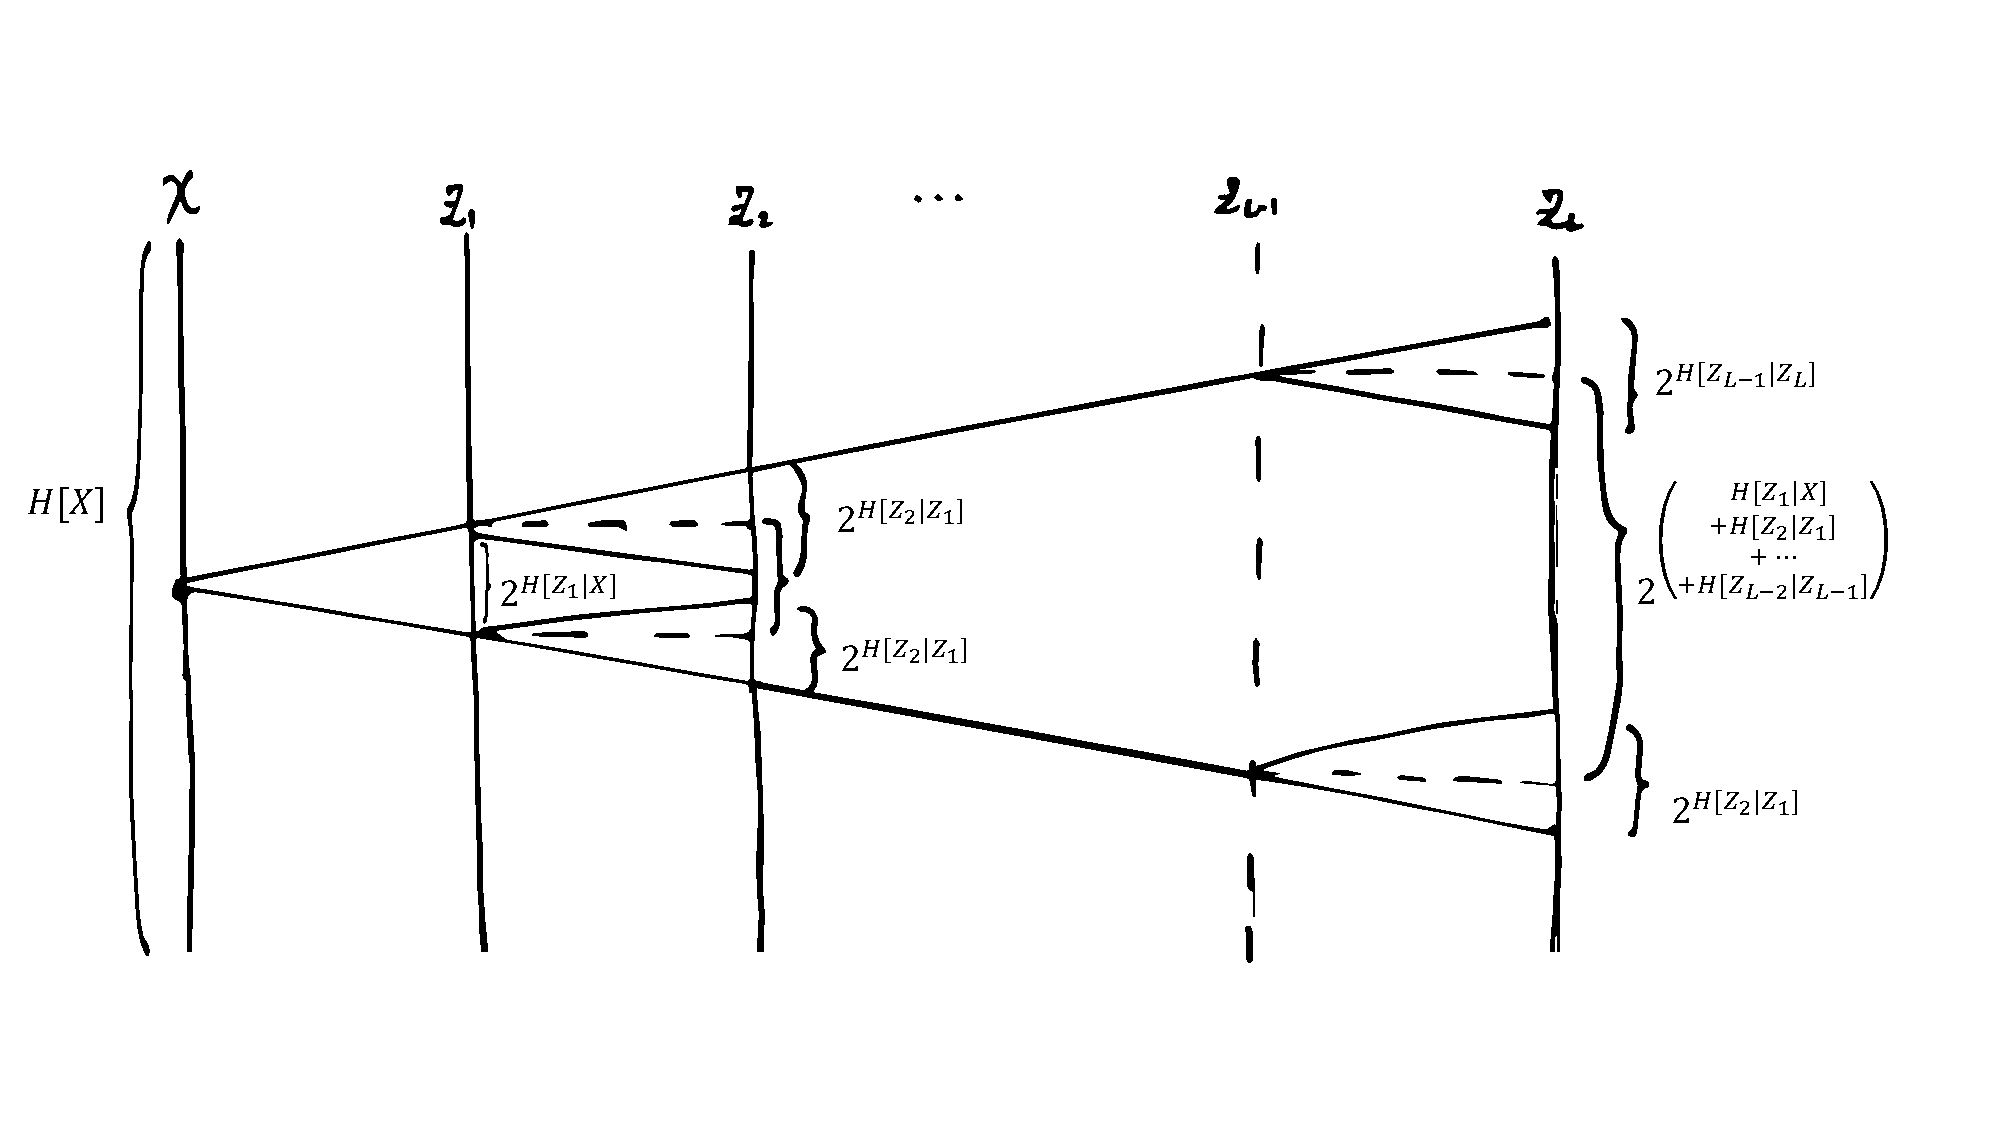
\includegraphics[width=\textwidth]{multi_layers}
	\caption{A visual explanation of corollary \ref{cor:stacking_layers}, stacking layers decrease the mutual information.}\label{fig:stacking_layers}
\end{figure}

Now, let us compare with the case of $L$ layers. Each layer acts as an encoder $q_i:\rvZ_{i-1} \to \rvZ_i$. The typical hypothesis space of $q_i$ depends on the cardinality of the possible values of $z_i$, which will depend on the size of the typical hypothesis space of $q_{i-1}$ (a one-to-one map): $|q_i^\epsilon| = \frac{|q_{i-1}^\epsilon|}{2^{H[\rvZ_i|\rvZ_{i-1}]}}$.

\begin{align}
	Q_{L} &= Q(\rvZ_{L} |\rvZ_{L-1}) \circ Q(\rvZ_{L -1}|\rvZ_{L-2}) \circ \cdots \circ Q(\rvZ_1|\rvX)\\
	\therefore \\
	|\sA_{Q_L}^\epsilon |&= \frac{2^{H[\rvX]}}{2^{(H[\rvZ_1|\rvX]+H[\rvZ_2|\rvZ_1]+\cdots + H[\rvZ_{L-1}|\rvZ_L])}}\\
	&= 2^{I[\rvZ_1|\rvX]-(H[\rvZ_2|\rvZ_1]+\cdots + H[\rvZ_{L-1}|\rvZ_L])}
\end{align}
We still need to show that $H[\rvZ_i|Z_{i-1}] \neq 0, i\in{1 \ldots \ell}, \rvX = Z_0$, \ie $I[X;Z_{L=1}]$ in $Q_1$ is bigger than $I[X;Z_L]$ in $Q_L$ even if $dim(\rvZ_L)$ is the same in both cases. Besides the dimension reduction, even if we disconsider the fact that with more nodes we can explicitly add more noise via dropout or other techinique, there are still the implicity increase of quantization noise caused by the added nodes. Therefore, $H[\rvZ_i|Z_{i-1}] >0$.
\begin{align}
	H[\rvZ_i|Z_{i-1}] >0 \to \left(|\sA_{Q_L}| < |\sA_{Q_1}| \right).
\end{align}

This is a direct consequence of corollary \ref{cor:stacking_layers}, $\left( I[\rvZ_L|\rvX]<I[\rvZ_1|\rvX] \right) \to \left(|\sA_{Q_L}| < |\sA_{Q_1}| \right)$.


For every bit in $(H[\rvZ_2|\rvZ_1]+\cdots + H[\rvZ_{L-1}|\rvZ_L])$, the hypothesis space is divided by 2. Thus, not only $|\sA_{Q_L}| < |\sA_{Q_1}|$, but $|\sA_{Q_L}| \ll |\sA_{Q_1}|$ (exponentially smaller).

\subsection{Sample bounds on empirical mutual information}



\subsection{The IB solution curve}
\begin{itemize}
	\item borja?
	\item non deterministic scenario
	\item deterministic scenario
	\item $\epsilon$-deterministic scenario
\end{itemize}

% 

%************************************************
\chapter{The Information Bottleneck and Learning Theory}\label{ch:ib_and_lt}

%************************************************
\begin{quotation}
	\small \textit{ \flushright
	Learning is forgetting.
	\flushright --- Naftali Tishby \\
	\vspace{1cm}}
\end{quotation}


This chapter presents
\section{The IB Learning Problem}
\subsection{The IB learning problem setting}
\subsection{Assumptions}
\subsection{Thesis}
\subsection{Comparing to MLT}
\section{The Precision-generalisation trade-off in the IB Curve}
\section{IB and PAC (better title?)}
\section{IB based generalisation bounds}
\section{Connections to PAC-Bayes}
\begin{itemize}
	\item not specific to DL
	\item comparing genealogy
	\item comparing assumptions
	\item PAC formulation of IB with Shannon-McMillan proof
	\item SLT assumes iid sampling vs IT ergodic process
	\item The information plane as an Informatino theoretical tool for understanding learning
	\item IB bounds
	\item Connection of IB and PAC Bayes
\end{itemize}







% \input{mainmatter/preliminaries}

% \begin{fullwidth}
% \part{Security Arguments for Block Ciphers}
% \end{fullwidth}

% \input{mainmatter/act}
% \input{mainmatter/bison}


% \begin{fullwidth}
% \part{Epilogue}
% \end{fullwidth}

% \chapter{Conclusion}\label{ch:conclusion}
\openepigraph{But at the laste, every thing hath ende}{Geoffrey Chaucer}


However the time may has come where we should shift our focus to improving security arguments for new designs -- because the improvement since the development of bounds for differential and linear cryptanalysis seems marginal.
We see this thesis, specifically the first part on security arguments, as a step in this direction.


\begin{fullwidth}
\printbibliography{}
\end{fullwidth}

% \cleardoublepage{}

% \chapter*{Versicherung an Eides Statt}\addcontentsline{toc}{chapter}{Versicherung an Eides Statt}

% Ich versichere an Eides statt, dass ich die eingereichte Dissertation selbstständig und ohne unzulässige fremde Hilfe verfasst, andere als die in ihr angegebene Literatur nicht benutzt und dass ich alle ganz oder annähernd übernommenen Textstellen sowie verwendete Grafiken, Tabellen und Auswertungsprogramme kenntlich gemacht habe.

% Außerdem versichere ich, dass die vorgelegte elektronische mit der schriftlichen Version der Dissertation übereinstimmt und die Abhandlung in dieser oder ähnlicher Form noch nicht anderweitig als Promotionsleistung vorgelegt und bewertet wurde.

% \vspace{1cm}
% \noindent
% \rule{45mm}{0.1pt} \hfill{} \rule{45mm}{0.1pt}\\
% Datum \hfill{} Unterschrift

% \cleardoublepage{}

\end{document}
